% This is directives.tex (Chapter 2) of the OpenMP specification.
% This is an included file. See the master file for more information.
%
% When editing this file:
%
%    1. To change formatting, appearance, or style, please edit openmp.sty.
%
%    2. Custom commands and macros are defined in openmp.sty.
%
%    3. Be kind to other editors -- keep a consistent style by copying-and-pasting to
%       create new content.
%
%    4. We use semantic markup, e.g. (see openmp.sty for a full list):
%         \code{}     % for bold monospace keywords, code, operators, etc.
%         \plc{}      % for italic placeholder names, grammar, etc.
%
%    5. There are environments that provide special formatting, e.g. language bars.
%       Please use them whereever appropriate.  Examples are:
%
%         \begin{fortranspecific}
%         This is text that appears enclosed in blue language bars for Fortran.
%         \end{fortranspecific}
%
%         \begin{note}
%         This is a note.  The "Note -- " header appears automatically.
%         \end{note}
%
%    6. Other recommendations:
%         Use the convenience macros defined in openmp.sty for the minor headers
%         such as Comments, Syntax, etc.
%
%         To keep items together on the same page, prefer the use of 
%         \begin{samepage}.... Avoid \parbox for text blocks as it interrupts line numbering.
%         When possible, avoid \filbreak, \pagebreak, \newpage, \clearpage unless that's
%         what you mean. Use \needspace{} cautiously for troublesome paragraphs.
%
%         Avoid absolute lengths and measures in this file; use relative units when possible.
%         Vertical space can be relative to \baselineskip or ex units. Horizontal space
%         can be relative to \linewidth or em units.
%
%         Prefer \emph{} to italicize terminology, e.g.:
%             This is a \emph{definition}, not a placeholder.
%             This is a \plc{var-name}.
%
\chapter{Directives}
\index{directives}
\label{chap:Directives}
This chapter describes the syntax and behavior of OpenMP directives, and is divided 
into the following sections:

\begin{itemize}
\item The language-specific directive format 
(\specref{sec:Directive Format})

\item Mechanisms to control conditional compilation 
(\specref{sec:Conditional Compilation})

\item Control of OpenMP API ICVs 
(\specref{sec:Internal Control Variables})

\item How to specify and to use array sections for all base languages 
(\specref{sec:Array Sections}) 

\item Details of each OpenMP directive, including associated events and tool callbacks 
(\specref{sec:parallel Construct} to 
\specref{sec:Nesting of Regions}) 
\end{itemize}

\begin{ccppspecific}
In C/C++, OpenMP directives are specified by using the \code{\#pragma} mechanism provided 
by the C and C++ standards. 
\end{ccppspecific}

\begin{fortranspecific}
In Fortran, OpenMP directives are specified by using special comments that are 
identified by unique sentinels. Also, a special comment form is available for conditional 
compilation. 
\end{fortranspecific}

Compilers can therefore ignore OpenMP directives and conditionally compiled code if 
support of the OpenMP API is not provided or enabled. A compliant implementation 
must provide an option or interface that ensures that underlying support of all OpenMP 
directives and OpenMP conditional compilation mechanisms is enabled. In the 
remainder of this document, the phrase \emph{OpenMP compilation} is used to mean a 
compilation with these OpenMP features enabled.

\begin{samepage}
\begin{fortranspecific}
\restrictions
The following restriction applies to all OpenMP directives: 
\begin{itemize}
\item OpenMP directives, except SIMD and \code{declare}~\code{target} directives,
 may not appear in pure procedures.
\end{itemize}
\end{fortranspecific}
\end{samepage}


% This is an included file. See the master file for more information.
%
% When editing this file:
%
%    1. To change formatting, appearance, or style, please edit openmp.sty.
%
%    2. Custom commands and macros are defined in openmp.sty.
%
%    3. Be kind to other editors -- keep a consistent style by copying-and-pasting to
%       create new content.
%
%    4. We use semantic markup, e.g. (see openmp.sty for a full list):
%         \code{}     % for bold monospace keywords, code, operators, etc.
%         \plc{}      % for italic placeholder names, grammar, etc.
%
%    5. There are environments that provide special formatting, e.g. language bars.
%       Please use them whereever appropriate.  Examples are:
%
%         \begin{fortranspecific}
%         This is text that appears enclosed in blue language bars for Fortran.
%         \end{fortranspecific}
%
%         \begin{note}
%         This is a note.  The "Note -- " header appears automatically.
%         \end{note}
%
%    6. Other recommendations:
%         Use the convenience macros defined in openmp.sty for the minor headers
%         such as Comments, Syntax, etc.
%
%         To keep items together on the same page, prefer the use of
%         \begin{samepage}.... Avoid \parbox for text blocks as it interrupts line numbering.
%         When possible, avoid \filbreak, \pagebreak, \newpage, \clearpage unless that's
%         what you mean. Use \needspace{} cautiously for troublesome paragraphs.
%
%         Avoid absolute lengths and measures in this file; use relative units when possible.
%         Vertical space can be relative to \baselineskip or ex units. Horizontal space
%         can be relative to \linewidth or em units.
%
%         Prefer \emph{} to italicize terminology, e.g.:
%             This is a \emph{definition}, not a placeholder.
%             This is a \plc{var-name}.
%


\section{Directive Format}
\label{sec:Directive Format}
\index{directive format}

\begin{ccppspecific}
OpenMP directives for C/C++ are specified with \pcode{\#pragma} directives.
The syntax of an OpenMP directive is as follows:

\begin{ompcPragma}
#pragma omp\plc{ directive-name [clause[ [},\plc{] clause] ... ] new-line}
\end{ompcPragma}

Each directive  starts with \pcode{\#pragma}~\code{omp}. The remainder of 
the directive follows the conventions of the C and C++ standards for compiler 
directives. In particular, white space can be used before and after the \pcode{\#}, 
and sometimes white space must be used to separate the words in a directive. 
Preprocessing tokens following \pcode{\#pragma}~\code{omp}
are subject to macro replacement.

Some OpenMP directives may be composed of consecutive \pcode{\#pragma}
directives if specified in their syntax.

Directives are case-sensitive.

Each of the expressions used in the OpenMP syntax inside of the clauses
must be a valid \plc{assignment-expression} of the base language unless
otherwise specified.
\end{ccppspecific}

\begin{cppspecific}
Directives may not appear in \code{constexpr} functions or in constant expressions.
Variadic parameter packs cannot be expanded into a directive or its clauses
except as part of an expression argument to be evaluated by the base language,
such as into a function call inside an \code{if} clause.
\end{cppspecific}

\begin{fortranspecific}
OpenMP directives for Fortran are specified as follows:

\begin{ompfPragma}
\plc{sentinel directive-name [clause[ [},\plc{] clause]...]}
\end{ompfPragma}

All OpenMP compiler directives must begin with a directive \emph{sentinel}. 
The format of a sentinel differs between fixed form and free form source files, 
as described in \specref{subsec:Fixed Source Form Directives} and 
\specref{subsec:Free Source Form Directives}.

Directives are case insensitive. Directives cannot be embedded within continued
statements, and statements cannot be embedded within directives.

Each of the expressions used in the OpenMP syntax inside of the clauses must 
be a valid \plc{expression} of the base language unless otherwise specified.

In order to simplify the presentation, free form is used for the syntax of OpenMP
directives for Fortran in the remainder of this document, except as noted.
\end{fortranspecific}

Only one \emph{directive-name} can be specified per directive (note that this 
includes combined directives, see \specref{sec:Combined Constructs}). The order 
in which clauses appear on directives is not significant. Clauses on directives 
may be repeated as needed, subject to the restrictions listed in the description 
of each clause.

Some clauses accept a \emph{list}, an \plc{extended-list}. or a \plc{locator-list}.  
A \plc{list} consists of a comma-separated collection of one or more \plc{list items}. 
An \plc{extended-list} consists of a comma-separated collection of one or more
\plc{extended list items}. A \plc{locator-list} consists of a comma-separated
collection of one or more \plc{locator list items}.

\begin{ccppspecific}
A \plc{list item} is a variable or an array section. An \plc{extended list item} is
a \plc{list item} or a function name.  A \plc{locator list item} is any lvalue
expression, including variables, or an array section.
\end{ccppspecific}

\begin{fortranspecific}
A \plc{list item} is a variable, array section or common block name
(enclosed in slashes). An \plc{extended list item} is a \plc{list item}
or a procedure name. A \plc{locator list item} is a \plc{list item}.

When a named common block appears in a \plc{list}, it has the same
meaning as if every explicit member of the common block appeared in
the list.  An explicit member of a common block is a variable that is
named in a \code{COMMON} statement that specifies the common block
name and is declared in the same scoping unit in which the clause
appears.

Although variables in common blocks can be accessed by use association
or host association, common block names cannot.  As a result, a common
block name specified in a data-sharing attribute, a data copying or
a data-mapping attribute clause must be declared to be a common block in
the same scoping unit in which the clause appears.

If a list item that appears in a directive or clause is an optional
dummy argument that is not present, the directive or clause for that
list item is ignored.

If the variable referenced inside a construct is an optional dummy
argument that is not present, any explicitly determined, implicitly
determined, or predetermined data-sharing and data-mapping attribute
rules for that variable are ignored.  Otherwise, if the variable is an
optional dummy argument that is present, it is present inside the
construct.
\end{fortranspecific}

For all base languages, a \plc{list item}, an \plc{extended list item}, or
a \plc{locator list item} is subject to the restrictions specified in 
\specref{subsec:Array Sections} and in each of the sections describing clauses 
and directives for which the \plc{list}, the \plc{extended-list}, or the
\plc{locator-list} appears.

Some executable directives include a structured block. A structured block:

\begin{itemize}
\item may contain infinite loops where the point of exit is never reached; 
\item may halt due to an IEEE exception;

\begin{ccppspecific}
\item may contain calls to \code{exit()}, \code{_Exit()}, \code{quick_exit()}, 
      \code{abort()} or functions with a \code{_Noreturn} specifier (in C) or 
      a \code{noreturn} attribute (in C/C++); 
\item may be an expression statement, iteration statement, selection statement,
      or try block, provided that the corresponding compound statement obtained 
      by enclosing it in \tcode{\{} and \tcode{\}} would be a structured block; and
\end{ccppspecific}

\begin{fortranspecific}
\item may contain \code{STOP} statements.
\end{fortranspecific}
\end{itemize}

\restrictions
Restrictions to structured blocks are as follows:

\begin{itemize}
\item Entry to a structured block must not be the result of a branch.
\item The point of exit cannot be a branch out of the structured block.

\begin{ccppspecific}
\item The point of entry to a structured block must not be a call to \code{setjmp()}.
\end{ccppspecific}
\end{itemize}

Some executable directives include a structured block. A structured block:
\begin{itemize}
\item may contain infinite loops where the point of exit is never reached; 
\item may halt due to an IEEE exception;

\begin{ccppspecific}
\item may contain calls to \code{exit()}, \code{_Exit()}, \code{quick_exit()}, 
      \code{abort()} or functions with a \code{_Noreturn} specifier (in C) or 
      a \code{noreturn} attribute (in C/C++); 
\item may be an expression statement, iteration statement, selection statement,
      or try block, provided that the corresponding compound statement obtained 
      by enclosing it in \tcode{\{} and \tcode{\}} would be a structured block; and
\end{ccppspecific}

\begin{fortranspecific}
\item may contain \code{STOP} statements.
\end{fortranspecific}
\end{itemize}

\restrictions
Restrictions to structured blocks are as follows:

\begin{itemize}
\item Entry to a structured block must not be the result of a branch.
\item The point of exit cannot be a branch out of the structured block.

\begin{ccppspecific}
\item The point of entry to a structured block must not be a call to \code{setjmp()}.
\item \code{longjmp()} and \code{throw()} must not violate the entry/exit criteria.
\end{ccppspecific}
\end{itemize}



\begin{fortranspecific}

\subsection{Fixed Source Form Directives}
\label{subsec:Fixed Source Form Directives}
\index{fixed source form directives}

The following sentinels are recognized in fixed form source files:

\begin{ompfPragma}
!$omp \textnormal{|} c$omp \textnormal{|} *$omp
\end{ompfPragma} %$ close off misinterpreted dollar sign/math symbol

Sentinels must start in column 1 and appear as a single word with no intervening
characters. Fortran fixed form line length, white space, continuation, and column 
rules apply to the directive line. Initial directive lines must have a space or 
a zero in column 6, and continuation directive lines must have a character other 
than a space or a zero in column 6.

Comments may appear on the same line as a directive. The exclamation point initiates a
comment when it appears after column 6. The comment extends to the end of the source
line and is ignored. If the first non-blank character after the directive sentinel of 
an initial or continuation directive line is an exclamation point, the line is ignored.

\begin{note}
In the following example, the three formats for specifying the directive are
equivalent (the first line represents the position of the first 9 columns):

\begin{ompfPragma}
c23456789
!$omp parallel do shared(a,b,c)

c$omp parallel do
c$omp+shared(a,b,c)

c$omp paralleldoshared(a,b,c)
\end{ompfPragma}
\end{note}



\subsection{Free Source Form Directives}
\label{subsec:Free Source Form Directives}
\index{free source form directives}

The following sentinel is recognized in free form source files:

\begin{ompfPragma}
!$omp
\end{ompfPragma} %$ close off misinterpreted dollar sign/math symbol

The sentinel can appear in any column as long as it is preceded only by white space. 
It must appear as a single word with no intervening
white space. Fortran free form line length, white space, and continuation rules 
apply to the directive line. Initial directive lines must have a space after the 
sentinel. Continued directive lines must have an ampersand~(\code{&}) as the last 
non-blank character on the line, prior to any comment placed inside the directive. 
Continuation directive lines can have an ampersand after the directive sentinel 
with optional white space before and after the ampersand.

Comments may appear on the same line as a directive. The exclamation point~(\code{!})
initiates a comment. The comment extends to the end of the source line and is ignored.
If the first non-blank character after the directive sentinel is an exclamation point,
the line is ignored.

One or more blanks or horizontal tabs are optional to separate adjacent
keywords in \plc{directive-names} unless otherwise specified.

\begin{note}
In the following example the three formats for specifying the directive are
equivalent (the first line represents the position of the first 9 columns):

\begin{ompfPragma}
!23456789
       !$omp parallel do &
                 !$omp shared(a,b,c)

       !$omp parallel &
      !$omp&do shared(a,b,c)

!$omp paralleldo shared(a,b,c)
\end{ompfPragma} %$ Close off misinterpreted dollar sign/math symbol
\end{note}
\bigskip
\end{fortranspecific}



\subsection{Stand-Alone Directives}
\label{subsec:Stand-Alone Directives}
\index{stand-alone directives}

\summary
Stand-alone directives are executable directives that have no associated user code.

\descr
Stand-alone directives do not have any associated executable user code. Instead, 
they represent executable statements that typically do not have succinct equivalent 
statements in the base language. There are some restrictions on the placement of a 
stand-alone directive within a program. A stand-alone directive may be placed only 
at a point where a base language executable statement is allowed.

\restrictions
\begin{ccppspecific}
\begin{itemize}
\item A stand-alone directive may not be used in place of the statement following
      an \code{if}, \code{while}, \code{do}, \code{switch}, or \code{label}.
\end{itemize}
\end{ccppspecific}

\begin{fortranspecific}
\begin{itemize}
\item A stand-alone directive may not be used as the action statement in an 
      \code{if} statement or as the executable statement following a label 
      if the label is referenced in the program.
\end{itemize}
\end{fortranspecific}



\begin{ccppspecific}

\subsection{Array Shaping}
\label{subsec:Array Shaping}
\index{array shaping}

If an expression has a type of pointer to \plc{T}, then a shape-operator can be
used to specify the extent of that pointer. In other words, the
shape-operator is used to reinterpret, as an n-dimensional array, the region of
memory to which that expression points.

Formally, the syntax of the shape-operator is as follows:
\begin{indentedcodelist}
\plc{ shaped-expression } := ([\plc{s}@\textsubscript{\plc{1}}@\plc{}][\plc{s}@\textsubscript{\plc{2}}@]...[\plc{s}@\textsubscript{\plc{n}}@])\plc{cast-expression}
\end{indentedcodelist}

The result of applying the shape-operator to an expression is an lvalue
expression with an n-dimensional array type with dimensions
\plc{s}\textsubscript{\plc{1}} $\times$ \plc{s}\textsubscript{\plc{2}} \ldots
$\times$ \plc{s}\textsubscript{\plc{n}} and element type \plc{T}.

The precedence of the shape-operator is the same as a type cast.

Each $\plc{s}_\plc{i}$ is an integral type expression that must 
evaluate to a positive integer.

\restrictions
Restrictions to the shape-operator are as follows:

\begin{itemize}
\item The type \plc{T} must be a complete type.
\item The shape-operator can appear only in clauses where it is explicitly allowed.
\item The result of a shape-operator must be a named array of a list item.
\item The type of the expression upon which a shape-operator is applied must be 
      a pointer type.
\begin{cppspecific}
\item If the type \plc{T} is a reference to a type \plc{T'} then the type will 
      be considered to be \plc{T'} for all purposes of the designated array.
\end{cppspecific}

\end{itemize}
\end{ccppspecific}



\subsection{Array Sections}
\label{subsec:Array Sections}
\index{array sections}

An array section designates a subset of the elements in an array.

\begin{ccppspecific}

To specify an array section in an OpenMP construct, array subscript expressions are
extended with the following syntax:

\begin{indentedcodelist}
[\plc{ lower-bound }:\plc{ length }:\plc{ stride}] \textnormal{or}
[\plc{ lower-bound }:\plc{ length }:\plc{ }] \textnormal{or}
[\plc{ lower-bound }:\plc{ length }] \textnormal{or}
[\plc{ lower-bound }:\plc{ }:\plc{ stride}] \textnormal{or}
[\plc{ lower-bound }:\plc{ }:\plc{ }] \textnormal{or}
[\plc{ lower-bound }:\plc{ }] \textnormal{or}
[ :\plc{ length }:\plc{ stride}] \textnormal{or}
[ :\plc{ length }:\plc{ }] \textnormal{or}
[ :\plc{ length }] \textnormal{or}
[\plc{ }:\plc{ }:\plc{ stride}]
[\plc{ }:\plc{ }:\plc{ }]
[\plc{ }:\plc{ }]
\end{indentedcodelist}

The array section must be a subset of the original array.

Array sections are allowed on multidimensional arrays. Base language array subscript
expressions can be used to specify length-one dimensions of multidimensional array
sections.

Each of the \plc{lower-bound}, \plc{length} and \plc{stride} expressions
if specified must be an integral type \plc{expression} of the base language.
When evaluated they represent a set of integer values as follows:

\{ \plc{lower-bound}, \plc{lower-bound} + \plc{stride}, \plc{lower-bound} + 2 * \plc{stride},... , \plc{lower-bound} + ((\plc{length} - 1) * \plc{stride}) \}

The \plc{length} must evaluate to a non-negative integer.

The \plc{stride} must evaluate to a positive integer.

When the size of the array dimension is not known, the \plc{length} must
be specified explicitly.

When the \plc{stride} is absent it defaults to 1.

When the \plc{length} is absent it defaults to
$\blceil(\plc{size} - \plc{lower-bound})/\plc{stride}\brceil$, where \plc{size} is
the size of the array dimension

When the \plc{lower-bound} is absent it defaults to 0.

The precedence of a subscript operator that uses the array section syntax is
the same as the precedence of a subscript operator that does not the use the
array section syntax.

\begin{note}
The following are examples of array sections:

\begin{indentedcodelist}
a[0:6]
a[0:6:1]
a[1:10]
a[1:]
a[:10:2]
b[10][:][:]
b[10][:][:0]
c[42][0:6][:]
c[42][0:6:2][:]
c[1:10][42][0:6]
S.c[:100]
p->y[:10]
this->a[:N]
(p+10)[:N]
\end{indentedcodelist}

Assume \code{a} is declared to be a 1-dimensional array with dimension size
11.  The first two examples are equivalent, and the third and fourth
examples are equivalent. The fifth example specifies a stride of 2 and
therefore is not contiguous.

Assume \code{b} is declared to be a pointer to a 2-dimensional array with
dimension sizes 10 and 10. The sixth example refers to all elements of the
2-dimensional array given by \code{b[10]}. The seventh
example is a zero-length array section.

Assume \code{c} is declared to be a 3-dimensional array with dimension sizes
50, 50, and 50.  The eighth example is contiguous, while the ninth and
tenth examples are not contiguous.

The final four examples show array sections that are formed from
more general base expressions.

The following are examples that are non-conforming array sections:

\begin{indentedcodelist}
s[:10].x
p[:10]->y
*(xp[:10])
\end{indentedcodelist}

For all three examples, a base language operator is applied in an undefined
manner to an array section. The only operator that may be applied to an array
section is a subscript operator for which the array section appears as the
postfix expression.
\end{note}
\medskip
\end{ccppspecific}

\begin{fortranspecific}
Fortran has built-in support for array sections although some
restrictions apply to their use, as enumerated in the following section.
\end{fortranspecific}

\restrictions
Restrictions to array sections are as follows:

\begin{itemize}
\item An array section can appear only in clauses where it is explicitly allowed.
\item A \plc{stride} expression may not be specified unless otherwise stated.

\begin{ccppspecific}
\item An element of an array section with a non-zero size must have a complete type.
\item The base expression of an array section must have an array or pointer type.
\item If a consecutive sequence of array subscript expressions appears in an
      array section, and the first subscript expression in the sequence uses the
      extended array section syntax defined in this section, then only the last
      subscript expression in the sequence may select array elements that have
      a pointer type.
\end{ccppspecific}

\begin{cppspecific}
\item If the type of the base expression of an array section is a reference to
      a type \plc{T}, then the type will be considered to be \plc{T} for all 
      purposes of the array section.
\item An array section cannot be used in an overloaded \code{[]} operator.
\end{cppspecific}

\begin{fortranspecific}
\item If a stride expression is specified, it must be positive.
\item The upper bound for the last dimension of an assumed-size dummy
      array must be specified.
\item If a list item is an array section with vector subscripts, the
      first array element must be the lowest in the array element order of
      the array section.
\item If a list item is an array section, the last \plc{part-ref} of the list
      item must have a section subscript list.
\end{fortranspecific}
\end{itemize}



\subsection{Iterators}
\index{iterators}
\label{subsec:iterators}

Iterators are identifiers that expand to multiple values in the clause on which 
they appear.

The syntax of the \code{iterator} modifier is as follows:
\begin{ompSyntax}
iterator(\plc{iterators-definition})
\end{ompSyntax}

where \plc{iterators-definition} is one of the following:
\begin{indentedcodelist}
\plc{iterator-specifier [}, \plc{iterators-definition ]}
\end{indentedcodelist}

where \plc{iterator-specifier} is one of the following:
\begin{indentedcodelist}
\plc{[ iterator-type ] } \plc{identifier} = \plc{range-specification}
\end{indentedcodelist}

where:
\begin{itemize}
\item \plc{identifier} is a base language identifier.

\begin{ccppspecific}
\item \plc{iterator-type} is a type name.
\end{ccppspecific}

\begin{fortranspecific}
\item \plc{iterator-type} is a type specifier.
\end{fortranspecific}
\item \plc{range-specification} is of the form 
\plc{begin}\code{:}\plc{end[}\code{:}\plc{step]}, where \plc{begin} and 
\plc{end} are expressions for which their types can be converted to 
\plc{iterator-type} and \plc{step} is an integral expression.
\end{itemize}

\begin{ccppspecific}
In an \plc{iterator-specifier}, if the \plc{iterator-type} is not specified then the type of that iterator is of \code{int} type.
\end{ccppspecific}

\begin{fortranspecific}
In an \plc{iterator-specifier}, if the \plc{iterator-type} is not specified then the type of that iterator is default integer.
\end{fortranspecific}

In a \plc{range-specification}, if the \plc{step} is not specified its value is
implicitly defined to be 1.

An iterator only exists in the context of the clause in which it appears. An
iterator also hides all accessible symbols with the same name in the context of
the clause.

The use of a variable in an expression that appears in the
\plc{range-specification} causes an implicit reference to the variable in all
enclosing constructs.

\begin{ccppspecific}
The values of the iterator are the set of values $i_{0}$,~\ldots,~$i_{N-1}$ where:
\begin{itemize}
\item $i_{0}$~$=$~$(\plc{iterator-type})$~$begin$, 
\item $i_{j}$~$=$~$(\plc{iterator-type})$~$(i_{j-1}$~$+$~$step)$, and
\item  if $step$~$>$~$0$,
\begin{itemize}
\item $i_{0}$~$<$~$(\plc{iterator-type})$~$end$,
\item $i_{N-1}$~$<$~$(\plc{iterator-type})$~$end$, and 
\item $(\plc{iterator-type})$~$(i_{N-1}$~$+$~$step)$~$\geq$~$(\plc{iterator-type})$~$end$;
\end{itemize}
\item if $step$~$<$~$0$,
\begin{itemize}
\item $i_{0}$~$>$~$(\plc{iterator-type})$~$end$,
\item $i_{N-1}$~$>$~$(\plc{iterator-type})$~$end$, and 
\item $(\plc{iterator-type})$~$(i_{N-1}$~$+$~$step)$~$\leq$~$(\plc{iterator-type})$~$end$.
\end{itemize}
\end{itemize}
\end{ccppspecific}

\begin{fortranspecific}
The values of the iterator are the set of values $i_{1}$,~\ldots,~$i_{N}$ where:
\begin{itemize}
\item $i_{1}$~$=$~$begin$,  
\item $i_{j}$~$=$~$i_{j-1}$~$+$~$step$, and
\item if $step$~$>$~$0$.
\begin{itemize}
\item $i_{1}$~$\leq$~$end$,
\item $i_{N}$~$\leq$~$end$, and 
\item $i_{N}$~$+$~$step$~$>$~$end$;
\end{itemize}
\item if $step$~$<$~$0$,
\begin{itemize}
\item $i_{1}$~$\geq$~$end$,
\item $i_{N}$~$\geq$~$end$, and 
\item $i_{N}$~$+$~$step$~$<$~$end$.
\end{itemize}
\end{itemize}
\end{fortranspecific}

The set of of values will be empty if no possible value complies with the 
conditions above.

For those clauses that contain expressions that contain iterator identifiers, the
effect is as if the list item is instantiated within the clause for each value
of the iterator in the set defined above, substituting each occurrence of the
iterator identifier in the expression with the iterator value. If the set of
values of the iterator is empty then the effect is as if the clause was not
specified.

The behavior is unspecified if $i_{j}$~$+$~$step$ cannot be represented in 
\plc{iterator-type} in any of the $i_{j}$~$+$~$step$ computations for any 
$0$~$\leq$~$j$~$<$~$N$.

\restrictions

\begin{itemize}
\item An expression that contains an iterator identifier can only appear in 
      clauses that explicitly allow expressions that contain iterators.
\item The \plc{iterator-type} must not declare a new type.
\begin{ccppspecific}
\item The \plc{iterator-type} must be an integral or pointer type.
\item The \plc{iterator-type} must not be \code{const} qualified.
\end{ccppspecific}
\begin{fortranspecific}
\item The \plc{iterator-type} must be an integer type.
\end{fortranspecific}
\item If the \plc{step} expression of a \plc{range-specification} equals zero 
      the behavior is unspecified.
\item Each iterator identifier can only be defined once in an 
      \plc{iterators-definition}.
\item Iterators cannot appear in the \plc{range-specification}.
\end{itemize}



\section{Conditional Compilation}
\label{sec:Conditional Compilation}
\index{conditional compilation}
\index{_OPENMP@{\code{_OPENMP} macro}}

In implementations that support a preprocessor, the \code{_OPENMP} macro name is 
defined to have the decimal value \plc{yyyymm} where \plc{yyyy} and \plc{mm} are 
the year and month designations of the version of the OpenMP API that the 
implementation supports.

If a \pcode{\#define} or a \pcode{\#undef} preprocessing directive in user
code defines or undefines the \code{_OPENMP} macro name, the behavior is
unspecified.



\begin{fortranspecific}
The OpenMP API requires Fortran lines to be compiled conditionally, as described in
the following sections.



\subsection{Fixed Source Form Conditional Compilation Sentinels}
\label{subsec:Fixed Source Form Conditional Compilation Sentinels}
\index{fixed source form conditional compilation sentinels}
\index{compilation sentinels}

The following conditional compilation sentinels are recognized in fixed form source
files:

\begin{ompfPragma}
!$ \textnormal{|} *$ \textnormal{|} c$
\end{ompfPragma} %$ close off misinterpreted dollar sign/math symbol

To enable conditional compilation, a line with a conditional compilation sentinel must
satisfy the following criteria:

\begin{itemize}
\item The sentinel must start in column 1 and appear as a single word with no 
      intervening white space;

\item After the sentinel is replaced with two spaces, initial lines must have a 
      space or zero in column 6 and only white space and numbers in columns 1 
      through 5;

\item After the sentinel is replaced with two spaces, continuation lines must have 
      a character other than a space or zero in column 6 and only white space in 
      columns 1 through 5.
\end{itemize}

If these criteria are met, the sentinel is replaced by two spaces. If these criteria 
are not met, the line is left unchanged.

\begin{note}
In the following example, the two forms for specifying conditional compilation
in fixed source form are equivalent (the first line represents the position of 
the first 9 columns):

\begin{ompfPragma}
c23456789
!$ 10 iam = omp_get_thread_num() +
!$   &          index

#ifdef _OPENMP
   10 iam = omp_get_thread_num() +
     &            index
#endif
\end{ompfPragma}
\end{note}



\subsection{Free Source Form Conditional Compilation Sentinel}
\label{subsec:Free Source Form Conditional Compilation Sentinel}
\index{free source form conditional compilation sentinel}
\index{compilation sentinels}
The following conditional compilation sentinel is recognized in free form source files:

\begin{ompfPragma}
!$
\end{ompfPragma} %$ close off misinterpreted dollar sign/math symbol

To enable conditional compilation, a line with a conditional compilation sentinel must
satisfy the following criteria:

\begin{itemize}
\item The sentinel can appear in any column but must be preceded only by white space;
\item The sentinel must appear as a single word with no intervening white space;
\item Initial lines must have a space after the sentinel;
\item Continued lines must have an ampersand as the last non-blank character on 
      the line, prior to any comment appearing on the conditionally compiled line. 
\end{itemize}

Continuation lines can have an ampersand after the sentinel, with optional white 
space before and after the ampersand. If these criteria are met, the sentinel is 
replaced by two spaces. If these criteria are not met, the line is left unchanged.

\begin{note}
In the following example, the two forms for specifying conditional compilation
in free source form are equivalent (the first line represents the position of 
the first 9 columns):

\begin{ompfPragma}
c23456789
 !$ iam = omp_get_thread_num() +     &
 !$&    index

#ifdef _OPENMP
    iam = omp_get_thread_num() +     &
        index
#endif
\end{ompfPragma}
\end{note}
\bigskip
\end{fortranspecific}



\section{Variant Directives}
\label{sec:Variant Directives}
\index{variant directives}
\index{directives!variant directives}

\subsection{OpenMP Context}
\label{subsec:OpenMP Context}

At any point in a program, an OpenMP context exists that defines traits
that describe the active OpenMP constructs, the execution devices, and
functionality supported by the implementation. The traits are grouped into
trait sets. The following trait sets exist: \plc{construct}, \plc{device} and
\plc{implementation}.

The \plc{construct} set is composed of the directive names, each being a
trait, of all enclosing constructs at that point in the program up
to a \code{target} construct. Combined and composite constructs are added
to the set as distinct constructs in the same nesting order specified by
the original construct. The set is ordered by their nesting level in
increasing order. Specifically, the ordering of the set of constructs is
$c_{1}$,~\ldots,~$c_{N}$, where $c_{1}$ is the construct at the 
outermost nesting level and $c_{N}$ is the construct at the innermost
nesting level. In addition, if the point in the program is not enclosed by
a \code{target} construct, the following rules are applied in order:

\begin{enumerate}
\item For functions with a \code{declare simd} directive, the \plc{simd} trait
      is added to the beginning of the set as $c_{1}$ for the generated SIMD 
      versions so the total size of the set is increased by 1.
\item For functions with a \code{declare variant} directive, the selectors 
      $c_{1}$,~\ldots,~$c_{M}$ of the \code{construct} selector set are added 
      in the same order to the beginning of the set as $c_{1}$,~\ldots,~$c_{M}$
       so the total size of the set is increased by $M$.
\item For functions within a \code{declare target} block, the \plc{target}
      trait is added to the beginning of the set as $c_{1}$ for the versions of 
      the function that are generated for \code{target} regions so the total 
      size of the set is increased by 1.
\end{enumerate}

The \plc{simd} trait can be further defined with properties that match the
clauses accepted by the \code{declare}~\code{simd} directive with the same
name and semantics. The \plc{simd} trait must define at least the
\plc{simdlen} property and one of  the \plc{inbranch} or \plc{notinbranch} properties.

The \plc{device} set includes traits that define the characteristics of the 
device being targeted by the compiler at that point in the program. At least 
the following traits must be defined:

\begin{itemize}
\item The \plc{kind(kind-name-list)} trait specifies the general kind of the 
      device. The following \plc{kind-name} values are defined:

\begin{itemize}
\item \plc{host}, which specifies that the device is the host device;
\item \plc{nohost}, which specifies that the devices is not the host device; and
\item the values defined in the ``OpenMP Context Definitions'' document,
      which is available at \url{http://www.openmp.org/}.
\end{itemize}

\item The \plc{isa(isa-name-list)} trait specifies the Instruction Set 
      Architectures supported by the device. The accepted \plc{isa-name} 
      values are implementation defined.
\item The \plc{arch(arch-name-list)} trait specifies the architectures 
     supported by the device. The accepted \plc{arch-name} values are 
      implementation defined.
\end{itemize}

The \plc{implementation} set includes traits that describe the functionality 
supported by the OpenMP implementation at that point in the program. At least 
the following traits can be defined:

\begin{itemize}
\item The \plc{vendor(vendor-name)} trait, which specifies the name of the
      vendor of the implementation. OpenMP defined values for \plc{vendor-name}
      are defined in the ``OpenMP Context Definitions'' document, which is
      available at \url{http://www.openmp.org/}.
\item The \plc{extension(extension-name-list)} trait, which specifies vendor
      specific extensions to the OpenMP specification. The accepted
      \plc{extension-name} values are implementation defined.
\item A trait with a name that is identical to the name of any clause that can be
      supplied to the \code{requires} directive.
\end{itemize}

Implementations can define further traits in the \plc{device} and \plc{implementation}
sets. All implementation defined traits must follow the following syntax:

\begin{ompSyntax}
\plc{identifier[}(\plc{context-element[}, \plc{context-element[}, \plc{...]]})\plc{]}

\plc{context-element}:
  \plc{identifier[}(\plc{context-element[}, \plc{context-element[}, \plc{...]]})\plc{]}
  or
  \plc{context-value}

\plc{context-value}:
  \plc{string}
  or
  \plc{integer expression}
\end{ompSyntax}

where \plc{identifier} is a base language identifier.

\subsection{Context Selectors}
\label{subsec:Context Selectors}

Context selectors are used to define the properties of an OpenMP context that
a directive or clause can match. OpenMP defines different sets of selectors, 
each containing different selectors.

The syntax to define a \plc{context-selector-specification} is the following:

\begin{ompSyntax}
\plc{trait-set-selector[},\plc{trait-set-selector[},\plc{...]]}

\plc{trait-set-selector}:
   \plc{trait-set-selector-name}={\plc{trait-selector[}, \plc{trait-selector[}, \plc{...]]}}

\plc{trait-selector}:
   \plc{trait-selector-name[}(\plc{[trait-score}: \plc{]} \plc{trait-property[}, \plc{trait-property[}, \plc{...]]})\plc{]}
\end{ompSyntax}

The \code{construct} selector set defines the \plc{construct} traits that should
be active in the OpenMP context. The following selectors can be defined in the
\code{construct} set: \code{target}; \code{teams}; \code{parallel}; \code{for}
(in C/C++); \code{do} (in Fortran); and \code{simd}. The properties of each
selector are the same properties that are defined for the corresponding trait.
The \code{construct} selector is an ordered list $c_{1}$,~\ldots,~$c_{N}$.

The \code{device} and \code{implementation} selector sets define the traits that
should be active in the corresponding trait set of the OpenMP context. The
same traits defined in the corresponding traits sets can be used as selectors
with the same properties. The \code{kind} selector of the \code{device}
selector set can also be set to the value \code{any}, which is as if no
\code{kind} selector was specified.

The \code{user} selector set defines the \code{condition} selector that provides 
additional user-defined conditions.

\begin{cspecific}
The \code{condition(}\plc{boolean-expr}\code{)} selector defines a \plc{constant 
expression} that must evaluate to true for the selector to be true.
\end{cspecific}

\begin{cppspecific}
The \code{condition(}\plc{boolean-expr}\code{)} selector defines a \code{constexpr} 
expression that must evaluate to true for the selector to be true.
\end{cppspecific}

\begin{fortranspecific}
The \code{condition(}\plc{logical-expr}\code{)} selector defines a \plc{constant 
expression} that must evaluate to true for the selector to be true.
\end{fortranspecific}

A \plc{trait-score} must be an integer expression that the compiler can evaluate.

Implementations can allow further selectors to be specified. Implementations can 
ignore specified selectors that are not those described in this section.

\restrictions
\begin{itemize}
\item Each \plc{trait-set-selector-name} can only be specified once.
\item Each \plc{trait-selector-name} can only be specified once.
\item If \plc{trait-score} is specified then \plc{trait-selector-set} 
      must be \code{user}.
\end{itemize}



\subsection{Matching and Scoring Context Selectors}
\label{subsec:Matching and Scoring Context Selectors}

A given context selector is compatible with a given OpenMP context if the
following conditions are satisfied:

\begin{itemize}
\item All selectors in the \code{user} set of the context selector are true;
\item All selectors in the \code{construct}, \code{device} and \code{implementation} 
      sets of the context selector appear in the corresponding trait set of the 
      OpenMP context;
\item For each selector in the context selector, its properties are a subset of 
      the properties of the corresponding trait of the OpenMP context; and
\item Selectors in the \code{construct} set of the context selector appear 
      in the same relative order as their corresponding traits in the 
      \plc{construct} trait set of the OpenMP context.
\end{itemize}

Some properties of the \code{simd} selector have special rules to match the 
properties of the \plc{simd} trait:

\begin{itemize}
\item The \code{simdlen(}\plc{N}\code{)} property of the selector matches the
      \plc{simdlen(M)} trait of the OpenMP context if $M \% N$ equals zero; and
\item The \code{aligned(}\plc{list:N}\code{)} property of the selector matches 
      the \plc{aligned(list:M)} trait of the OpenMP context if $N \% M$ equals zero.
\end{itemize}

Among compatible context selectors a score is computed using the following algorithm:

\begin{enumerate}
\item Each trait that appears in the \plc{construct} trait set in the OpenMP context 
      is given the value $2^{p-1}$ where $p$ is the position of the construct trait,
      $c_{p}$, in the set;
\item The \code{kind}, \code{arch} and \code{isa} selectors are given the
      values $2^{l}$, $2^{l+1}$ and $2^{l+2}$, respectively, where $l$ is 
      the number of traits in the \plc{construct} set;
\item The values given to any additional selectors allowed by the implementation 
      are implemented defined; 
\item Other selectors are given a value of zero; and
\item Context selectors that are a strict subset of another context selector
      have a score of zero. For other context selectors, the final score is the
      sum of the values of all specified selectors plus $1$. If the traits
      that correspond to the \code{construct} selectors appear multiple times 
      in the OpenMP context, the highest valued subset of traits that contains 
      all selectors in the same order are used.
\end{enumerate}



\subsection{Metadirectives}
\index{metadirective}
\index{directives!metadirective@{\code{metadirective}}}
\label{subsec:Metadirective Meta-Directive}
\summary
A metadirective is a directive that can specify multiple directive variants
of which one may be conditionally selected to replace the metadirective based
on the enclosing OpenMP context.

\syntax
\begin{ccppspecific}
The syntax of a metadirective takes one of the
following forms:
\begin{ompcPragma}
#pragma omp metadirective \plc{[clause[ [},\plc{] clause] ... ] new-line}
\end{ompcPragma}
or
\begin{ompcPragma}
#pragma omp begin metadirective \plc{[clause[ [},\plc{] clause] ... ] new-line}
    \plc{stmt(s)}
#pragma omp end metadirective
\end{ompcPragma}


\begin{samepage}
where \plc{clause} is one of the following:
\begin{indentedcodelist}
when(\plc{context-selector-specification}: \plc{[directive-variant]})
default(\plc{directive-variant})
\end{indentedcodelist}
\end{samepage}

\end{ccppspecific}

\begin{fortranspecific}
The syntax of a metadirective takes one of the following forms:

\begin{ompfPragma}
!$omp metadirective \plc{[clause[ [},\plc{] clause] ... ]}
\end{ompfPragma} %$ close off misinterpreted dollar sign/math symbol

or

\begin{ompfPragma}
!$omp begin metadirective \plc{[clause[ [},\plc{] clause] ... ]}
    \plc{stmt(s)}
!$omp end metadirective
\end{ompfPragma}

\begin{samepage}
where \plc{clause} is one of the following:

\begin{indentedcodelist}
when(\plc{context-selector-specification}: \plc{[directive-variant]})
default(\plc{directive-variant})
\end{indentedcodelist}
\end{samepage}

\end{fortranspecific}

In the \code{when} clause, \plc{context-selector-specification} specifies a context
selector (see Section~\ref{subsec:Context Selectors}).


In the \code{when} and \code{default} clauses, \plc{directive-variant}
has the following form and specifies a directive variant that specifies an OpenMP
directive with clauses that apply to it.

\begin{indentedcodelist}
\plc{ directive-name [clause[ [},\plc{] clause] ... ]}
\end{indentedcodelist}

\descr
A metadirective is a directive that behaves as if it is either ignored or
replaced by the directive variant specified in one of the \code{when} or
\code{default} clauses that appears on the metadirective.

The OpenMP context for a given metadirective is defined according to
Section~\ref{subsec:OpenMP Context}.  For each \code{when} clause that appears
on a metadirective, the specified directive variant, if present, is a candidate
to replace the metadirective if the corresponding context selector is compatible
with the OpenMP context according to the matching rules defined in
Section~\ref{subsec:Matching and Scoring Context Selectors}.  If only one
compatible context selector specified by a \code{when} clause has the highest
score and it specifies a directive variant, the directive variant will replace
the metadirective. If more than one \code{when} clause specifies a compatible
context selector that has the highest computed score and at least one specifies
a directive variant, the first directive variant specified in the lexical order
of those \code{when} clauses will replace the metadirective.

If no context selector from any \code{when} clause is compatible with the
OpenMP context and a \code{default} clause is present, the directive variant
specified in the \code{default} clause will replace the metadirective.

If a directive variant is not selected to replace a metadirective according
to the above rules, the metadirective has no effect on the execution of the
program.

The \code{begin}~\code{metadirective} directive behaves identically to the
\code{metadirective} directive, except that the directive syntax for the
specified directive variants must accept a paired \code{end}~\plc{directive}.
For any directive variant that is selected to replace the
\code{begin}~\code{metadirective} directive, the
\code{end}~\code{metadirective} directive will be implicitly replaced by its
paired \code{end}~\plc{directive} to demarcate the statements that are
affected by or are associated with the directive variant. If no directive
variant is selected to replace the \code{begin}~\code{metadirective}
directive, its paired \code{end}~\code{metadirective} directive is ignored.

\restrictions
Restrictions to metadirectives are as follows:

\begin{itemize}
\item The directive variant appearing in a \code{when} or \code{default}
      clause must not specify a \code{metadirective},
      \code{begin}~\code{metadirective}, or \code{end}~\code{metadirective}
      directive.
\item The context selector that appears in a \code{when} clause must not
      specify any properties for the \code{simd} selector.
\item Any replacement that occurs for a metadirective must not result in a
      non-conforming OpenMP program.
\item Any directive variant that is specified by a \code{when} or \code{default}
      clause on a \code{begin}~\code{metadirective}
      directive must be an OpenMP directive that has a paired 
      \code{end}~\plc{directive}, and the \code{begin}~\code{metadirective} 
      directive must have a paired \code{end}~\code{metadirective} directive.
\item The \code{default} clause may appear at most once on a metadirective.
\end{itemize}



\subsection{\hcode{declare}~\hcode{variant} Directive}
\index{declare variant@{\code{declare variant}}}
\index{directives!declare variant@{\code{declare variant}}}
\label{subsec:declare variant Directive}
\summary
The \code{declare}~\code{variant} directive declares a function to be a
specialized variant of another function and specifies the context in which it
should be used.

\syntax
\begin{ccppspecific}
\begin{samepage}
The syntax of the \code{declare}~\code{variant} directive is as follows:

\begin{ompcPragma}
#pragma omp declare variant(\plc{base-func-name}) \plc{clause new-line}
   \plc{function definition or declaration}
\end{ompcPragma}
\end{samepage}

\begin{samepage}
where \plc{clause} is one of the following{}:

\begin{indentedcodelist}
match(\plc{context-selector-specification})
\end{indentedcodelist}
\end{samepage}
\end{ccppspecific}

\begin{fortranspecific}
The syntax of the \code{declare variant} directive is as follows:

\begin{ompfPragma}
!$omp declare variant(\plc{[proc-name}:\plc{]base-proc-name}) \plc{clause}
\end{ompfPragma} %$ close off misinterpreted dollar sign/math symbol

where \plc{clause} is one of the following{}:

\begin{indentedcodelist}
match(\plc{context-selector-specification})
\end{indentedcodelist}
\end{fortranspecific}

\descr

The use of a \code{declare}~\code{variant} directive declares the function to
be a function variant of the \plc{base-func-name} or \plc{base-proc-name}
function. The context selector in the \code{match} clause is associated 
with the variant.

The OpenMP context for a call to a given base function is defined according 
to Section~\ref{subsec:OpenMP Context}. If the context selector that is 
associated with a declared function variant is compatible with the OpenMP 
context of a call to a base function according to the matching rules defined in
Section~\ref{subsec:Matching and Scoring Context Selectors} then a call to
the variant is a candidate to replace the base function call. For any call
to the base function for which candidate variants exist, the variant with 
the highest score is selected from all compatible variants. If multiple 
variants have the highest score, the selected variant is implementation 
defined. If a compatible variant exists, the call to the base function is 
replaced with a call to the selected variant. If no compatible variants 
exist then the call to the base function is not changed.

Multiple variants may be specified for the same base function.

Any differences that the specific OpenMP context requires in the prototype 
of the variant from the base function prototype are implementation defined.

\restrictions
Restrictions to the \code{declare variant} directive are as follows:

\begin{itemize}
\item If the function definition or a declaration of the function in the same
      compilation unit has a \code{declare}~\code{variant} directive, then 
      calling the variant function directly in an OpenMP context that is 
      different than the one specified by the \code{construct} set of the 
      context selector is non-conforming.

\begin{ccppspecific}
\item If the function has any declarations, then the \code{declare}~\code{variant} 
      directives for any declarations that have one must be equivalent. If the 
      function definition has a \code{declare}~\code{variant} it must also be 
      equivalent. Otherwise, the result is unspecified.
\end{ccppspecific}

\begin{cppspecific}
\item \plc{base-func-name} should not designate an overloaded function name. 
      Otherwise, \plc{base-func-name} must be a function declaration without 
      the return type.
\item The \plc{base-func-name} of a \code{declare}~\code{variant} directive 
      cannot be a template function.
\item The \plc{base-func-name} of a \code{declare}~\code{variant} directive 
      cannot be a virtual function.
\end{cppspecific}

\begin{fortranspecific}
\item \plc{proc-name} must not be a generic name, procedure pointer or entry name.
\item If \plc{proc-name} is omitted, the \code{declare}~\code{variant} directive 
      must appear in the specification part of a subroutine subprogram or a 
      function subprogram.
\item Any \code{declare}~\code{variant} directive must appear in the specification 
      part of a subroutine, subprogram, function subprogram or interface body to 
      which it applies.
\item If a \code{declare}~\code{variant} directive is specified in an interface 
      block for a procedure, it must match a \code{declare}~\code{variant} 
      directive in the definition of the procedure.
\item If a procedure is declared via a procedure declaration statement, the 
      procedure \plc{proc-name} should appear in the same specification.
\item If a \code{declare}~\code{variant} directive is specified for a procedure 
      name with an explicit interface and a \code{declare}~\code{variant}
      directive is also specified for the definition of the procedure, the two
      \code{declare}~\code{variant} directives must match. Otherwise the result 
      is unspecified.
\end{fortranspecific}
\end{itemize}

\crossreferences
\begin{itemize}
\item OpenMP Context Specification, see \specref{subsec:OpenMP Context}.

\item Context Selectors, see \specref{subsec:Context Selectors}.
\end{itemize}



\section{\hcode{requires} Directive}
\label{sec:requires Directive}
\index{requires@{\code{requires}}}
\index{directives!requires@{\code{requires}}}

\summary The \code{requires} directive specifies the features that an implementation
must provide in order for the code to compile and to execute correctly.
The \code{requires} directive is a declarative directive.

\syntax
\begin{ccppspecific}
  The syntax of the \code{requires} directive is as follows:

\begin{ompcPragma}
  #pragma omp requires \plc{clause[ [ [},\plc{] clause] ... ] new-line}

\end{ompcPragma}

\end{ccppspecific}

\begin{fortranspecific}
  The syntax of the \code{requires} directive is as follows:

\begin{ompfPragma}
!$omp requires \plc{clause[ [ [},\plc{] clause] ... ]}
\end{ompfPragma} %$ close off misinterpreted dollar sign/math symbol

\end{fortranspecific}

Where \plc{clause} is either one of the requirement clauses listed below or a
clause of the form {\scode{ext_}\plc{implementation-defined-requirement}} for an
implementation defined requirement clause.

\begin{indentedcodelist}
reverse_offload
unified_address
unified_shared_memory
atomic_default_mem_order(seq_cst \textnormal{|} acq_rel \textnormal{|} relaxed)
dynamic_allocators
\end{indentedcodelist}

\descr

The \code{requires} directive specifies features that an implementation must
support for correct execution. The behavior that a requirement clause specifies
may override the normal behavior specified elsewhere in this document. Whether 
an implementation supports the feature that a given requirement clause specifies 
is implementation defined .

The \code{requires} directive specifies requirements for the execution of all
code in the current compilation unit.

\begin{note}
Use of this directive makes your code less portable. Users should be aware that not all
devices or implementations support all requirements.
\end{note}

When the \code{reverse_offload} clause appears on a \code{requires} directive, the
implementation guarantees that a \code{target} region, for which the \code{target}
construct specifies a \code{device} clause in which the \code{ancestor} modifier appears,
can execute on the parent device of an enclosing \code{target} region.

When the \code{unified_address} clause appears on a \code{requires}
directive, the implementation guarantees that all devices accessible through
OpenMP API routines and directives use a unified address space. In this
address space, a pointer will always refer to the same location in memory
from all devices accessible through OpenMP.  The pointers returned by
\code{omp_target_alloc} and accessed through \code{use_device_ptr} are
guaranteed to be pointer values that can support pointer arithmetic while
still being native device pointers. The \code{is_device_ptr} clause is not
necessary for device pointers to be translated in \code{target} regions, and
pointers found not present are not set to null but keep their original value.
Memory local to a specific execution context may be exempt from this requirement,
following the restrictions of locality to a given execution context, thread or
contention group.  Target devices may still have discrete memories and
dereferencing a device pointer on the host device or host pointer on a target
device remains unspecified behavior.

The \code{unified_shared_memory} clause implies the \code{unified_address}
requirement, inheriting all of its behaviors.  Additionally, memory in the
device data environment of any device visible to OpenMP, including but not
limited to the host, is considered part of the device data environment of all
devices accessible through OpenMP except as noted below.  Every device address
allocated through OpenMP device memory routines is a valid host pointer. Memory
local to an execution context as defined in \code{unified_address} above may remain
part of distinct device data environments as long as the execution context is
local to the device containing that environment.

The \code{unified_shared_memory} clause makes the \code{map} clause optional
on \code{target} constructs and the \code{declare}~\code{target}
directive optional for static lifetime variables accessed inside
\code{declare}~\code{target} functions.  Scalar variables are still
firstprivate by default when referenced inside \code{target} constructs.  Values stored into
memory by one device may not be visible to another device until those two
devices synchronize with each other or both devices synchronize with the host.

The \code{atomic_default_mem_order} clause specifies the default memory ordering
behavior for \code{atomic} constructs that must be provided by an
implementation. If the default memory ordering is specified as \code{seq_cst}, all
\code{atomic} constructs on which \plc{memory-order-clause} is not specified
behave as if the \code{seq_cst} clause appears. If the default memory
ordering is specified as \code{relaxed}, all \code{atomic} constructs on which
\plc{memory-order-clause} is not specified behave as if the \code{relaxed}
clause appears.

If the default memory ordering is specified as \code{acq_rel}, \code{atomic}
constructs on which \plc{memory-order-clause} is not specified behave as if
the \code{release} clause appears if the atomic write or atomic update
operation is specified, as if the \code{acquire} clause appears if the atomic
read operation is specified, and as if the \code{acq_rel} clause appears if
the atomic captured update operation is specified.

The \code{dynamic_allocators} clause removes certain restrictions on the use
of memory allocators in \code{target} regions. It makes the
\code{uses_allocators} clause optional on \code{target} constructs for the
purpose of using allocators in the corresponding \code{target} regions. It
allows calls to the \code{omp_init_allocator} and \code{omp_destroy_allocator}
API routines in \code{target} regions. Finally, it allows default allocators
to be used by \code{allocate} directives, \code{allocate} clauses and
\code{omp_alloc} API routines in \code{target} regions.

Implementers are allowed to include additional implementation defined
requirement clauses.  All implementation defined requirements should begin with
\code{ext_}.  Requirement names that do not start with \code{ext_} are
reserved.

\restrictions
The restrictions for the \code{requires} directive are as follows:

\begin{itemize}
\item Each of the clauses can appear at most once on the directive.
\item At most one \code{requires} directive with \code{atomic_default_mem_order} 
      clause can appear in a single compilation unit.
\item A \code{requires} directive with a \code{unified_address},
      \code{unified_shared_memory} or \code{reverse_offload} clause must 
      appear lexically before any device constructs or device routines.
\item A \code{requires} directive with any of the following clauses must appear 
      in all \emph{compilation units} of a program that contain device
      constructs or device routines or in none of them:

\begin{itemize}
\item \code{reverse_offload}
\item \code{unified_address}
\item \code{unified_shared_memory}
\end{itemize}

\item The \code{requires} directive with \code{atomic_default_mem_order}
      clause may not appear lexically after any \code{atomic} construct on which
      \plc{memory-order-clause} is not specified.

\begin{cspecific}
\item The \code{requires} directive may only appear at file scope.
\end{cspecific}

\begin{cppspecific}
\item The \code{requires} directive may only appear at file or namespace scope.
\end{cppspecific}
\end{itemize}



\section{Internal Control Variables}
\label{sec:Internal Control Variables}
\index{internal control variables (ICVs)}
\index{ICVs (internal control variables)}

An OpenMP implementation must act as if there are internal control variables (ICVs)
that control the behavior of an OpenMP program. These ICVs store information such as
the number of threads to use for future \code{parallel} regions, the schedule to use 
for worksharing loops and whether nested parallelism is enabled or not. The ICVs are 
given values at various times (described below) during the execution of the program. 
They are initialized by the implementation itself and may be given values through 
OpenMP environment variables and through calls to OpenMP API routines. The program 
can retrieve the values of these ICVs only through OpenMP API routines.

For purposes of exposition, this document refers to the ICVs by certain names, but an
implementation is not required to use these names or to offer any way to access the
variables other than through the ways shown in
\specref{subsec:ICV Initialization}.



\subsection{ICV Descriptions}
\label{subsec:ICV Descriptions}
The following ICVs store values that affect the operation of \code{parallel} regions.

\begin{itemize}
\item \plc{dyn-var} - controls whether dynamic adjustment of the number of threads 
      is enabled for encountered \code{parallel} regions. There is one copy of this 
      ICV per data environment.
\item \plc{nthreads-var} - controls the number of threads requested for encountered 
      \code{parallel} regions. There is one copy of this ICV per data environment.
\item \plc{thread-limit-var} - controls the maximum number of threads participating 
      in the contention group. There is one copy of this ICV per data environment.
\item \plc{max-active-levels-var} - controls the maximum number of nested active 
      \code{parallel} regions. There is one copy of this ICV per device.
\item \plc{place-partition-var} - controls the place partition available to the 
      execution environment for encountered \code{parallel} regions. There is one 
      copy of this ICV per implicit task.
\item \plc{active-levels-var} - the number of nested active \code{parallel} regions 
      that enclose the current task such that all of the \code{parallel} regions are 
      enclosed by the outermost initial task region on the current device. There is 
      one copy of this ICV per data environment.
\item \plc{levels-var} - the number of nested parallel regions that enclose the 
      current task such that all of the \code{parallel} regions are enclosed by the 
      outermost initial task region on the current device. There is one copy of this 
      ICV per data environment.
\item \plc{bind-var} - controls the binding of OpenMP threads to places. When binding 
      is requested, the variable indicates that the execution environment is advised 
      not to move threads between places. The variable can also provide default thread 
      affinity policies. There is one copy of this ICV per data environment.
\end{itemize}

The following ICVs store values that affect the operation of worksharing-loop regions.

\begin{itemize}
\item \plc{run-sched-var} - controls the schedule that is used for 
      worksharing-loop regions when the \code{runtime} schedule kind is
      specified. There is one copy of this ICV per data environment.
\item \plc{def-sched-var} - controls the implementation defined default scheduling 
      of worksharing-loop regions. There is one copy of this ICV per device.
\end{itemize}

The following ICVs store values that affect program execution.

\begin{itemize}
\item \plc{stacksize-var} - controls the stack size for threads that the OpenMP 
      implementation creates. There is one copy of this ICV per device.
\item \plc{wait-policy-var} - controls the desired behavior of waiting threads. 
      There is one copy of this ICV per device.
\item \plc{display-affinity-var} - controls whether to display thread affinity. 
      There is one copy of this ICV for the whole program.
\item \plc{affinity-format-var} - controls the thread affinity format when displaying 
      thread affinity. There is one copy of this ICV per device.
\item \plc{cancel-var} - controls the desired behavior of the \code{cancel} construct 
      and cancellation points. There is one copy of this ICV for the whole program.
\item \plc{default-device-var} - controls the default target device. There is one copy 
      of this ICV per data environment.
\item \plc{target-offload-var} - controls the offloading behavior. There is one copy 
      of this ICV for the whole program.
\item \plc{max-task-priority-var} - controls the maximum priority value that can be 
      specified in the \code{priority} clause of the \code{task} construct. There is 
      one copy of this ICV for the whole program.
\end{itemize}

The following ICVs store values that affect the operation of the OMPT tool interface.

\begin{itemize}
\item \plc{tool-var} - controls whether an OpenMP implementation will try to register 
      a tool. There is one copy of this ICV for the whole program.
\item \plc{tool-libraries-var} - specifies a list of absolute paths to tool libraries 
      for OpenMP devices. There is one copy of this ICV for the whole program.
\end{itemize}

The following ICVs store values that affect the operation of the OMPD tool interface.

\begin{itemize}
\item \plc{debug-var} - controls whether an OpenMP implementation will collect
      information that an OMPD library can access to satisfy requests from
      a tool. There is one copy of this ICV for the whole program.
\end{itemize}

The following ICVs store values that affect default memory allocation.

\begin{itemize}
\item \plc{def-allocator-var} - controls the memory allocator to be used by 
      memory allocation routines, directives and clauses when a memory allocator 
      is not specified by the user. There is one copy of this ICV per implicit task.
\end{itemize}



\subsection{ICV Initialization}
\label{subsec:ICV Initialization}
\index{modifying ICVs}
Table~\ref{tab:ICV Initial Values} shows the ICVs, associated
environment variables, and initial values.

\nolinenumbers
\renewcommand{\arraystretch}{1.5}
\tablefirsthead{%
\hline
\textsf{\textbf{ICV}} & \textsf{\textbf{Environment Variable}} & \textsf{\textbf{Initial value}}\\
\hline\\[-3ex]
}
\tablehead{%
\multicolumn{2}{l}{\small\slshape table continued from previous page}\\
\hline
\textsf{\textbf{ICV}} & \textsf{\textbf{Environment Variable}} & \textsf{\textbf{Initial value}}\\
\hline\\[-3ex]
}
\tabletail{%
\hline\\[-4ex]
\multicolumn{2}{l}{\small\slshape table continued on next page}\\
}
\tablelasttail{\hline}
\tablecaption{ICV Initial Values\label{tab:ICV Initial Values}}
\begin{supertabular}{p{1.4in} p{1.8in} p{1.5in}}
{\splc{dyn-var}}               & {\scode{OMP_DYNAMIC}}           & See description below  \\
{\splc{nthreads-var}}          & {\scode{OMP_NUM_THREADS}}       & Implementation defined \\
{\splc{run-sched-var}}         & {\scode{OMP_SCHEDULE}}          & Implementation defined \\
{\splc{def-sched-var}}         & (none)                          & Implementation defined \\
{\splc{bind-var}}              & {\scode{OMP_PROC_BIND}}         & Implementation defined \\
{\splc{stacksize-var}}         & {\scode{OMP_STACKSIZE}}         & Implementation defined \\
{\splc{wait-policy-var}}       & {\scode{OMP_WAIT_POLICY}}       & Implementation defined \\
{\splc{thread-limit-var}}      & {\scode{OMP_THREAD_LIMIT}}      & Implementation defined \\
{\splc{max-active-levels-var}} & {\scode{OMP_MAX_ACTIVE_LEVELS}}, {\scode{OMP_NESTED}} & See description below\\
{\splc{active-levels-var}}     & (none)                          & {\splc{zero}}          \\
{\splc{levels-var}}            & (none)                          & {\splc{zero}}          \\
{\splc{place-partition-var}}   & {\scode{OMP_PLACES}}            & Implementation defined \\
{\splc{cancel-var}}            & {\scode{OMP_CANCELLATION}}      & {\splc{false}}         \\
{\splc{display-affinity-var}}  & {\scode{OMP_DISPLAY_AFFINITY}}  & {\splc{false}}         \\
{\splc{affinity-format-var}}   & {\scode{OMP_AFFINITY_FORMAT}}   & Implementation defined \\
{\splc{default-device-var}}    & {\scode{OMP_DEFAULT_DEVICE}}    & Implementation defined \\
{\splc{target-offload-var}}    & {\scode{OMP_TARGET_OFFLOAD}}    & {\scode{DEFAULT}}      \\
{\splc{max-task-priority-var}} & {\scode{OMP_MAX_TASK_PRIORITY}} & {\splc{zero}}          \\
{\splc{tool-var}}              & {\scode{OMP_TOOL}}              & {\splc{enabled}}       \\
{\splc{tool-libraries-var}}    & {\scode{OMP_TOOL_LIBRARIES}}    & {\splc{empty string}}  \\
{\splc{debug-var}}             & {\scode{OMP_DEBUG}}             & {\splc{disabled}}      \\
{\splc{def-allocator-var}}     & {\scode{OMP_ALLOCATOR}}         & Implementation defined \\
\end{supertabular}

\linenumbers

\descr

\begin{itemize}
\item Each device has its own ICVs.
\item The initial value of \plc{dyn-var} is implementation defined if the 
      implementation supports dynamic adjustment of the number of threads; 
      otherwise, the initial value is \plc{false}.
\item The value of the \plc{nthreads-var} ICV is a list.
\item The value of the \plc{bind-var} ICV is a list.
\item The initial value of \plc{max-active-levels-var} is the number of 
      active levels of parallelism that the implementation supports if
      \code{OMP_NUM_THREADS} or \code{OMP_PROC_BIND} is set to a comma-separated
      list of more than one value. Otherwise, the initial value of
      \plc{max-active-levels-var} is implementation defined.
\end{itemize}

The host and target device ICVs are initialized before any OpenMP API construct or
OpenMP API routine executes. After the initial values are assigned, the values of any
OpenMP environment variables that were set by the user are read and the associated
ICVs for the host device are modified accordingly. The method for initializing a target
device's ICVs is implementation defined.

\crossreferences
\begin{itemize}
\item \code{OMP_SCHEDULE} environment variable, see \specref{sec:OMP_SCHEDULE}.

\item \code{OMP_NUM_THREADS} environment variable, see \specref{sec:OMP_NUM_THREADS}.

\item \code{OMP_DYNAMIC} environment variable, see \specref{sec:OMP_DYNAMIC}.

\item \code{OMP_PROC_BIND} environment variable, see \specref{sec:OMP_PROC_BIND}.

\item \code{OMP_PLACES} environment variable, see \specref{sec:OMP_PLACES}.

\item \code{OMP_NESTED} environment variable, see \specref{sec:OMP_NESTED}.

\item \code{OMP_STACKSIZE} environment variable, see \specref{sec:OMP_STACKSIZE}.

\item \code{OMP_WAIT_POLICY} environment variable, see \specref{sec:OMP_WAIT_POLICY}.

\item \code{OMP_MAX_ACTIVE_LEVELS} environment variable, see \specref{sec:OMP_MAX_ACTIVE_LEVELS}.

\item \code{OMP_THREAD_LIMIT} environment variable, see \specref{sec:OMP_THREAD_LIMIT}.

\item \code{OMP_CANCELLATION} environment variable, see \specref{sec:OMP_CANCELLATION}.

\item \code{OMP_DISPLAY_AFFINITY} environment variable, see \specref{sec:OMP_DISPLAY_AFFINITY}.

\item \code{OMP_AFFINITY_FORMAT} environment variable, see \specref{sec:OMP_AFFINITY_FORMAT}.

\item \code{OMP_DEFAULT_DEVICE} environment variable, see \specref{sec:OMP_DEFAULT_DEVICE}.

\item \code{OMP_MAX_TASK_PRIORITY} environment variable, see \specref{sec:OMP_MAX_TASK_PRIORITY}.

\item \code{OMP_TARGET_OFFLOAD} environment variable, see \specref{sec:OMP_TARGET_OFFLOAD}.

\item \code{OMP_TOOL} environment variable, see \specref{sec:OMP_TOOL}.

\item \code{OMP_TOOL_LIBRARIES} environment variable, see \specref{sec:OMP_TOOL_LIBRARIES}.

\item \code{OMP_DEBUG} environment variable, see \specref{sec:OMP_DEBUG}.

\item \code{OMP_ALLOCATOR} environment variable, see \specref{sec:OMP_ALLOCATOR}.
\end{itemize}



\subsection{Modifying and Retrieving ICV Values}
\label{subsec:Modifying and Retrieving ICV Values}
\index{modifying and retrieving ICV values}
Table~\ref{tab:Ways to Modify and to Retrieve ICV Values} shows the method 
for modifying and retrieving the values of ICVs through OpenMP API routines.


{\small%
\nolinenumbers
\renewcommand{\arraystretch}{1.5}
\tablefirsthead{%
\hline
\textsf{\textbf{ICV}} & \textsf{\textbf{Ways to Modify Value}} & \textsf{\textbf{Ways to Retrieve Value}}\\
\hline\\[-3ex]
}
\tablehead{%
\multicolumn{2}{l}{\small\slshape table continued from previous page}\\
\hline
\textsf{\textbf{ICV}} & \textsf{\textbf{Ways to Modify Value}} & \textsf{\textbf{Ways to Retrieve Value}}\\
\hline\\[-3ex]
}
\tabletail{%
\hline\\[-4ex]
\multicolumn{2}{l}{\small\slshape table continued on next page}\\
}
\tablelasttail{\hline}
\tablecaption{Ways to Modify and to Retrieve ICV Values\label{tab:Ways to Modify and to Retrieve ICV Values}}
\begin{supertabular}{ p{1.2in} p{2.0in} p{1.5in}}

{\splc{dyn-var}}               & {\scode{omp_set_dynamic()}}           & {\scode{omp_get_dynamic()}}           \\

{\splc{nthreads-var}}          & {\scode{omp_set_num_threads()}}       & {\scode{omp_get_max_threads()}}       \\

{\splc{run-sched-var}}         & {\scode{omp_set_schedule()}}          & {\scode{omp_get_schedule()}}          \\

{\splc{def-sched-var}}         & (none)                                & (none)                                \\

{\splc{bind-var}}              & (none)                                & {\scode{omp_get_proc_bind()}}         \\

{\splc{stacksize-var}}         & (none)                                & (none)                                \\

{\splc{wait-policy-var}}       & (none)                                & (none)                                \\

{\splc{thread-limit-var}}      & {\scode{thread_limit}} clause         & {\scode{omp_get_thread_limit()}}      \\

{\splc{max-active-levels-var}} & {\scode{omp_set_max_active_levels()}}, {\scode{omp_set_nested()}} & {\scode{omp_get_max_active_levels()}}\\

{\splc{active-levels-var}}     & (none)                                & {\scode{omp_get_active_level()}}      \\

{\splc{levels-var}}            & (none)                                & {\scode{omp_get_level()}}             \\

{\splc{place-partition-var}}   & (none)                                & See description below                 \\

{\splc{cancel-var}}            & (none)                                & {\scode{omp_get_cancellation()}}      \\

{\splc{display-affinity-var}}  & (none)                                & (none)                                \\

{\splc{affinity-format-var}}   & {\scode{omp_set_affinity_format()}}   & {\scode{omp_get_affinity_format()}}   \\

{\splc{default-device-var}}    & {\scode{omp_set_default_device()}}    & {\scode{omp_get_default_device()}}    \\

{\splc{target-offload-var}}    & (none)                                & (none)                                \\

{\splc{max-task-priority-var}} & (none)                                & {\scode{omp_get_max_task_priority()}} \\

{\splc{tool-var}}              & (none)                                & (none)                                \\

{\splc{tool-libraries-var}}    & (none)                                & (none)                                \\

{\splc{debug-var}}             & (none)                                & (none)                                \\

{\splc{def-allocator-var}}     & {\scode{omp_set_default_allocator()}} & {\scode{omp_get_default_allocator()}} \\

\end{supertabular}

\linenumbers} % end of \small block

\descr
\begin{itemize}
\item The value of the \plc{nthreads-var} ICV is a list. The runtime call
      \code{omp_set_num_threads} sets the value of the first element of 
      this list, and \code{omp_get_max_threads} retrieves the value of 
      the first element of this list.
\item The value of the \plc{bind-var} ICV is a list. The runtime call 
      \code{omp_get_proc_bind} retrieves the value of the first element of this list.
\item Detailed values in the \plc{place-partition-var} ICV are retrieved 
      using the runtime calls \code{omp_get_partition_num_places}, 
      \code{omp_get_partition_place_nums}, \code{omp_get_place_num_procs}, 
      and \code{omp_get_place_proc_ids}.
\end{itemize}

\crossreferences
\begin{itemize}
\item \code{thread_limit} clause of the \code{teams} construct, see \specref{sec:teams Construct}.

\item \code{omp_set_num_threads} routine, see \specref{subsec:omp_set_num_threads}.

\item \code{omp_get_max_threads} routine, see \specref{subsec:omp_get_max_threads}.

\item \code{omp_set_dynamic} routine, see \specref{subsec:omp_set_dynamic}.

\item \code{omp_get_dynamic} routine, see \specref{subsec:omp_get_dynamic}.

\item \code{omp_get_cancellation} routine, see \specref{subsec:omp_get_cancellation}.

\item \code{omp_set_nested} routine, see \specref{subsec:omp_set_nested}.

\item \code{omp_get_nested} routine, see \specref{subsec:omp_get_nested}.

\item \code{omp_set_schedule} routine, see \specref{subsec:omp_set_schedule}.

\item \code{omp_get_schedule} routine, see \specref{subsec:omp_get_schedule}.

\item \code{omp_get_thread_limit} routine, see \specref{subsec:omp_get_thread_limit}.

\item \code{omp_get_supported_active_levels}, see \specref{subsec:omp_get_supported_active_levels}.

\item \code{omp_set_max_active_levels} routine, see \specref{subsec:omp_set_max_active_levels}.

\item \code{omp_get_max_active_levels} routine, see \specref{subsec:omp_get_max_active_levels}.

\item \code{omp_get_level} routine, see \specref{subsec:omp_get_level}.

\item \code{omp_get_active_level} routine, see \specref{subsec:omp_get_active_level}.

\item \code{omp_get_proc_bind} routine, see \specref{subsec:omp_get_proc_bind}.

\item \code{omp_get_place_num_procs} routine, see \specref{subsec:omp_get_place_num_procs}.

\item \code{omp_get_place_proc_ids} routine, see \specref{subsec:omp_get_place_proc_ids}.

\item \code{omp_get_partition_num_places} routine, see \specref{subsec:omp_get_partition_num_places}.

\item \code{omp_get_partition_place_nums} routine, see \specref{subsec:omp_get_partition_place_nums}.

\item \code{omp_set_affinity_format} routine, see \specref{subsec:omp_set_affinity_format}.

\item \code{omp_get_affinity_format} routine, see \specref{subsec:omp_get_affinity_format}.

\item \code{omp_set_default_device} routine, see \specref{subsec:omp_set_default_device}.

\item \code{omp_get_default_device} routine, see \specref{subsec:omp_get_default_device}.

\item \code{omp_get_max_task_priority} routine, see \specref{subsec:omp_get_max_task_priority}.

\item \code{omp_set_default_allocator} routine, see \specref{subsec:omp_set_default_allocator}.

\item \code{omp_get_default_allocator} routine, see \specref{subsec:omp_get_default_allocator}.
\end{itemize}



\subsection{How ICVs are Scoped}
\label{subsec:How ICVs are Scoped}
Table~\ref{tab:Scopes of ICVs} shows the ICVs and their scope.

\nolinenumbers
\tablefirsthead{%
\hline
\textsf{\textbf{ICV}} & \textsf{\textbf{Scope}}\\
\hline \\[-3ex]
}
\tablehead{%
\multicolumn{2}{l}{\small\slshape table continued from previous page}\\
\hline
\textsf{\textbf{ICV}} & \textsf{\textbf{Scope}}\\
\hline \\[-3ex]
}
\tabletail{%
\hline\\[-4ex]
\multicolumn{2}{l}{\small\slshape table continued on next page}\\
}
\tablelasttail{\hline}
\tablecaption{Scopes of ICVs\label{tab:Scopes of ICVs}}
\begin{supertabular}{p{1.5in} p{2.5in}}
{\splc{dyn-var}}               & data environment\\
{\splc{nthreads-var}}          & data environment\\
{\splc{run-sched-var}}         & data environment\\
{\splc{def-sched-var}}         & device\\
{\splc{bind-var}}              & data environment\\
{\splc{stacksize-var}}         & device\\
{\splc{wait-policy-var}}       & device\\
{\splc{thread-limit-var}}      & data environment\\
{\splc{max-active-levels-var}} & device\\
{\splc{active-levels-var}}     & data environment\\
{\splc{levels-var}}            & data environment\\
{\splc{place-partition-var}}   & implicit task\\
{\splc{cancel-var}}            & global\\
{\splc{display-affinity-var}}  & global \\
{\splc{affinity-format-var}}   & device \\
{\splc{default-device-var}}    & data environment\\
{\splc{target-offload-var}}    & global\\
{\splc{max-task-priority-var}} & global\\
{\splc{tool-var}}              & global\\
{\splc{tool-libraries-var}}    & global\\
{\splc{debug-var}}             & global \\
{\splc{third-party-tool-var}}  & global \\
{\splc{def-allocator-var}}     & implicit task\\
\end{supertabular}

\linenumbers

\descr
\begin{itemize}
\item There is one copy per device of each ICV with device scope.
\item Each data environment has its own copies of ICVs with data environment scope.
\item Each implicit task has its own copy of ICVs with implicit task scope.
\end{itemize}

Calls to OpenMP API routines retrieve or modify data environment scoped ICVs in the
data environment of their binding tasks.



\subsubsection{How the Per-Data Environment ICVs Work}
\label{subsubsec:How the Per-Data Environment ICVs Work}

When a \code{task} construct or \code{parallel} construct is encountered, the 
generated task(s) inherit the values of the data environment scoped ICVs from 
the generating task's ICV values.

When a \code{parallel} construct is encountered, the value of each ICV with
implicit task scope is inherited, unless otherwise specified, from the implicit
binding task of the generating task unless otherwise specified.

When a \code{task} construct is encountered, the generated task inherits the 
value of \plc{nthreads-var} from the generating task's \plc{nthreads-var} value. 
When a \code{parallel} construct is encountered, and the generating task's 
\plc{nthreads-var} list contains a single element, the generated task(s) inherit 
that list as the value of \plc{nthreads-var}. When a \code{parallel} construct is 
encountered, and the generating task's \plc{nthreads-var} list contains multiple 
elements, the generated task(s) inherit the value of \plc{nthreads-var} as the 
list obtained by deletion of the first element from the generating task's 
\plc{nthreads-var} value. The \plc{bind-var} ICV is handled in the same way 
as the \plc{nthreads-var} ICV.

When a \plc{target task} executes a \code{target} region, the generated initial
task uses the values of the data environment scoped ICVs from the device data
environment ICV values of the device that will execute the region.

If a \code{teams} construct with a \code{thread_limit} clause is encountered,
the \plc{thread-limit-var} ICV from the data environment of the initial task for
each team is instead set to a value that is less than or equal to the value
specified in the clause.

When encountering a worksharing-loop region for which the \code{runtime}
schedule kind is specified, all implicit task regions that constitute the 
binding parallel region must have the same value for \plc{run-sched-var} 
in their data environments. Otherwise, the behavior is unspecified.



\subsection{ICV Override Relationships}
\label{subsec:ICV Override Relationships}

Table~\ref{tab:ICV Override Relationships} shows the override relationships
among construct clauses and ICVs.

\nolinenumbers
\renewcommand{\arraystretch}{1.5}
\tablefirsthead{%
\hline
\textsf{\textbf{ICV}} & \textsf{\textbf{construct clause, if used}}\\
\hline\\[-3ex]
}
\tablehead{%
\multicolumn{2}{l}{\small\slshape table continued from previous page}\\
\hline
\textsf{\textbf{ICV}} & \textsf{\textbf{construct clause, if used}}\\
\hline\\[-3ex]
}
\tabletail{%
\hline\\[-4ex]
\multicolumn{2}{l}{\small\slshape table continued on next page}\\
}
\tablelasttail{\hline}
\tablecaption{ICV Override Relationships\label{tab:ICV Override Relationships}}
\begin{supertabular}{ p{1.3in} p{2.0in}}
{\splc{dyn-var}}               & (none)\\
{\splc{nthreads-var}}          & {\scode{num_threads}}\\
{\splc{run-sched-var}}         & {\scode{schedule}}\\
{\splc{def-sched-var}}         & {\scode{schedule}}\\
{\splc{bind-var}}              & {\scode{proc_bind}}\\
{\splc{stacksize-var}}         & (none)\\
{\splc{wait-policy-var}}       & (none)\\
{\splc{thread-limit-var}}      & (none)\\
{\splc{max-active-levels-var}} & (none)\\
{\splc{active-levels-var}}     & (none)\\
{\splc{levels-var}}            & (none)\\
{\splc{place-partition-var}}   & (none)\\
{\splc{cancel-var}}            & (none)\\
{\splc{display-affinity-var}}  & (none) \\
{\splc{affinity-format-var}}   & (none) \\
{\splc{default-device-var}}    & (none)\\
{\splc{target-offload-var}}    & (none)\\
{\splc{max-task-priority-var}} & (none)\\
{\splc{tool-var}}              & (none)\\
{\splc{tool-libraries-var}}    & (none)\\
{\splc{debug-var}}             & (none) \\
{\splc{def-allocator-var}}     & {\scode{allocator}}\\
\end{supertabular}

\linenumbers

\descr
\begin{itemize}
\item The \code{num_threads} clause overrides the value of the first element of the
      \plc{nthreads-var} ICV.
\item If a \code{schedule} clause specifies a modifier then that modifier overrides 
      any modifier that is specified in the \plc{run-sched-var} ICV.
\item If \plc{bind-var} is not set to \plc{false} then the \code{proc_bind} clause 
      overrides the value of the first element of the \plc{bind-var} ICV; otherwise, 
      the \code{proc_bind} clause has no effect.
\end{itemize}

\crossreferences
\begin{itemize}
\item \code{parallel} construct, see
\specref{sec:parallel Construct}.

\item \code{proc_bind} clause,
\specref{sec:parallel Construct}.

\item \code{num_threads} clause, see
\specref{subsec:Determining the Number of Threads for a parallel Region}.

\item Worksharing-Loop construct, see
\specref{subsec:Worksharing-Loop Construct}.

\item \code{schedule} clause, see
\specref{subsubsec:Determining the Schedule of a Worksharing Loop}.
\end{itemize}

\section{\code{parallel} Construct}
\index{parallel@{\code{parallel}}}
\index{constructs!parallel@{\code{parallel}}}
\label{sec:parallel Construct}
\summary
This fundamental construct starts parallel execution. See 
\specref{sec:Execution Model} 
for a general description of the OpenMP execution model.

\syntax
\begin{ccppspecific}
The syntax of the \code{parallel} construct is as follows:
\begin{boxedcode}
\#pragma omp parallel \plc{[clause[ [},\plc{] clause] ... ] new-line}
   \plc{structured-block}
\end{boxedcode}

where \plc{clause} is one of the following:

\begin{indentedcodelist}
if(\plc{[}parallel :\plc{] scalar-expression})
num\_threads(\plc{integer-expression})
default(shared \textnormal{|} none)
private(\plc{list})
firstprivate(\plc{list})
shared(\plc{list})
copyin(\plc{list})
reduction(\plc{reduction-identifier }:\plc{ list})
proc\_bind(master \textnormal{|} close \textnormal{|} spread)
\end{indentedcodelist}
\end{ccppspecific}

\begin{fortranspecific}
The syntax of the \code{parallel} construct is as follows:

\begin{boxedcode}
!\$omp parallel \plc{[clause[ [},\plc{] clause] ... ]}
   \plc{structured-block}
!\$omp end parallel
\end{boxedcode}

\begin{samepage}
where \plc{clause} is one of the following:

\begin{indentedcodelist}
if(\plc{[}parallel :\plc{] scalar-logical-expression})
num\_threads(\plc{scalar-integer-expression})
default(private \textnormal{|} firstprivate \textnormal{|} shared \textnormal{|} none)
private(\plc{list})
firstprivate(\plc{list})
shared(\plc{list})
copyin(\plc{list})
reduction(\plc{reduction-identifier }:\plc{ list})
proc\_bind(master \textnormal{|} close \textnormal{|} spread)
\end{indentedcodelist}
\end{samepage}

The \code{end}~\code{parallel} directive denotes the end of the \code{parallel} construct.
\end{fortranspecific}

\binding
The binding thread set for a \code{parallel} region is the encountering thread. The 
encountering thread becomes the master thread of the new team.

\descr
When a thread encounters a \code{parallel} construct, a team of threads is created to 
execute the \code{parallel} region (see 
\specref{subsec:Determining the Number of Threads for a parallel Region} 
for more information about 
how the number of threads in the team is determined, including the evaluation of the \code{if}
and \code{num\_threads} clauses). The thread that encountered the \code{parallel} construct 
becomes the master thread of the new team, with a thread number of zero for the 
duration of the new \code{parallel} region. All threads in the new team, including the 
master thread, execute the region. Once the team is created, the number of threads in the 
team remains constant for the duration of that \code{parallel} region.

The optional \code{proc\_bind} clause, described in 
\specref{subsec:Controlling OpenMP Thread Affinity}, specifies the 
mapping of OpenMP threads to places within the current place partition, that is, within 
the places listed in the \plc{place-partition-var} ICV for the implicit task of the encountering 
thread.

Within a \code{parallel} region, thread numbers uniquely identify each thread. Thread 
numbers are consecutive whole numbers ranging from zero for the master thread up to 
one less than the number of threads in the team. A thread may obtain its own thread 
number by a call to the \code{omp\_get\_thread\_num} library routine.

A set of implicit tasks, equal in number to the number of threads in the team, is 
generated by the encountering thread. The structured block of the \code{parallel} construct 
determines the code that will be executed in each implicit task. Each task is assigned to 
a different thread in the team and becomes tied. The task region of the task being 
executed by the encountering thread is suspended and each thread in the team executes 
its implicit task. Each thread can execute a path of statements that is different from that 
of the other threads

The implementation may cause any thread to suspend execution of its implicit task at a 
task scheduling point, and switch to execute any explicit task generated by any of the 
threads in the team, before eventually resuming execution of the implicit task (for more 
details see \specref{sec:Tasking Constructs}).

There is an implied barrier at the end of a \code{parallel} region. After the end of a 
\code{parallel} region, only the master thread of the team resumes execution of the 
enclosing task region.

If a thread in a team executing a \code{parallel} region encounters another \code{parallel} 
directive, it creates a new team, according to the rules in 
\specref{subsec:Determining the Number of Threads for a parallel Region}, 
and it becomes the master of that new team.

If execution of a thread terminates while inside a \code{parallel} region, execution of all 
threads in all teams terminates. The order of termination of threads is unspecified. All 
work done by a team prior to any barrier that the team has passed in the program is 
guaranteed to be complete. The amount of work done by each thread after the last 
barrier that it passed and before it terminates is unspecified.

\events

The \plc{parallel-begin} event occurs in a thread encountering a
\code{parallel} construct before any implicit task is created for the associated parallel
region.

Upon creation of each implicit task, an \plc{implicit-task-begin} event
occurs in the thread executing the implicit task after the implicit
task is fully initialized but before the thread begins to execute the
structured block of the \code{parallel} construct.

If the \code{parallel} region creates a thread, a \plc{thread-begin}
event occurs as the first event in the context of the new thread
prior to the
\plc{implicit-task-begin}. 

If the \code{parallel} region activates an idle thread to create the implicit
task, an \plc{idle-end}
event occurs in the newly activated thread prior to the
\plc{implicit-task-begin}. 

Events associated with implicit barriers occur at the end of a
\code{parallel} region. Section~\ref{subsec:implict-barrier} describes events
associated with implicit barriers.

When a thread finishes an implicit task, an \plc{implicit-task-end}
event occurs in the thread after events associated with implicit
barrier synchronization in the implicit task.

The \plc{parallel-end} event occurs in the thread encountering the
\code{parallel} construct after the thread
executes its \plc{implicit-task-end} event 
but before resuming execution of the parent task.  

If a thread is destroyed at the end of a \code{parallel} region, a
\plc{thread-end} event occurs in the thread as the last
event prior to the thread's destruction.

If a non-master thread is not destroyed at the end of a \code{parallel}
region, an \plc{idle-begin} event occurs after the thread's
\plc{implicit-task-end} event for the \code{parallel} region.

\tools

A thread dispatches a registered \code{ompt\_callback\_parallel\_begin}
callback for each occurrence of a \plc{parallel-begin} event in that
thread.  The callback occurs in the task encountering
the \code{parallel} construct.  This callback has the type signature
\code{ompt\_callback\_parallel\_begin\_t}.

A thread dispatches a registered \code{ompt\_callback\_implicit\_task}
callback for each occurrence of a \plc{implicit-task-begin} and
\plc{implicit-task-end} event in that thread. The callback occurs in the
context of the implicit task.  The callback has type signature
\code{ompt\_callback\_implicit\_task\_t}. The callback receives
\code{ompt\_scope\_begin} or \code{ompt\_scope\_end} 
as its \plc{endpoint} argument, as appropriate.

A thread dispatches a registered \code{ompt\_callback\_parallel\_end}
callback for each occurrence of a \plc{parallel-end} event in that
thread.  The callback occurs in the task encountering
the \code{parallel} construct.  This callback has the type signature
\code{ompt\_callback\_parallel\_end\_t}.

A thread dispatches a registered \code{ompt\_callback\_idle}
callback for each occurrence of a \plc{idle-begin} and
\plc{idle-end} event in that thread. The callback occurs in the
context of the idling thread.  The callback has type signature
\code{ompt\_callback\_idle\_t}. The callback receives
\code{ompt\_scope\_begin} or \code{ompt\_scope\_end} 
as its \plc{endpoint} argument, as appropriate.

A thread dispatches a registered \code{ompt\_callback\_thread\_begin}
callback for the \plc{thread-begin} event in that thread. 
The callback occurs in the
context of the thread.  The callback has type signature
\code{ompt\_callback\_thread\_begin\_t}. 

A thread dispatches a registered \code{ompt\_callback\_thread\_end}
callback for the \plc{thread-end} event in that thread. 
The callback occurs in the context of the thread.  The callback has type signature
\code{ompt\_callback\_thread\_end\_t}. 

\restrictions
Restrictions to the \code{parallel} construct are as follows:

\begin{itemize}
\item A program that branches into or out of a \code{parallel} region is non-conforming.

\item A program must not depend on any ordering of the evaluations of the clauses of the 
\code{parallel} directive, or on any side effects of the evaluations of the clauses.

\item At most one \code{if} clause can appear on the directive.

\item At most one \code{proc\_bind} clause can appear on the directive.

\item At most one \code{num\_threads} clause can appear on the directive. The \code{num\_threads} 
expression must evaluate to a positive integer value.
\end{itemize}

\begin{ccppspecific}
A \code{throw} executed inside a \code{parallel} region must cause execution to resume 
within the same \code{parallel} region, and the same thread that threw the exception 
must catch it.
\end{ccppspecific}

\begin{fortranspecific}
Unsynchronized use of Fortran I/O statements by multiple threads on the same unit 
has unspecified behavior.
\end{fortranspecific}

\crossreferences
\begin{itemize}
\item \code{if} clause, see \specref{sec:if Clause}.

\item \code{default}, \code{shared}, \code{private}, \code{firstprivate}, and \code{reduction} clauses, see 
\specref{subsec:Data-Sharing Attribute Clauses}.

\item \code{copyin} clause, see 
\specref{subsec:Data Copying Clauses}.

\item \code{omp\_get\_thread\_num} routine, see 
\specref{subsec:omp_get_thread_num}.

\item \code{ompt\_scope\_begin} and \code{ompt\_scope\_end}, see
  \specref{sec:ompt_scope_endpoint_t}.

\item \code{ompt\_callback\_thread\_begin\_t}, see
  \specref{sec:ompt_callback_thread_begin_t}.

\item \code{ompt\_callback\_thread\_end\_t}, see
  \specref{sec:ompt_callback_thread_end_t}.

\item \code{ompt\_callback\_idle\_t}, see 
\specref{sec:ompt_callback_idle_t}.

\item \code{ompt\_callback\_parallel\_begin\_t}, see
  \specref{sec:ompt_callback_parallel_begin_t}.

\item \code{ompt\_callback\_parallel\_end\_t}, 
  see \specref{sec:ompt_callback_parallel_end_t}.

\item \code{ompt\_callback\_implicit\_task\_t}, see
  \specref{sec:ompt_callback_implicit_task_t}.

\end{itemize}











\subsection{Determining the Number of Threads for a \code{parallel} Region}
\label{subsec:Determining the Number of Threads for a parallel Region}
When execution encounters a \code{parallel} directive, the value of the \code{if} clause or 
\code{num\_threads} clause (if any) on the directive, the current parallel context, and the 
values of the \plc{nthreads-var}, \plc{dyn-var}, \plc{thread-limit-var}, 
\plc{max-active-levels-var}, and \plc{nest-var} 
ICVs are used to determine the number of threads to use in the region.

Using a variable in an \code{if} or \code{num\_threads} clause expression of a 
\code{parallel} construct causes an implicit reference to the variable in all enclosing 
constructs. The \code{if} clause expression and the \code{num\_threads} clause expression are 
evaluated in the context outside of the \code{parallel} construct, and no ordering of those 
evaluations is specified. It is also unspecified whether, in what order, or how many times 
any side effects of the evaluation of the \code{num\_threads} or \code{if} clause expressions occur.

When a thread encounters a \code{parallel} construct, the number of threads is determined 
according to Algorithm 2.1.

%% HACK ADDED BECAUSE samepage IS NOT WORKING
\newpage

\begin{samepage}
\nolinenumbers\line(1,0){400}\\[.4\baselineskip]
\hspace{1.6in}{\Large \textbf{Algorithm 2.1}}\\[-0.5\baselineskip]
\line(1,0){400}\linenumbers

\begin{quote}
\textbf{let} \plc{ThreadsBusy} be the number of OpenMP threads currently executing in 
this contention group;

\textbf{let} \plc{ActiveParRegions} be the number of enclosing active parallel regions;

\textbf{if} an \code{if} clause exists

\textbf{then let} \plc{IfClauseValue} be the value of the \code{if} clause expression; 

\textbf{else let} \plc{IfClauseValue} = \plc{true}; 

\textbf{if} a \code{num\_threads} clause exists 

\textbf{then let} \plc{ThreadsRequested} be the value of the \code{num\_threads} clause 
expression; 

\textbf{else let} \plc{ThreadsRequested} = value of the first element of \plc{nthreads-var}; 

\textbf{let} \plc{ThreadsAvailable} = (\plc{thread-limit-var} - \plc{ThreadsBusy} + 1);

\textbf{if} (\plc{IfClauseValue} = \plc{false}) 

\textbf{then} number of threads = 1; 

\textbf{else if} (\plc{ActiveParRegions} >= 1) \textbf{and} (\plc{nest-var} = \plc{false}) 

\textbf{then} number of threads = 1; 

\textbf{else if} (\plc{ActiveParRegions} = \plc{max-active-levels-var}) 

\textbf{then} number of threads = 1; 

\textbf{else if} (\plc{dyn-var} = \plc{true}) \textbf{and} (\plc{ThreadsRequested} <= \plc{ThreadsAvailable})

\textbf{then} number of threads = [ 1 : \plc{ThreadsRequested} ];

\textbf{else if} (\plc{dyn-var} = \plc{true}) \textbf{and} (\plc{ThreadsRequested} > \plc{ThreadsAvailable})

\textbf{then} number of threads = [ 1 : \plc{ThreadsAvailable} ];

\textbf{else if} (\plc{dyn-var} = \plc{false}) \textbf{and} (\plc{ThreadsRequested} <= \plc{ThreadsAvailable})

\textbf{then} number of threads = \plc{ThreadsRequested};

\textbf{else if} (\plc{dyn-var} = \plc{false}) \textbf{and} (\plc{ThreadsRequested} > \plc{ThreadsAvailable})

\textbf{then} behavior is implementation defined;
\end{quote}

\nolinenumbers\line(1,0){400}\linenumbers
\end{samepage}
\bigskip

\notestart
\noteheader -- Since the initial value of the \plc{dyn-var} ICV is implementation defined, programs 
that depend on a specific number of threads for correct execution should explicitly 
disable dynamic adjustment of the number of threads.
\noteend

\crossreferences
\begin{itemize}
\item \plc{nthreads-var}, \plc{dyn-var}, \plc{thread-limit-var}, 
\plc{max-active-levels-var}, and \plc{nest-var} ICVs, see 
\specref{sec:Internal Control Variables}.
\end{itemize}










\subsection{Controlling OpenMP Thread Affinity}
\label{subsec:Controlling OpenMP Thread Affinity}
\index{controlling OpenMP thread affinity}
\index{thread affinity}
\index{affinity}

When a thread encounters a \code{parallel} directive without a \code{proc\_bind} clause, the \plc{bind-var} ICV is used to determine the policy for assigning OpenMP threads to places within the current place partition, that is, the places listed in the \plc{place-partition-var} ICV for the implicit task of the encountering thread. If the \code{parallel} directive has a \code{proc\_bind} clause then the binding policy specified by the \code{proc\_bind} clause overrides the policy specified by the first element of the \plc{bind-var} ICV. Once a thread in the team is assigned to a place, the OpenMP implementation should not move it to another place. 

The \code{master} thread affinity policy instructs the execution environment to assign every thread in the team to the same place as the master thread. The place partition is not changed by this policy, and each implicit task inherits the \plc{place-partition-var} ICV of the parent implicit task.

The \code{close} thread affinity policy instructs the execution environment to assign the threads in the team to places close to the place of the parent thread. The place partition is not changed by this policy, and each implicit task inherits the \plc{place-partition-var} ICV of the parent implicit task. If $T$ is the number of threads in the team, and $P$ is the number of places in the parent's place partition, then the assignment of threads in the team to places is as follows:

\begin{itemize}
\item $T\leq P$.
The master thread executes on the place of the parent thread. The thread with the next smallest thread number executes on the next place in the place partition, and so on, with wrap around with respect to the place partition of the master thread.
\item $T>P$.
Each place $P$ will contain $S_{p}$ threads with consecutive thread numbers, 
where $\blfloor T/P \brfloor \leq Sp \leq \blceil T/P \brceil$. The first $S_{0}$ threads (including the master thread) are assigned to the place of the parent thread. The next $S_{1}$ threads are assigned to the next place in the place partition, and so on, with wrap around with respect to the place partition of the master thread. When $P$ does not divide $T$ evenly, the exact number of threads in a particular place is implementation defined.
\end{itemize}


The purpose of the \code{spread} thread affinity policy is to create a sparse distribution for a 
team of $T$ threads among the $P$ places of the parent's place partition. A sparse distribution is achieved 
by first subdividing the parent partition into $T$ subpartitions if 
$T\leq P$, or $P$ subpartitions if $T>P$. Then one thread ($T\leq P$) or a 
set of threads ($T>P$) is assigned to each subpartition. The 
\plc{place-partition-var} ICV of each implicit task is set to its subpartition.
The subpartitioning is not only a mechanism for achieving a sparse 
distribution, it also defines a subset of places for a thread to use when 
creating a nested \code{parallel} region. The assignment of threads to places is as 
follows:

\begin{itemize}
\item $T\leq P$. The parent thread's place partition is split into $T$ subpartitions, where each subpartition 
contains $\blfloor P/T \brfloor$ or $\blceil P/T \brceil$ consecutive places. A single thread is assigned to each subpartition. The master thread executes on the place of the parent thread and is assigned to the subpartition that includes that place. The thread with the next smallest thread number is assigned to the first place in the next subpartition, and so on, with wrap around with respect to the original place partition of the master thread.

\item $T>P$. The parent thread's place partition is split into $P$ subpartitions, each consisting of a single place. Each subpartition is assigned $S_{p}$ threads with consecutive thread numbers, where $\blfloor T/P \brfloor \leq S_{p} \leq \blceil T/P \brceil$. The first $S_{0}$ threads (including the master thread) are assigned to the subpartition containing the place of the parent thread. The next $S_{1}$ threads are assigned to the next subpartition, and so on, with wrap around with respect to the original place partition of the master thread. When P does not divide $T$ evenly, the exact number of threads in a particular subpartition is implementation defined. 
\end{itemize}

The determination of whether the affinity request can be fulfilled is implementation defined. If the affinity request cannot be fulfilled, then the affinity of threads in the team is implementation defined.

\notestart
\noteheader -- Wrap around is needed if the end of a place partition is reached before all thread assignments are done. For example, wrap around may be needed in the case of \code{close} and $T\leq P$, if the master thread is assigned to a place other than the first place in the place partition. In this case, thread 1 is assigned to the place after the place of the master place, thread 2 is assigned to the place after that, and so on. The end of the place partition may be reached before all threads are assigned. In this case, assignment of threads is resumed with the first place in the place partition.
\noteend

%% \pagebreak

% This is an included file. See the master file for more information.
%
% When editing this file:
%
%    1. To change formatting, appearance, or style, please edit openmp.sty.
%
%    2. Custom commands and macros are defined in openmp.sty.
%
%    3. Be kind to other editors -- keep a consistent style by copying-and-pasting to
%       create new content.
%
%    4. We use semantic markup, e.g. (see openmp.sty for a full list):
%         \code{}     % for bold monospace keywords, code, operators, etc.
%         \plc{}      % for italic placeholder names, grammar, etc.
%
%    5. There are environments that provide special formatting, e.g. language bars.
%       Please use them whereever appropriate.  Examples are:
%
%         \begin{fortranspecific}
%         This is text that appears enclosed in blue language bars for Fortran.
%         \end{fortranspecific}
%
%         \begin{note}
%         This is a note.  The "Note -- " header appears automatically.
%         \end{note}
%
%    6. Other recommendations:
%         Use the convenience macros defined in openmp.sty for the minor headers
%         such as Comments, Syntax, etc.
%
%         To keep items together on the same page, prefer the use of
%         \begin{samepage}.... Avoid \parbox for text blocks as it interrupts line numbering.
%         When possible, avoid \filbreak, \pagebreak, \newpage, \clearpage unless that's
%         what you mean. Use \needspace{} cautiously for troublesome paragraphs.
%
%         Avoid absolute lengths and measures in this file; use relative units when possible.
%         Vertical space can be relative to \baselineskip or ex units. Horizontal space
%         can be relative to \linewidth or em units.
%
%         Prefer \emph{} to italicize terminology, e.g.:
%             This is a \emph{definition}, not a placeholder.
%             This is a \plc{var-name}.
%


\section{Canonical Loop Form}
\label{sec:Canonical Loop Form}
\index{canonical loop form}
\begin{ccppspecific}
A loop has \emph{canonical loop form} if it conforms to the following:

\medskip
\nolinenumbers
\renewcommand{\arraystretch}{1.0}
\tablefirsthead{%
    \hline\\[-2ex]
    \multicolumn{2}{l}{\hspace*{-5pt}%
        {\scode{for (}\splc{init-expr}\scode{; }\splc{test-expr}\scode{; }\splc{incr-expr}\scode{) }\splc{structured-block}}}\\[2pt]
    \hline\\[-2ex]
}
\tablehead{%
    \multicolumn{2}{l}{\small\slshape continued from previous page}\\
    \hline\\[-2ex]
}
\tabletail{%
    \hline\\[-2ex]
    \multicolumn{2}{l}{\small\slshape continued on next page}\\
}
\tablelasttail{\hline}
\begin{supertabular}{ p{0.8in} p{4.5in}}
    {\splc{init-expr}} & One of the following:\\
    & {\splc{var}} = {\splc{lb}}\\
    & {\splc{integer-type}} {\splc{var}} = {\splc{lb}}\\
    & {\splc{random-access-iterator-type}} {\splc{var}} = {\splc{lb}}\\
    & {\splc{pointer-type}} {\splc{var}} = {\splc{lb}}\\
    & \\
    {\splc{test-expr}} & One of the following:\\
    & {\splc{var}} {\splc{relational-op}} {\splc{b}}\\
    & {\splc{b}} {\splc{relational-op}} {\splc{var}}\\
    & \\
    {\splc{incr-expr}} & One of the following:\\
    & ++{\splc{var}}\\
    & {\splc{var}}++\\
    & {-} {-} {\splc{var}}\\
    & {\splc{var {-} {-}}}\\
    & {\splc{var}} += {\splc{incr}}\\
    & {\splc{var}} {-} = {\splc{incr}}\\
    & {\splc{var}} = {\splc{var}} + {\splc{incr}}\\
    & {\splc{var}} = {\splc{incr}} + {\splc{var}}\\
    & {\splc{var}} = {\splc{var}} - {\splc{incr}}\\
    & \\
    {\splc{var}} & One of the following:\\
    & \hspace{1.5em}A variable of a signed or unsigned integer type.\\
    & \hspace{1.5em}For C++, a variable of a random access iterator type.\\
    & \hspace{1.5em}For C, a variable of a pointer type.\\
    & If this variable would otherwise be shared, it is implicitly made private in the loop
    construct. This variable must not be modified during the execution of the {\splc{for-loop}}
    other than in {\splc{incr-expr}}. Unless the variable is specified {\scode{lastprivate}}
    or {\scode{linear}} on the loop construct, its value after the loop is unspecified.\\
    {\splc{relational-op}} & One of the following:\\
    & {\scode{<}}\\
    & {\scode{<=}}\\
    & {\scode{>}}\\
    & {\scode{>=}}\\
    & {\scode{!=}}\\
    & \\
    {\splc{lb}} and {\splc{b}} & Loop invariant expressions of a type compatible with the type of {\splc{var}}.\\
    & \\
    {\splc{incr}} & A loop invariant integer expression.\\
\end{supertabular}
\medskip

\linenumbers

The canonical form allows the iteration count of all associated loops to be computed
before executing the outermost loop. The computation is performed for each loop in an
integer type. This type is derived from the type of \plc{var} as follows:

\begin{itemize}
    \item If \plc{var} is of an integer type, then the type is the type of \plc{var}.

    \item For C++, if \plc{var} is of a random access iterator type, then the type is the type that
    would be used by \plc{std::distance} applied to variables of the type of \plc{var}.

    \item For C, if \plc{var} is of a pointer type, then the type is \code{ptrdiff_t}.
\end{itemize}

The behavior is unspecified if any intermediate result required to compute the iteration
count cannot be represented in the type determined above.

There is no implied synchronization during the evaluation of the \plc{lb}, \plc{b}, or \plc{incr}
expressions. It is unspecified whether, in what order, or how many times any side effects
within the \plc{lb}, \plc{b}, or \plc{incr} expressions occur.

\begin{note}
Random access iterators are required to support random access to elements in
constant time. Other iterators are precluded by the restrictions since they can take linear
time or offer limited functionality. It is therefore advisable to use tasks to parallelize
those cases.

% The word "Restrictions" seems out of place; was it meant to be a header outside of the Note?

%Restrictions
\end{note}

\restrictions
The following restrictions also apply:

\begin{itemize}
    \item If \plc{test-expr} is of the form \plc{var} \plc{relational-op}
    \plc{b} and \plc{relational-op} is < or <= then \plc{incr-expr} must cause \plc{var} to increase on each
    iteration of the loop. If \plc{test-expr} is of
    the form \plc{var} \plc{relational-op} \plc{b} and \plc{relational-op}
    is > or >= then \plc{incr-expr} must cause \plc{var} to decrease on each iteration of the loop.

    \item If \plc{test-expr} is of the form \plc{b} \plc{relational-op}
    \plc{var} and \plc{relational-op} is < or <= then
    \plc{incr-expr} must cause \plc{var} to decrease on each iteration of the loop. If \plc{test-expr} is of
    the form \plc{b} \plc{relational-op} \plc{var} and \plc{relational-op}
    is > or >= then \plc{incr-expr} must cause \plc{var} to increase on each iteration of the loop.

    \item If \plc{test-expr} is of the form \plc{b} != \plc{var} or
    \plc{var} != \plc{b} then \plc{incr-expr} must cause \plc{var}
    either to increase on each iteration of the loop or to decrease on
    each iteration of the loop.

    \item For C++, in the \code{simd} construct the only random access iterator types that are
    allowed for \plc{var} are pointer types.

    \item The \plc{b}, \plc{lb} and \plc{incr} expressions may not reference
    \plc{var} of any of the associated loops.

    \item If \plc{relational-op} is != and \plc{incr-expr} is of the
    form that has \plc{incr} then \plc{incr} must be a constant expression and
    evaluate to -1 or 1.
\end{itemize}
\end{ccppspecific}





\section{Worksharing Constructs}
\label{sec:Worksharing Constructs}
\index{worksharing constructs}
\index{constructs!worksharing}
\index{worksharing!constructs}
A worksharing construct distributes the execution of the associated region among the
members of the team that encounters it. Threads execute portions of the region in the
context of the implicit tasks each one is executing. If the team consists of only one
thread then the worksharing region is not executed in parallel.

A worksharing region has no barrier on entry; however, an implied barrier exists at the
end of the worksharing region, unless a \code{nowait} clause is specified. If a \code{nowait}
clause is present, an implementation may omit the barrier at the end of the worksharing
region. In this case, threads that finish early may proceed straight to the instructions
following the worksharing region without waiting for the other members of the team to
finish the worksharing region, and without performing a flush operation.

The OpenMP API defines the following worksharing constructs, and these are described
in the sections that follow:

\begin{itemize}
\item loop construct

\item \code{sections} construct

\item \code{single} construct

\item \code{workshare} construct
\end{itemize}

\begin{samepage}
\restrictions
The following restrictions apply to worksharing constructs:

\begin{itemize}
\item Each worksharing region must be encountered by all threads in a team or by none at
all, unless cancellation has been requested for the innermost enclosing parallel
region.

\item The sequence of worksharing regions and \code{barrier} regions encountered must be the
same for every thread in a team
\end{itemize}
\end{samepage}










\subsection{Loop Construct}
\label{subsec:Loop Construct}
\index{loop@{\code{loop}}}
\index{constructs!loop@{\emph{loop}}}
\index{constructs!do@{\code{do} \emph{Fortran}}}
\index{do@{\code{do}, \emph{Fortran}}}
\index{for@{\code{for}, \emph{C/C++}}}
\index{constructs!for@{\code{for}, \emph{C/C++}}}
\summary
The loop construct specifies that the iterations of one or more associated loops will be
executed in parallel by threads in the team in the context of their implicit tasks. The
iterations are distributed across threads that already exist in the team executing the
\code{parallel} region to which the loop region binds.

\syntax
\begin{ccppspecific}
The syntax of the loop construct is as follows:

\begin{ompcPragma}
#pragma omp for \plc{[clause[ [},\plc{] clause] ... ] new-line}
    \plc{for-loops}
\end{ompcPragma}

where clause is one of the following:
\index{clauses!collapse@{\code{collapse}}}

\begin{indentedcodelist}
private(\plc{list})
firstprivate(\plc{list})
lastprivate(\plc{[ lastprivate-modifier}:\plc{] list})
linear(\plc{list[ }:\plc{ linear-step]})
reduction(\plc{reduction-identifier }:\plc{ list})
schedule(\plc{[modifier [}, \plc{modifier]}:\plc{]kind[},\plc{ chunk_size]})
collapse(\plc{n})
ordered\plc{[}(\plc{n})\plc{]}
nowait
allocate(\plc{[allocator: ]}\plc{list})
\end{indentedcodelist}

The \code{for} directive places restrictions on the structure of all associated \plc{for-loops}.
Specifically, all associated \plc{for-loops} must have \emph{canonical loop form} (see
\specref{sec:Canonical Loop Form}).
\end{ccppspecific}

\begin{fortranspecific}
The syntax of the loop construct is as follows:

\begin{ompfPragma}
!$omp do \plc{[clause[ [},\plc{] clause] ... ]}
   \plc{do-loops}
\textsl{[}!$omp end do \textsl{[}nowait\textsl{]]}
\end{ompfPragma}

where \plc{clause} is one of the following:

\begin{indentedcodelist}
private(\plc{list})
firstprivate(\plc{list})
lastprivate(\plc{[ lastprivate-modifier}:\plc{] list})
linear(\plc{list[ }:\plc{ linear-step]})
reduction(\plc{reduction-identifier }:\plc{ list})
schedule(\plc{[modifier [}, \plc{modifier]}:\plc{]kind[},\plc{ chunk_size]})
collapse(\plc{n})
ordered\plc{[}(\plc{n})\plc{]}
allocate(\plc{[allocator: ]}\plc{list})
\end{indentedcodelist}

If an \code{end}~\code{do} directive is not specified, an \code{end}~\code{do} directive is assumed at the end of the
\plc{do-loops}.

Any associated \plc{do-loop} must be a \plc{do-construct} or an
\plc{inner-shared-do-construct} as defined by the Fortran standard. If
an \code{end}~\code{do} directive follows a \plc{do-construct} in
which several loop statements share a \code{DO} termination statement,
then the directive can only be specified for the outermost of these
\code{DO} statements.

If any of the loop iteration variables would otherwise be shared, they are implicitly
made private on the loop construct.
\end{fortranspecific}


\binding
The binding thread set for a loop region is the current team. A loop region binds to the
innermost enclosing \code{parallel} region. Only the threads of the team executing the
binding \code{parallel} region participate in the execution of the loop iterations and the
implied barrier of the loop region if the barrier is not eliminated by a \code{nowait} clause.

\descr
The loop construct is associated with a loop nest consisting of one or more loops that
follow the directive.

There is an implicit barrier at the end of a loop construct unless a \code{nowait} clause is
specified.

\index{clauses!collapse@{\code{collapse}}}
The \code{collapse} clause may be used to specify how many loops are
associated with the loop construct. The parameter of the \code{collapse}
clause must be a constant positive integer expression. If a \code{collapse}
clause is specified with a parameter value greater than 1, then the
iterations of the associated loops to which the clause applies are collapsed
into one larger iteration space that is then divided according
to the \code{schedule} clause. The sequential execution of the iterations
in these associated loops determines the order of the iterations in the
collapsed iteration space. If no \code{collapse} clause is present or its
parameter is 1, the only loop that is associated with the loop construct
for the purposes of determining how the iteration space is divided according
to the \code{schedule} clause is the one that immediately follows the
loop directive.

If more than one loop is associated with the loop construct then the
number of times that any intervening code between any two associated
loops will be executed is unspecified but will be at least once per
iteration of the loop enclosing the intervening code and at most once
per iteration of the innermost loop associated with the construct.

The iteration count for each associated loop is computed before entry to the
outermost loop. If execution of any associated loop changes any of the values
used to compute any of the iteration counts, then the behavior is unspecified.

The integer type (or kind, for Fortran) used to compute the iteration count
for the collapsed loop is implementation defined.

\index{clauses!schedule@{\code{schedule}}} A worksharing loop has
logical iterations numbered 0,1,...,N-1 where N is the number of loop
iterations, and the logical numbering denotes the sequence in which
the iterations would be executed if a set of associated loop(s) were
executed sequentially.  At the beginning of each logical iteration,
the loop iteration variable of each associated loop has the value that
it would have if the set of the associated loop(s) were executed
sequentially.  The \code{schedule} clause specifies how iterations of
these associated loops are divided into contiguous non-empty subsets,
called chunks, and how these chunks are distributed among threads of
the team. Each thread executes its assigned chunk(s) in the context of
its implicit task.  The iterations of a given chunk are executed in
sequential order by the assigned thread.  The \plc{chunk_size}
expression is evaluated using the original list items of any variables
that are made private in the loop construct. It is unspecified
whether, in what order, or how many times, any side effects of the
evaluation of this expression occur. The use of a variable in a
\code{schedule} clause expression of a loop construct causes an
implicit reference to the variable in all enclosing constructs.

Different loop regions with the same schedule and iteration count, even if
they occur in the same parallel region, can distribute iterations among
threads differently. The only exception is for the \code{static} schedule
as specified in Table~\ref{tab:Schedule-Values}. Programs that depend
on which thread executes a particular iteration under any other circumstances
are non-conforming.

See \specref{subsubsec:Determining the Schedule of a Worksharing Loop}
for details of how the schedule for a worksharing loop is
determined.

The schedule \plc{kind} can be one of those specified in
Table~\ref{tab:Schedule-Values}.

The schedule \plc{modifier} can be one of those specified in
Table~\ref{tab:Schedule Clause Modifier Values}. If the
\code{static} schedule kind is specified or if the \code{ordered}
clause is specified, and if the \code{nonmonotonic} modifier is
not specified, the effect is as if the \code{monotonic} modifier
is specified. Otherwise, unless the \code{monotonic} modifier is
specified, the effect is as if the \code{nonmonotonic} modifier
is specified.

The \code{ordered} clause with the parameter may also be used to specify
how many loops are associated with the loop construct. The parameter of
the \code{ordered} clause must be a constant positive integer expression
if specified. The parameter of the \code{ordered} clause does not
affect how the logical iteration space is then divided. If an \code{ordered}
clause with the parameter is specified for the loop construct, then those
associated loops form a \emph{doacross loop nest}.

If the value of the parameter in the \code{collapse} or \code{ordered}
clause is larger than the number of nested loops following the construct,
the behavior is unspecified.

\nolinenumbers
\vspace{1ex}\renewcommand{\arraystretch}{1.5}
\tablefirsthead{%
\hline\\[-3ex]
}
\tablehead{%
\multicolumn{2}{l}{\small\slshape table continued from previous page}\\
\hline\\[-3ex]
}
\tabletail{%
\hline\\[-4ex]
\multicolumn{2}{l}{\small\slshape table continued on next page}\\
}
\tablelasttail{\hline}
\tablecaption{\code{schedule} Clause \plc{kind} Values\label{tab:Schedule-Values}}
\begin{supertabular}{ p{0.8in} p{4.3in} }
{\scode{static}} & When {\scode{schedule(static,}\splc{ chunk_size}\scode{)}} is specified, iterations are divided
into chunks of size {\splc{chunk_size}}, and the chunks are assigned to the threads in
the team in a round-robin fashion in the order of the thread number.\\

 & When no {\splc{chunk_size}} is specified, the iteration space is divided into chunks that
are approximately equal in size, and at most one chunk is distributed to each
thread. The size of the chunks is unspecified in this case.\\

 & A compliant implementation of the {\scode{static}} schedule must ensure that the
same assignment of logical iteration numbers to threads will be used in two
loop regions if the following conditions are satisfied: 1) both loop regions have
the same number of loop iterations, 2) both loop regions have the same value
of {\splc{chunk_size}} specified, or both loop regions have no {\splc{chunk_size}} specified, 3)
both loop regions bind to the same parallel region, and 4) neither loop is
associated with a SIMD construct. A data dependence between the same
logical iterations in two such loops is guaranteed to be satisfied allowing safe
use of the {\scode{nowait}} clause.\\

\index{dynamic@{{\scode{dynamic}}}}
{\scode{dynamic}} & When {\scode{schedule(dynamic,}\splc{ chunk_size}\scode{)}} is specified, the iterations are
distributed to threads in the team in chunks. Each
thread executes a chunk of iterations, then requests another chunk, until no
chunks remain to be distributed. \\

 & Each chunk contains {\splc{chunk_size}} iterations, except for the
chunk that contains the sequentially last iteration, which may have fewer iterations.\\

 & When no {\splc{chunk_size}} is specified, it defaults to 1.\\

\index{guided@{{\scode{guided}}}}
{\scode{guided}} & When {\scode{schedule(guided,}\splc{ chunk_size}\scode{)}} is specified, the iterations are
assigned to threads in the team in chunks. Each thread executes a
chunk of iterations, then requests another chunk, until no chunks remain to be assigned.\\

 & For a {\splc{chunk_size}} of 1, the size of each chunk is proportional to the
number of unassigned iterations divided by the number of threads in the team,
decreasing to 1. For a {\splc{chunk_size}} with value $k$ (greater than 1), the
size of each chunk is determined in the same way, with the restriction
that the chunks do not contain fewer than $k$ iterations (except for the
chunk that contains the sequentially last iteration, which may have fewer
than $k$ iterations).
\\

 & When no {\splc{chunk_size}} is specified, it defaults to 1.\\

{\scode{auto}} & When {\scode{schedule(auto)}} is specified, the decision regarding scheduling is
\index{auto@{{\scode{auto}}}}
delegated to the compiler and/or runtime system. The programmer gives the
implementation the freedom to choose any possible mapping of iterations to
threads in the team.\\

{\scode{runtime}} & When {\scode{schedule(runtime)}} is specified, the decision regarding scheduling
is deferred until run time, and the schedule and chunk size are taken from the
{\splc{run-sched-var}} ICV. If the ICV is set to {\scode{auto}}, the schedule is implementation
defined.\\
\end{supertabular}

\linenumbers
\bigskip\bigskip


\begin{note}
For a team of $p$ threads and a loop of $n$ iterations, let $\blceil n/p \brceil$ be the integer $q$
that satisfies $n = p*q - r$, with $0 <= r < p$. One compliant implementation of the \code{static}
schedule (with no specified \plc{chunk_size}) would behave as though \plc{chunk_size} had been
specified with value $q$. Another compliant implementation would assign $q$ iterations to
the first $p-r$ threads, and $q-1$ iterations to the remaining $r$ threads. This illustrates why a
conforming program must not rely on the details of a particular implementation.

A compliant implementation of the \code{guided} schedule with a \plc{chunk_size} value of $k$
would assign $q = \blceil n/p \brceil$ iterations to the first available thread and set $n$ to the larger of
$n-q$ and $p*k$. It would then repeat this process until $q$ is greater than or equal to the
number of remaining iterations, at which time the remaining iterations form the final
chunk. Another compliant implementation could use the same method, except with
$q = \blceil n/(2p) \brceil$, and set $n$ to the larger of $n-q$ and $2*p*k$.
\end{note}

\nolinenumbers
\vspace{1ex}\renewcommand{\arraystretch}{1.5}
\tablefirsthead{%
\hline\\[-3ex]
}
\tablehead{%
\multicolumn{2}{l}{\small\slshape table continued from previous page}\\
\hline\\[-3ex]
}
\tabletail{%
\hline\\[-4ex]
\multicolumn{2}{l}{\small\slshape table continued on next page}\\
}
\tablelasttail{\hline}
\tablecaption{\code{schedule} Clause \plc{modifier} Values\label{tab:Schedule Clause Modifier Values}}
%% \vspace{1ex}
\begin{supertabular}{ p{1in} p{4.1in} }
{\scode{monotonic}} & When the {\scode{monotonic}} modifier is specified then each thread executes the chunks
that it is assigned in increasing logical iteration order.\\
{\scode{nonmonotonic}} & When the {\scode{nonmonotonic}} modifier is specified then chunks are assigned to threads
in any order and the behavior of an application that depends on any execution order of the chunks is unspecified.\\
{\scode{simd}} & When the {\scode{simd}} modifier is specified and the loop is associated with a SIMD construct, the {\splc{chunk_size}} for all chunks except the first and last chunks  is  $new\_chunk\_size = \blceil chunk\_size / simd\_width \brceil * simd\_width $ where {\splc{simd_width}} is an implementation-defined value. The first chunk will have at least {\splc{new_chunk_size}} iterations except if it is also the last chunk. The last chunk may have fewer iterations than {\splc{new_chunk_size}}. If the {\scode{simd}} modifier is specified and the loop is not associated  with a SIMD construct, the modifier is ignored.\\
\end{supertabular}

\linenumbers

\def\omptWorksharing#1#2
{
\events

The \plc{#1{-begin}} event occurs after an implicit task encounters a
\code{#1} construct but before the task starts the execution of the structured
block of the \code{#1} region.

The \plc{#1{-end}} event occurs after a \code{#1} region finishes execution
but before resuming execution of the encountering task.

\tools

A thread dispatches a registered \code{ompt_callback_work}
callback for each occurrence of a \plc{#1{-begin}} and
\plc{#1{-end}} event in that thread. The callback occurs in the
context of the implicit task.  The callback has type signature
\code{ompt_callback_work_t}. The callback receives
\code{ompt_scope_begin} or \code{ompt_scope_end}
as its \plc{endpoint} argument, as appropriate, and
\code{#2} as its \plc{wstype} argument.
}
\omptWorksharing{loop}{ompt\_work\_loop}

\restrictions
Restrictions to the loop construct are as follows:

\begin{itemize}
\item There must be no OpenMP directive in the region between any
associated loops.

\item If a \code{collapse} clause is specified, exactly one loop must
occur in the region at each nesting level up to the number of loops
specified by the parameter of the \code{collapse} clause.

\item If the \code{ordered} clause is present, all loops associated
with the construct must be perfectly nested; that is there must be
no intervening code between any two loops.

\item The values of the loop control expressions of the loops associated with the loop
construct must be the same for all threads in the team.

\item Only one \code{schedule} clause can appear on a loop directive.

\item Only one \code{collapse} clause can appear on a loop directive.

\item \plc{chunk_size} must be a loop invariant integer expression with a positive value.

\item The value of the \plc{chunk_size} expression must be the same for all threads in the team.

\item The value of the \plc{run-sched-var} ICV must be the same for all threads in the team.

\item When \code{schedule(runtime)} or \code{schedule(auto)} is specified, \plc{chunk_size} must
not be specified.

\item A \plc{modifier} may not be specified on a \code{linear} clause.

\item Only one \code{ordered} clause can appear on a loop directive.

\item The \code{ordered} clause must be present on the loop construct if any \code{ordered} region
ever binds to a loop region arising from the loop construct.

\item The \code{nonmonotonic} modifier cannot be specified if an \code{ordered} clause is specified.

\item Either the \code{monotonic} modifier or the \code{nonmonotonic} modifier can be specified but not both.

\item The loop iteration variable may not appear in a \code{threadprivate} directive.

\item If both the \code{collapse} and \code{ordered} clause with a parameter are specified,
the parameter of the \code{ordered} clause must be greater than or equal to the parameter of the
\code{collapse} clause.

\item A \code{linear} clause or an \code{ordered} clause with a parameter can be specified on a loop directive but not both.
\end{itemize}

\begin{ccppspecific}
\begin{itemize}
\item The associated \plc{for-loops} must be structured blocks.

\item Only an iteration of the innermost associated loop may be curtailed by a \code{continue}
statement.

\item No statement can branch to any associated \code{for} statement.

\item Only one \code{nowait} clause can appear on a \code{for} directive.

\item A throw executed inside a loop region must cause execution to resume within the
same iteration of the loop region, and the same thread that threw the exception must
catch it.
\end{itemize}
\end{ccppspecific}

\begin{fortranspecific}
\begin{itemize}
\item The associated \plc{do-loops} must be structured blocks.

\item Only an iteration of the innermost associated loop may be curtailed by a \code{CYCLE}
statement.

\item No statement in the associated loops other than the \code{DO} statements can cause a branch
out of the loops.

\item The \plc{do-loop} iteration variable must be of type integer.

\item The \plc{do-loop} cannot be a \code{DO WHILE} or a \code{DO} loop without loop control.
\end{itemize}
\end{fortranspecific}

\crossreferences
\begin{itemize}
\item \code{private}, \code{firstprivate}, \code{lastprivate}, \code{linear}, and \code{reduction} clauses, see
\specref{subsec:Data-Sharing Attribute Clauses}.

\item \code{OMP_SCHEDULE} environment variable, see
\specref{sec:OMP_SCHEDULE}.

\item \code{ordered} construct, see
\specref{subsec:ordered Construct}.

\item \code{depend} clause, see
\specref{subsec:depend Clause}.

\item \code{ompt_scope_begin} and \code{ompt_scope_end}, see
  \specref{sec:ompt_scope_endpoint_t}.
\item \code{ompt_work_loop}, see \specref{sec:ompt_work_type_t}.

\item \code{ompt_callback_work_t}, see
\specref{sec:ompt_callback_work_t}.

\end{itemize}








\subsubsection{Determining the Schedule of a Worksharing Loop}
\label{subsubsec:Determining the Schedule of a Worksharing Loop}
\index{worksharing!scheduling}
When execution encounters a loop directive, the \code{schedule} clause (if any) on the
directive, and the \plc{run-sched-var} and \plc{def-sched-var} ICVs are used to determine how loop
iterations are assigned to threads. See
\specref{sec:Internal Control Variables}
for details of how the
values of the ICVs are determined. If the loop directive does not have a \code{schedule}
clause then the current value of the \mbox{\plc{def-sched-var}} ICV determines the schedule. If the
loop directive has a \code{schedule} clause that specifies the \code{runtime} schedule kind then
the current value of the \plc{run-sched-var} ICV determines the schedule. Otherwise, the
value of the \code{schedule} clause determines the schedule. Figure~\ref{fig:schedule loop}
describes how the schedule for a worksharing loop is determined.

% Figure 2-1: The process for editing a .dia diagram is:
%    1. Use dia to edit the .dia file
%    2. Export to a .tex file
%    3. Edit the .tex file and manually add the \code{} and \plc{} markup.

\begin{figure}[h]
\begin{quote} % to indent the diagram
% Graphic for TeX using PGF
% Title: worksharing-schedule-loop.dia
% Creator: Dia v0.97.2
% CreationDate: Wed Mar 12 03:33:08 2014
% For: dm
% \usepackage{tikz}
% The following commands are not supported in PSTricks at present
% We define them conditionally, so when they are implemented,
% this pgf file will use them.
\ifx\du\undefined
  \newlength{\du}
\fi
\setlength{\du}{15\unitlength}
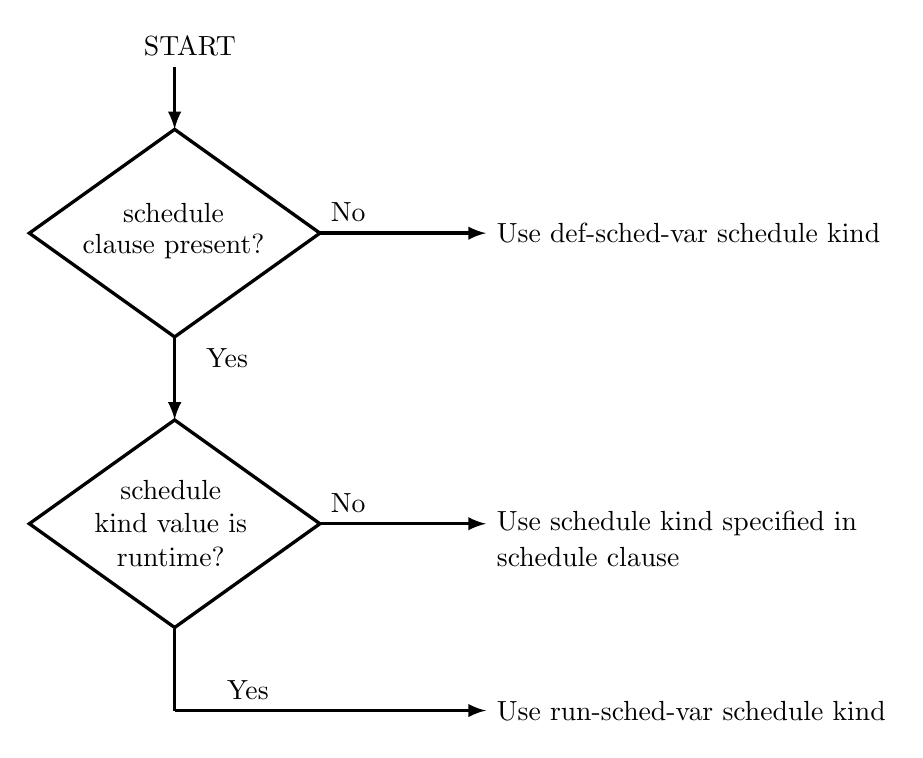
\begin{tikzpicture}
\pgftransformxscale{1.000000}
\pgftransformyscale{-1.000000}
\definecolor{dialinecolor}{rgb}{0.000000, 0.000000, 0.000000}
\pgfsetstrokecolor{dialinecolor}
\definecolor{dialinecolor}{rgb}{1.000000, 1.000000, 1.000000}
\pgfsetfillcolor{dialinecolor}
\definecolor{dialinecolor}{rgb}{1.000000, 1.000000, 1.000000}
\pgfsetfillcolor{dialinecolor}
\fill (18.500000\du,7.000000\du)--(22.000000\du,9.500000\du)--(18.500000\du,12.000000\du)--(15.000000\du,9.500000\du)--cycle;
\pgfsetlinewidth{0.080000\du}
\pgfsetdash{}{0pt}
\pgfsetdash{}{0pt}
\pgfsetmiterjoin
\definecolor{dialinecolor}{rgb}{0.000000, 0.000000, 0.000000}
\pgfsetstrokecolor{dialinecolor}
\draw (18.500000\du,7.000000\du)--(22.000000\du,9.500000\du)--(18.500000\du,12.000000\du)--(15.000000\du,9.500000\du)--cycle;
% setfont left to latex
\definecolor{dialinecolor}{rgb}{0.000000, 0.000000, 0.000000}
\pgfsetstrokecolor{dialinecolor}
\node at (18.500000\du,9.695000\du){};
\pgfsetlinewidth{0.080000\du}
\pgfsetdash{}{0pt}
\pgfsetdash{}{0pt}
\pgfsetbuttcap
{
\definecolor{dialinecolor}{rgb}{0.000000, 0.000000, 0.000000}
\pgfsetfillcolor{dialinecolor}
% was here!!!
\pgfsetarrowsend{latex}
\definecolor{dialinecolor}{rgb}{0.000000, 0.000000, 0.000000}
\pgfsetstrokecolor{dialinecolor}
\draw (18.500000\du,12.000000\du)--(18.500000\du,14.000000\du);
}
\pgfsetlinewidth{0.080000\du}
\pgfsetdash{}{0pt}
\pgfsetdash{}{0pt}
\pgfsetbuttcap
{
\definecolor{dialinecolor}{rgb}{0.000000, 0.000000, 0.000000}
\pgfsetfillcolor{dialinecolor}
% was here!!!
\pgfsetarrowsend{latex}
\definecolor{dialinecolor}{rgb}{0.000000, 0.000000, 0.000000}
\pgfsetstrokecolor{dialinecolor}
\draw (22.000000\du,16.500000\du)--(26.000000\du,16.500000\du);
}
% setfont left to latex
\definecolor{dialinecolor}{rgb}{0.000000, 0.000000, 0.000000}
\pgfsetstrokecolor{dialinecolor}
\node[anchor=west] at (20.000000\du,10.000000\du){};
\pgfsetlinewidth{0.080000\du}
\pgfsetdash{}{0pt}
\pgfsetdash{}{0pt}
\pgfsetbuttcap
{
\definecolor{dialinecolor}{rgb}{0.000000, 0.000000, 0.000000}
\pgfsetfillcolor{dialinecolor}
% was here!!!
\pgfsetarrowsend{latex}
\definecolor{dialinecolor}{rgb}{0.000000, 0.000000, 0.000000}
\pgfsetstrokecolor{dialinecolor}
\draw (18.500000\du,5.500000\du)--(18.500000\du,7.000000\du);
}
% setfont left to latex
\definecolor{dialinecolor}{rgb}{0.000000, 0.000000, 0.000000}
\pgfsetstrokecolor{dialinecolor}
\node[anchor=west] at (31.000000\du,12.000000\du){};
\definecolor{dialinecolor}{rgb}{1.000000, 1.000000, 1.000000}
\pgfsetfillcolor{dialinecolor}
\fill (18.500000\du,14.000000\du)--(22.000000\du,16.500000\du)--(18.500000\du,19.000000\du)--(15.000000\du,16.500000\du)--cycle;
\pgfsetlinewidth{0.080000\du}
\pgfsetdash{}{0pt}
\pgfsetdash{}{0pt}
\pgfsetmiterjoin
\definecolor{dialinecolor}{rgb}{0.000000, 0.000000, 0.000000}
\pgfsetstrokecolor{dialinecolor}
\draw (18.500000\du,14.000000\du)--(22.000000\du,16.500000\du)--(18.500000\du,19.000000\du)--(15.000000\du,16.500000\du)--cycle;
% setfont left to latex
\definecolor{dialinecolor}{rgb}{0.000000, 0.000000, 0.000000}
\pgfsetstrokecolor{dialinecolor}
\node at (18.500000\du,16.695000\du){};
\pgfsetlinewidth{0.080000\du}
\pgfsetdash{}{0pt}
\pgfsetdash{}{0pt}
\pgfsetbuttcap
{
\definecolor{dialinecolor}{rgb}{0.000000, 0.000000, 0.000000}
\pgfsetfillcolor{dialinecolor}
% was here!!!
\pgfsetarrowsend{latex}
\definecolor{dialinecolor}{rgb}{0.000000, 0.000000, 0.000000}
\pgfsetstrokecolor{dialinecolor}
\draw (22.000000\du,9.500000\du)--(26.000000\du,9.500000\du);
}
\pgfsetlinewidth{0.080000\du}
\pgfsetdash{}{0pt}
\pgfsetdash{}{0pt}
\pgfsetbuttcap
{
\definecolor{dialinecolor}{rgb}{0.000000, 0.000000, 0.000000}
\pgfsetfillcolor{dialinecolor}
% was here!!!
\definecolor{dialinecolor}{rgb}{0.000000, 0.000000, 0.000000}
\pgfsetstrokecolor{dialinecolor}
\draw (18.500000\du,19.040000\du)--(18.500000\du,21.000000\du);
}
\pgfsetlinewidth{0.080000\du}
\pgfsetdash{}{0pt}
\pgfsetdash{}{0pt}
\pgfsetbuttcap
{
\definecolor{dialinecolor}{rgb}{0.000000, 0.000000, 0.000000}
\pgfsetfillcolor{dialinecolor}
% was here!!!
\pgfsetarrowsend{latex}
\definecolor{dialinecolor}{rgb}{0.000000, 0.000000, 0.000000}
\pgfsetstrokecolor{dialinecolor}
\draw (18.500000\du,21.000000\du)--(26.000000\du,21.000000\du);
}
% setfont left to latex
\definecolor{dialinecolor}{rgb}{0.000000, 0.000000, 0.000000}
\pgfsetstrokecolor{dialinecolor}
\node[anchor=west] at (17.500000\du,5.000000\du){START};
% setfont left to latex
\definecolor{dialinecolor}{rgb}{0.000000, 0.000000, 0.000000}
\pgfsetstrokecolor{dialinecolor}
\node at (18.471967\du,9.021967\du){\code{schedule} 
};
% setfont left to latex
\definecolor{dialinecolor}{rgb}{0.000000, 0.000000, 0.000000}
\pgfsetstrokecolor{dialinecolor}
\node at (18.471967\du,9.821967\du){clause present?};
% setfont left to latex
\definecolor{dialinecolor}{rgb}{0.000000, 0.000000, 0.000000}
\pgfsetstrokecolor{dialinecolor}
\node at (18.408579\du,15.687353\du){schedule};
% setfont left to latex
\definecolor{dialinecolor}{rgb}{0.000000, 0.000000, 0.000000}
\pgfsetstrokecolor{dialinecolor}
\node at (18.408579\du,16.487353\du){kind value is};
% setfont left to latex
\definecolor{dialinecolor}{rgb}{0.000000, 0.000000, 0.000000}
\pgfsetstrokecolor{dialinecolor}
\node at (18.408579\du,17.287353\du){\code{runtime}?};
% setfont left to latex
\definecolor{dialinecolor}{rgb}{0.000000, 0.000000, 0.000000}
\pgfsetstrokecolor{dialinecolor}
\node[anchor=west] at (26.000000\du,9.500000\du){Use \plc{def-sched-var} schedule kind};
% setfont left to latex
\definecolor{dialinecolor}{rgb}{0.000000, 0.000000, 0.000000}
\pgfsetstrokecolor{dialinecolor}
\node[anchor=west] at (26.000000\du,16.500000\du){Use schedule kind specified in 
};
% setfont left to latex
\definecolor{dialinecolor}{rgb}{0.000000, 0.000000, 0.000000}
\pgfsetstrokecolor{dialinecolor}
\node[anchor=west] at (26.000000\du,17.300000\du){\code{schedule} clause};
% setfont left to latex
\definecolor{dialinecolor}{rgb}{0.000000, 0.000000, 0.000000}
\pgfsetstrokecolor{dialinecolor}
\node[anchor=west] at (26.000000\du,21.000000\du){Use \plc{run-sched-var} schedule kind};
% setfont left to latex
\definecolor{dialinecolor}{rgb}{0.000000, 0.000000, 0.000000}
\pgfsetstrokecolor{dialinecolor}
\node[anchor=west] at (22.000000\du,9.000000\du){No};
% setfont left to latex
\definecolor{dialinecolor}{rgb}{0.000000, 0.000000, 0.000000}
\pgfsetstrokecolor{dialinecolor}
\node[anchor=west] at (19.000000\du,12.500000\du){Yes};
% setfont left to latex
\definecolor{dialinecolor}{rgb}{0.000000, 0.000000, 0.000000}
\pgfsetstrokecolor{dialinecolor}
\node[anchor=west] at (22.000000\du,16.000000\du){No};
% setfont left to latex
\definecolor{dialinecolor}{rgb}{0.000000, 0.000000, 0.000000}
\pgfsetstrokecolor{dialinecolor}
\node[anchor=west] at (19.500000\du,20.500000\du){Yes};
\end{tikzpicture}

\end{quote}
\caption{Determining the \code{schedule} for a Worksharing Loop\label{fig:schedule loop}}
\end{figure}

\crossreferences
\begin{itemize}
\item ICVs, see
\specref{sec:Internal Control Variables}
\end{itemize}











\subsection{\hcode{sections} Construct}
\label{subsec:sections Construct}
\index{sections@{\code{sections}}}
\index{constructs!sections@{\code{sections}}}
\summary
The \code{sections} construct is a non-iterative worksharing construct that contains a set of
structured blocks that are to be distributed among and executed by the threads in a team.
Each structured block is executed once by one of the threads in the team in the context
of its implicit task.

\syntax
\begin{ccppspecific}
The syntax of the \code{sections} construct is as follows:

\begin{ompcPragma}
#pragma omp sections \plc{[clause[ [},\plc{] clause] ... ] new-line}
   {
   \plc{[}#pragma omp section \plc{new-line}\plc{]}
      \plc{structured-block}
   \plc{[}#pragma omp section \plc{new-line}
      \plc{structured-block]}
   \plc{...}
   }
\end{ompcPragma}

where \plc{clause} is one of the following:

\begin{indentedcodelist}
private(\plc{list})
firstprivate(\plc{list})
lastprivate(\plc{[ lastprivate-modifier}:\plc{] list})
reduction(\plc{reduction-identifier }:\plc{ list})
nowait
allocate(\plc{[allocator: ]}\plc{list})
\end{indentedcodelist}
\end{ccppspecific}

\needspace{16\baselineskip}
\begin{fortranspecific}
The syntax of the \code{sections} construct is as follows:

\begin{ompfPragma}
!$omp sections \plc{[clause[ [},\plc{] clause] ... ]}
   \plc{[}!$omp section\plc{]}
      \plc{structured-block}
   \plc{[}!$omp section
      \plc{structured-block]}
   \plc{...}
!$omp end sections \plc{[}nowait\plc{]}
\end{ompfPragma}

\begin{samepage}
where \plc{clause} is one of the following:

\begin{indentedcodelist}
private(\plc{list})
firstprivate(\plc{list})
lastprivate(\plc{[ lastprivate-modifier}:\plc{] list})
reduction(\plc{reduction-identifier }:\plc{ list})
allocate(\plc{[allocator: ]}\plc{list})
\end{indentedcodelist}
\end{samepage}
\end{fortranspecific}

\binding
The binding thread set for a \code{sections} region is the current team. A \code{sections}
region binds to the innermost enclosing \code{parallel} region. Only the threads of the team
executing the binding \code{parallel} region participate in the execution of the structured
blocks and the implied barrier of the \code{sections} region if the barrier is not eliminated
by a \code{nowait} clause.

\descr
Each structured block in the \code{sections} construct is preceded by a \code{section} directive
except possibly the first block, for which a preceding \code{section} directive is optional.

The method of scheduling the structured blocks among the threads in the team is
implementation defined.

There is an implicit barrier at the end of a \code{sections} construct unless a \code{nowait}
clause is specified.

%\tools
\omptWorksharing{sections}{ompt\_work\_sections}

\restrictions
Restrictions to the \code{sections} construct are as follows:

\begin{itemize}
\item Orphaned \code{section} directives are prohibited. That is, the \code{section} directives must
appear within the \code{sections} construct and must not be encountered elsewhere in the
\code{sections} region.

\item The code enclosed in a \code{sections} construct must be a structured block.

\item Only a single \code{nowait} clause can appear on a \code{sections} directive.

\begin{cppspecific}
\item A throw executed inside a \code{sections} region must cause execution to resume within
the same section of the \code{sections} region, and the same thread that threw the
exception must catch it.
\end{cppspecific}
\end{itemize}

\crossreferences
\begin{itemize}
\item \code{private}, \code{firstprivate}, \code{lastprivate}, and \code{reduction} clauses, see
\specref{subsec:Data-Sharing Attribute Clauses}.

\item \code{ompt_scope_begin} and \code{ompt_scope_end}, see
  \specref{sec:ompt_scope_endpoint_t}.

\item \code{ompt_work_sections}, see \specref{sec:ompt_work_type_t}.

\item \code{ompt_callback_work_t}, see
\specref{sec:ompt_callback_work_t}.
\end{itemize}










\subsection{\hcode{single} Construct}
\index{single@{\code{single}}}
\index{constructs!single@{\code{single}}}
\label{subsec:single Construct}
\summary
The \code{single} construct specifies that the associated structured block is executed by only
one of the threads in the team (not necessarily the master thread), in the context of its
implicit task. The other threads in the team, which do not execute the block, wait at an
implicit barrier at the end of the \code{single} construct unless a \code{nowait} clause is specified.

\syntax
\begin{ccppspecific}
The syntax of the single construct is as follows:

\begin{ompcPragma}
#pragma omp single \plc{[clause[ [},\plc{] clause] ... ] new-line}
   \plc{structured-block}
\end{ompcPragma}

\begin{samepage}
where \plc{clause} is one of the following:

\begin{indentedcodelist}
private(\plc{list})
firstprivate(\plc{list})
copyprivate(\plc{list})
nowait
allocate(\plc{[allocator: ]}\plc{list})
\end{indentedcodelist}
\end{samepage}
\end{ccppspecific}

\begin{fortranspecific}
The syntax of the \code{single} construct is as follows:

\begin{ompfPragma}
!$omp single \plc{[clause[ [},\plc{] clause] ... ]}
   \plc{structured-block}
!$omp end single \plc{[end_clause[ [},\plc{] end_clause] ... ]}
\end{ompfPragma}

where \plc{clause} is one of the following:

\begin{indentedcodelist}
private(\plc{list})
firstprivate(\plc{list})
allocate(\plc{[allocator: ]}\plc{list})
\end{indentedcodelist}

and \plc{end_clause} is one of the following:

\begin{indentedcodelist}
copyprivate(\plc{list})
nowait
\end{indentedcodelist}
\end{fortranspecific}

\binding
The binding thread set for a \code{single} region is the current team. A \code{single} region
binds to the innermost enclosing \code{parallel} region. Only the threads of the team
executing the binding \code{parallel} region participate in the execution of the structured
block and the implied barrier of the \code{single} region if the barrier is not eliminated by a
\code{nowait} clause.

\descr
Only one of the encountering threads will execute the structured block associated with the \code{single}
construct. The method of choosing a thread to execute the structured block each time the team encounters the construct
is implementation defined. There is an implicit barrier at the end of the \code{single} construct unless a
\code{nowait} clause is specified.

\events

The \plc{single-begin} event occurs after an \code{implicit task} encounters a
\code{single} construct but before the task starts the execution of the structured
block of the \code{single} region.

The \plc{single-end} event occurs after a \code{single} region finishes execution of the structured block
but before resuming execution of the encountering implicit task.


\tools

A thread dispatches a registered \code{ompt_callback_work}
callback for each occurrence of \plc{single-begin} and
\plc{single-end} events in that thread. The callback has type signature
\code{ompt_callback_work_t}. The callback receives
\code{ompt_scope_begin} or \code{ompt_scope_end}
as its \plc{endpoint} argument, as appropriate, and
\code{ompt_work_single_executor} or \code{ompt_work_single_other}
as its \plc{wstype} argument.

\restrictions
Restrictions to the \code{single} construct are as follows:

\begin{itemize}
\item The \code{copyprivate} clause must not be used with the \code{nowait} clause.

\item At most one \code{nowait} clause can appear on a \code{single} construct.

\begin{cppspecific}
\item A throw executed inside a \code{single} region must cause execution to resume within the
same \code{single} region, and the same thread that threw the exception must catch it.
\end{cppspecific}
\end{itemize}


\crossreferences
\begin{itemize}
\item \code{private} and \code{firstprivate} clauses, see
\specref{subsec:Data-Sharing Attribute Clauses}.

\item \code{copyprivate} clause, see
\specref{subsubsec:copyprivate clause}.

\item \code{ompt_scope_begin} and \code{ompt_scope_end}, see
  \specref{sec:ompt_scope_endpoint_t}.

\item \code{ompt_work_single_executor} and \code{ompt_work_single_other}, see
\specref{sec:ompt_work_type_t}.

\item \code{ompt_callback_work_t},
\specref{sec:ompt_callback_work_t}.

\end{itemize}












%\newpage %% HACK

% Here we need to force the blue marker lower, and force the subsection header higher
% in order to reduce the space between the marker and the header, per Richard:
%\begin{samepage}
\vspace{3\baselineskip}
\begin{fortranspecific}
\vspace{-1\baselineskip}
\subsection{\hcode{workshare} Construct}
\index{workshare@{\code{workshare}}}
\index{constructs!workshare@{\code{workshare}}}
\label{subsec:workshare Construct}
\summary
The \code{workshare} construct divides the execution of the enclosed structured block into
separate units of work, and causes the threads of the team to share the work such that
each unit is executed only once by one thread, in the context of its implicit task.
%\end{samepage}

%\begin{samepage}
\syntax
The syntax of the \code{workshare} construct is as follows:

\begin{ompfPragma}
!$omp workshare
    \plc{structured-block}
!$omp end workshare \plc{[}nowait\plc{]}
\end{ompfPragma}
%\end{samepage}

The enclosed structured block must consist of only the following:

\begin{itemize}
\item array assignments

\item scalar assignments

\item \code{FORALL} statements

\item \code{FORALL} constructs

\item \code{WHERE} statements

\item \code{WHERE} constructs

\item \code{atomic} constructs

\item \code{critical} constructs

\item \code{parallel} constructs
\end{itemize}

Statements contained in any enclosed \code{critical} construct are also subject to these
restrictions. Statements in any enclosed \code{parallel} construct are not restricted.

\binding
The binding thread set for a \code{workshare} region is the current team. A \code{workshare}
region binds to the innermost enclosing \code{parallel} region. Only the threads of the team
executing the binding \code{parallel} region participate in the execution of the units of
work and the implied barrier of the \code{workshare} region if the barrier is not eliminated
by a \code{nowait} clause.

\descr
There is an implicit barrier at the end of a \code{workshare} construct unless a \code{nowait}
clause is specified.

An implementation of the \code{workshare} construct must insert any synchronization that is
required to maintain standard Fortran semantics. For example, the effects of one
statement within the structured block must appear to occur before the execution of
succeeding statements, and the evaluation of the right hand side of an assignment must
appear to complete prior to the effects of assigning to the left hand side.

The statements in the \code{workshare} construct are divided into units of work as follows:

\begin{itemize}
\item For array expressions within each statement, including transformational array
intrinsic functions that compute scalar values from arrays:

\begin{itemize} % nested level
\item Evaluation of each element of the array expression, including any references to
\code{ELEMENTAL} functions, is a unit of work.

\item Evaluation of transformational array intrinsic functions may be freely subdivided
into any number of units of work.
\end{itemize}

\item For an array assignment statement, the assignment of each element is a unit of work.

\item For a scalar assignment statement, the assignment operation is a unit of work.

\item For a \code{WHERE} statement or construct, the evaluation of the mask expression and the
masked assignments are each a unit of work.

\item For a \code{FORALL} statement or construct, the evaluation of the mask expression,
expressions occurring in the specification of the iteration space, and the masked
assignments are each a unit of work

\item For an \code{atomic} construct, the atomic operation on the storage location designated as
\plc{x} is a unit of work.

\item For a \code{critical} construct, the construct is a single unit of work.

\item For a \code{parallel} construct, the construct is a unit of work with respect to the
\code{workshare} construct. The statements contained in the \code{parallel} construct are
executed by a new thread team.

\item If none of the rules above apply to a portion of a statement in the structured block,
then that portion is a unit of work.
\end{itemize}

The transformational array intrinsic functions are \code{MATMUL}, \code{DOT_PRODUCT}, \code{SUM},
\code{PRODUCT}, \code{MAXVAL}, \code{MINVAL}, \code{COUNT},
\code{ANY}, \code{ALL}, \code{SPREAD}, \code{PACK}, \code{UNPACK},
\code{RESHAPE}, \code{TRANSPOSE}, \code{EOSHIFT}, \code{CSHIFT}, \code{MINLOC}, and \code{MAXLOC}.

It is unspecified how the units of work are assigned to the threads executing a
\code{workshare} region.

If an array expression in the block references the value, association status, or allocation
status of private variables, the value of the expression is undefined, unless the same
value would be computed by every thread.

If an array assignment, a scalar assignment, a masked array assignment, or a \code{FORALL}
assignment assigns to a private variable in the block, the result is unspecified.

The \code{workshare} directive causes the sharing of work to occur only in the \code{workshare}
construct, and not in the remainder of the \code{workshare} region.

%\tools
\omptWorksharing{workshare}{ompt\_work\_workshare}

\begin{samepage}
\restrictions
The following restrictions apply to the \code{workshare} construct:

\begin{itemize}
\item All array assignments, scalar assignments, and masked array assignments must be
intrinsic assignments.

\item The construct must not contain any user defined function calls unless the function is
\code{ELEMENTAL}.
\end{itemize}
\end{samepage}

\crossreferences
\begin{itemize}
\item \code{ompt_scope_begin} and \code{ompt_scope_end}, see
  \specref{sec:ompt_scope_endpoint_t}.
\item \code{ompt_work_workshare}, see \specref{sec:ompt_work_type_t}.
\item \code{ompt_callback_work_t}, see
\specref{sec:ompt_callback_work_t}.
\end{itemize}

%\filbreak
\end{fortranspecific}

% This is an included file. See the master file for more information.
%
% When editing this file:
%
%    1. To change formatting, appearance, or style, please edit openmp.sty.
%
%    2. Custom commands and macros are defined in openmp.sty.
%
%    3. Be kind to other editors -- keep a consistent style by copying-and-pasting to
%       create new content.
%
%    4. We use semantic markup, e.g. (see openmp.sty for a full list):
%         \code{}     % for bold monospace keywords, code, operators, etc.
%         \plc{}      % for italic placeholder names, grammar, etc.
%
%    5. There are environments that provide special formatting, e.g. language bars.
%       Please use them whereever appropriate.  Examples are:
%
%         \begin{fortranspecific}
%         This is text that appears enclosed in blue language bars for Fortran.
%         \end{fortranspecific}
%
%         \begin{note}
%         This is a note.  The "Note -- " header appears automatically.
%         \end{note}
%
%    6. Other recommendations:
%         Use the convenience macros defined in openmp.sty for the minor headers
%         such as Comments, Syntax, etc.
%
%         To keep items together on the same page, prefer the use of 
%         \begin{samepage}.... Avoid \parbox for text blocks as it interrupts line numbering.
%         When possible, avoid \filbreak, \pagebreak, \newpage, \clearpage unless that's
%         what you mean. Use \needspace{} cautiously for troublesome paragraphs.
%
%         Avoid absolute lengths and measures in this file; use relative units when possible.
%         Vertical space can be relative to \baselineskip or ex units. Horizontal space
%         can be relative to \linewidth or em units.
%
%         Prefer \emph{} to italicize terminology, e.g.:
%             This is a \emph{definition}, not a placeholder.
%             This is a \plc{var-name}.
%


\section{SIMD Constructs}
\label{sec:SIMD Constructs}
\index{SIMD Constructs}
\subsection{\code{simd} Construct}
\index{simd@{\code{simd}}}
\index{constructs!simd@{\code{simd}}}
\label{subsec:simd Construct}
\summary
The \code{simd} construct can be applied to a loop to indicate that the loop can be transformed 
into a SIMD loop (that is, multiple iterations of the loop can be executed concurrently 
using SIMD instructions).

\syntax
The syntax of the \code{simd} construct is as follows:

\begin{ccppspecific}
\begin{boxedcode}
\#pragma omp simd \plc{[clause[ [},\plc{] clause] ... ] new-line}
   \plc{for-loops}
\end{boxedcode}

where \plc{clause} is one of the following:

\begin{indentedcodelist}
safelen(\plc{length})
simdlen(\plc{length})
linear(\plc{list[ }:\plc{ linear-step]})
aligned(\plc{list[ }:\plc{ alignment]})
nontemporal(\plc{list})
private(\plc{list})
lastprivate(\plc{[ lastprivate-modifier}:\plc{] list})
reduction(\plc{reduction-identifier }:\plc{ list})
collapse(\plc{n})
\end{indentedcodelist}

The \code{simd} directive places restrictions on the structure of the associated \plc{for-loops}. 
Specifically, all associated \plc{for-loops} must have \plc{canonical loop form} 
(\specref{sec:Canonical Loop Form}).
\end{ccppspecific}

\begin{fortranspecific}
\begin{boxedcode}
!\$omp simd \plc{[clause[ [},\plc{] clause ... ]}
   \plc{do-loops}
\plc{[}!\$omp end simd\plc{]}
\end{boxedcode}

where \plc{clause} is one of the following:

\begin{indentedcodelist}
safelen(\plc{length})
simdlen(\plc{length})
linear(\plc{list[ }:\plc{ linear-step]})
aligned(\plc{list[ }:\plc{ alignment]})
nontemporal(\plc{list})
private(\plc{list})
lastprivate(\plc{[ lastprivate-modifier}:\plc{] list})
reduction(\plc{reduction-identifier }:\plc{ list})
collapse(\plc{n})
\end{indentedcodelist}

If an \code{end}~\code{simd} directive is not specified, an \code{end}~\code{simd} directive is assumed at the end 
of the \plc{do-loops}.

Any associated \plc{do-loop} must be a \plc{do-construct} or an 
\plc{inner-shared-do-construct} as defined by the Fortran standard. If an 
\code{end}~\code{simd} directive follows a \plc{do-construct} in which 
several loop statements share a \code{DO} termination statement, then the 
directive can only be specified for the outermost of these 
\code{DO} statements. 
\end{fortranspecific}

\binding
A \code{simd} region binds to the current task region. The binding thread set of the \code{simd} 
region is the current team.

\descr
The \code{simd} construct enables the execution of multiple iterations of the associated loops 
concurrently by means of SIMD instructions.

The \code{collapse} clause may be used to specify how many loops are associated with the 
construct. The parameter of the \code{collapse} clause must be a constant positive integer 
expression. If no \code{collapse} clause is present, the only loop that is associated with the 
loop construct is the one that immediately follows the directive.

If more than one loop is associated with the \code{simd} construct, then the iterations of all 
associated loops are collapsed into one larger iteration space that is then executed with 
SIMD instructions. The sequential execution of the iterations in all associated loops 
determines the order of the iterations in the collapsed iteration space.

The iteration count for each associated loop is computed before entry to the outermost 
loop. If execution of any associated loop changes any of the values used to compute any 
of the iteration counts, then the behavior is unspecified.

The integer type (or kind, for Fortran) used to compute the iteration count for the 
collapsed loop is implementation defined.

A SIMD loop has logical iterations numbered 0,1,...,N-1 where N is the number of loop 
iterations, and the logical numbering denotes the sequence in which the iterations would 
be executed if the associated loop(s) were executed with no SIMD instructions. If the 
\code{safelen} clause is used then no two iterations executed concurrently with SIMD 
instructions can have a greater distance in the logical iteration space than its value. The 
parameter of the \code{safelen} clause must be a constant positive integer expression. 
If used, the \code{simdlen} clause specifies the preferred number of iterations to be executed concurrently. 
The parameter of the \code{simdlen} clause must be a constant positive integer.
The number of iterations that are executed concurrently at any given time is implementation 
defined. Each concurrent iteration will be executed by a different SIMD lane. Each set 
of concurrent iterations is a SIMD chunk. Lexical forward dependencies in the iterations of the original loop must be preserved within each SIMD chunk.

\begin{ccppspecific}
The \code{aligned} clause declares that the object to which each list item points is aligned to 
the number of bytes expressed in the optional parameter of the \code{aligned} clause.
\end{ccppspecific}

\begin{fortranspecific}

The \code{aligned} clause declares that the location of each list item
is aligned to the number of bytes expressed in the optional parameter
of the \code{aligned} clause.

\end{fortranspecific}

The optional parameter of the \code{aligned} clause, \plc{alignment}, must be a constant positive 
integer expression. If no optional parameter is specified, implementation-defined default 
alignments for SIMD instructions on the target platforms are assumed.

The \code{nontemporal} clause specifies that for the objects to which each list item refers is not re-accessed (written or read) within the loop associated with the \code{simd} construct after the first access.
The effect of the \code{nontemporal} clause is implementation-defined and can be ignored by the implementation.

\restrictions
\begin{itemize}
\item All loops associated with the construct must be perfectly nested; that is, there must be 
no intervening code nor any OpenMP directive between any two loops.

\item The associated loops must be structured blocks.

\item A program that branches into or out of a \code{simd} region is non-conforming. 

\item Only one \code{collapse} clause can appear on a \code{simd} directive.

\item A \plc{list-item} cannot appear in more than one \code{aligned} clause.

\item Only one \code{safelen} clause can appear on a \code{simd} directive.

\item Only one \code{simdlen} clause can appear on a \code{simd} directive.

\item If both \code{simdlen} and \code{safelen} clauses are specified, the value of the \code{simdlen} parameter must be less than or equal to the value of the \code{safelen} parameter.

\item A \plc{modifier} may not be specified on a \code{linear} clause.

\item An \code{ordered} construct with the \code{simd} clause is the only OpenMP
construct that can be encountered during execution of a \code{simd}
region.

\begin{ccppspecific}
\item The \code{simd} region cannot contain calls to the \code{longjmp} or \code{setjmp} functions. 
\end{ccppspecific}
\bigskip

\begin{cspecific}
\item The type of list items appearing in the \code{aligned} clause must be array or pointer.
\end{cspecific}

\begin{cppspecific}
\item The type of list items appearing in the \code{aligned} clause must be array, pointer, 
reference to array, or reference to pointer. 

\item No exception can be raised in the \code{simd} region. 
\end{cppspecific}

\begin{fortranspecific}
\item The \plc{do-loop} iteration variable must be of type \code{integer}.

\item The \plc{do-loop} cannot be a \code{DO WHILE} or a \code{DO} loop without loop control. 

\item If a list item on the \code{aligned} clause has the
  \code{ALLOCATABLE} attribute, the allocation status must be
  allocated.

\item If a list item on the \code{aligned} clause has the
  \code{POINTER} attribute, the association status must be associated.

\item If the type of a list item on the \code{aligned} clause is
  either \code{C\_PTR} or Cray pointer, the list item must be defined.

\end{fortranspecific}
\end{itemize}

\crossreferences
\begin{itemize}
\item \code{private}, \code{lastprivate}, \code{linear} and \code{reduction} clauses, see 
\specref{subsec:Data-Sharing Attribute Clauses}.
\end{itemize}








\subsection{\code{declare}~\code{simd} Construct}
\index{declare simd@{\code{declare}~\code{simd}}}
\index{constructs!declare simd@{\code{declare}~\code{simd}}}
\label{subsec:declare simd Construct}
\summary
The \code{declare}~\code{simd} construct can be applied to a function (C, C++ and Fortran) or a 
subroutine (Fortran) to enable the creation of one or more versions that can process 
multiple arguments using SIMD instructions from a single invocation in a SIMD 
loop. The \code{declare}~\code{simd} directive is a declarative directive. There may be multiple 
\code{declare}~\code{simd} directives for a function (C, C++, Fortran) or subroutine (Fortran).

\syntax
The syntax of the \code{declare}~\code{simd} construct is as follows:

\begin{ccppspecific}
\begin{boxedcode}
\#pragma omp declare simd \plc{[clause[ [},\plc{] clause] ... ] new-line}
\plc{[}\#pragma omp declare simd \plc{[clause[ [},\plc{] clause] ... ] new-line]}
\plc{[ ... ]}
   \plc{function definition or declaration}
\end{boxedcode}

where \plc{clause} is one of the following:

\begin{indentedcodelist}
simdlen(\plc{length})
linear(\plc{linear-list[ }:\plc{ linear-step]})
aligned(\plc{argument-list[ }:\plc{ alignment]})
uniform(\plc{argument-list})
inbranch
notinbranch
\end{indentedcodelist}
\end{ccppspecific}


\begin{fortranspecific}
\begin{boxedcode}
!\$omp declare simd \plc{[}(\plc{proc-name})\plc{] [clause[ [},\plc{] clause] ... ]}
\end{boxedcode}

where \plc{clause} is one of the following:
\begin{indentedcodelist}
simdlen(\plc{length})
linear(\plc{linear-list[ }:\plc{ linear-step]})
aligned(\plc{argument-list[ }:\plc{ alignment]})
uniform(\plc{argument-list})
inbranch
notinbranch
\end{indentedcodelist}
\end{fortranspecific}


\descr
\begin{ccppspecific}
The use of a \code{declare}~\code{simd} construct on a function enables the creation of SIMD 
versions of the associated function that can be used to process multiple arguments from 
a single invocation in a SIMD loop concurrently.

The expressions appearing in the clauses of this directive are evaluated in the scope of 
the arguments of the function declaration or definition.
\end{ccppspecific}

\begin{samepage}
\begin{fortranspecific}
The use of a \code{declare}~\code{simd} construct enables the creation of SIMD versions of the 
specified subroutine or function that can be used to process multiple arguments from a 
single invocation in a SIMD loop concurrently. 
\end{fortranspecific}
\end{samepage}

If a \code{declare}~\code{simd} directive contains multiple SIMD declarations,
each declaration enables the creation of SIMD versions.

If a SIMD version is created, the number of concurrent arguments for the function is 
determined by the \code{simdlen} clause. If the \code{simdlen} clause is used its value 
corresponds to the number of concurrent arguments of the function. The parameter of 
the \code{simdlen} clause must be a constant positive integer expression. Otherwise, the 
number of concurrent arguments for the function is implementation defined.

\begin{cppspecific}
The special \plc{this} pointer can be used as if was one of the arguments to the function in any of the \code{linear}, \code{aligned}, or \code{uniform} clauses.
\end{cppspecific}

The \code{uniform} clause declares one or more arguments to have an invariant value for all 
concurrent invocations of the function in the execution of a single SIMD loop.

\begin{samepage}
\begin{ccppspecific}
The \code{aligned} clause declares that the object to which each list item points is aligned to 
the number of bytes expressed in the optional parameter of the \code{aligned} clause.
\end{ccppspecific}
\end{samepage}

\needspace{15\baselineskip}\begin{samepage}
\begin{fortranspecific}
The \code{aligned} clause declares that the target of each list item is aligned to the number 
of bytes expressed in the optional parameter of the \code{aligned} clause.
\end{fortranspecific}
\end{samepage}

The optional parameter of the \code{aligned} clause, \plc{alignment}, must be a constant positive 
integer expression. If no optional parameter is specified, implementation-defined default 
alignments for SIMD instructions on the target platforms are assumed.

The \code{inbranch} clause specifies that the SIMD version of the function will always be called from inside a 
conditional statement of a SIMD loop. The \code{notinbranch} clause specifies that the 
SIMD version of the function will never be called from inside a conditional statement of a SIMD loop. If 
neither clause is specified, then the SIMD version of the function may or may not be called from inside a 
conditional statement of a SIMD loop.

\restrictions
\begin{itemize}
\item Each argument can appear in at most one \code{uniform} or \code{linear} clause.

\item At most one \code{simdlen} clause can appear in a \code{declare}~\code{simd} directive.

\item Either \code{inbranch} or \code{notinbranch} may be specified, but not both.

\item When a \plc{linear-step} expression is specified in a \code{linear} clause it must be
either a constant integer expression or an integer-typed parameter that is specified in
a \code{uniform} clause on the directive.

\item The function or subroutine body must be a structured block.

\item The execution of the function or subroutine, when called from a SIMD loop, cannot result in the execution of an OpenMP construct except for an \code{ordered} construct with the \code{simd} clause. 

\item The execution of the function or subroutine cannot have any side effects that would 
alter its execution for concurrent iterations of a SIMD chunk.

\item A program that branches into or out of the function is non-conforming.

\begin{ccppspecific}
\item If the function has any declarations, then the \code{declare}~\code{simd} construct for any 
declaration that has one must be equivalent to the one specified for the definition. 
Otherwise, the result is unspecified.

\item The function cannot contain calls to the \code{longjmp} or \code{setjmp} functions. 
\end{ccppspecific}

\begin{cspecific}
\item The type of list items appearing in the \code{aligned} clause must be array or pointer. 
\end{cspecific}

\begin{cppspecific}
\item The function cannot contain any calls to \code{throw}. 

\item The type of list items appearing in the \code{aligned} clause must be array, pointer, 
reference to array, or reference to pointer.
\end{cppspecific}

\begin{fortranspecific}
\item \plc{proc-name} must not be a generic name, procedure pointer or entry name.

\item If \plc{proc-name} is omitted, the \code{declare}~\code{simd}
  directive must appear in the specification part of a subroutine
  subprogram or a function subprogram for which creation of the SIMD
  versions is enabled.

\item Any \code{declare}~\code{simd} directive must appear in the specification part of a subroutine 
subprogram, function subprogram or interface body to which it applies.

\item If a \code{declare}~\code{simd} directive is specified in an interface block for a procedure, it 
must match a \code{declare}~\code{simd} directive in the definition of the procedure.

\item If a procedure is declared via a procedure declaration statement, the procedure 
\plc{proc-name} should appear in the same specification. 

\item If a \code{declare}~\code{simd} directive is specified for a procedure name with explicit 
interface and a \code{declare}~\code{simd} directive is also specified for the definition of the 
procedure then the two \code{declare}~\code{simd} directives must match. Otherwise the result 
is unspecified.

\item Procedure pointers may not be used to access versions created by the \code{declare}~\code{simd} directive.

\item The type of list items appearing in the \code{aligned} clause must be \code{C\_PTR} or Cray 
pointer, or the list item must have the \code{POINTER} or \code{ALLOCATABLE} attribute.
\end{fortranspecific}
\end{itemize}

\crossreferences
\begin{itemize}
\item \code{reduction} clause, see 
\specref{subsubsec:reduction clause}.

\item \code{linear} clause, see 
\specref{subsubsec:linear clause}.
\end{itemize}










\begin{samepage}
\subsection{Loop SIMD Construct}
\label{subsec:Loop SIMD Construct}
\index{loop SIMD Construct}
\index{constructs!Loop SIMD}
\index{do SIMD@{\code{do}~\code{simd}}}
\index{for SIMD@{\code{for}~\code{simd}}}
\summary
The loop SIMD construct specifies that the iterations of one or more associated loops will be distributed across threads that already exist in the team and that the iterations executed by each thread can also be executed concurrently using SIMD instructions. The loop SIMD construct is a composite construct.
\end{samepage}

\begin{samepage}
\syntax
\begin{ccppspecific}
\begin{boxedcode}
\#pragma omp for simd \plc{[clause[ [},\plc{] clause] ... ] new-line}
   \plc{for-loops}
\end{boxedcode}

where \plc{clause} can be any of the clauses accepted by the \code{for} or \code{simd} directives with 
identical meanings and restrictions.
\end{ccppspecific}
\end{samepage}

\begin{fortranspecific}
\begin{boxedcode}
!\$omp do simd \plc{[clause[ [},\plc{] clause] ... ]}
   \plc{do-loops}
\plc{[}!\$omp end do simd \plc{[}nowait\plc{] ]}
\end{boxedcode}

where \plc{clause} can be any of the clauses accepted by the \code{simd} or \code{do} directives, with 
identical meanings and restrictions.

If an \code{end}~\code{do}~\code{simd} directive is not specified, an \code{end}~\code{do}~\code{simd} directive is 
assumed at the end of the \plc{do-loops}.
\end{fortranspecific}

\descr
The loop SIMD construct will first distribute the iterations of the associated loop(s) 
across the implicit tasks of the parallel region in a manner consistent with any clauses 
that apply to the loop construct. The resulting chunks of iterations will then be converted 
to a SIMD loop in a manner consistent with any clauses that apply to the \code{simd} 
construct. The effect of any clause that applies to both constructs is as if it were applied to both constructs separately except the \code{collapse} clause, which is applied once.

\events

This composite construct generates the same events as the loop construct.

\tools

This composite construct dispatches the same callbacks as the loop construct.

\restrictions
All restrictions to the loop construct and the \code{simd} construct apply to the loop SIMD 
construct. In addition, the following restrictions apply:

\begin{itemize}
\item No \code{ordered} clause with a parameter can be specified.
\item A list item may appear in a \code{linear} or \code{firstprivate} clause but not both.
\end{itemize}

\begin{samepage}
\crossreferences
\begin{itemize}
\item loop construct, see 
\specref{subsec:Loop Construct}.

\item \code{simd} construct, see 
\specref{subsec:simd Construct}.

\item Data attribute clauses, see 
\specref{subsec:Data-Sharing Attribute Clauses}. 

\item Events and tool callbacks for the loop construct, see
\specref{subsec:Loop Construct}.
\end{itemize}
\end{samepage}

\pagebreak

% This is an included file. See the master file for more information.
%
% When editing this file:
%
%    1. To change formatting, appearance, or style, please edit openmp.sty.
%
%    2. Custom commands and macros are defined in openmp.sty.
%
%    3. Be kind to other editors -- keep a consistent style by copying-and-pasting to
%       create new content.
%
%    4. We use semantic markup, e.g. (see openmp.sty for a full list):
%         \code{}     % for bold monospace keywords, code, operators, etc.
%         \plc{}      % for italic placeholder names, grammar, etc.
%
%    5. There are environments that provide special formatting, e.g. language bars.
%       Please use them whereever appropriate.  Examples are:
%
%         \begin{fortranspecific}
%         This is text that appears enclosed in blue language bars for Fortran.
%         \end{fortranspecific}
%
%         \begin{note}
%         This is a note.  The "Note -- " header appears automatically.
%         \end{note}
%
%    6. Other recommendations:
%         Use the convenience macros defined in openmp.sty for the minor headers
%         such as Comments, Syntax, etc.
%
%         To keep items together on the same page, prefer the use of
%         \begin{samepage}.... Avoid \parbox for text blocks as it interrupts line numbering.
%         When possible, avoid \filbreak, \pagebreak, \newpage, \clearpage unless that's
%         what you mean. Use \needspace{} cautiously for troublesome paragraphs.
%
%         Avoid absolute lengths and measures in this file; use relative units when possible.
%         Vertical space can be relative to \baselineskip or ex units. Horizontal space
%         can be relative to \linewidth or em units.
%
%         Prefer \emph{} to italicize terminology, e.g.:
%             This is a \emph{definition}, not a placeholder.
%             This is a \plc{var-name}.
%



\section{Tasking Constructs}
\label{sec:Tasking Constructs}
\index{tasking constructs}
\index{constructs!tasking constructs}
\subsection{\hcode{task} Construct}
\index{task@{\code{task}}}
\index{constructs!task@{\code{task}}}
\label{subsec:task Construct}
\summary
The \code{task} construct defines an explicit task.

\syntax
\begin{ccppspecific}
\begin{samepage}
The syntax of the \code{task} construct is as follows:

\begin{ompcPragma}
#pragma omp task \plc{[clause[ [},\plc{] clause] ... ] new-line}
    \plc{structured-block}
\end{ompcPragma}
\end{samepage}

\begin{samepage}
% CT: {} to fix a bug in the diffing
where \plc{clause} is one of the following{}:

\begin{indentedcodelist}
if(\plc{[} task :\plc{] scalar-expression})
final(\plc{scalar-expression})
untied
default(shared \textnormal{|} none)
mergeable
private(\plc{list})
firstprivate(\plc{list})
shared(\plc{list})
in_reduction(\plc{reduction-identifier }:\plc{ list})
depend(\plc{[depend-modifier},\plc{] dependence-type }:\plc{ locator-list})
priority(\plc{priority-value})
allocate(\plc{[allocator }:\plc{] list})
affinity(\plc{[aff-modifier }:\plc{] locator-list})
detach(\plc{event-handle})
\end{indentedcodelist}

where \plc{aff-modifier} is one of the following{}:
\begin{indentedcodelist}
iterator(\plc{iterators-definition}) 
\end{indentedcodelist}

where \plc{event-handle} is a variable of the \code{omp_event_t *} type.

\end{samepage}
\end{ccppspecific}

\begin{fortranspecific}
The syntax of the \code{task} construct is as follows:

\begin{ompfPragma}
!$omp task \plc{[clause[ [},\plc{] clause] ... ]}
    \plc{structured-block}
!$omp end task
\end{ompfPragma}

% CT: {} to fix a bug in the diffing
where \plc{clause} is one of the following{}:

\begin{indentedcodelist}
if(\plc{[} task :\plc{] scalar-logical-expression})
final(\plc{scalar-logical-expression})
untied
default(private \textnormal{|} firstprivate \textnormal{|} shared \textnormal{|} none)
mergeable
private(\plc{list})
firstprivate(\plc{list})
shared(\plc{list})
in_reduction(\plc{reduction-identifier }:\plc{ list})
depend(\plc{[depend-modifier},\plc{] dependence-type }:\plc{ locator-list})
priority(\plc{priority-value})
allocate(\plc{[allocator }:\plc{] list})
affinity(\plc{[aff-modifier }:\plc{] locator-list})
detach(\plc{event-handle})
\end{indentedcodelist}

where \plc{aff-modifier} is one of the following{}:
\begin{indentedcodelist}
iterator(\plc{iterators-definition}) 
\end{indentedcodelist}

where \plc{event-handle} is an integer variable of \code{omp_event_kind} \plc{kind}.
\end{fortranspecific}

\binding
The binding thread set of the \code{task} region is the current team. A 
\code{task} region binds to the innermost enclosing \code{parallel} region.

\descr

The \code{task} construct is a \emph{task generating construct}. When a thread
encounters a \code{task} construct, an explicit task is generated from the code
for the associated \plc{structured-block}. The data environment of the task is
created according to the data-sharing attribute clauses on the \code{task}
construct, per-data environment ICVs, and any defaults that apply. The data 
environment of the task is destroyed when the execution code of the associated 
\plc{structured-block} is completed.

The encountering thread may immediately execute the task, or defer its execution. 
In the latter case, any thread in the team may be assigned the task. Completion 
of the task can be guaranteed using task synchronization constructs.
If a \code{task} construct is encountered during execution of an outer
task, the generated \code{task} region corresponding to this construct is not a
part of the outer task region unless the generated task is
an included task.

If a \code{detach} clause is present on a \code{task} construct a new event 
\plc{allow-completion-event} of type \code{omp_event_t} is created. The 
\plc{allow-completion-event} is connected to the completion of the associated 
\code{task} region. The original \plc{event-handle} will be updated to point 
to the \plc{allow-completion-event} event before the task data environment is 
created. The \plc{event-handle} will be considered as if it was specified on 
a \code{firstprivate} clause. The use of a variable in a \code{detach} clause 
expression of a \code{task} construct causes an implicit reference to the 
variable in all enclosing constructs.

If no \code{detach} clause is present on a \code{task} construct the generated 
\code{task} is completed when the execution of its associated \plc{structured-block} 
is completed. If a \code{detach} clause is present on a \code{task} construct 
the task is completed when the execution of its associated \plc{structured-block} 
is completed and the \plc{allow-completion-event} is fulfilled.

When an \code{if} clause is present on a \code{task} construct, and the \code{if} 
clause expression evaluates to \plc{false}, an undeferred task is generated, and 
the encountering thread must suspend the current task region, for which execution 
cannot be resumed until execution of the \plc{structured block} that is associated
with the generated task is completed. The use of a variable in 
an \code{if} clause expression of a \code{task} construct causes an implicit 
reference to the variable in all enclosing constructs.

When a \code{final} clause is present on a \code{task} construct and the 
\code{final} clause expression evaluates to \plc{true}, the generated task 
will be a final task. All \code{task} constructs encountered during execution 
of a final task will generate final and included tasks. The use of a variable 
in a \code{final} clause expression of a \code{task} construct causes an
implicit reference to the variable in all enclosing constructs. Encountering 
a \code{task} construct with the \code{detach} clause during the execution 
of a final task results in unspecified behavior.

The \code{if} clause expression and the \code{final} clause expression are 
evaluated in the context outside of the \code{task} construct.

A thread that encounters a task scheduling point within the \code{task} region 
may temporarily suspend the \code{task} region. By default, a task is tied and 
its suspended \code{task} region can only be resumed by the thread that started 
its execution. If the \code{untied} clause is present on a \code{task} construct, 
any thread in the team can resume the \code{task} region after a suspension. The 
\code{untied} clause is ignored if a \code{final} clause is present on the same 
\code{task} construct and the \code{final} clause expression evaluates to 
\plc{true}, or if a task is an included task.

The \code{task} construct includes a task scheduling point in the task region of 
its generating task, immediately following the generation of the explicit task. 
Each explicit \code{task} region includes a task scheduling point at the end of 
its associated \plc{structured-block}.

When the \code{mergeable} clause is present on a \code{task} construct, the 
generated task is a \plc{mergeable task}.

The \code{priority} clause is a hint for the priority of the generated task. The 
\plc{priority-value} is a non-negative integer expression that provides a hint for 
task execution order. Among all tasks ready to be executed, higher priority tasks 
(those with a higher numerical value in the \code{priority} clause expression) are 
recommended to execute before lower priority ones. The default \plc{priority-value} 
when no \code{priority} clause is specified is zero (the lowest priority). If a 
value is specified in the \code{priority} clause that is higher than the 
\plc{max-task-priority-var} ICV then the implementation will use the value of 
that ICV. A program that relies on task execution order being determined by this 
\plc{priority-value} may have unspecified behavior.

The \code{affinity} clause is a hint to indicate data affinity of the generated
task. The task is recommended to execute closely to the location of the list items. 
A program that relies on the task execution location
being determined by this list may have unspecified behavior.

The list items that appear in the \code{affinity} clause may reference iterators
defined by an \plc{iterators-definition} appearing in the same clause.
The list items that appear in the \code{affinity} clause may include array sections.

\begin{ccppspecific}
The list items that appear in the \code{affinity} clause may use shape-operators.
\end{ccppspecific}

If a list item appears in an \code{affinity} clause then data affinity refers to 
the original list item.

\begin{note}
When storage is shared by an explicit \code{task} region, the programmer must 
ensure, by adding proper synchronization, that the storage does not reach the 
end of its lifetime before the explicit \code{task} region completes its execution.
\end{note}

\events

The \plc{task-create} event occurs when a thread encounters a construct
that causes a new task to be created. The event occurs after the task is 
initialized but before it begins execution or is deferred.

\tools

A thread dispatches a registered \code{ompt_callback_task_create} callback 
for each occurrence of a \plc{task-create} event in the context of the 
encountering task. This callback has the type signature 
\code{ompt_callback_task_create_t}; 
\code{(}\plc{flags}~\code{&}~\code{ompt_task_explicit)} 
always evaluates to \plc{true} in the dispatched callback;
\code{(}\plc{flags}~\code{&}~\code{ompt_task_undeferred)} evaluates to \plc{true} 
if the task is an undeferred task; \code{(}\plc{flags}~\code{&}~\code{ompt_task_final)}
evaluates to \plc{true} if the task is a final task;
\code{(}\plc{flags}~\code{&}~\code{ompt_task_untied)} evaluates to \plc{true} if 
the task is an untied task; \code{(}\plc{flags}~\code{&}~\code{ompt_task_mergeable)} 
evaluates to \plc{true} if the task is a mergeable task; and
\code{(}\plc{flags}~\code{&}~\code{ompt_task_merged)} evaluates to \plc{true}
if the task is a merged task, 

\restrictions
Restrictions to the \code{task} construct are as follows:

\begin{itemize}
\item A program that branches into or out of a \code{task} region is non-conforming.
\item A program must not depend on any ordering of the evaluations of the clauses 
      of the \code{task} directive, or on any side effects of the evaluations of 
      the clauses.
\item At most one \code{if} clause can appear on the directive.
\item At most one \code{final} clause can appear on the directive.
\item At most one \code{priority} clause can appear on the directive.
\item At most one \code{detach} clause can appear on the directive.
\item If a \code{detach} clause appears on the directive, then a \code{mergeable} 
      clause cannot appear on the same directive.

\begin{ccppspecific}
\item A throw executed inside a \code{task} region must cause execution to resume 
      within the same \code{task} region, and the same thread that threw the 
      exception must catch it.
\end{ccppspecific}
\end{itemize}

\crossreferences
\begin{itemize}
\item Task scheduling constraints, see \specref{subsec:Task Scheduling}.

\item \code{allocate} clause, see \specref{subsec:allocate Clause}.

\item \code{if} clause, see \specref{sec:if Clause}.

\item \code{depend} clause, see \specref{subsec:depend Clause}.

\item Data-sharing attribute clauses, \specref{subsec:Data-Sharing Attribute Clauses}.

\item \code{default} clause, see \specref{subsubsec:default clause}.

\item \code{in_reduction} clause, see \specref{subsubsec:in_reduction clause}.

\item \code{omp_fulfill_event}, see \specref{subsec:omp_fulfill_event}.

\item \code{ompt_callback_task_create_t}, see
\specref{sec:ompt_callback_task_create_t}.
\end{itemize}



\subsection{\hcode{taskloop} Construct}
\index{taskloop@{\code{taskloop}}}
\index{constructs!taskloop@{\code{taskloop}}}
\label{subsec:taskloop Construct}
\summary
The \code{taskloop} construct specifies that the iterations of one or more 
associated loops will be executed in parallel using explicit tasks. The 
iterations are distributed across tasks generated by the construct and 
scheduled to be executed.
\syntax
\begin{ccppspecific}
The syntax of the \code{taskloop} construct is as follows:
\begin{ompcPragma}
#pragma omp taskloop \plc{[clause[[},\plc{] clause] ...] new-line}
    \plc{for-loops}
\end{ompcPragma}
where \plc{clause} is one of the following:
\begin{indentedcodelist}
if(\plc{[} taskloop :\plc{] scalar-expression})
shared(\plc{list})
private(\plc{list})
firstprivate(\plc{list})
lastprivate(\plc{list})
reduction(\plc{[}default ,\plc{]reduction-identifier }:\plc{ list})
in_reduction(\plc{reduction-identifier }:\plc{ list})
default(shared \textnormal{|} none)
grainsize(\plc{grain-size})
num_tasks(\plc{num-tasks})
collapse(\plc{n})
final(\plc{scalar-expr})
priority(\plc{priority-value})
untied
mergeable
nogroup
allocate(\plc{[allocator }:\plc{] list})
\end{indentedcodelist}

The \code{taskloop} directive places restrictions on the structure of all 
associated \plc{for-loops}. Specifically, all associated \plc{for-loops} 
must have \textit{canonical loop form} (see \specref{subsec:Canonical Loop Form}).
\end{ccppspecific}
\begin{fortranspecific}
The syntax of the \code{taskloop} construct is as follows:
\begin{ompfPragma}
!$omp taskloop \plc{[clause[[},\plc{] clause] ...]}
    \plc{do-loops}
\plc{[}!$omp end taskloop\plc{]}
\end{ompfPragma}
where \plc{clause} is one of the following:
\begin{indentedcodelist}
if(\plc{[} taskloop :\plc{] scalar-logical-expression})
shared(\plc{list})
private(\plc{list})
firstprivate(\plc{list})
lastprivate(\plc{list})
reduction(\plc{[}default ,\plc{]reduction-identifier }:\plc{ list})
in_reduction(\plc{reduction-identifier }:\plc{ list})
default(private \textnormal{|} firstprivate \textnormal{|} shared \textnormal{|} none)
grainsize(\plc{grain-size})
num_tasks(\plc{num-tasks})
collapse(\plc{n})
final(\plc{scalar-logical-expr})
priority(\plc{priority-value})
untied
mergeable
nogroup
allocate(\plc{[allocator }:\plc{] list})
\end{indentedcodelist}

If an \code{end}~\code{taskloop} directive is not specified, an
\code{end}~\code{taskloop} directive is assumed at the end of the
\plc{do-loops}.

The \code{taskloop} directive places restrictions on the structure of all
associated \plc{do-loops}. Specifically, all associated \plc{do-loops} must
have \textit{canonical loop form} (see \specref{subsec:Canonical Loop Form}).
\end{fortranspecific}

\binding
The binding thread set of the \code{taskloop} region is the current team. 
A \code{taskloop} region binds to the innermost enclosing \code{parallel} region.

\descr
The \code{taskloop} construct is a \emph{task generating construct}. When a 
thread encounters a \code{taskloop} construct, the construct partitions the 
iterations of the associated loops into explicit tasks for parallel execution.
The data environment of each generated task is created according to the 
data-sharing attribute clauses on the \code{taskloop} construct, per-data 
environment ICVs, and any defaults that apply. The order of the 
creation of the loop tasks is unspecified. Programs that rely on any execution 
order of the logical loop iterations are non-conforming.

By default, the \code{taskloop} construct executes as if it was enclosed in a 
\code{taskgroup} construct with no statements or directives outside of the 
\code{taskloop} construct. Thus, the \code{taskloop} construct creates an 
implicit \code{taskgroup} region. If the \code{nogroup} clause is present, 
no implicit \code{taskgroup} region is created.

If a \code{reduction} clause is present on the \code{taskloop} construct, 
the behavior is as if a \code{task_reduction} clause with the same reduction 
operator and list items was applied to the implicit \code{taskgroup} construct 
enclosing the \code{taskloop} construct. The \code{taskloop} construct executes 
as if each generated task was defined by a \code{task} construct on which an 
\code{in_reduction} clause with the same reduction operator and list items is 
present. Thus, the generated tasks are participants of the reduction defined 
by the \code{task_reduction} clause that was applied to the implicit 
\code{taskgroup} construct.

If an \code{in_reduction} clause is present on the \code{taskloop} construct, 
the behavior is as if each generated task was defined by a \code{task} 
construct on which an \code{in_reduction} clause with the same reduction 
operator and list items is present. Thus, the generated tasks are participants 
of a reduction previously defined by a reduction scoping clause.

If a \code{grainsize} clause is present on the \code{taskloop} construct, the 
number of logical loop iterations assigned to each generated task is greater 
than or equal to the minimum of the value of the \plc{grain-size} expression 
and the number of logical loop iterations, but less than two times the value 
of the \plc{grain-size} expression.

The parameter of the \code{grainsize} clause must be a positive integer expression.
If \code{num_tasks} is specified, the \code{taskloop} construct creates as many 
tasks as the minimum of the \plc{num-tasks} expression and the number of logical 
loop iterations. Each task must have at least one logical loop iteration.
The parameter of the \code{num_tasks} clause must be a positive integer expression.
If neither a \code{grainsize} nor \code{num_tasks} clause is present, the number 
of loop tasks generated and the number of logical loop iterations assigned to 
these tasks is implementation defined.

The \code{collapse} clause may be used to specify how many loops are
associated with the \code{taskloop} construct.  The parameter of the
\code{collapse} clause must be a constant positive integer
expression.  If no \code{collapse} clause is present or its parameter
is 1, the only loop that is associated with the \code{taskloop}
construct is the one that immediately follows the \code{taskloop}
directive.  If a \code{collapse} clause is specified with a parameter
value greater than 1 and more than one loop is associated with the
\code{taskloop} construct, then the iterations of all associated loops
are collapsed into one larger iteration space that is then divided
according to the \code{grainsize} and \code{num_tasks} clauses. The
sequential execution of the iterations in all associated loops
determines the order of the iterations in the collapsed iteration
space.

If more than one loop is associated with the \code{taskloop} construct
then the number of times that any intervening code between any two
associated loops will be executed is unspecified but will be at least
once per iteration of the loop enclosing the intervening code and at
most once per iteration of the innermost loop associated with the
construct.  If the iteration count of any loop that is associated with the
\code{taskloop} construct is zero and that loop does not enclose intervening
code, the behavior is unspecified.


A taskloop loop has logical iterations numbered 0,1,...,N-1 where N is
the number of loop iterations, and the logical numbering denotes the
sequence in which the iterations would be executed if the set of
associated loop(s) were executed sequentially.  At the beginning of
each logical iteration, the loop iteration variable of each associated
loop has the value that it would have if the set of the associated
loop(s) were executed sequentially.

The iteration count for each associated loop is computed before entry 
to the outermost loop. If execution of any associated loop changes any 
of the values used to compute any of the iteration counts, then the 
behavior is unspecified.

The integer type (or kind, for Fortran) used to compute the iteration 
count for the collapsed loop is implementation defined.

When an \code{if} clause is present on a \code{taskloop} construct, and 
if the \code{if} clause expression evaluates to \plc{false}, undeferred 
tasks are generated. The use of a variable in an \code{if} clause expression 
of a \code{taskloop} construct causes an implicit reference to the variable 
in all enclosing constructs.

When a \code{final} clause is present on a \code{taskloop} construct and 
the \code{final} clause expression evaluates to \plc{true}, the generated 
tasks will be final tasks. The use of a variable in a \code{final} clause 
expression of a \code{taskloop} construct causes an implicit reference to 
the variable in all enclosing constructs.

When a \code{priority} clause is present on a \code{taskloop} construct,
the generated tasks use the \plc{priority-value} as if it was specified 
for each individual task. If the \code{priority} clause is not specified, 
tasks generated by the \code{taskloop} construct have the default task 
priority (zero).

If the \code{untied} clause is specified, all tasks generated by the 
\code{taskloop} construct are untied tasks.

When the \code{mergeable} clause is present on a \code{taskloop} construct, 
each generated task is a \plc{mergeable task}.

\begin{cppspecific}
For \code{firstprivate} variables of class type, the number of invocations 
of copy constructors to perform the initialization  is implementation-defined.
\end{cppspecific}

\begin{note}
When storage is shared by a \code{taskloop} region, the programmer must ensure, 
by adding proper synchronization, that the storage does not reach the end of 
its lifetime before the \code{taskloop} region and its descendant tasks 
complete their execution.
\end{note}

\events

The \plc{taskloop-begin} event occurs after a task encounters a
\code{taskloop} construct but before any other events that may
trigger as a consequence of executing the \code{taskloop}.
Specifically, a \plc{taskloop-begin} event for a \code{taskloop}
will precede the \plc{taskgroup-begin} that occurs unless a
\code{nogroup} clause is present.  Regardless of whether an implicit
taskgroup is present, a \plc{taskloop-begin} will always precede
any \plc{task-create} events for generated tasks.

The \plc{taskloop-end} event occurs after a \code{taskloop} region 
finishes execution but before resuming execution of the encountering task.

The \plc{taskloop-iteration-begin} event occurs before an explicit
task executes each iteration of a \code{taskloop}.

\tools

A thread dispatches a registered \code{ompt_callback_work}
callback for each occurrence of a \plc{taskloop-begin} and
\plc{taskloop-end} event in that thread. The callback occurs in the
context of the encountering task.  The callback has type signature
\code{ompt_callback_work_t}. The callback receives
\code{ompt_scope_begin} or \code{ompt_scope_end}
as its \plc{endpoint} argument, as appropriate, and
\code{ompt_work_taskloop} as its \plc{wstype} argument.

A thread dispatches a registered \code{ompt_callback_dispatch}
callback for each occurrence of a \plc{taskloop-iteration-begin} 
event in that thread. The callback occurs in the
context of the encountering task.  The callback has type signature
\code{ompt_callback_dispatch_t}. 

\restrictions
The restrictions of the \code{taskloop} construct are as follows:
\begin{itemize}
\item A program that branches into or out of a \code{taskloop} region 
      is non-conforming.
\item No OpenMP directive may appear in the region between any associated loops.
\item If a \code{collapse} clause is specified, exactly one loop must
      occur in the region at each nesting level up to the number of loops
      specified by the parameter of the \code{collapse} clause.
\item If a \code{reduction} clause is present on the \code{taskloop} 
      directive, the \code{nogroup} clause must not be specified.
\item The same list item cannot appear in both a \code{reduction} and 
      an \code{in_reduction} clause.
\item At most one \code{grainsize} clause can appear on a \code{taskloop} directive.
\item At most one \code{num_tasks} clause can appear on a \code{taskloop} directive.
\item The \code{grainsize} clause and \code{num_tasks} clause are mutually 
      exclusive and may not appear on the same \code{taskloop} directive.
\item At most one \code{collapse} clause can appear on a \code{taskloop} directive.
\item At most one \code{if} clause can appear on the directive.
\item At most one \code{final} clause can appear on the directive.
\item At most one \code{priority} clause can appear on the directive.
\end{itemize}

\crossreferences
\begin{itemize}
\item \code{task} construct, \specref{subsec:task Construct}.

\item \code{if} clause, see \specref{sec:if Clause}.

\item \code{taskgroup} construct, \specref{subsec:taskgroup Construct}.

\item Data-sharing attribute clauses, \specref{subsec:Data-Sharing Attribute Clauses}.

\item \code{default} clause, see \specref{subsubsec:default clause}.

\item \code{ompt_scope_begin} and \code{ompt_scope_end}, see
 \specref{sec:ompt_scope_endpoint_t}.

\item \code{ompt_work_taskloop}, see \specref{sec:ompt_work_t}.

\item \code{ompt_callback_work_t}, see
\specref{sec:ompt_callback_work_t}.

\item \code{ompt_callback_dispatch_t}, see 
\specref{sec:ompt_callback_dispatch_t}.

\end{itemize}



\subsection{\hcode{taskloop}~\hcode{simd} Construct}
\index{taskloop simd@{\code{taskloop}~\code{simd}}}
\index{constructs!taskloop simd@{\code{taskloop}~\code{simd}}}
\label{subsec:taskloop simd Construct}
\summary
The \code{taskloop}~\code{simd} construct specifies a loop that can be
executed concurrently using SIMD instructions and that those iterations
will also be executed in parallel using explicit tasks. The \code{taskloop}
\code{simd} construct is a composite construct.

\syntax
\begin{ccppspecific}
The syntax of the \code{taskloop}~\code{simd} construct is as follows:
\begin{ompcPragma}
#pragma omp taskloop simd \plc{[clause[[},\plc{] clause] ...] new-line}
    \plc{for-loops}
\end{ompcPragma}
where \plc{clause} can be any of the clauses accepted by the \code{taskloop} 
or \code{simd} directives with identical meanings and restrictions.
\end{ccppspecific}

\begin{fortranspecific}
The syntax of the \code{taskloop}~\code{simd} construct is as follows:
\begin{ompfPragma}
!$omp taskloop simd \plc{[clause[[},\plc{] clause] ...]}
    \plc{do-loops}
\plc{[}!$omp end taskloop simd\plc{]}
\end{ompfPragma}
where \plc{clause} can be any of the clauses accepted by the \code{taskloop} 
or \code{simd} directives with identical meanings and restrictions.

If an \code{end}~\code{taskloop}~\code{simd} directive is not specified, an 
\code{end}~\code{taskloop}~\code{simd} directive is assumed at the end of 
the \plc{do-loops}.
\end{fortranspecific}

\binding
The binding thread set of the \code{taskloop}~\code{simd} region is the current 
team. A \code{taskloop}~\code{simd} region binds to the innermost enclosing 
parallel region.

\descr
The \code{taskloop}~\code{simd} construct will first distribute the iterations 
of the associated loop(s) across tasks in a manner consistent with any clauses 
that apply to the \code{taskloop} construct. The resulting tasks will then be 
converted to a SIMD loop in a manner consistent with any clauses that apply to 
the \code{simd} construct, except for the \code{collapse} clause. For the purposes 
of each task's conversion to a SIMD loop, the \code{collapse} clause is ignored 
and the effect of any \code{in_reduction} clause is as if a \code{reduction} 
clause with the same reduction operator and list items is present on the construct.

\events

This composite construct generates the same events as the \code{taskloop} construct.

\tools

This composite construct dispatches the same callbacks as the \code{taskloop} construct.

\restrictions
\begin{itemize}
\item The restrictions for the \code{taskloop} and \code{simd} constructs apply.
\item The \code{conditional} modifier may not appear in a \code{lastprivate} clause.
\item The \code{scan} modifier may not appear in a \code{reduction} clause.
\end{itemize}

\crossreferences
\begin{itemize}
\item \code{simd} construct, see \specref{subsubsec:simd Construct}.

\item \code{taskloop} construct, see \specref{subsec:taskloop Construct}.

\item Data-sharing attribute clauses, see 
\specref{subsec:Data-Sharing Attribute Clauses}.
\end{itemize}

\subsection{\hcode{taskyield} Construct}
\index{taskyield@{\code{taskyield}}}
\index{constructs!taskyield@{\code{taskyield}}}
\label{subsec:taskyield Construct}
\summary
The \code{taskyield} construct specifies that the current task can be 
suspended in favor of execution of a different task. The \code{taskyield} 
construct is a stand-alone directive.

\syntax
\begin{ccppspecific}
The syntax of the \code{taskyield} construct is as follows:

\begin{ompcPragma}
#pragma omp taskyield \plc{new-line}
\end{ompcPragma}
\end{ccppspecific}

\begin{fortranspecific}
The syntax of the \code{taskyield} construct is as follows:

\begin{ompfPragma}
!$omp taskyield
\end{ompfPragma} %$ close off misinterpreted dollar sign/math symbol
\end{fortranspecific}

\binding
A \code{taskyield} region binds to the current task region. The binding thread 
set of the \code{taskyield} region is the current team.

\descr
The \code{taskyield} region includes an explicit task scheduling point in the 
current task region.

\crossreferences
\begin{itemize}
\item Task scheduling, see
\specref{subsec:Task Scheduling}.
\end{itemize}

\subsection{Initial Task}
\label{subsec:Initial Task}

\events
No events are associated with the implicit parallel region in each initial thread.

The \plc{initial-thread-begin} event occurs in an initial thread after the OpenMP 
runtime invokes the tool initializer but before the initial thread begins to execute 
the first OpenMP region in the initial task.

The \plc{initial-task-begin} event occurs after an \plc{initial-thread-begin} event
but before the first OpenMP region in the initial task begins to execute.

The \plc{initial-task-end} event occurs before an \plc{initial-thread-end} event
but after the last OpenMP region in the initial task finishes to execute.

The \plc{initial-thread-end} event occurs as the final event in an initial thread 
at the end of an initial task immediately prior to invocation of the tool finalizer.

\tools

A thread dispatches a registered \code{ompt_callback_thread_begin}
callback for the \plc{initial-thread-begin} event in an initial thread.
The callback occurs in the context of the initial thread.
The callback has type signature \code{ompt_callback_thread_begin_t}.
The callback receives \code{ompt_thread_initial} as its \plc{thread_type} argument.

A thread dispatches a registered \code{ompt_callback_implicit_task}
callback with \code{ompt_scope_begin} as its \plc{endpoint} argument
for each occurrence of an \plc{initial-task-begin} in that thread.
Similarly, a thread dispatches a registered \code{ompt_callback_implicit_task}
callback with \code{ompt_scope_end} as its \plc{endpoint} argument
for each occurence of an \plc{initial-task-end} event in that thread. 
The callbacks occur in the context of the initial task and have type 
signature \code{ompt_callback_implicit_task_t}. In the dispatched
callback, \code{(flag & ompt_task_initial)} always evaluates to
\plc{true}.

A thread dispatches a registered \code{ompt_callback_thread_end}
callback for the \plc{initial-thread-end} event in that thread.
The callback occurs in the context of the thread.  The callback has type signature
\code{ompt_callback_thread_end_t}. The implicit parallel region does not dispatch 
a \code{ompt_callback_parallel_end} callback; however, the implicit parallel region 
can be finalized within this \code{ompt_callback_thread_end} callback.

\crossreferences
\begin{itemize}
\item \code{ompt_thread_initial}, see \specref{sec:ompt_thread_t}.

\item \code{ompt_task_initial}, see \specref{sec:ompt_task_flag_t}.

\item \code{ompt_callback_thread_begin_t},
see \specref{sec:ompt_callback_thread_begin_t}.

\item \code{ompt_callback_thread_end_t},
see \specref{sec:ompt_callback_thread_end_t}.

\item \code{ompt_callback_parallel_begin_t},
see \specref{sec:ompt_callback_parallel_begin_t}.

\item \code{ompt_callback_parallel_end_t},
see \specref{sec:ompt_callback_parallel_end_t}.

\item \code{ompt_callback_implicit_task_t}, see
  \specref{sec:ompt_callback_implicit_task_t}.
\end{itemize}

\subsection{Task Scheduling}
\index{task scheduling}
\index{scheduling}
\label{subsec:Task Scheduling}
Whenever a thread reaches a task scheduling point, the implementation may cause it to
perform a task switch, beginning or resuming execution of a different task bound to the
current team. Task scheduling points are implied at the following locations:

\begin{itemize}
\item the point immediately following the generation of an explicit task;

\item after the point of completion of the structured block associated with a task;

\item in a \code{taskyield} region;

\item in a \code{taskwait} region;

\item at the end of a \code{taskgroup} region;

\item in an implicit barrier region;

\item in an explicit \code{barrier} region;

\item the point immediately following the generation of a \code{target} region;

\item at the beginning and end of a \code{target}~\code{data} region;

\item in a \code{target}~\code{update} region;

\item in a \code{target}~\code{enter}~\code{data} region;

\item in a \code{target}~\code{exit}~\code{data} region;

\item in the \code{omp_target_memcpy} routine;

\item in the \code{omp_target_memcpy_rect} routine;
\end{itemize}

When a thread encounters a task scheduling point it may do one of the following,
subject to the \emph{Task Scheduling Constraints} (below):

\begin{itemize}
\item begin execution of a tied task bound to the current team;

\item resume any suspended task region, bound to the current team, to which it is tied;

\item begin execution of an untied task bound to the current team; or

\item resume any suspended untied task region bound to the current team.
\end{itemize}

If more than one of the above choices is available, it is unspecified as 
to which will be chosen.

\emph{Task Scheduling Constraints} are as follows:

\begin{enumerate}
\item An included task is executed immediately after generation of the task.

\item Scheduling of new tied tasks is constrained by the set of task regions 
      that are currently tied to the thread and that are not suspended in a
      barrier region. If this set is empty, any new tied task may be
      scheduled. Otherwise, a new tied task may be scheduled only if it is a 
      descendent task of every task in the set.

\item A dependent task shall not be scheduled until its task dependences are fulfilled.

\item A task shall not be scheduled while any task with which it is
      mutually exclusive has been scheduled, but has not yet completed.

\item When an explicit task is generated by a construct containing an \code{if} 
      clause for which the expression evaluated to \plc{false}, and the previous 
      constraints are already met, the task is executed immediately after generation 
      of the task.
\end{enumerate}

A program relying on any other assumption about task scheduling is non-conforming.

\begin{note}
Task scheduling points dynamically divide task regions into parts. Each part is
executed uninterrupted from start to end. Different parts of the same task region are
executed in the order in which they are encountered. In the absence of task
synchronization constructs, the order in which a thread executes parts of different
schedulable tasks is unspecified.

A program must behave correctly and consistently with all conceivable
scheduling sequences that are compatible with the rules above.

For example, if \code{threadprivate} storage is accessed (explicitly in the 
source code or implicitly in calls to library routines) in one part of a task 
region, its value cannot be assumed to be preserved into the next part of the 
same task region if another schedulable task exists that modifies it.

As another example, if a lock acquire and release happen in different parts of a task
region, no attempt should be made to acquire the same lock in any part of another task
that the executing thread may schedule. Otherwise, a deadlock is possible. A similar
situation can occur when a \code{critical} region spans multiple parts of a task and 
another schedulable task contains a \code{critical} region with the same name.

The use of threadprivate variables and the use of locks or critical sections in an 
explicit task with an \code{if} clause must take into account that when the \code{if} 
clause evaluates to \plc{false}, the task is executed immediately, without regard to 
\emph{Task Scheduling Constraint}~2.
\end{note}

\events

The \plc{task-schedule} event occurs in a thread when the thread switches tasks at 
a task scheduling point; no event occurs when switching to or from a merged task.

\tools

A thread dispatches a registered \code{ompt_callback_task_schedule} callback for 
each occurrence of a \plc{task-schedule} event in the context of the task that 
begins or resumes. This callback has the type signature 
\code{ompt_callback_task_schedule_t}. The argument  \plc{prior_task_status} is 
used to indicate the cause for suspending the prior task. This cause may be the 
completion of the prior task region, the encountering of a \code{taskyield} 
construct, or the encountering of an active cancellation point.

\crossreferences
\begin{itemize}
\item \code{ompt_callback_task_schedule_t}, see
\specref{sec:ompt_callback_task_schedule_t}.
\end{itemize}

% This is an included file. See the master file for more information.
%
% When editing this file:
%
%    1. To change formatting, appearance, or style, please edit openmp.sty.
%
%    2. Custom commands and macros are defined in openmp.sty.
%
%    3. Be kind to other editors -- keep a consistent style by copying-and-pasting to
%       create new content.
%
%    4. We use semantic markup, e.g. (see openmp.sty for a full list):
%         \code{}     % for bold monospace keywords, code, operators, etc.
%         \plc{}      % for italic placeholder names, grammar, etc.
%
%    5. There are environments that provide special formatting, e.g. language bars.
%       Please use them whereever appropriate.  Examples are:
%
%         \begin{fortranspecific}
%         This is text that appears enclosed in blue language bars for Fortran.
%         \end{fortranspecific}
%
%         \begin{note}
%         This is a note.  The "Note -- " header appears automatically.
%         \end{note}
%
%    6. Other recommendations:
%         Use the convenience macros defined in openmp.sty for the minor headers
%         such as Comments, Syntax, etc.
%
%         To keep items together on the same page, prefer the use of 
%         \begin{samepage}.... Avoid \parbox for text blocks as it interrupts line numbering.
%         When possible, avoid \filbreak, \pagebreak, \newpage, \clearpage unless that's
%         what you mean. Use \needspace{} cautiously for troublesome paragraphs.
%
%         Avoid absolute lengths and measures in this file; use relative units when possible.
%         Vertical space can be relative to \baselineskip or ex units. Horizontal space
%         can be relative to \linewidth or em units.
%
%         Prefer \emph{} to italicize terminology, e.g.:
%             This is a \emph{definition}, not a placeholder.
%             This is a \plc{var-name}.
%


\section{Device Constructs}
\label{sec:Device Constructs}
\index{device constructs}
\index{constructs!device constructs}
\index{device constructs!device constructs}

\subsection{Device Initialization}

\events

The \plc{device-initialize} event occurs in a thread that encounters
the first \code{target}, \code{target data}, or \code{target enter
data} construct associated with a particular target device 
after the thread initiates initialization of OpenMP on the device and the
device's OpenMP initialization, which may include device-side tool
initialization, completes. 

The \plc{device-load} event for a code block for a target device occurs in some thread 
before any thread executes code from that code block on that target device.

The \plc{device-unload} event for a target device occurs in some thread 
whenever a code block is unloaded from the device.

The \plc{device-finalize} event for a target device that has been initialized
occurs in some thread before an OpenMP implementation shuts down.

\tools 

A thread dispatches a registered \code{ompt\_callback\_device\_initialize}
callback for each occurrence of a \plc{device-initialize} event in
that thread.  This callback has type signature
\code{ompt\_callback\_device\_initialize\_t}.

A thread dispatches a registered \code{ompt\_callback\_device\_load}
callback for each occurrence of a \plc{device-load} event in
that thread.  This callback has type signature
\code{ompt\_callback\_device\_load\_t}.

A thread dispatches a registered \code{ompt\_callback\_device\_unload}
callback for each occurrence of a \plc{device-unload} event in
that thread.  This callback has type signature
\code{ompt\_callback\_device\_unload\_t}.

A thread dispatches a registered \code{ompt\_callback\_device\_finalize}
callback for each occurrence of a \plc{device-finalize} event in
that thread.  This callback has type signature
\code{ompt\_callback\_device\_finalize\_t}.

\restrictions
No thread may offload execution of an OpenMP construct to a device until a 
dispatched \code{ompt\_callback\_device\_initialize} callback completes.

No thread may offload execution of an OpenMP construct to a device after a 
dispatched \code{ompt\_callback\_device\_finalize} callback occurs.

\crossreferences
\begin{itemize}
\item \code{ompt\_callback\_device\_initialize\_t}, see
\specref{sec:ompt_callback_device_initialize_t}.
\item \code{ompt\_callback\_device\_load\_t}, see
\specref{sec:ompt_callback_device_load_t}.
\item \code{ompt\_callback\_device\_unload\_t}, see
\specref{sec:ompt_callback_device_unload_t}.
\item \code{ompt\_callback\_device\_finalize\_t}, see
\specref{sec:ompt_callback_device_finalize_t}.
\end{itemize}


\subsection{\code{target}~\code{data} Construct}
\index{target data@{\code{target}~\code{data}}}
\index{constructs!target data@{\code{target}~\code{data}}}
\label{subsec:target data Construct}
\summary
 Map variables to a device data environment for the extent of the region.
\syntax
\begin{ccppspecific}
The syntax of the \code{target}~\code{data} construct is as follows:

\begin{boxedcode}
\#pragma omp target data \plc{clause[ [ [},\plc{] clause] ... ] new-line}
    \plc{structured-block}
\end{boxedcode}

\needspace{10\baselineskip}
\begin{samepage}
where \plc{clause} is one of the following:

\begin{indentedcodelist}
if(\plc{[} target data :\plc{] scalar-expression})
device(\plc{integer-expression})
\mapclausespec
use\_device\_ptr(\plc{list})
use\_device\_addr(\plc{list})
\end{indentedcodelist}
\end{samepage}
\end{ccppspecific}
\medskip

\begin{fortranspecific}
The syntax of the \code{target}~\code{data} construct is as follows:

\begin{boxedcode}
!\$omp target data \plc{clause[ [ [},\plc{] clause] ... ]}
    \plc{structured-block}
!\$omp end target data
\end{boxedcode}

where \plc{clause} is one of the following:

\begin{indentedcodelist}
if(\plc{[} target data :\plc{] scalar-logical-expression})
device(\plc{scalar-integer-expression})
\mapclausespec
use\_device\_ptr(\plc{list})
use\_device\_addr(\plc{list})
\end{indentedcodelist}

The \code{end}~\code{target}~\code{data} directive denotes the end of the \code{target}~\code{data} construct.
\end{fortranspecific}

\binding
The binding task set for a \code{target}~\code{data} region is the generating task. The 
\code{target}~\code{data} region binds to the region of the generating task.

\descr
When a \code{target}~\code{data} construct is encountered, the encountering task executes the region. If there is no \code{device} clause, the default device is determined by the \plc{default-device-var} ICV. Variables are mapped for the extent of the region, according to any data-mapping attribute clauses, from the data environment of the encountering task to the device data environment. When an \code{if} clause is present and the \code{if} clause expression evaluates to \plc{false}, the device is the host.

List items that appear in a \code{use\_device\_ptr} clause will result in a
device pointer to their corresponding list item in the device data environment
when evaluated in a reference context for the duration of the construct.  List
items that appear in a \code{use\_device\_addr} clause will result in the device
address of their corresponding list item in the device data environment when
evaluated in a reference context for the duration of the construct.  Evaluating
a list item listed in either of these clauses in a value context will have
implementation-defined behavior.  If a \code{use\_device\_ptr} or
\verb`use_device_addr` clause and one or more \code{map} clauses are present on
the same construct, the initialization of the firstprivate vslue will occur as
if performed after all variables are mapped according to those \code{map}
clauses.

\def\omptTargetRegionEvents#1#2#3
{
The \plc{#3{-begin}} event occurs when a thread enters a
\code{#1} region.

The \plc{#3{-end}} event occurs when a thread exits a
\code{#1} region.
}

\def\omptTargetRegionTools#1#2#3#4
{
A thread dispatches a registered \code{ompt\_callback\_target}
callback for each occurrence of a \plc{#3{-begin}} and
\plc{#3{-end}} event in that thread in the context of #4.
The callback has type signature
\code{ompt\_callback\_target\_t}. The callback receives
\code{ompt\_scope\_begin} or \code{ompt\_scope\_end} 
as its \plc{endpoint} argument, as appropriate, and 
\code{#2} as its \plc{kind} argument.
}

\def\omptTargetRegion#1#2#3#4
{
\events
\omptTargetRegionEvents{#1}{#2}{#3}

\tools
\omptTargetRegionTools{#1}{#2}{#3}{#4}
}
\omptTargetRegion{\code{target}~\code{data}}{ompt\_target\_enter\_data}{target-data}{the task encountering the construct}

\restrictions
\begin{itemize}
    \item A program must not depend on any ordering of the evaluations of the clauses of the
    \code{target}~\code{data} directive, or on any side effects of the evaluations of the clauses.

  \item At most one \code{device} clause can appear on the directive. The \code{device} expression
    must evaluate to a non-negative integer value less than the value
    of \code{omp\_get\_num\_devices()}.

  \item At most one \code{if} clause can appear on the directive.
  \item A \plc{map-type} in a \code{map} clause must be \code{to}, \code{from}, \code{tofrom} or \code{alloc}.
  \item At least one \code{map}, \code{use\_device\_addr} or
    \code{use\_device\_ptr} clause must appear on the directive.


  \item A list item in a \code{use\_device\_ptr} clause must have a
    corresponding list item in the device data environment.

  \item A list item that specifies a given variable may not appear in more than
	  one \code{use\_device\_ptr} clause.

  \item References in the construct to a list item that appears in a
    \code{use\_device\_ptr} clause must be to the address of the list item.

  \item A pointer that has a corresponding attached pointer may not be modified
  in a \code{target}~\code{data} region.  

\end{itemize}


\crossreferences
\begin{itemize}
\item \plc{default-device-var}, see 
\specref{sec:Internal Control Variables}. 

\item \code{if} Clause, see \specref{sec:if Clause}.

\item \code{map} clause, see 
\specref{subsec:map Clause}.

\item \code{omp\_get\_num\_devices} routine, see \specref{subsec:omp_get_num_devices}

\item \code{ompt\_callback\_target\_t}, see
\specref{sec:ompt_callback_target_t}.

\end{itemize}










\subsection{\code{target}~\code{enter}~\code{data} Construct}
\label{subsec:target enter data Construct}
\index{constructs!target enter data@{\code{target}~\code{enter}~\code{data}}}
\index{device data environments}
\summary
The \code{target}~\code{enter}~\code{data} directive specifies that variables are mapped to a device data environment. The \code{target}~\code{enter}~\code{data} directive is a stand-alone directive.
\syntax
\begin{ccppspecific}
The syntax of the \code{target}~\code{enter}~\code{data} construct is as follows:
\begin{boxedcode}
\#pragma omp target enter data \plc{[ clause[ [,] clause]...] new-line}
\end{boxedcode}
where \plc{clause} is one of the following:
\begin{indentedcodelist}
if(\plc{[} target enter data :\plc{] scalar-expression})
device(\plc{integer-expression})
\mapclausespec
depend(\plc{dependence-type} : \plc{locator-list})
nowait
\end{indentedcodelist}
\end{ccppspecific}
\begin{fortranspecific}
The syntax of the \code{target}~\code{enter}~\code{data} is as follows:
\begin{boxedcode}
!\$omp target enter data \plc{[ clause[ [,] clause]...]}
\end{boxedcode}
where clause is one of the following:
\begin{indentedcodelist}
if(\plc{[} target enter data :\plc{] scalar-logical-expression})
device(\plc{scalar-integer-expression})
\mapclausespec
depend(\plc{dependence-type} : \plc{locator-list})
nowait
\end{indentedcodelist}
\end{fortranspecific}

\binding
The binding task set for a \code{target}~\code{enter}~\code{data} region is
the generating task, which is the \plc{target task} generated by the
\code{target}~\code{enter}~\code{data} construct. The
\code{target}~\code{enter}~\code{data} region binds to the corresponding
\plc{target task} region.

\descr
When a \code{target}~\code{enter}~\code{data} construct is encountered, the list items are mapped to the device data environment according to the \code{map} clause semantics.

The \code{target}~\code{enter}~\code{data} construct is a task generating construct.  The generated task is a \plc{target task}.  The generated task region encloses the \code{target}~\code{enter}~\code{data} region.

All clauses are evaluated when the \code{target}~\code{enter}~\code{data} construct is encountered.  The data environment of the \plc{target task} is created according to the data-sharing attribute clauses on the \code{target}~\code{enter}~\code{data} construct, per-data environment ICVs, and any default data-sharing attribute rules that apply to the \code{target}~\code{enter}~\code{data} construct.  A variable that is mapped in the \code{target}~\code{enter}~\code{data} construct has a default data-sharing attribute of shared in the data environment of the \plc{target task}.

Assignment operations associated with mapping a variable (see \specref{subsec:map Clause}) occur when the \plc{target task} executes.

If the \code{nowait} clause is present, execution of the \plc{target task} may be deferred.  If the \code{nowait} clause is not present, the \plc{target task} is an included task.

If a \code{depend} clause is present, it is associated with the \plc{target task}.

If there is no \code{device} clause, the default device is determined by the \plc{default-device-var} ICV.

When an \code{if} clause is present and the \code{if} clause expression evaluates to \plc{false}, the device is the host. 


%\tools 
\def\omptTarget#1#2#3#4
{

\events
Events associated with a \plc{target task} are the same as for the \code{task} construct defined in \specref{subsec:task Construct}.

\omptTargetRegionEvents{#1}{#2}{#3}

\tools
Callbacks associated with events for \plc{target tasks} are the same as for the \code{task} construct defined in \specref{subsec:task Construct}.

\omptTargetRegionTools{#1}{#2}{#3}{#4}
}
\omptTarget{\code{target}~\code{enter}~\code{data}}{ompt\_target\_enter\_data}{target-enter-data}{the target task on the host}



\restrictions
\begin{itemize}
\item A program must not depend on any ordering of the evaluations of the clauses of the \code{target}~\code{enter}~\code{data} directive, or on any side effects of the evaluations of the clauses.
\item At least one \code{map} clause must appear on the directive.

\item At most one \code{device} clause can appear on the
  directive. The \code{device} expression must evaluate to a
  non-negative integer value less than the value of
  \code{omp\_get\_num\_devices()}.

\item At most one \code{if} clause can appear on the directive.
\item A \plc{map-type} must be specified in all \code{map} clauses and must be either \code{to} or \code{alloc}.
\end{itemize}

\crossreferences
\begin{itemize}
\item \plc{default-device-var}, see \specref{subsec:ICV Descriptions}.

\item \code{task}, see \specref{subsec:task Construct}.

\item \code{task}~\code{scheduling}~\code{constraints}, 
      see \specref{subsec:Task Scheduling}. 

\item \code{target}~\code{data}, see \specref{subsec:target data Construct}.

\item \code{target}~\code{exit}~\code{data}, 
      see \specref{subsec:target exit data Construct}.

\item \code{if} Clause, see \specref{sec:if Clause}.

\item \code{map} clause, see \specref{subsec:map Clause}.

\item \code{omp\_get\_num\_devices} routine, see \specref{subsec:omp_get_num_devices}
  
\item \code{ompt\_callback\_target\_t}, see
\specref{sec:ompt_callback_target_t}.

\end{itemize}





\subsection{\code{target}~\code{exit}~\code{data} Construct}
\label{subsec:target exit data Construct}
\index{constructs!target exit data@{\code{target}~\code{exit}~\code{data}}}
\index{device data environments}
\summary
The \code{target}~\code{exit}~\code{data} directive specifies that list items are unmapped from a device data environment. The \code{target}~\code{exit}~\code{data} directive is a stand-alone directive.
\syntax
\begin{ccppspecific}
The syntax of the \code{target}~\code{exit}~\code{data} construct is as follows:
\begin{boxedcode}
\#pragma omp target exit data \plc{[ clause[ [,] clause]...] new-line}
\end{boxedcode}
where \plc{clause} is one of the following:
\begin{indentedcodelist}
if(\plc{[} target exit data :\plc{] scalar-expression})
device(\plc{integer-expression})
\mapclausespec
depend(\plc{dependence-type} : \plc{locator-list})
nowait
\end{indentedcodelist}
\end{ccppspecific}
\begin{fortranspecific}
The syntax of the \code{target}~\code{exit}~\code{data} is as follows:
\begin{boxedcode}
!\$omp target exit data \plc{[ clause[ [,] clause]...]}
\end{boxedcode}
where clause is one of the following:
\begin{indentedcodelist}
if(\plc{[} target exit data :\plc{] scalar-logical-expression})
device(\plc{scalar-integer-expression})
\mapclausespec
depend(\plc{dependence-type} : \plc{locator-list})
nowait
\end{indentedcodelist}
\end{fortranspecific}

\binding
The binding task set for a \code{target}~\code{exit}~\code{data} region is
the generating task, which is the \plc{target task} generated by the
\code{target}~\code{exit}~\code{data} construct. The
\code{target}~\code{exit}~\code{data} region binds to the corresponding
\plc{target task} region.

\descr
When a \code{target}~\code{exit}~\code{data} construct is encountered, the list items in the \code{map} clauses are unmapped from the device data environment according to the \code{map} clause semantics.

The \code{target}~\code{exit}~\code{data} construct is a task generating construct.  The generated task is a \plc{target task}.  The generated task region encloses the \code{target}~\code{exit}~\code{data} region.

All clauses are evaluated when the \code{target}~\code{exit}~\code{data} construct is encountered.  The data environment of the \plc{target task} is created according to the data-sharing attribute clauses on the \code{target}~\code{exit}~\code{data} construct, per-data environment ICVs, and any default data-sharing attribute rules that apply to the \code{target}~\code{exit}~\code{data} construct.  A variable that is mapped in the \code{target}~\code{exit}~\code{data} construct has a default data-sharing attribute of shared in the data environment of the \plc{target task}.

Assignment operations associated with mapping a variable (see \specref{subsec:map Clause}) occur when the \plc{target task} executes.

If the \code{nowait} clause is present, execution of the \plc{target task} may be deferred.  If the \code{nowait} clause is not present, the \plc{target task} is an included task.

If a \code{depend} clause is present, it is associated with the \plc{target task}.

If there is no \code{device} clause, the default device is determined by the \plc{default-device-var} ICV.

When an \code{if} clause is present and the \code{if} clause expression evaluates to \plc{false}, the device is the host. 
%\tools
\omptTarget{\code{target}~\code{exit}~\code{data}}{ompt\_target\_exit\_data}{target-exit}{the target task on the host}

\restrictions
\begin{itemize}
\item A program must not depend on any ordering of the evaluations of the clauses of the \code{target}~\code{exit}~\code{data} directive, or on any side effects of the evaluations of the clauses.
\item At least one \code{map} clause must appear on the directive.
\item At most one \code{device} clause can appear on the
  directive.  The \code{device} expression must evaluate to a
  non-negative integer value less than the value of
  \code{omp\_get\_num\_devices()}.
\item At most one \code{if} clause can appear on the directive.
\item A \plc{map-type} must be specified in all \code{map} clauses and must be either \code{from}, \code{release}, or \code{delete}.
\end{itemize}

\crossreferences
\begin{itemize}
\item \plc{default-device-var}, see \specref{subsec:ICV Descriptions}.

\item \code{task}, see \specref{subsec:task Construct}.

\item \code{task}~\code{scheduling}~\code{constraints}, 
      see \specref{subsec:Task Scheduling}. 

\item \code{target}~\code{data}, see \specref{subsec:target data Construct}.

\item \code{target}~\code{enter}~\code{data}, 
      see \specref{subsec:target enter data Construct}.

\item \code{if} Clause, see \specref{sec:if Clause}.

\item \code{map} clause, see \specref{subsec:map Clause}.

\item \code{omp\_get\_num\_devices} routine, see \specref{subsec:omp_get_num_devices}

\item \code{ompt\_callback\_target\_t}, see
\specref{sec:ompt_callback_target_t}.

\end{itemize}





\pagebreak

\subsection{\code{target} Construct}
\index{target@{\code{target}}}
\index{constructs!target@{\code{target}}}
\index{device constructs!target@{\code{target}}}
\label{subsec:target Construct}
\summary
Map variables to a device data environment and execute the construct on that device.
\syntax
\begin{ccppspecific}
The syntax of the \code{target} construct is as follows:

\begin{boxedcode}
\#pragma omp target \plc{[clause[ [},\plc{] clause] ... ] new-line}
    \plc{structured-block}
\end{boxedcode}

where \plc{clause} is one of the following:

\begin{indentedcodelist}
if(\plc{[} target :\plc{] scalar-expression})
device(\plc{integer-expression})
private(\plc{list})
firstprivate(\plc{list})
reduction(\plc{reduction-identifier }:\plc{ list})
\mapclausespec
is\_device\_ptr(\plc{list})
defaultmap(tofrom:scalar)
nowait
depend(\plc{dependence-type}: \plc{locator-list})
\end{indentedcodelist}
\end{ccppspecific}

\begin{samepage}
\smallskip
\begin{fortranspecific}
The syntax of the \code{target} construct is as follows:

\begin{boxedcode}
!\$omp target \plc{[clause[ [},\plc{] clause] ... ]}
    \plc{structured-block}
!\$omp end target
\end{boxedcode}

where \plc{clause} is one of the following:

\begin{indentedcodelist}
if(\plc{[} target :\plc{] scalar-logical-expression})
device(\plc{scalar-integer-expression})
private(\plc{list})
firstprivate(\plc{list})
reduction(\plc{reduction-identifier }:\plc{ list})
\mapclausespec
is\_device\_ptr(\plc{list})
defaultmap(tofrom:scalar)
nowait
depend (\plc{dependence-type} : \plc{locator-list})
\end{indentedcodelist}

The \code{end}~\code{target} directive denotes the end of the \code{target} construct
\end{fortranspecific}
\end{samepage}

\binding
The binding task set for a \code{target} region is the
generating task, which is the \plc{target task} generated
by the \code{target} construct. The \code{target}
region binds to the corresponding \plc{target task} region.

\descr
The \code{target} construct provides a superset of the functionality
provided by the \code{target}~\code{data} directive, except for 
the \code{use\_device\_ptr} clause.

The functionality added to the \code{target} directive is the inclusion of an executable region to be executed by a device. That is, the \code{target} directive is an executable directive.

The \code{target} construct is a task generating construct.  The generated task is a \plc{target task}.  The generated task region encloses the \code{target} region.

All clauses are evaluated when the \code{target} construct is encountered.  The data environment of the \plc{target task} is created according to the data-sharing attribute clauses on the \code{target} construct, per-data environment ICVs, and any default data-sharing attribute rules that apply to the \code{target} construct.  A variable that appears as a list item in a \code{reduction} clause on the \code{target} construct has a default data-sharing attribute of shared in the data environment of the \plc{target task}. Likewise, a variable that is mapped in the \code{target} construct has a default data-sharing attribute of shared in the data environment of the \plc{target task}.

Assignment operations associated with mapping a variable (see \specref{subsec:map Clause}) occur when the \plc{target task} executes.

If the \code{nowait} clause is present, execution of the \plc{target task} may be deferred.  If the \code{nowait} clause is not present, the \plc{target task} is an included task.

If a \code{depend} clause is present, it is associated with the \plc{target task}.

When an \code{if} clause is present and the \code{if} clause expression evaluates to \plc{false}, the \code{target} region is executed by the host device in the host data environment.

The \code{is\_device\_ptr} clause is used to indicate that a list item is a device
pointer already in the device data environment and that it should be used
directly.  Support for device pointers created outside of OpenMP, specifically
outside of the \code{omp\_target\_alloc} routine and the \code{use\_device\_ptr} clause,
is implementation defined.

If a function (C, C++, Fortran) or subroutine (Fortran) is referenced in a
\code{target} construct then that function or subroutine is treated as if its
name had appeared in a \code{to} clause on a \code{declare}~\code{target}
directive.

\begin{ccppspecific}

If an array section is a list item in a \code{map} clause and it has a named
pointer that is a scalar variable with a predetermined data-sharing attribute
of firstprivate (see \specref{subsubsec:Data-sharing Attribute Rules for Variables Referenced in a Construct})
then prior to the execution of the construct:

\begin{itemize}

\item If the list item is not a zero-length array section, the corresponding
private variable is initialized with the address of the storage location of the
corresponding array section in the device data environment.

\item If the list item is a zero-length array section, the corresponding private
variable is initialized with the address of the corresponding storage location
in the device data environment.  If the corresponding storage location is not
present in the device data environment, the corresponding private variable
is initialized to NULL.  

\end{itemize}

\end{ccppspecific}

%\tools

\events
\omptTargetRegionEvents{\code{target}}{ompt\_target}{target}

The \plc{target-submit} event occurs prior to creating an initial task on a target device for a target
region. 

% target task
\tools
\omptTargetRegionTools{\code{target}}{ompt\_target}{target}{target task on the host}

A thread dispatches a registered \code{ompt\_callback\_target\_submit}
callback for each occurrence of a \plc{target-submit} event
in that thread. The callback has type signature
\code{ompt\_callback\_target\_submit\_t}. 

\restrictions
\begin{itemize}
\item If a \code{target}, \code{target}~\code{update}, 
\code{target}~\code{data}, \code{target}~\code{enter}~\code{data}, or 
\code{target}~\code{exit}~\code{data} construct is encountered during
execution of a \code{target} region, the behavior is unspecified.

\item The result of an \code{omp\_set\_default\_device}, 
\code{omp\_get\_default\_device}, or \code{omp\_get\_num\_devices} 
routine called within a \code{target} region is unspecified.

\item The effect of an access to a \code{threadprivate} variable in a target region is 
unspecified.

\item If a list item in a \code{map} clause is a structure element, any other 
element of that structure that is referenced in the \code{target} construct 
must also appear as a list item in a \code{map} clause.

\item A variable referenced in a \code{target} region but not the \code{target} construct that is not 
declared in the \code{target} region must appear in a \code{declare}~\code{target} directive. 

\item At most one \code{defaultmap} clause can appear on the directive.

\item A \plc{map-type} in a \code{map} clause must be \code{to}, \code{from}, \code{tofrom} or \code{alloc}.

\item A list item that appears in an \code{is\_device\_ptr} clause must be a valid device pointer in the device data environment.

\item At most one \code{device} clause can appear on the
  directive.  The \code{device} expression must evaluate to a
  non-negative integer value less than the value of
  \code{omp\_get\_num\_devices()}.

\begin{ccppspecific}
\item An attached pointer may not be modified in a \code{target} region.
\end{ccppspecific}

\begin{cspecific}
\item A list item that appears in an \code{is\_device\_ptr} clause must have a type of pointer or array.
\end{cspecific}

\begin{cppspecific}
\item A list item that appears in an \code{is\_device\_ptr} clause must have a type
  of pointer, array, reference to pointer or reference to array.
\item The effect of invoking a virtual member function of an object on a device other than the device on which the object was constructed is implementation defined. 
\item A throw executed inside a \code{target} region must cause execution to resume within the
same \code{target} region, and the same thread that threw the exception must catch it. 
\end{cppspecific}

\begin{fortranspecific}
\item A list item that appears in an \code{is\_device\_ptr} clause
  must be a dummy argument that does not have the \code{ALLOCATABLE},
  \code{POINTER} or \code{VALUE} attribute.
\item If a list item in a \code{map} clause is an array section, and the array section is derived from a variable with a \code{POINTER} or \code{ALLOCATABLE} attribute then the behavior is unspecified if the corresponding list item's variable is modified in the region.
\end{fortranspecific}
\end{itemize}

\crossreferences
\begin{itemize}
\item \plc{default-device-var}, see 
\specref{sec:Internal Control Variables}. 

\item \code{task} construct, see 
\specref{subsec:task Construct}.

\item \code{task} scheduling constraints, see 
\specref{subsec:Task Scheduling}

\item \code{target}~\code{data} construct, see 
\specref{subsec:target data Construct}.

\item \code{if} Clause, see \specref{sec:if Clause}.

\item \code{private} and \code{firstprivate} clauses, see 
\specref{subsec:Data-Sharing Attribute Clauses}.

\item Data-mapping Attribute Rules and Clauses, see 
\specref{subsec:Data-mapping Attribute Rules and Clauses}.

\item \code{omp\_get\_num\_devices} routine, see \specref{subsec:omp_get_num_devices}

\item \code{ompt\_callback\_target\_t}, see 
\specref{sec:ompt_callback_target_t}.

\item \code{ompt\_callback\_target\_submit\_t}, 
\specref{sec:ompt_callback_target_submit_t}.

\end{itemize}







\vspace{-24pt}

\subsection{\code{target}~\code{update} Construct}
\index{target update@{\code{target}~\code{update}}}
\index{constructs!target update@{\code{target}~\code{update}}}
\index{device constructs!target update@{\code{target}~\code{update}}}
\label{subsec:target update Construct}
\summary
The \code{target}~\code{update} directive makes the corresponding list items in the device data 
environment consistent with their original list items, according to the specified motion 
clauses. The \code{target}~\code{update} construct is a stand-alone directive.

\syntax
\begin{ccppspecific}
The syntax of the \code{target}~\code{update} construct is as follows:

\begin{boxedcode}
\#pragma omp target update \plc{clause[ [ [},\plc{] clause] ... ] new-line}
\end{boxedcode}
where \plc{clause} is either \plc{motion-clause} or one of the following:

\begin{indentedcodelist}
if(\plc{[} target update :\plc{] scalar-expression})
device(\plc{integer-expression})
nowait
depend (\plc{dependence-type} : \plc{locator-list})
\end{indentedcodelist}

and \plc{motion-clause} is one of the following:

\begin{indentedcodelist}
to(\plc{list})
from(\plc{list})
\end{indentedcodelist}
\end{ccppspecific}

\begin{fortranspecific}
The syntax of the \code{target}~\code{update} construct is as follows:

\begin{boxedcode}
!\$omp target update \plc{clause[ [ [},\plc{] clause] ... ]}
\end{boxedcode}

where \plc{clause} is either \plc{motion-clause} or one of the following:

\begin{indentedcodelist}
if(\plc{[}target update :\plc{] scalar-logical-expression})
device(\plc{scalar-integer-expression})
nowait
depend (\plc{dependence-type} : \plc{locator-list})
\end{indentedcodelist}

and \plc{motion-clause} is one of the following:

\begin{indentedcodelist}
to(\plc{list})
from(\plc{list})
\end{indentedcodelist}
\end{fortranspecific}

\begin{samepage}

\binding
The binding task set for a \code{target}~\code{update} region is the
generating task, which is the \plc{target task} generated
by the \code{target}~\code{update} construct. The \code{target}~\code{update}
region binds to the corresponding \plc{target task} region.

\descr
For each list item in a \code{to} or \code{from} clause there is a corresponding list item and an 
original list item. If the corresponding list item is not present in the device data environment then no assignment occurs to or from the original list item. Otherwise, each corresponding list item in the 
device data environment has an original list item in the current task's data environment.

For each list item in a \code{from} or a \code{to} clause: \begin{itemize}

    \item For each part of the list item that is an attached pointer:  \begin{itemize}

        \item On exit from the region that part of the original list item will
        have the value it had on entry to the region; 

        \item On exit from the region that part of the corresponding list item will
        have the value it had on entry to the region; 

   \end{itemize}

    \item For each part of the list item that is not an attached pointer: \begin{itemize}

        \item If the clause is \code{from}, the value of that part of the
        corresponding list item is assigned to that part of the original list
       item; 

        \item If the clause is \code{to}, the value of that part of the
        original list item is assigned to that part of the corresponding list
        item. 

   \end{itemize}

   \item To avoid race conditions: \begin{itemize}

        \item Concurrent reads or updates of any part
        of the original list item must be synchronized with the update of the
        original list item that occurs as a result of the \code{from} clause;

        \item Concurrent reads or updates of any part
        of the corresponding list item must be synchronized with the update of the
        corresponding list item that occurs as a result of the \code{to} clause.

   \end{itemize}

\end{itemize}

\end{samepage}

The list items that appear in the \code{to} or \code{from} clauses may include array sections.

The \code{target}~\code{update} construct is a task generating construct.  The generated task is a \plc{target task}.  The generated task region encloses the \code{target}~\code{update} region.

All clauses are evaluated when the \code{target}~\code{update} construct is encountered.  The data environment of the \plc{target task} is created according to the data-sharing attribute clauses on the \code{target}~\code{update} construct, per-data environment ICVs, and any default data-sharing attribute rules that apply to the \code{target}~\code{update} construct.  A variable that is mapped in the \code{target}~\code{update} construct has a default data-sharing attribute of shared in the data environment of the \plc{target task}.

Assignment operations associated with mapping a variable (see \specref{subsec:map Clause}) occur when the \plc{target task} executes.

If the \code{nowait} clause is present, execution of the \plc{target task} may be deferred.  If the \code{nowait} clause is not present, the \plc{target task} is an included task.

If a \code{depend} clause is present, it is associated with the \plc{target task}.

The device is specified in the \code{device} clause. If there is no \code{device} clause, the device 
is determined by the \plc{default-device-var} ICV. When an \code{if} clause is present and the \code{if} 
clause expression evaluates to \plc{false} then no assignments occur.

%\tools
\omptTarget{\code{target}~\code{update}}{ompt\_target\_update}{target-update}{the target task on the host}

\restrictions
\begin{itemize}
\item A program must not depend on any ordering of the evaluations of the clauses of the 
\code{target}~\code{update} directive, or on any side effects of the evaluations of the clauses. 

\item At least one \plc{motion-clause} must be specified.

\item If a list item is an array section it must specify contiguous storage. 

\item A list item can only appear in a \code{to} or \code{from} clause, but not both.

\item A list item in a \code{to} or \code{from} clause must have a mappable type.

\item At most one \code{device} clause can appear on the directive. The \code{device} expression
      must evaluate to a non-negative integer value less than the value
      of \code{omp\_get\_num\_devices()}.

\item At most one \code{if} clause can appear on the directive. 
\end{itemize}

\crossreferences
\begin{itemize}
\item \plc{default-device-var}, see 
\specref{sec:Internal Control Variables}.

\item Array sections, 
\specref{sec:Array Sections}

\item \code{task} construct, see 
\specref{subsec:task Construct}.

\item \code{task} scheduling constraints, see 
\specref{subsec:Task Scheduling}

\item \code{target}~\code{data}, see 
\specref{subsec:target data Construct}. 

\item \code{if} Clause, see \specref{sec:if Clause}.

\item \code{omp\_get\_num\_devices} routine, see \specref{subsec:omp_get_num_devices}

\item \code{ompt\_callback\_task\_create\_t}, see
\specref{sec:ompt_callback_task_create_t}.

\item \code{ompt\_callback\_target\_t}, see
\specref{sec:ompt_callback_target_t}.


\end{itemize}







\subsection{\code{declare}~\code{target} Directive}
\index{declare target@{\code{declare}~\code{target}}}
\index{directives!declare target@{\code{declare}~\code{target}}}
\index{constructs!declare target@{\code{declare}~\code{target}}}
\index{device constructs!declare target@{\code{declare}~\code{target}}}
\label{subsec:declare target Directive}
\summary
The \code{declare}~\code{target} directive specifies that variables, 
functions (C, C++ and Fortran), and subroutines (Fortran) are mapped 
to a device. The \code{declare}~\code{target} directive is a declarative 
directive.

\syntax
\begin{ccppspecific}
The syntax of the \code{declare}~\code{target} directive takes either of 
the following forms:

\begin{boxedcode}
\#pragma omp declare target \plc{new-line}
\plc{declaration-definition-seq}
\#pragma omp end declare target \plc{new-line}
\end{boxedcode}

or

\begin{boxedcode}
\#pragma omp declare target (\plc{extended-list}) \plc{new-line}
\end{boxedcode}

or

\begin{boxedcode}
\#pragma omp declare target \plc{clause[ [},\plc{] clause ... ] new-line}
\end{boxedcode}

where \plc{clause} is one of the following:

\begin{indentedcodelist}
to(\plc{extended-list})
link(\plc{list})
\end{indentedcodelist}
\end{ccppspecific}

\begin{samepage}

\begin{fortranspecific}
The syntax of the \code{declare}~\code{target} directive is as follows:

\begin{boxedcode}
!\$omp declare target (\plc{extended-list})
\end{boxedcode}

or

\begin{boxedcode}
!\$omp declare target \plc{[clause[ [},\plc{] clause] ... ]} 
\end{boxedcode}

where \plc{clause} is one of the following:

\begin{indentedcodelist}
to(\plc{extended-list})
link(\plc{list})
\end{indentedcodelist}
\end{fortranspecific}

\descr

The \code{declare} \code{target} directive ensures that procedures
and global variables can be executed or accessed on a device.
Variables are mapped for all device executions, or for specific
device executions through a \code{link} clause.

If an \plc{extended-list} is present with no clause then the \code{to}
clause is assumed.

\begin{ccppspecific}
If a function is treated as if it appeared as a list item in a \code{to} clause
on a \code{declare}~\code{target} directive in the same translation unit in
which the definition of the function occurs then a device-specific version of
the function is created.

If a variable is treated as if it appeared as a list item in a \code{to} clause
on a \code{declare}~\code{target} directive in the same translation unit in
which the definition of the variable occurs then the original list item is
allocated a corresponding list item in the device data environment of all
devices.  
\end{ccppspecific}

\begin{fortranspecific}
If a procedure that is host associated is treated as if it appeared as a
list item in a \code{to} clause on a \code{declare}~\code{target} directive
then a device-specific version of the procedure is created.

If a variable that is host associated is treated as if it appeared as a
list item in a \code{to} clause on a \code{declare}~\code{target} directive
then the original list item is allocated a corresponding list item in the
device data environment of all devices.
\end{fortranspecific}

\end{samepage}

If a variable is treated as if it appeared as a list item in a \code{to}
clause on a \code{declare}~\code{target} directive then the corresponding list
item in the device data environment of each device is initialized once, in the
manner specified by the program, but at an unspecified point in the program
prior to the first reference to that list item.  The list item is never removed
from those device data environments as if its reference count is initialized to
positive infinity.

The list items of a \code{link} clause are not mapped 
by the \code{declare}~\code{target} directive. Instead, their mapping
is deferred until they are mapped by \code{target}~\code{data} 
or \code{target} constructs. They are mapped only for such regions.

\pagebreak
\begin{ccppspecific}
If a function is referenced in a function that is treated as if it appeared as
a list item in a \code{to} clause on a \code{declare}~\code{target} directive
then the name of the referenced function is treated as if it had appeared in a
\code{to} clause on a \code{declare}~\code{target} directive.

If a variable with static storage duration or a function is referenced in the
initializer expression list of a variable with static storage duration that is
treated as if it appeared as a list item in a \code{to} clause on a
\code{declare}~\code{target} construct then the name of the referenced variable
or function is treated as if it had appeared in a \code{to} clause on a
\code{declare}~\code{target} directive.

The form of the \code{declare}~\code{target} directive that has no clauses 
and requires a matching \code{end}~\code{declare}~\code{target} directive
defines an implicit \plc{extended-list} to an implicit \code{to}
clause. The implicit \plc{extended-list} consists of the variable names 
of any variable declarations at file or namespace scope that appear between 
the two directives and of the function names of any function declarations at 
file, namespace or class scope that appear between the two directives.
\end{ccppspecific}

\begin{fortranspecific}
If a procedure is referenced in a procedure that is treated as if it appeared
as a list item in a \code{to} clause on a \code{declare}~\code{target}
directive then the name of the procedure is treated as if it had appeared in a
\code{to} clause on a \code{declare}~\code{target} directive.

If a \code{declare}~\code{target} does not have any clauses then an implicit 
\plc{extended-list} to an implicit \code{to} clause of one item is formed from
the name of the enclosing subroutine subprogram, function subprogram or 
interface body to which it applies.
\end{fortranspecific}

\restrictions
\begin{itemize}
\item A threadprivate variable cannot appear in a 
      \code{declare}~\code{target} directive.

\item A variable declared in a \code{declare}~\code{target} directive 
      must have a mappable type.

\item The same list item must not appear multiple times in clauses on the same directive.

\item The same list item must not appear in both a \code{to} clause on one
\code{declare}~\code{target} directive and a \code{link} clause on
another \code{declare}~\code{target} directive.

\begin{ccppspecific}
\item The \plc{declaration-definition-seq} defined by a 
      \code{declare}~\code{target} directive and an 
      \code{end}~\code{declare}~\code{target} directive must not contain
      any \code{declare}~\code{target} directives.
\end{ccppspecific}
\end{itemize}

\begin{cppspecific}
\begin{itemize}
\item The function names of overloaded functions or template functions
may only be specified within an implicit \plc{extended-list}.
\end{itemize}
\end{cppspecific}

\begin{fortranspecific}
\begin{itemize}
\item If a list item is a procedure name, it must not be a generic name, 
      procedure pointer or entry name.

\item Any \code{declare}~\code{target} directive with clauses must appear 
      in a specification part of a subroutine subprogram, function subprogram,
      program or module.

\item Any \code{declare}~\code{target} directive without clauses must appear 
      in a specification part of a subroutine subprogram, function subprogram 
      or interface body to which it applies.

\item If a \code{declare}~\code{target} directive is specified in an 
      interface block for a procedure, it must match a 
      \code{declare}~\code{target} directive in the definition of the 
      procedure.

\item If an external procedure is a type-bound procedure of a derived 
      type and a \code{declare}~\code{target} directive is specified in 
      the definition of the external procedure, such a directive must 
      appear in the interface block that is accessible to the derived 
      type definition.

\item If any procedure is declared via a procedure declaration statement 
      that is not in the type-bound procedure part of a derived-type 
      definition, any \code{declare}~\code{target} with the procedure 
      name must appear in the same specification part.

\item A variable that is part of another variable (as an array or structure 
      element) cannot appear in a \code{declare}~\code{target} directive.

\item The \code{declare}~\code{target} directive must appear in the 
      declaration section of a scoping unit in which the common block 
      or variable is declared. Although variables in common blocks can 
      be accessed by use association or host association, common block 
      names cannot. This means that a common block name specified in a 
      \code{declare}~\code{target} directive must be declared to be a 
      common block in the same scoping unit in which the 
      \code{declare}~\code{target} directive appears.

\item If a \code{declare}~\code{target} directive specifying a common 
      block name appears in one program unit, then such a directive must 
      also appear in every other program unit that contains a \code{COMMON} 
      statement specifying the same name. It must appear after the last 
      such \code{COMMON} statement in the program unit.

\item If a list item is declared with the \code{BIND} attribute, the 
      corresponding C entities must also be specified in a 
      \code{declare}~\code{target} directive in the C program.

\item A blank common block cannot appear in a \code{declare}~\code{target} 
      directive.

\item A variable can only appear in a \code{declare}~\code{target} directive 
      in the scope in which it is declared. It must not be an element of a 
      common block or appear in an \code{EQUIVALENCE} statement.

\item A variable that appears in a \code{declare}~\code{target} directive 
      must be declared in the Fortran scope of a module or have the 
      \code{SAVE} attribute, either explicitly or implicitly. 
\end{itemize}
\end{fortranspecific}




%%%%%%%%%%%%%%%%%%%%%%%%declare mapper begin%%%%%%%%%%%%%%%%%%%%%%%%%%

\subsection{\code{declare}~\code{mapper} Directive}
\index{declare mapper@{\code{declare}~\code{mapper}}}
\index{directives!declare mapper@{\code{declare}~\code{mapper}}}
\index{constructs!declare mapper@{\code{declare}~\code{mapper}}}
\index{device constructs!declare mapper@{\code{declare}~\code{mapper}}}
\label{subsec:declare mapper Directive}

\summary

The \verb`declare mapper` directive declares a user-defined mapper for a given
type, and may define a \plc{mapper-identifier} that can be used in a \verb`map`
clause. The \verb`declare mapper` directive is a declarative directive.

\syntax
\begin{ccppspecific}
The syntax of the \verb`declare mapper` directive is as follows:

\begin{boxedcode}
#pragma omp declare mapper(\plc{[mapper-identifier:]}\plc{type} \plc{var})
\plc{[clause[ [},\plc{] clause] ... ] new-line}
\end{boxedcode}

\end{ccppspecific}

\begin{fortranspecific}
The syntax of the \verb`declare mapper` directive is as follows:

\begin{boxedcode}
!$omp declare mapper(\plc{[mapper-identifier:]}\plc{type} :: \plc{var})
\plc{[clause[ [},\plc{] clause] ... ] new-line}
\end{boxedcode}

\end{fortranspecific}

where:
\begin{itemize}
  \item \plc{mapper-identifier} is a base-language identifier
  \item \plc{type} is a valid type in scope
  \item \plc{var} is a valid base-language identifier
  \item and \plc{clause} is one of the following:
    \begin{indentedcodelist}
      \mapclausespec
      use\_by\_default
      skip\_safe
    \end{indentedcodelist}
\end{itemize}

\descr

User-defined mappers can be defined using the \verb`declare mapper` directive.
The type and, if specified, the \plc{mapper-identifier}, uniquely identify the
mapper for use in a \verb`map` clause later in the program.

The \verb`use_by_default` clause makes this mapper the default for all variables
of \plc{type}. The \verb`skip_safe` clause informs the compiler and runtime that
any associated custom stages are safe to skip if the variable is already visible
on the target device, note that if \verb`skip_safe` is not specified any
associated mapper stages \emph{must not} be skipped.

The variable declared by \plc{var} is available for use in all \verb`map`
clauses on the construct, and no part of the variable to be mapped is mapped by
default. The default mapper could thus be considered to be:

\begin{boxedcode}
#pragma omp declare mapper(T v) map(tofrom: v) use_by_default skip_safe
\end{boxedcode}

All \verb`map` clauses on the construct are expanded into corresponding
\verb`map` clauses wherever this mapper is invoked, either by matching type or
by being explicitly named in a \verb`map` clause.

The visibility and accessibility of this declaration are the same as those of a variable
declared at the same point in the program.

\begin{cppspecific}
The \verb`declare mapper` directive can also appear at points in the program at which
a static data member could be declared. In this case, the visibility and accessibility of
the declaration are the same as those of a static data member declared at the same point
in the program.
\end{cppspecific}

\restrictions
\begin{itemize}
\item If the \verb`use_by_default` clause is not specified, then a
  mapper-identifier is required.
\end{itemize}

%%%%%%%%%%%%%%%%%%%%%%%%declare mapper end%%%%%%%%%%%%%%%%%%%%%%%%%%

%%%%%%%%%%%%%%%%%%%%%%%%declare mapper_stage begin%%%%%%%%%%%%%%%%%%%%%%%%%%

\subsection{\code{declare}~\code{mapper\_stage} Directive}
\index{declare mapper\_stage@{\code{declare}~\code{mapper\_stage}}}
\index{directives!declare mapper\_stage@{\code{declare}~\code{mapper\_stage}}}
\index{constructs!declare mapper\_stage@{\code{declare}~\code{mapper\_stage}}}
\index{device constructs!declare mapper\_stage@{\code{declare}~\code{mapper\_stage}}}
\label{subsec:declare mapper\_stage Directive}

\summary

The \verb`declare mapper_stage` directive defines a specific stage of the
mapping process for a given user-defined mapper. The \verb`declare mapper_stage`
directive is a declarative directive.

\syntax
\begin{ccppspecific}
The syntax of the \verb`declare mapper_stage` directive is as follows:

\begin{boxedcode}
\#pragma omp declare mapper_stage(\plc{mapper-identifier}: \plc{stage})
\plc{[clause[ [},\plc{] clause] ... ] new-line}
\end{boxedcode}

\end{ccppspecific}

\begin{fortranspecific}
The syntax of the \verb`declare mapper_stage` directive is as follows:

\begin{boxedcode}
!$omp declare mapper(\plc{[mapper-identifier:]}\plc{type} :: \plc{var})
\plc{[clause[ [},\plc{] clause] ... ] new-line}
\end{boxedcode}
\end{fortranspecific}

\descr

where:
\begin{itemize}
  \item \plc{mapper-identifier} is a previously declared mapper-identifier
  \item \plc{stage} is one of the following:
    \begin{indentedcodelist}
      alloc
      pack\_to
      unpack\_to
      pack\_from
      unpack\_from
      release
      delete
    \end{indentedcodelist}
  \item and \plc{clause} is one of the following:
    \begin{itemize}
      \item \verb`in_place`
      \item \verb`expr(\plc{stage-expression})` where \plc{stage-expression} is
        a base language expression that performs the stage necessary on
        \plc{mapper-var} and \verb`omp_buf`
      \item \verb`size(\plc{size-expression})` where \plc{size-expression} is a
        base language expression that evaluates to the number of bytes the stage
        requires for its output
      \item \verb`buffer_type(\plc{type})`
    \end{itemize}
\end{itemize}

User-defined mappers, defined using the \verb`declare mapper` directive, can be
customized beyond expanding \verb`map` clauses by specifying custom mapping
stages with the \verb`declare mapper_stage` directive.  Every mapper is
logically composed of six stages: \verb`alloc`, \verb`pack_to`,
\verb`unpack_to`, \verb`pack_from`, \verb`unpack_from` and \verb`release` all
executed one after the other in that order with a logical bitwise-copy between
the \verb`pack_to` and \verb`unpack_to` as well as the \verb`pack_from` and
\verb`unpack_from` stages.

Stages are constructed from expressions, each of which will receive a variable
of the type of their associated mapper named using the name declared in that
mapper, and for all stages but \verb`alloc` and \verb`release` also a buffer in
the variable \verb`omp_buf`.

\begin{ccppspecific}
  The type of \verb`omp_buf` will be \verb`void *` unless an alternate type,
  which must be a pointer type, is specified with a \verb`buffer_type` clause.
\end{ccppspecific}

\begin{fortranspecific}

  The type of \verb`omp_buf` will be
  \verb`character(len=1),dimension(:),pointer` unless an alternate type, is
  specified with a \verb`buffer_type` clause. If a \verb`buffer_type` clause is
  specified, the resulting declaration of \verb`omp_buf` must be valid in an
  expression of the form:

  \begin{boxedcode}
    omp_buf = transfer(omp_buf_ptr, omp_buf)
  \end{boxedcode}

  where \verb`omp_buf_ptr` is a pointer to \verb`omp_buf_size` characters.

\end{fortranspecific}

Each stage is responsible for a specific action as part of mapping or updating a
variable, and receives an instance of \plc{mapper-var}, the packer stages
additionally receive \verb`omp_buf` and \verb`omp_buf_size`:

\begin{description}

  \item[alloc] Performs any and all unstructured data mapping required to place
    components that require independent reference counts into the device data
    environment.

  \item[pack\_to] Packs all data in its input, \plc{mapper-var}, into a bitwise-copyable
    form in \verb`omp_buf`, that will be allocated based on the result of its
    \verb`size` clause or the size of a single instance of type if no
    \verb`size` clause is specified. Additionally \verb`update` directives may
    be used to populate data mapped by the \verb`alloc` stage.

  \item[unpack\_to] Unpacks data in its input, \verb`omp_buf`,  into an instance
    of \plc{mapper-var} in the device data environment, this expression must be
    valid in a \verb`declare target` function.  The \verb`size` clause is not
    allowed on this stage.

  \item[pack\_from] Packs data in its input, \plc{mapper-var} in the device data
    environment,   into \verb`omp_buf`, which will be allocated based on the
    result of its \verb`size` clause or the size of a single instance of type if
    no \verb`size` clause is specified.  This expression must be valid in a
    \verb`declare target` function.

  \item[unpack\_from] Unpacks its input, \verb`omp_buf`, into a \plc{mapper-var}
    on the host device.  The \verb`size` clause is not allowed on this stage.
    Additionally \verb`update` directives may be used to populate data mapped by
    the \verb`alloc` stage.

  \item[release] Releases any and all components mapped to the device in the
    \verb`alloc` stage

  \item[release] Deletes any and all components mapped to the device in the
    \verb`alloc` stage

\end{description}

Stages are invoked as required by the context, specifically as follows:

\begin{description}
  \item[each time the mapped variable's reference count is incremented] \verb`alloc`
  \item[update to] \verb`pack_to` followed by \verb`unpack_to`
  \item[update from] \verb`pack_from` followed by \verb`unpack_from`
  \item[each time the mapped variable's reference count is decrimented] \verb`release`
\end{description}

The \verb`in_place` clause is only valid on packer stages and causes
\verb`omp_buf` and \verb`omp_buf_size` not to be defined, instead using
\plc{mapper-var} as the only predefined variable in its expressions, it is
mutually exclusive with the \verb`size` clause.

The \verb`declare mapper_stage` directive can appear at any point where a
\verb`declare mapper` clause would be valid.

\restrictions
\begin{itemize}

\item If any of the pack or unpack stages are specified, all four must be
  specified.

\item If either of \verb`alloc` or \verb`release` are specified, the other must
  be as well.

\end{itemize}

%%%%%%%%%%%%%%%%%%%%%%%%declare mapper_stage end%%%%%%%%%%%%%%%%%%%%%%%%%%


\subsection{\code{teams} Construct}
\index{teams@{\code{teams}}}
\index{constructs!teams@{\code{teams}}}
\index{device constructs!teams@{\code{teams}}}
\label{subsec:teams Construct}
\summary
The \code{teams} construct creates a league of thread teams and the master thread of each 
team executes the region.

\syntax
\begin{ccppspecific}
The syntax of the \code{teams} construct is as follows:

\begin{boxedcode}
\#pragma omp teams \plc{[clause[ [},\plc{] clause] ... ] new-line}
    \plc{structured-block}
\end{boxedcode}

where \plc{clause} is one of the following:

\begin{indentedcodelist}
num\_teams(\plc{integer-expression})
thread\_limit(\plc{integer-expression})
default(shared \textnormal{|} none)
private(\plc{list})
firstprivate(\plc{list})
shared(\plc{list})
reduction(\plc{reduction-identifier }:\plc{ list})
\end{indentedcodelist}
\end{ccppspecific}

\begin{fortranspecific}
The syntax of the \code{teams} construct is as follows:

\begin{boxedcode}
!\$omp teams \plc{[clause[ [},\plc{] clause] ... ]}
    \plc{structured-block}
!\$omp end teams
\end{boxedcode}

where \plc{clause} is one of the following:

\begin{indentedcodelist}
num\_teams(\plc{scalar-integer-expression})
thread\_limit(\plc{scalar-integer-expression})
default(shared \textnormal{|} firstprivate \textnormal{|} private \textnormal{|} none)
private(\plc{list})
firstprivate(\plc{list})
shared(\plc{list})
reduction(\plc{reduction-identifier }:\plc{ list})
\end{indentedcodelist}

The \code{end}~\code{teams} directive denotes the end of the \code{teams} construct.
\end{fortranspecific}

\begin{samepage}

\binding
The binding thread set for a \code{teams} region is the encountering thread,
which is the initial thread of the \code{target} region.

\descr
When a thread encounters a \code{teams} construct, a league of thread teams is created and 
the master thread of each thread team executes the \code{teams} region.

The number of teams created is implementation defined, but is less than or equal to the 
value specified in the \code{num\_teams} clause.
A thread may obtain the number of teams by a call to the \code{omp\_get\_num\_teams} routine.

\end{samepage}

The maximum number of threads participating in the contention group that each team 
initiates is implementation defined, but is less than or equal to the value specified in the 
\code{thread\_limit} clause.

On a combined or composite construct that includes \code{target} and
\code{teams} constructs, the expressions in \code{num\_teams} and
\code{thread\_limit} clauses are evaluated on the host device on
entry to the \code{target} construct.

Once the teams are created, the number of teams remains constant for the duration of the 
\code{teams} region.

Within a \code{teams} region, team numbers uniquely identify each team. Team numbers are 
consecutive whole numbers ranging from zero to one less than the number of teams. A 
thread may obtain its own team number by a call to the \code{omp\_get\_team\_num} library 
routine.

After the teams have completed execution of the \code{teams} region, the encountering thread 
resumes execution of the enclosing \code{target} region.

There is no implicit barrier at the end of a \code{teams} construct.

\restrictions
Restrictions to the \code{teams} construct are as follows:

\begin{itemize}
\item A program that branches into or out of a \code{teams} region is non-conforming.

\item A program must not depend on any ordering of the evaluations of the clauses of the 
\code{teams} directive, or on any side effects of the evaluation of the clauses.

\item At most one \code{thread\_limit} clause can appear on the directive. The 
\code{thread\_limit} expression must evaluate to a positive integer value.

\item At most one \code{num\_teams} clause can appear on the directive. The \code{num\_teams}
expression must evaluate to a positive integer value.

\item If specified, a \code{teams} construct must be contained within a \code{target} construct. That \code{target} construct must contain no statements, declarations or directives outside of the \code{teams} construct.

\item \code{distribute}, \code{distribute simd}, distribute parallel loop,
distribute parallel loop SIMD, and \code{parallel} regions, including any
\code{parallel} regions arising from combined constructs, are the only OpenMP regions
that may be strictly nested inside the \code{teams} region.

\end{itemize}

\crossreferences
\begin{itemize}

\item \code{default}, \code{shared}, \code{private}, \code{firstprivate}, and \code{reduction} clauses, see 
\specref{subsec:Data-Sharing Attribute Clauses}.

\item \code{omp\_get\_num\_teams} routine, see 
\specref{subsec:omp_get_num_teams}.

\item \code{omp\_get\_team\_num} routine, see 
\specref{subsec:omp_get_team_num}.
\end{itemize}









\subsection{\code{distribute} Construct}
\index{distribute@{\code{distribute}}}
\index{constructs!distribute@{\code{distribute}}}
\index{device constructs!distribute@{\code{distribute}}}
\label{subsec:distribute Construct}
\summary
The \code{distribute} construct specifies that the iterations of one or more loops will be 
executed by the thread teams in the context of their implicit tasks. The iterations are 
distributed across the master threads of all teams that execute the \code{teams} region to 
which the \code{distribute} region binds.

\syntax
\begin{ccppspecific}
The syntax of the \code{distribute} construct is as follows:

\begin{boxedcode}
\#pragma omp distribute \plc{[clause[ [},\plc{] clause] ... ] new-line}
   \plc{for-loops}
\end{boxedcode}

Where \plc{clause} is one of the following:

\begin{indentedcodelist}
private(\plc{list})
firstprivate(\plc{list})
lastprivate(\plc{list})
collapse(\plc{n})
dist\_schedule(\plc{kind[},\plc{ chunk\_size]})
\end{indentedcodelist}

All associated \plc{for-loops} must have the canonical form described in 
\specref{sec:Canonical Loop Form}.
\end{ccppspecific}
\bigskip

\begin{fortranspecific}
The syntax of the \code{distribute} construct is as follows:

\begin{boxedcode}
!\$omp distribute \plc{[clause[ [},\plc{] clause] ... ]}
   \plc{do-loops}
\plc{[}!\$omp end distribute\plc{]}
\end{boxedcode}

Where \plc{clause} is one of the following:

\begin{indentedcodelist}
private(\plc{list})
firstprivate(\plc{list})
lastprivate(\plc{list})
collapse(\plc{n})
dist\_schedule(\plc{kind[},\plc{ chunk\_size]})
\end{indentedcodelist}

If an \code{end}~\code{distribute} directive is not specified, an \code{end}~\code{distribute} directive 
is assumed at the end of the \plc{do-loops}.

Any associated \plc{do-loop} must be a \plc{do-construct} or an
\plc{inner-shared-do-construct} as defined by the Fortran standard. If an 
\code{end}~\code{distribute} directive follows a \plc{do-construct} in which several loop statements share a \code{DO} 
termination statement, then the directive can only be specified for the outermost of these 
\code{DO} statements.
\end{fortranspecific}

\begin{samepage}

\binding
The binding thread set for a \code{distribute} region is the set of master
threads executing an enclosing \code{teams} region. A \code{distribute} region
binds to this \code{teams} region. Only the threads executing the binding \code{teams} region participate in the 
execution of the loop iterations.

\descr
The \code{distribute} construct is associated with a loop nest consisting of one or more 
loops that follow the directive.

There is no implicit barrier at the end of a \code{distribute} construct.
To avoid data races the original
list items modified due to \code{lastprivate} or \code{linear} clauses
should not be accessed between the end of the \code{distribute} construct and the end
of the \code{teams} region to which the \code{distribute} binds.

\end{samepage}

The \code{collapse} clause may be used to specify how many loops are associated with the 
\code{distribute} construct. The parameter of the \code{collapse} clause must be a constant 
positive integer expression. If no \code{collapse} clause is present, the only loop that is 
associated with the \code{distribute} construct is the one that immediately follows the 
\code{distribute} construct.

If more than one loop is associated with the \code{distribute} construct, then the iteration 
of all associated loops are collapsed into one larger iteration space. The sequential 
execution of the iterations in all associated loops determines the order of the iterations in 
the collapsed iteration space.

The iteration count for each associated loop is computed before entry to the outermost loop. If execution of any associated loop changes any of the values used to compute any of the iteration counts, then the behavior is unspecified. 

The integer type (or kind, for Fortran) used to compute the iteration count for the collapsed loop is implementation defined.

If \code{dist\_schedule} is specified, \plc{kind} must be \code{static}. If specified, iterations are 
divided into chunks of size \plc{chunk\_size}, chunks are assigned to the teams of the league in 
a round-robin fashion in the order of the team number. When no \plc{chunk\_size} is specified, 
the iteration space is divided into chunks that are approximately equal in size, and at 
most one chunk is distributed to each team of the league. The size of the 
chunks is unspecified in this case.

When no \code{dist\_schedule} clause is specified, the schedule is implementation defined.

%\tools
\omptWorksharing{distribute}{ompt\_work\_distribute} 

\restrictions
Restrictions to the \code{distribute} construct are as follows:

\begin{itemize}
\item The \code{distribute} construct inherits the restrictions of the loop construct.

\item The region associated with the \code{distribute} construct must be
strictly nested inside a \code{teams} region.

\item A list item may appear in a \code{firstprivate} or \code{lastprivate} clause but not both.
\end{itemize}

\crossreferences
\begin{itemize}
\item loop construct, see 
\specref{subsec:Loop Construct}.

\item \code{teams} construct, see 
\specref{subsec:teams Construct}

\item \code{ompt\_work\_distribute}, see \specref{sec:ompt_work_type_t}.
\item \code{ompt\_callback\_work\_t}, see
\specref{sec:ompt_callback_work_t}.
\end{itemize}










\subsection{\code{distribute}~\code{simd} Construct}
\index{distribute simd@{\code{distribute}~\code{simd}}}
\index{constructs!distribute simd@{\code{distribute}~\code{simd}}}
\index{device constructs!distribute simd@{\code{distribute}~\code{simd}}}
\label{subsec:distribute simd Construct}
\summary
The \code{distribute}~\code{simd} construct specifies a loop that will be distributed across the 
master threads of the \code{teams} region and executed concurrently using SIMD instructions. The \code{distribute}~\code{simd} construct is a composite construct.

\syntax
The syntax of the \code{distribute}~\code{simd} construct is as follows:

\begin{ccppspecific}
\begin{boxedcode}
\#pragma omp distribute simd \plc{[clause[ [},\plc{] clause] ... ] newline}
   \plc{for-loops}
\end{boxedcode}

where \plc{clause} can be any of the clauses accepted by the \code{distribute} or \code{simd} 
directives with identical meanings and restrictions.
\end{ccppspecific}

\begin{fortranspecific}
\begin{boxedcode}
!\$omp distribute simd \plc{[clause[ [},\plc{] clause] ... ]}
   \plc{do-loops}
\plc{[}!\$omp end distribute simd\plc{]}
\end{boxedcode}

where \plc{clause} can be any of the clauses accepted by the \code{distribute} or \code{simd} 
directives with identical meanings and restrictions.

If an \code{end}~\code{distribute}~\code{simd} directive is not specified, an \code{end}~\code{distribute}~\code{simd}
directive is assumed at the end of the \plc{do-loops}.
\end{fortranspecific}

\descr
The \code{distribute}~\code{simd} construct will first distribute the iterations of the associated 
loop(s) according to the semantics of the \code{distribute} construct and any clauses that 
apply to the distribute construct. The resulting chunks of iterations will then be 
converted to a SIMD loop in a manner consistent with any clauses that apply to the 
\code{simd} construct. The effect of any clause that applies to both constructs is as if it were applied to both constructs separately except the \code{collapse} clause, which is applied once.

\events

This composite construct generates the same events as the \code{distribute} construct.

\tools

This composite construct dispatches the same callbacks as the \code{distribute} construct.

\restrictions
\begin{itemize}
\item The restrictions for the \code{distribute} and \code{simd} constructs apply.

\item A list item may not appear in a \code{linear} clause, unless it is the loop iteration variable.
\end{itemize}

\crossreferences
\begin{itemize}
\item \code{simd} construct, see 
\specref{subsec:simd Construct}.

\item \code{distribute} construct, see 
\specref{subsec:distribute Construct}.

\item Data attribute clauses, see 
\specref{subsec:Data-Sharing Attribute Clauses}.

\item Events and tool callbacks for the \code{distribute} construct, see
\specref{subsec:simd Construct}.

\end{itemize}









\subsection{Distribute Parallel Loop Construct}
\index{distribute parallel loop construct}
\index{constructs!distribute parallel loop}
\index{device constructs!distribute parallel loop}
\index{constructs!distribute parallel for@{\code{distribute}~\code{parallel}~\code{for}}}
\index{constructs!distribute parallel do@{\code{distribute}~\code{parallel}~\code{do}}}
\label{subsec:Distribute Parallel Loop Construct}
\summary
The distribute parallel loop construct specifies a loop that can be executed in parallel by 
multiple threads that are members of multiple teams. The distribute parallel loop construct is a composite construct.

\syntax
The syntax of the distribute parallel loop construct is as follows:

\begin{ccppspecific}
\begin{boxedcode}
\#pragma omp distribute parallel for \plc{[clause[ [},\plc{] clause] ... ] newline}
    \plc{for-loops}
\end{boxedcode}

where \plc{clause} can be any of the clauses accepted by the \code{distribute} or parallel loop 
directives with identical meanings and restrictions.
\end{ccppspecific}

\begin{fortranspecific}
\begin{boxedcode}
!\$omp distribute parallel do \plc{[clause[ [},\plc{] clause] ... ]}
    \plc{do-loops}
\plc{[}!\$omp end distribute parallel do\plc{]}
\end{boxedcode}

where \plc{clause} can be any of the clauses accepted by the \code{distribute} or parallel loop 
directives with identical meanings and restrictions.

If an \code{end}~\code{distribute}~\code{parallel}~\code{do} directive is not specified, an 
\code{end}~\code{distribute}~\code{parallel}~\code{do} directive is assumed at the end of the \plc{do-loops}.
\end{fortranspecific}

\descr
The distribute parallel loop construct will first distribute the iterations of the associated loop(s) into chunks according to the semantics of the \code{distribute} construct and any clauses that apply to the \code{distribute} construct. Each of these chunks will form a loop. Each resulting loop will then be distributed across the threads within the teams region to which the \code{distribute} construct binds in a manner consistent with any clauses that apply to the parallel loop construct. 
The effect of any clause that applies to both constructs is as if it were applied to both constructs separately except the \code{collapse} clause, which is applied once.

\events

This composite construct generates the same events as the \code{distribute} and parallel loop constructs.

\tools

This composite construct dispatches the same callbacks as the \code{distribute} and parallel loop constructs.

%% BRONIS: Ugly trick to avoid page starting with end c/C++ sentinel
\vspace{-6pt}

\restrictions
\begin{itemize}
\item The restrictions for the \code{distribute} and parallel loop constructs apply.
\item No \code{ordered} clause can be specified.
\item No \code{linear} clause can be specified.
\end{itemize}

%% BRONIS: Another ugly trick to avoid page starting with end c/C++ sentinel
\vspace{-6pt}

\crossreferences
\begin{itemize}
\item \code{distribute} construct, see 
\specref{subsec:distribute Construct}.

\item Parallel loop construct, see 
\specref{subsec:Parallel Loop Construct}.

\item Data attribute clauses, see 
\specref{subsec:Data-Sharing Attribute Clauses}.

\item Events and tool callbacks for \code{distribute} construct, see
\specref{subsec:distribute Construct}.

\item Events and tool callbacks for parallel loop construct, see
\specref{subsec:Parallel Loop Construct}.

\end{itemize}






%% BRONIS: Another ugly trick to avoid page starting with end c/C++ sentinel
\vspace{-24pt}

\subsection{Distribute Parallel Loop SIMD Construct}
\label{subsec:Distribute Parallel Loop SIMD Construct}
\index{distribute parallel loop SIMD construct}
\index{constructs!distribute parallel loop SIMD}
\index{constructs!distribute parallel for simd@{\code{distribute}~\code{parallel}~\code{for}~\code{simd}}}
\index{constructs!distribute parallel do simd@{\code{distribute}~\code{parallel}~\code{do}~\code{simd}}}
\index{device constructs!distribute parallel loop SIMD}
\summary
The distribute parallel loop SIMD construct specifies a loop that can be executed 
concurrently using SIMD instructions in parallel by multiple threads that are members 
of multiple teams. The distribute parallel loop SIMD construct is a composite construct.

\syntax
\begin{ccppspecific}
The syntax of the distribute parallel loop SIMD construct is as follows:

\begin{boxedcode}
\#pragma omp distribute parallel for simd \plc{[clause[ [},\plc{] clause] ... ] newline}
    \plc{for-loops}
\end{boxedcode}

where \plc{clause} can be any of the clauses accepted by the \code{distribute} or parallel loop 
SIMD directives with identical meanings and restrictions
\end{ccppspecific}

\begin{fortranspecific}
The syntax of the distribute parallel loop SIMD construct is as follows:

\begin{boxedcode}
!\$omp distribute parallel do simd \plc{[clause[ [},\plc{] clause] ... ]}
    \plc{do-loops}
\plc{[}!\$omp end distribute parallel do simd\plc{]}
\end{boxedcode}

where \plc{clause} can be any of the clauses accepted by the \code{distribute} or parallel loop 
SIMD directives with identical meanings and restrictions.

If an \code{end}~\code{distribute}~\code{parallel}~\code{do}~\code{simd} directive is not specified, an 
\code{end}~\code{distribute}~\code{parallel}~\code{do}~\code{simd} directive is assumed at the end of the \plc{do-loops}.
\end{fortranspecific}

\descr
The distribute parallel loop SIMD construct will first distribute the iterations of the 
associated loop(s) according to the semantics of the \code{distribute} construct and any 
clauses that apply to the \code{distribute} construct. The resulting loops will then be 
distributed across the threads contained within the \code{teams} region to which the
\code{distribute} construct binds in a manner consistent with any clauses that apply to the 
parallel loop construct. The resulting chunks of iterations will then be converted to a 
SIMD loop in a manner consistent with any clauses that apply to the \code{simd} construct. 
The effect of any clause that applies to both constructs is as if it were applied to both constructs separately except the \code{collapse} clause, which is applied once.

\events

This composite construct generates the same events as the \code{distribute} and parallel loop constructs.

\tools

This composite construct dispatches the same callbacks as the \code{distribute} and parallel loop constructs.

\restrictions
\begin{itemize}
\item The restrictions for the \code{distribute} and parallel loop SIMD constructs apply.
\item No \code{ordered} clause can be specified.
\item A list item may not appear in a \code{linear} clause, unless it is the loop iteration variable.
\end{itemize}

\crossreferences
\begin{itemize}
\item \code{distribute} construct, see 
\specref{subsec:distribute Construct}.

\item Parallel loop SIMD construct, see 
\specref{subsec:Parallel Loop SIMD Construct}.

\item Data attribute clauses, see \specref{subsec:Data-Sharing Attribute Clauses}.

\item Events and tool callbacks for \code{distribute} construct, see
\specref{subsec:distribute Construct}.

\item Events and tool callbacks for parallel loop construct, see
\specref{subsec:Parallel Loop Construct}.

\end{itemize}

% This is an included file. See the master file for more information.
%
% When editing this file:
%
%    1. To change formatting, appearance, or style, please edit openmp.sty.
%
%    2. Custom commands and macros are defined in openmp.sty.
%
%    3. Be kind to other editors -- keep a consistent style by copying-and-pasting to
%       create new content.
%
%    4. We use semantic markup, e.g. (see openmp.sty for a full list):
%         \code{}     % for bold monospace keywords, code, operators, etc.
%         \plc{}      % for italic placeholder names, grammar, etc.
%
%    5. There are environments that provide special formatting, e.g. language bars.
%       Please use them whereever appropriate.  Examples are:
%
%         \begin{fortranspecific}
%         This is text that appears enclosed in blue language bars for Fortran.
%         \end{fortranspecific}
%
%         \begin{note}
%         This is a note.  The "Note -- " header appears automatically.
%         \end{note}
%
%    6. Other recommendations:
%         Use the convenience macros defined in openmp.sty for the minor headers
%         such as Comments, Syntax, etc.
%
%         To keep items together on the same page, prefer the use of
%         \begin{samepage}.... Avoid \parbox for text blocks as it interrupts line numbering.
%         When possible, avoid \filbreak, \pagebreak, \newpage, \clearpage unless that's
%         what you mean. Use \needspace{} cautiously for troublesome paragraphs.
%
%         Avoid absolute lengths and measures in this file; use relative units when possible.
%         Vertical space can be relative to \baselineskip or ex units. Horizontal space
%         can be relative to \linewidth or em units.
%
%         Prefer \emph{} to italicize terminology, e.g.:
%             This is a \emph{definition}, not a placeholder.
%             This is a \plc{var-name}.
%


\section{Combined Constructs}
\label{sec:Combined Constructs}
\index{combined constructs}
\index{constructs!combined constructs}
Combined constructs are shortcuts for specifying one construct immediately nested
inside another construct. The semantics of the combined constructs are identical 
to that of explicitly specifying the first construct containing one instance of 
the second construct and no other statements.

For combined constructs, tool callbacks are invoked as if the constructs were
explicitly nested.



\subsection{Parallel Worksharing-Loop Construct}
\label{subsec:Parallel Worksharing-Loop Construct}
\index{parallel worksharing-loop construct}
\index{constructs!parallel worksharing-loop construct}
\index{constructs!parallel for@{\code{parallel}~\code{for} \emph{C/C++}}}
\index{constructs!parallel do@{\code{parallel}~\code{do} \emph{Fortran}}}
\index{combined constructs!parallel worksharing-loop construct}
\index{worksharing!parallel}
\summary
The parallel worksharing-loop construct is a shortcut for specifying a 
\code{parallel} construct containing a worksharing-loop construct with 
one or more associated loops and no other statements.

\syntax
\begin{ccppspecific}
The syntax of the parallel worksharing-loop construct is as follows:

\begin{ompcPragma}
#pragma omp parallel for \plc{[clause[ [},\plc{] clause] ... ] new-line}
   \plc{for-loops}
\end{ompcPragma}

where \plc{clause} can be any of the clauses accepted by the \code{parallel} 
or \code{for} directives, except the \code{nowait} clause, with identical 
meanings and restrictions.
\end{ccppspecific}

\begin{fortranspecific}
The syntax of the parallel worksharing-loop construct is as follows:

\begin{ompfPragma}
!$omp parallel do \plc{[clause[ [},\plc{] clause] ... ]}
   \plc{do-loops}
\plc{[}!$omp end parallel do\plc{]}
\end{ompfPragma}

where \plc{clause} can be any of the clauses accepted by the \code{parallel} 
or \code{do} directives, with identical meanings and restrictions.

If an \code{end}~\code{parallel}~\code{do} directive is not specified, an 
\code{end}~\code{parallel}~\code{do} directive is assumed at the end of the 
\plc{do-loops}. \code{nowait} may not be specified on an
\code{end}~\code{parallel}~\code{do} directive.
\end{fortranspecific}

\descr
The semantics are identical to explicitly specifying a \code{parallel} directive 
immediately followed by a worksharing-loop directive.

\restrictions
\begin{itemize}
\item The restrictions for the \code{parallel} construct and the
      worksharing-loop construct apply.
\end{itemize}

\crossreferences
\begin{itemize}
\item \code{parallel} construct, see
\specref{sec:parallel Construct}.

\item Worksharing-loop construct, see
\specref{subsec:Worksharing-Loop Construct}.

\item Data attribute clauses, see
\specref{subsec:Data-Sharing Attribute Clauses}.
\end{itemize}



\subsection{\hcode{parallel}~\hcode{loop} Construct}
\label{subsec:parallel loop Construct}
\index{parallel loop@{\code{parallel}~\code{loop}}}
\index{constructs!parallel loop@{\code{parallel}~\code{loop}}}
\index{combined constructs!parallel loop@{\code{parallel}~\code{loop}}}

\summary
The \code{parallel}~\code{loop} construct is a shortcut for specifying a 
\code{parallel} construct containing a \code{loop} construct with one or 
more associated loops and no other statements.

\syntax
\begin{ccppspecific}
The syntax of the \code{parallel}~\code{loop} construct is as follows:

\begin{ompcPragma}
#pragma omp parallel loop \plc{[clause[ [},\plc{] clause] ... ] new-line}
   \plc{for-loops}
\end{ompcPragma}

where \plc{clause} can be any of the clauses accepted by the \code{parallel} or
\code{loop} directives, with identical meanings and restrictions.
\end{ccppspecific}

\begin{fortranspecific}
The syntax of the \code{parallel} \code{loop} construct is as follows:

\begin{ompfPragma}
!$omp parallel loop \plc{[clause[ [},\plc{] clause] ... ]}
   \plc{do-loops}
\plc{[}!$omp end parallel loop\plc{]}
\end{ompfPragma}

where \plc{clause} can be any of the clauses accepted by the \code{parallel} or
  \code{loop} directives, with identical meanings and restrictions.

If an \code{end}~\code{parallel}~\code{loop} directive is not specified, an
\code{end}~\code{parallel}~\code{loop} directive is assumed at the end of the
\plc{do-loops}. \code{nowait} may not be specified on an
\code{end}~\code{parallel}~\code{loop} directive.
\end{fortranspecific}

\descr
The semantics are identical to explicitly specifying a \code{parallel} directive 
immediately followed by a \code{loop} directive. 

\restrictions
\begin{itemize}
\item The restrictions for the \code{parallel} construct and the
  \code{loop} construct apply.
\end{itemize}

\crossreferences
\begin{itemize}
\item \code{parallel} construct, see
\specref{sec:parallel Construct}.

\item \code{loop} construct, see
\specref{subsec:loop Construct}.

\item Data attribute clauses, see
\specref{subsec:Data-Sharing Attribute Clauses}.
\end{itemize}




\subsection{\hcode{parallel}~\hcode{sections} Construct}
\label{subsec:parallel sections Construct}
\index{parallel sections@{\code{parallel}~\code{sections}}}
\index{constructs!parallel sections@{\code{parallel}~\code{sections}}}
\index{combined constructs!parallel sections@{\code{parallel}~\code{sections}}}

\summary
The \code{parallel}~\code{sections} construct is a shortcut for specifying a 
\code{parallel} construct containing a \code{sections} construct and no other 
statements.

\syntax
\begin{ccppspecific}
The syntax of the \code{parallel}~\code{sections} construct is as follows:

\begin{ompcPragma}
#pragma omp parallel sections \plc{[clause[ [},\plc{] clause] ... ] new-line}
    {
    \plc{[}#pragma omp section \plc{new-line]}
        \plc{structured-block}
    \plc{[}#pragma omp section \plc{new-line}
        \plc{structured-block]}
    \plc{...}
    }
\end{ompcPragma}

where \plc{clause} can be any of the clauses accepted by the \code{parallel} 
or \code{sections} directives, except the \code{nowait} clause, with identical 
meanings and restrictions.
\end{ccppspecific}

\begin{fortranspecific}
The syntax of the \code{parallel}~\code{sections} construct is as follows:

\begin{ompfPragma}
!$omp parallel sections \plc{[clause[ [},\plc{] clause] ... ]}
    \plc{[}!$omp section\plc{]}
        \plc{structured-block}
    \plc{[}!$omp section
        \plc{structured-block]}
    \plc{...}
!$omp end parallel sections
\end{ompfPragma}

where \plc{clause} can be any of the clauses accepted by the \code{parallel} 
or \code{sections} directives, with identical meanings and restrictions.

The last section ends at the \code{end}~\code{parallel}~\code{sections} directive. 
\code{nowait} cannot be specified on an \code{end}~\code{parallel}~\code{sections} 
directive.
\end{fortranspecific}

\descr
\begin{ccppspecific}
The semantics are identical to explicitly specifying a \code{parallel} directive 
immediately followed by a \code{sections} directive.
\end{ccppspecific}

\begin{fortranspecific}
The semantics are identical to explicitly specifying a \code{parallel} directive 
immediately followed by a \code{sections} directive, and an \code{end}~\code{sections}
directive immediately followed by an \code{end}~\code{parallel} directive.
\end{fortranspecific}

\restrictions
The restrictions for the \code{parallel} construct and the \code{sections} 
construct apply.

\crossreferences
\begin{itemize}
\item \code{parallel} construct, see
\specref{sec:parallel Construct}.

\item \code{sections} construct, see
\specref{subsec:sections Construct}.

\item Data attribute clauses, see
\specref{subsec:Data-Sharing Attribute Clauses}.
\end{itemize}



\begin{fortranspecific}
\subsection{\hcode{parallel}~\hcode{workshare} Construct}
\label{subsec:parallel workshare Construct}
\index{parallel workshare@{\code{parallel}~\code{workshare}}}
\index{constructs!parallel workshare@{\code{parallel}~\code{workshare}}}
\index{combined constructs!parallel workshare@{\code{parallel}~\code{workshare}}}

\summary
The \code{parallel}~\code{workshare} construct is a shortcut for specifying a 
\code{parallel} construct containing a \code{workshare} construct and no 
other statements.

\syntax
The syntax of the \code{parallel}~\code{workshare} construct is as follows:

\begin{ompfPragma}
!$omp parallel workshare \plc{[clause[ [},\plc{] clause] ... ]}
   \plc{structured-block }
!$omp end parallel workshare
\end{ompfPragma}

where \plc{clause} can be any of the clauses accepted by the \code{parallel} 
directive, with identical meanings and restrictions. \code{nowait} may not be 
specified on an \code{end}~\code{parallel}~\code{workshare} directive.

\descr
The semantics are identical to explicitly specifying a \code{parallel} directive 
immediately followed by a \code{workshare} directive, and an 
\code{end}~\code{workshare} directive immediately followed by an 
\code{end}~\code{parallel} directive.

\restrictions
The restrictions for the \code{parallel} construct and the \code{workshare} 
construct apply.

\crossreferences
\begin{itemize}
\item \code{parallel} construct, see
\specref{sec:parallel Construct}.

\item \code{workshare} construct, see
\specref{subsec:workshare Construct}.

\item Data attribute clauses, see
\specref{subsec:Data-Sharing Attribute Clauses}.
\end{itemize}
\end{fortranspecific}



\subsection{Parallel Worksharing-Loop SIMD Construct}
\label{subsec:Parallel Worksharing-Loop SIMD Construct}
\index{parallel worksharing-loop SIMD construct}
\index{constructs!parallel worksharing-loop SIMD construct}
\index{combined constructs!parallel worksharing-loop SIMD construct}
\summary
The parallel worksharing-loop SIMD construct is a shortcut for specifying a 
\code{parallel} construct containing a worksharing-loop SIMD construct and 
no other statements.

\begin{samepage}
\syntax
\begin{ccppspecific}
The syntax of the parallel worksharing-loop SIMD construct is as follows:

\begin{ompcPragma}
#pragma omp parallel for simd \plc{[clause[ [},\plc{] clause] ... ] new-line}
    \plc{for-loops}
\end{ompcPragma}

where \plc{clause} can be any of the clauses accepted by the \code{parallel}
or \code{for}~\code{simd} directives, except the \code{nowait} clause, with
identical meanings and restrictions.
\end{ccppspecific}
\end{samepage}

\begin{fortranspecific}
\begin{samepage}
The syntax of the parallel worksharing-loop SIMD construct is as follows:

\begin{ompfPragma}
!$omp parallel do simd \plc{[clause[ [},\plc{] clause] ... ]}
    \plc{do-loops}
\plc{[}!$omp end parallel do simd\plc{]}
\end{ompfPragma}
\end{samepage}

where \plc{clause} can be any of the clauses accepted by the \code{parallel}
or \code{do}~\code{simd} directives, with identical meanings and restrictions.

\begin{samepage}
If an \code{end}~\code{parallel}~\code{do}~\code{simd} directive is not specified, an
\code{end}~\code{parallel}~\code{do}~\code{simd} directive is assumed at the end of the
\plc{do-loops}. \code{nowait} may not be specified on
an \code{end}~\code{parallel} \code{do}~\code{simd} directive.
\end{samepage}
\end{fortranspecific}

\descr
The semantics of the parallel worksharing-loop SIMD construct are identical 
to explicitly specifying a \code{parallel} directive immediately followed by 
a worksharing-loop SIMD directive.

\restrictions
The restrictions for the \code{parallel} construct and the worksharing-loop 
SIMD construct apply.

\crossreferences
\begin{itemize}
\item \code{parallel} construct, see
\specref{sec:parallel Construct}.

\item Worksharing-loop SIMD construct, see
\specref{subsubsec:Worksharing-Loop SIMD Construct}.

\item Data attribute clauses, see
\specref{subsec:Data-Sharing Attribute Clauses}.
\end{itemize}



\subsection{\hcode{parallel}~\hcode{master} Construct}
\label{subsec:parallel master Construct}
\index{parallel master construct@{\code{parallel}~\code{master}~\code{construct}}}
\index{constructs!parallel master@{\code{parallel}~\code{master}}}
\index{combined constructs!parallel master@{\code{parallel}~\code{master}}}

\summary
The \code{parallel}~\code{master} construct is a shortcut for specifying a 
\code{parallel} construct containing a \code{master} construct and no other 
statements.

\syntax
\begin{ccppspecific}
The syntax of the \code{parallel}~\code{master} construct is as follows:

\begin{ompcPragma}
#pragma omp parallel master \plc{[clause[ [},\plc{] clause] ... ] new-line}
   \plc{structured-block}
\end{ompcPragma}

where \plc{clause} can be any of the clauses accepted by the \code{parallel} 
or \code{master} directives, with identical meanings and restrictions.
\end{ccppspecific}

\begin{fortranspecific}
The syntax of the \code{parallel}~\code{master} construct is as follows:

\begin{ompfPragma}
!$omp parallel master \plc{[clause[ [},\plc{] clause] ... ]}
   \plc{structured-block }
!$omp end parallel master
\end{ompfPragma}

where \plc{clause} can be any of the clauses accepted by the \code{parallel} or
\code{master} directives, with identical meanings and restrictions.
\end{fortranspecific}

\descr
The semantics are identical to explicitly specifying a \code{parallel} directive
immediately followed by a \code{master} directive.

\restrictions
The restrictions for the \code{parallel} construct and the
\code{master} construct apply.

\crossreferences
\begin{itemize}
\item \code{parallel} construct, see
\specref{sec:parallel Construct}.

\item \code{master} construct, see
\specref{sec:master}.

\item Data attribute clauses, see
\specref{subsec:Data-Sharing Attribute Clauses}.
\end{itemize}



\subsection{\hcode{master}~\hcode{taskloop} Construct}
\label{subsec:master taskloop Construct}
\index{master taskloop@{\code{master}~\code{taskloop}}}
\index{constructs!master taskloop@{\code{master}~\code{taskloop}}}
\index{combined constructs!master taskloop@{\code{master}~\code{taskloop}}}

\summary
The \code{master}~\code{taskloop} construct is a shortcut for specifying a 
\code{master} construct containing a \code{taskloop} construct and no other 
statements.

\syntax
\begin{ccppspecific}
The syntax of the \code{master}~\code{taskloop} construct is as follows:

\begin{ompcPragma}[fontsize=\small]
#pragma omp master taskloop \plc{[clause[ [},\plc{] clause] ... ] new-line}
    \plc{for-loops}
\end{ompcPragma}

where \plc{clause} can be any of the clauses accepted by the \code{master} or
\code{taskloop} directives with identical meanings and restrictions.
\end{ccppspecific}

\begin{fortranspecific}
The syntax of the \code{master}~\code{taskloop} construct is as follows:

\begin{ompfPragma}
!$omp master taskloop \plc{[clause[ [},\plc{] clause] ... ]}
    \plc{do-loops}
\plc{[}!$omp end master taskloop\plc{]}
\end{ompfPragma}

where \plc{clause} can be any of the clauses accepted by the \code{master} or
\code{taskloop} directives with identical meanings and restrictions.

If an \code{end}~\code{master}~\code{taskloop} directive is not specified, an
\code{end}~\code{master}~\code{taskloop} directive is assumed at the end of
the \plc{do-loops}.
\end{fortranspecific}

\descr
The semantics are identical to explicitly specifying a \code{master} directive 
immediately followed by a \code{taskloop} directive. 

\restrictions
The restrictions for the \code{master} and \code{taskloop} constructs apply.

\crossreferences
\begin{itemize}
\item \code{taskloop} construct, see
\specref{subsec:taskloop Construct}.

\item \code{master} construct, see
\specref{sec:master}.

\item Data attribute clauses, see
\specref{subsec:Data-Sharing Attribute Clauses}.
\end{itemize}





\subsection{\hcode{master}~\hcode{taskloop}~\hcode{simd} Construct}
\label{subsec:master taskloop simd Construct}
\index{master taskloop simd@{\code{master}~\code{taskloop}~\code{simd}}}
\index{constructs!master taskloop simd@{\code{master}~\code{taskloop}~\code{simd}}}
\index{combined constructs!master taskloop simd@{\code{master}~\code{taskloop}~\code{simd}}}

\summary
The \code{master}~\code{taskloop}~\code{simd} construct is a shortcut for 
specifying a \code{master} construct containing a \code{taskloop}~\code{simd} 
construct and no other statements.

\syntax
\begin{ccppspecific}
The syntax of the \code{master}~\code{taskloop simd} construct is as follows:

\begin{ompcPragma}[fontsize=\small]
#pragma omp master taskloop simd \plc{[clause[ [},\plc{] clause] ... ] new-line}
    \plc{for-loops}
\end{ompcPragma}

where \plc{clause} can be any of the clauses accepted by the \code{master} or
\code{taskloop}~\code{simd} directives with identical meanings and restrictions.
\end{ccppspecific}

\begin{fortranspecific}
The syntax of the \code{master}~\code{taskloop}~\code{simd} construct is as follows:

\begin{ompfPragma}
!$omp master taskloop simd \plc{[clause[ [},\plc{] clause] ... ]}
    \plc{do-loops}
\plc{[}!$omp end master taskloop simd\plc{]}
\end{ompfPragma}

where \plc{clause} can be any of the clauses accepted by the \code{master} or
\code{taskloop}~\code{simd} directives with identical meanings and restrictions.

If an \code{end}~\code{master} \code{taskloop}~\code{simd} directive is not 
specified, an \code{end}~\code{master} \code{taskloop}~\code{simd} directive 
is assumed at the end of the \plc{do-loops}.
\end{fortranspecific}

\descr
The semantics are identical to explicitly specifying a \code{master} directive 
immediately followed by a \code{taskloop}~\code{simd} directive. 

\restrictions
The restrictions for the \code{master} and \code{taskloop}~\code{simd} 
constructs apply.

\crossreferences
\begin{itemize}
\item \code{taskloop}~\code{simd} construct, see
\specref{subsec:taskloop simd Construct}.

\item \code{master} construct, see
\specref{sec:master}.

\item Data attribute clauses, see
\specref{subsec:Data-Sharing Attribute Clauses}.
\end{itemize}




\subsection{\hcode{parallel}~\hcode{master}~\hcode{taskloop} Construct}
\label{subsec:parallel master taskloop Construct}
\index{parallel master taskloop simd@{\code{parallel}~\code{master}~\code{taskloop}}}
\index{constructs!parallel master taskloop simd@{\code{parallel}~\code{master}~\code{taskloop}}}
\index{combined constructs!parallel master taskloop@{\code{parallel}~\code{master}~\code{taskloop}}}

\summary
The \code{parallel}~\code{master}~\code{taskloop} construct is a shortcut for 
specifying a \code{parallel} construct containing a \code{master}~\code{taskloop}
construct and no other statements.

\syntax
\begin{ccppspecific}
The syntax of the \code{parallel}~\code{master}~\code{taskloop} construct is as 
follows:

\begin{ompcPragma}
#pragma omp parallel master taskloop \plc{[clause[ [},\plc{] clause] ... ] new-line}
   \plc{for-loops}
\end{ompcPragma}

where \plc{clause} can be any of the clauses accepted by the \code{parallel} 
or \code{master}~\code{taskloop} directives, except the \code{in_reduction} clause,
with identical meanings and restrictions.
\end{ccppspecific}

\begin{fortranspecific}
The syntax of the \code{parallel}~\code{master}~\code{taskloop} construct is as 
follows:

\begin{ompfPragma}
!$omp parallel master taskloop \plc{[clause[ [},\plc{] clause] ... ]}
    \plc{do-loops}
\plc{[}!$omp end parallel master taskloop\plc{]}
\end{ompfPragma}

where \plc{clause} can be any of the clauses accepted by the \code{parallel} or
\code{master}~\code{taskloop} directives, except the \code{in_reduction} clause,
with identical meanings and restrictions.

If an \code{end}~\code{parallel}~\code{master}~\code{taskloop} directive is not 
specified, an \code{end}~\code{parallel}~\code{master}~\code{taskloop} directive 
is assumed at the end of the \plc{do-loops}.
\end{fortranspecific}

\descr
The semantics are identical to explicitly specifying a \code{parallel} directive
immediately followed by a \code{master}~\code{taskloop} directive.

\restrictions
The restrictions for the \code{parallel} construct and the
\code{master}~\code{taskloop} construct apply.

\crossreferences
\begin{itemize}
\item \code{parallel} construct, see
\specref{sec:parallel Construct}.
\item \code{master}~\code{taskloop} construct, see
\specref{subsec:master taskloop Construct}.
\item Data attribute clauses, see
\specref{subsec:Data-Sharing Attribute Clauses}.
\end{itemize}



\subsection{\hcode{parallel}~\hcode{master}~\hcode{taskloop}~\hcode{simd} Construct}
\label{subsec:parallel master taskloop simd Construct}
\index{parallel master taskloop simd@{\code{parallel}~\code{master}~\code{taskloop}~\code{simd}}}
\index{constructs!parallel master taskloop simd@{\code{parallel}~\code{master}~\code{taskloop}~\code{simd}}}
\index{combined constructs!parallel master taskloop simd@{\code{parallel}~\code{master}~\code{taskloop}~\code{simd}}}

\summary
The \code{parallel}~\code{master}~\code{taskloop}~\code{simd} construct is a 
shortcut for specifying a \code{parallel} construct containing a
\code{master}~\code{taskloop}~\code{simd} construct and no other statements.

\syntax
\begin{ccppspecific}
The syntax of the \code{parallel}~\code{master}~\code{taskloop}~\code{simd} 
construct is as follows:

\begin{ompcPragma}
#pragma omp parallel master taskloop simd \plc{[clause[ [},\plc{] clause] ... ] new-line}
   \plc{for-loops}
\end{ompcPragma}

where \plc{clause} can be any of the clauses accepted by the \code{parallel} 
or \code{master}~\code{taskloop}~\code{simd} directives, except the 
\code{in_reduction} clause, with identical meanings and restrictions.
\end{ccppspecific}

\begin{fortranspecific}
The syntax of the \code{parallel}~\code{master}~\code{taskloop}~\code{simd} 
construct is as follows:

\begin{ompfPragma}
!$omp parallel master taskloop simd \plc{[clause[ [},\plc{] clause] ... ]}
    \plc{do-loops}
\plc{[}!$omp end parallel master taskloop simd\plc{]}
\end{ompfPragma}

where \plc{clause} can be any of the clauses accepted by the \code{parallel} or
\code{master}~\code{taskloop}~\code{simd} directives, except the 
\code{in_reduction} clause, with identical meanings and restrictions.

If an \code{end}~\code{parallel} \code{master} \code{taskloop}~\code{simd} 
directive is not specified, an \code{end}~\code{parallel} \code{master}
\code{taskloop}~\code{simd} directive is assumed at the end of the \plc{do-loops}.
\end{fortranspecific}

\descr
The semantics are identical to explicitly specifying a \code{parallel} directive
immediately followed by a \code{master}~\code{taskloop}~\code{simd} directive.

\restrictions
The restrictions for the \code{parallel} construct and the
\code{master}~\code{taskloop}~\code{simd} construct apply.

\crossreferences
\begin{itemize}
\item \code{parallel} construct, see
\specref{sec:parallel Construct}.

\item \code{master}~\code{taskloop}~\code{simd} construct, see
\specref{subsec:master taskloop simd Construct}.

\item Data attribute clauses, see
\specref{subsec:Data-Sharing Attribute Clauses}.
\end{itemize}



\subsection{\hcode{teams}~\hcode{distribute} Construct}
\label{subsec:teams distribute Construct}
\index{teams distribute@{\code{teams}~\code{distribute}}}
\index{constructs!teams distribute@{\code{teams}~\code{distribute}}}
\index{combined constructs!teams distribute@{\code{teams}~\code{distribute}}}

\summary
The \code{teams}~\code{distribute} construct is a shortcut for specifying 
a \code{teams} construct containing a \code{distribute} construct and no 
other statements.

\syntax
\begin{ccppspecific}
The syntax of the \code{teams}~\code{distribute} construct is as follows:

\begin{ompcPragma}
#pragma omp teams distribute \plc{[clause[ [},\plc{] clause] ... ] new-line}
    \plc{for-loops}
\end{ompcPragma}

where \plc{clause} can be any of the clauses accepted by the \code{teams} 
or \code{distribute} directives with identical meanings and restrictions.
\end{ccppspecific}

\begin{fortranspecific}
The syntax of the \code{teams}~\code{distribute} construct is as follows:

\begin{ompfPragma}
!$omp teams distribute \plc{[clause[ [},\plc{] clause] ... ]}
    \plc{do-loops}
\plc{[}!$omp end teams distribute\plc{]}
\end{ompfPragma}

where \plc{clause} can be any of the clauses accepted by the \code{teams} 
or \code{distribute} directives with identical meanings and restrictions.

If an \code{end}~\code{teams}~\code{distribute} directive is not specified, an
\code{end}~\code{teams}~\code{distribute} directive is assumed at the end of 
the \plc{do-loops}.
\end{fortranspecific}

\descr
The semantics are identical to explicitly specifying a \code{teams} directive 
immediately followed by a \code{distribute} directive.

\restrictions
The restrictions for the \code{teams} and \code{distribute} constructs apply.

\crossreferences
\begin{itemize}
\item \code{teams} construct, see
\specref{sec:teams Construct}.

\item \code{distribute} construct, see
\specref{subsec:distribute Construct}.

\item Data attribute clauses, see
\specref{subsec:Data-Sharing Attribute Clauses}.
\end{itemize}



\subsection{\hcode{teams}~\hcode{distribute}~\hcode{simd} Construct}
\label{subsec:teams distribute simd Construct}
\index{teams distribute simd@{\code{teams}~\code{distribute}~\code{simd}}}
\index{constructs!teams distribute simd@{\code{teams}~\code{distribute}~\code{simd}}}
\index{combined constructs!teams distribute simd@{\code{teams}~\code{distribute}~\code{simd}}}
\summary
The \code{teams}~\code{distribute}~\code{simd} construct is a shortcut for 
specifying a \code{teams} construct containing a \code{distribute}~\code{simd} 
construct and no other statements.

\syntax
\begin{ccppspecific}
The syntax of the \code{teams}~\code{distribute}~\code{simd} construct is as follows:

\begin{ompcPragma}
#pragma omp teams distribute simd \plc{[clause[ [},\plc{] clause] ... ] new-line}
    \plc{for-loops}
\end{ompcPragma}

where \plc{clause} can be any of the clauses accepted by the \code{teams} or 
\code{distribute}~\code{simd} directives with identical meanings and restrictions.
\end{ccppspecific}

\begin{fortranspecific}
The syntax of the \code{teams}~\code{distribute}~\code{simd} construct is as follows:

\begin{ompfPragma}
!$omp teams distribute simd \plc{[clause[ [},\plc{] clause] ... ]}
    \plc{do-loops}
\plc{[}!$omp end teams distribute simd\plc{]}
\end{ompfPragma}

where \plc{clause} can be any of the clauses accepted by the \code{teams} or 
\code{distribute}~\code{simd} directives with identical meanings and restrictions.

If an \code{end}~\code{teams}~\code{distribute}~\code{simd} directive is
not specified, an \code{end}~\code{teams} \code{distribute}~\code{simd}
directive is assumed at the end of the \plc{do-loops}.
\end{fortranspecific}

\descr
The semantics are identical to explicitly specifying a \code{teams} directive 
immediately followed by a \code{distribute}~\code{simd} directive.

\restrictions
The restrictions for the \code{teams} and \code{distribute}~\code{simd} 
constructs apply.

\crossreferences
\begin{itemize}
\item \code{teams} construct, see
\specref{sec:teams Construct}.

\item \code{distribute}~\code{simd} construct, see
\specref{subsec:distribute simd Construct}.

\item Data attribute clauses, see
\specref{subsec:Data-Sharing Attribute Clauses}.
\end{itemize}



\subsection{Teams Distribute Parallel Worksharing-Loop Construct}
\label{subsec:Teams Distribute Parallel Worksharing-Loop Construct}
\index{teams distribute parallel worksharing-loop construct}
\index{constructs!teams distribute parallel worksharing-loop construct}
\index{combined constructs!teams distribute parallel worksharing-loop construct}
\summary
The teams distribute parallel worksharing-loop construct is a shortcut 
for specifying a \code{teams} construct containing a distribute parallel 
worksharing-loop construct and no other statements.

\syntax
\begin{ccppspecific}
The syntax of the teams distribute parallel worksharing-loop construct is as follows:

\begin{ompcPragma}
#pragma omp teams distribute parallel for \
            \plc{[clause[ [},\plc{] clause] ...  ] new-line}
    \plc{for-loops}
\end{ompcPragma}

where \plc{clause} can be any of the clauses accepted by the \code{teams} or
\code{distribute}~\code{parallel}~\code{for} directives with identical meanings 
and restrictions.
\end{ccppspecific}

\begin{fortranspecific}
The syntax of the teams distribute parallel worksharing-loop construct is as follows:

\begin{ompfPragma}
!$omp teams distribute parallel do \plc{[clause[ [},\plc{] clause] ... ]}
   \plc{do-loops}
\plc{[} !$omp end teams distribute parallel do \plc{]}
\end{ompfPragma}

where \plc{clause} can be any of the clauses accepted by the \code{teams} or
\code{distribute}~\code{parallel}~\code{do} directives with identical meanings 
and restrictions.

If an \code{end}~\code{teams}~\code{distribute}~\code{parallel}~\code{do} directive 
is not specified, an \code{end}~\code{teams} \code{distribute}
\code{parallel}~\code{do} directive is assumed at the end of the \plc{do-loops}.
\end{fortranspecific}

\descr
The semantics are identical to explicitly specifying a \code{teams} directive 
immediately followed by a distribute parallel worksharing-loop directive.

\restrictions
The restrictions for the \code{teams} and distribute parallel worksharing-loop 
constructs apply.

\crossreferences
\begin{itemize}
\item \code{teams} construct, see
\specref{sec:teams Construct}.

\item Distribute parallel worksharing-loop construct, see
\specref{subsec:Distribute Parallel Worksharing-Loop Construct}.

\item Data attribute clauses, see
\specref{subsec:Data-Sharing Attribute Clauses}.
\end{itemize}



\subsection{Teams Distribute Parallel Worksharing-Loop SIMD Construct}
\label{subsec:Teams Distribute Parallel Worksharing-Loop SIMD Construct}
\index{teams distribute parallel worksharing-loop SIMD construct}
\index{constructs!teams distribute parallel worksharing-loop SIMD construct}
\index{combined constructs!teams distribute parallel worksharing-loop SIMD construct}
\summary
The teams distribute parallel worksharing-loop SIMD construct is a shortcut 
for specifying a \code{teams} construct containing a distribute parallel 
worksharing-loop SIMD construct and no other statements.

\syntax
\begin{ccppspecific}
The syntax of the teams distribute parallel worksharing-loop SIMD construct 
is as follows:

\begin{ompcPragma}
#pragma omp teams distribute parallel for simd \
            \plc{[clause[ [},\plc{] clause] ... ] new-line}
    \plc{for-loops}
\end{ompcPragma}

where \plc{clause} can be any of the clauses accepted by the \code{teams} or
\code{distribute}~\code{parallel} \code{for}~\code{simd} directives with 
identical meanings and restrictions.
\end{ccppspecific}

\begin{fortranspecific}
The syntax of the teams distribute parallel worksharing-loop SIMD construct 
is as follows:

\begin{ompfPragma}
!$omp teams distribute parallel do simd \plc{[clause[ [},\plc{] clause] ... ]}
    \plc{do-loops}
\plc{[}!$omp end teams distribute parallel do simd\plc{]}
\end{ompfPragma}

where \plc{clause} can be any of the clauses accepted by the \code{teams} or
\code{distribute} \code{parallel} \code{do}~\code{simd} directives with 
identical meanings and restrictions.

If an \code{end}~\code{teams} \code{distribute} \code{parallel} \code{do}~\code{simd} 
directive is not specified, an \code{end}~\code{teams} \code{distribute} 
\code{parallel} \code{do}~\code{simd} directive is assumed at the end of
the \plc{do-loops}.
\end{fortranspecific}

\descr
The semantics are identical to explicitly specifying a \code{teams} directive 
immediately followed by a distribute parallel worksharing-loop SIMD directive. 

\restrictions
The restrictions for the \code{teams} and distribute parallel worksharing-loop
SIMD constructs apply.

\crossreferences
\begin{itemize}
\item \code{teams} construct, see
\specref{sec:teams Construct}.

\item Distribute parallel worksharing-loop SIMD construct, see
\specref{subsec:Distribute Parallel Worksharing-Loop SIMD Construct}.

\item Data attribute clauses, see
\specref{subsec:Data-Sharing Attribute Clauses}.
\end{itemize}



\subsection{\hcode{teams}~\hcode{loop} Construct}
\label{subsec:teams loop Construct}
\index{teams loop@{\code{teams}~\code{loop}}}
\index{constructs!teams loop@{\code{teams}~\code{loop}}}
\index{combined constructs!teams loop@{\code{teams}~\code{loop}}}
\summary
The \code{teams}~\code{loop} construct is a shortcut for specifying a \code{teams} 
construct containing a \code{loop} construct and no other statements.

\syntax
\begin{ccppspecific}
The syntax of the \code{teams}~\code{loop} construct is as follows:

\begin{ompcPragma}
#pragma omp teams loop \plc{[clause[ [},\plc{] clause] ... ] new-line}
    \plc{for-loops}
\end{ompcPragma}

where \plc{clause} can be any of the clauses accepted by the \code{teams} or
\code{loop} directives with identical meanings and restrictions.
\end{ccppspecific}

\begin{fortranspecific}
The syntax of the \code{teams}~\code{loop} construct is as follows:

\begin{ompfPragma}
!$omp teams loop \plc{[clause[ [},\plc{] clause] ... ]}
    \plc{do-loops}
\plc{[}!$omp end teams loop\plc{]}
\end{ompfPragma}

where \plc{clause} can be any of the clauses accepted by the \code{teams} or
\code{loop} directives with identical meanings and restrictions.

If an \code{end}~\code{teams}~\code{loop} directive is not specified, an
\code{end}~\code{teams}~\code{loop} directive is assumed at the end of the 
\plc{do-loops}.
\end{fortranspecific}

\descr
The semantics are identical to explicitly specifying a \code{teams} directive 
immediately followed by a \code{loop} directive.

\restrictions
The restrictions for the \code{teams} and \code{loop} constructs apply.

\crossreferences
\begin{itemize}
\item \code{teams} construct, see
\specref{sec:teams Construct}.

\item \code{loop} construct, see
\specref{subsec:loop Construct}.

\item Data attribute clauses, see
\specref{subsec:Data-Sharing Attribute Clauses}.
\end{itemize}



\subsection{\hcode{target}~\hcode{parallel} Construct}
\label{subsec:target parallel Construct}
\index{target parallel@{\code{target}~\code{parallel}}}
\index{constructs!target parallel@{\code{target}~\code{parallel}}}
\index{combined constructs!target parallel@{\code{target}~\code{parallel}}}
\summary
The \code{target} \code{parallel} construct is a shortcut for specifying a 
\code{target} construct containing a \code{parallel} construct and no other statements.

\syntax
\begin{ccppspecific}
The syntax of the \code{target} \code{parallel} construct is as follows:

\begin{ompcPragma}
#pragma omp target parallel \plc{[clause[ [},\plc{] clause] ... ] new-line}
    \plc{structured-block}
\end{ompcPragma}

where \plc{clause} can be any of the clauses accepted by the \code{target} or
\code{parallel} directives, except for \code{copyin}, with identical meanings 
and restrictions.
\end{ccppspecific}

\begin{samepage}
\begin{fortranspecific}
The syntax of the \code{target} \code{parallel} construct is as follows:

\begin{ompfPragma}
!$omp target parallel \plc{[clause[ [},\plc{] clause] ... ]}
    \plc{structured-block}
!$omp end target parallel
\end{ompfPragma}

where \plc{clause} can be any of the clauses accepted by the \code{target} or
\code{parallel} directives, except for \code{copyin}, with identical meanings 
and restrictions.
\end{fortranspecific}
\end{samepage}

\descr
The semantics are identical to explicitly specifying a \code{target} directive
immediately followed by a \code{parallel} directive.

\restrictions

The restrictions for the \code{target} and \code{parallel} constructs apply 
except for the following explicit modifications:

\begin{itemize}
\item If any \code{if} clause on the directive includes a
      \plc{directive-name-modifier} then all \code{if} clauses
      on the directive must include a \plc{directive-name-modifier}.
\item At most one \code{if} clause without a
      \plc{directive-name-modifier} can appear on the directive.
\item At most one \code{if} clause with the \code{parallel}
      \plc{directive-name-modifier} can appear on the directive.
\item At most one \code{if} clause with the \code{target}
      \plc{directive-name-modifier} can appear on the directive.
\end{itemize}

\crossreferences
\begin{itemize}
\item \code{parallel} construct, see
\specref{sec:parallel Construct}.

\item \code{target} construct, see
\specref{subsec:target Construct}.

\item \code{if} Clause, see \specref{sec:if Clause}.

\item Data attribute clauses, see
\specref{subsec:Data-Sharing Attribute Clauses}.
\end{itemize}



\subsection{Target Parallel Worksharing-Loop Construct}
\label{subsec:Target Parallel Worksharing-Loop Construct}
\index{target parallel worksharing-loop construct construct}
\index{constructs!target parallel worksharing-loop construct}
\index{constructs!target parallel for@{\code{target}~\code{parallel}~\code{for}}}
\index{constructs!target parallel do@{\code{target}~\code{parallel}~\code{do}}}
\index{combined constructs!target parallel worksharing-loop construct}
\summary
The target parallel worksharing-loop construct is a shortcut for specifying 
a \code{target} construct containing a parallel worksharing-loop construct 
and no other statements.

\syntax
\begin{ccppspecific}
The syntax of the target parallel worksharing-loop construct is as follows:

\begin{ompcPragma}
#pragma omp target parallel for \plc{[clause[ [},\plc{] clause] ... ] new-line}
    \plc{for-loops}
\end{ompcPragma}

where \plc{clause} can be any of the clauses accepted by the \code{target} or
\code{parallel}~\code{for} directives, except for \code{copyin}, with identical 
meanings and restrictions.
\end{ccppspecific}

\needspace{6\baselineskip}
\begin{fortranspecific}
The syntax of the target parallel worksharing-loop construct is as follows:

\begin{ompfPragma}
!$omp target parallel do \plc{[clause[ [},\plc{] clause] ... ]}
    \plc{do-loops}
\plc{[}!$omp end target parallel do\plc{]}
\end{ompfPragma}

where \plc{clause} can be any of the clauses accepted by the \code{target} or
\code{parallel}~\code{do} directives, except for \code{copyin}, with identical 
meanings and restrictions.

If an \code{end}~\code{target}~\code{parallel}~\code{do} directive is not 
specified, an \code{end}~\code{target}~\code{parallel}~\code{do} directive 
is assumed at the end of the \plc{do-loops}.
\end{fortranspecific}

\descr
The semantics are identical to explicitly specifying a \code{target} directive
immediately followed by a parallel worksharing-loop directive.


\restrictions
The restrictions for the \code{target} and parallel worksharing-loop constructs 
apply except for the following explicit modifications:

\begin{itemize}
\item If any \code{if} clause on the directive includes a
      \plc{directive-name-modifier} then all \code{if} clauses
      on the directive must include a \plc{directive-name-modifier}.
\item At most one \code{if} clause without a
      \plc{directive-name-modifier} can appear on the directive.
\item At most one \code{if} clause with the \code{parallel}
      \plc{directive-name-modifier} can appear on the directive.
\item At most one \code{if} clause with the \code{target}
      \plc{directive-name-modifier} can appear on the directive.
\end{itemize}

\crossreferences
\begin{itemize}
\item \code{target} construct, see
\specref{subsec:target Construct}.

\item Parallel Worksharing-Loop construct, see
\specref{subsec:Parallel Worksharing-Loop Construct}.

\item \code{if} Clause, see \specref{sec:if Clause}.

\item Data attribute clauses, see
\specref{subsec:Data-Sharing Attribute Clauses}.
\end{itemize}



\subsection{Target Parallel Worksharing-Loop SIMD Construct}
\label{subsec:Target Parallel Worksharing-Loop SIMD Construct}
\index{target parallel worksharing-loop SIMD construct}
\index{constructs!target parallel worksharing-loop SIMD construct}
\index{constructs!target parallel for simd@{\code{target}~\code{parallel}~\code{for}~\code{simd}}}
\index{constructs!target parallel do simd@{\code{target}~\code{parallel}~\code{do}~\code{simd}}}
\index{combined constructs!target parallel worksharing-loop SIMD construct}
\summary
The target parallel worksharing-loop SIMD construct is a shortcut for specifying 
a \code{target} construct containing a parallel worksharing-loop SIMD construct 
and no other statements.

\syntax
\begin{ccppspecific}
The syntax of the target parallel worksharing-loop SIMD construct is as follows:

\begin{ompcPragma}
#pragma omp target parallel for simd \
            \plc{[clause[[},\plc{] clause] ... ] new-line}
    \plc{for-loops}
\end{ompcPragma}

where \plc{clause} can be any of the clauses accepted by the \code{target} or
\code{parallel}~\code{for}~\code{simd} directives, except for \code{copyin}, 
with identical meanings and restrictions.
\end{ccppspecific}

\needspace{6\baselineskip}
\begin{fortranspecific}
The syntax of the target parallel worksharing-loop SIMD construct is as follows:

\begin{ompfPragma}
!$omp target parallel do simd \plc{[clause[ [},\plc{] clause] ... ]}
    \plc{do-loops}
\plc{[}!$omp end target parallel do simd\plc{]}
\end{ompfPragma}

where \plc{clause} can be any of the clauses accepted by the \code{target} or
\code{parallel}~\code{do}~\code{simd} directives, except for \code{copyin}, 
with identical meanings and restrictions.

If an \code{end}~\code{target}~\code{parallel}~\code{do}~\code{simd} directive 
is not specified, an \code{end}~\code{target} \code{parallel} \code{do}~\code{simd} 
directive is assumed at the end of the \plc{do-loops}.
\end{fortranspecific}

\descr
The semantics are identical to explicitly specifying a \code{target} directive
immediately followed by a parallel worksharing-loop SIMD directive.


\restrictions
The restrictions for the \code{target} and parallel worksharing-loop SIMD 
constructs apply except for the following explicit modifications:

\begin{itemize}
\item If any \code{if} clause on the directive includes a
      \plc{directive-name-modifier} then all \code{if} clauses
      on the directive must include a \plc{directive-name-modifier}.
\item At most one \code{if} clause without a
      \plc{directive-name-modifier} can appear on the directive.
\item At most one \code{if} clause with the \code{parallel}
      \plc{directive-name-modifier} can appear on the directive.
\item At most one \code{if} clause with the \code{target}
      \plc{directive-name-modifier} can appear on the directive.
\end{itemize}

\crossreferences
\begin{itemize}
\item \code{target} construct, see
\specref{subsec:target Construct}.

\item Parallel worksharing-loop SIMD construct, see
\specref{subsec:Parallel Worksharing-Loop SIMD Construct}.

\item \code{if} Clause, see \specref{sec:if Clause}.

\item Data attribute clauses, see
\specref{subsec:Data-Sharing Attribute Clauses}.
\end{itemize}



\subsection{\hcode{target} \hcode{parallel} \hcode{loop} Construct}
\label{subsec:target parallel loop Construct}
\index{target parallel loop@{\code{target}~\code{parallel}~\code{loop}}}
\index{constructs!target parallel loop@{\code{target}~\code{parallel}~\code{loop}}}
\index{combined constructs!target parallel loop@{\code{target}~\code{parallel}~\code{loop}}}
\summary
The \code{target}~\code{parallel}~\code{loop} construct is a shortcut for 
specifying a \code{target} construct containing a \code{parallel}~\code{loop} 
construct and no other statements.

\syntax
\begin{ccppspecific}
The syntax of the \code{target}~\code{parallel}~\code{loop} construct is as follows:

\begin{ompcPragma}
#pragma omp target parallel loop \plc{[clause[ [},\plc{] clause] ... ] new-line}
    \plc{for-loops}
\end{ompcPragma}

where \plc{clause} can be any of the clauses accepted by the \code{target} 
or \code{parallel}~\code{loop} directives with identical meanings and restrictions.
\end{ccppspecific}

\begin{fortranspecific}
The syntax of the \code{target}~\code{parallel}~\code{loop} construct is as follows:

\begin{ompfPragma}
!$omp target parallel loop \plc{[clause[ [},\plc{] clause] ... ]}
    \plc{do-loops}
\plc{[}!$omp end target parallel loop\plc{]}
\end{ompfPragma}

where \plc{clause} can be any of the clauses accepted by the \code{teams} 
or \code{parallel}~\code{loop} directives with identical meanings and restrictions.

If an \code{end}~\code{target} \code{parallel}~\code{loop} directive is not 
specified, an \code{end}~\code{target} \code{parallel} \code{loop} directive 
is assumed at the end of the \plc{do-loops}. \code{nowait} may not be specified 
on an \code{end}~\code{target}~\code{parallel}~\code{loop} directive.
\end{fortranspecific}

\descr
The semantics are identical to explicitly specifying a \code{target} directive 
immediately followed by a \code{parallel}~\code{loop} directive.

\restrictions
The restrictions for the \code{target} and \code{parallel}~\code{loop} constructs 
apply.

\crossreferences
\begin{itemize}
\item \code{target} construct, see \specref{subsec:target Construct}.

\item \code{parallel}~\code{loop} construct, see
\specref{subsec:parallel loop Construct}.

\item Data attribute clauses, see \specref{subsec:Data-Sharing Attribute Clauses}.
\end{itemize}



\subsection{\hcode{target}~\hcode{simd} Construct}
\label{subsec:target simd Construct}
\index{target simd@{\code{target}~\code{simd}}}
\index{constructs!target simd@{\code{target}~\code{simd}}}
\index{combined constructs!target simd@{\code{target}~\code{simd}}}

\summary
The \code{target} \code{simd} construct is a shortcut for specifying a \code{target}
construct containing a \code{simd} construct and no other statements.

\syntax
\begin{ccppspecific}
The syntax of the \code{target} \code{simd} construct is as follows:

\begin{ompcPragma}
#pragma omp target simd \plc{[clause[ [},\plc{] clause] ... ] new-line}
    \plc{for-loops}
\end{ompcPragma}

where \plc{clause} can be any of the clauses accepted by the \code{target} or
\code{simd} directives with identical meanings and restrictions.

\end{ccppspecific}

\needspace{6\baselineskip}
\begin{fortranspecific}
The syntax of the \code{target} \code{simd} construct is as follows:

\begin{ompfPragma}
!$omp target simd \plc{[clause[ [},\plc{] clause] ... ]}
    \plc{do-loops}
\plc{[}!$omp end target simd\plc{]}
\end{ompfPragma}

where \plc{clause} can be any of the clauses accepted by the \code{target} or
\code{simd} directives with identical meanings and restrictions.

If an \code{end}~\code{target}~\code{simd} directive is not specified, an
\code{end}~\code{target}~\code{simd} directive is assumed at the end of
the \plc{do-loops}.
\end{fortranspecific}

\descr
The semantics are identical to explicitly specifying a \code{target} directive
immediately followed by a \code{simd} directive.

\restrictions

The restrictions for the \code{target} and \code{simd} constructs apply.

\crossreferences
\begin{itemize}
\item \code{simd} construct, see
\specref{subsubsec:simd Construct}.

\item \code{target} construct, see
\specref{subsec:target Construct}.

\item Data attribute clauses, see
\specref{subsec:Data-Sharing Attribute Clauses}.
\end{itemize}



\subsection{\hcode{target}~\hcode{teams} Construct}
\label{subsec:target teams Construct}
\index{target teams@{\code{target}~\code{teams}}}
\index{constructs!target teams@{\code{target}~\code{teams}}}
\index{combined constructs!target teams@{\code{target}~\code{teams}}}
\summary
The \code{target}~\code{teams} construct is a shortcut for specifying 
a \code{target} construct containing a \code{teams} construct and no other statements.

\syntax
\begin{ccppspecific}
The syntax of the \code{target}~\code{teams} construct is as follows:

\begin{ompcPragma}
#pragma omp target teams \plc{[clause[ [},\plc{] clause] ... ] new-line}
   \plc{structured-block}
\end{ompcPragma}

where \plc{clause} can be any of the clauses accepted by the \code{target} 
or \code{teams} directives with identical meanings and restrictions.
\end{ccppspecific}

\begin{fortranspecific}
The syntax of the \code{target}~\code{teams} construct is as follows:

\begin{ompfPragma}
!$omp target teams \plc{[clause[ [},\plc{] clause] ... ]}
    \plc{structured-block}
!$omp end target teams
\end{ompfPragma}

where \plc{clause} can be any of the clauses accepted by the \code{target} 
or \code{teams} directives with identical meanings and restrictions.
\end{fortranspecific}

\descr

The semantics are identical to explicitly specifying a \code{target} directive
immediately followed by a \code{teams} directive.

\restrictions
The restrictions for the \code{target} and \code{teams} constructs apply.

\crossreferences
\begin{itemize}
\item \code{teams} construct, see \specref{sec:teams Construct}.

\item \code{target} construct, see \specref{subsec:target Construct}.

\item Data attribute clauses, see
\specref{subsec:Data-Sharing Attribute Clauses}.
\end{itemize}



\subsection{\hcode{target}~\hcode{teams}~\hcode{distribute} Construct}
\label{subsec:target teams distribute construct}
\index{target teams distribute@{\code{target}~\code{teams}~\code{distribute}}}
\index{constructs!target teams distribute@{\code{target}~\code{teams}~\code{distribute}}}
\index{combined constructs!target teams distribute@{\code{target}~\code{teams}~\code{distribute}}}
\summary
The \code{target}~\code{teams}~\code{distribute} construct is a shortcut for 
specifying a \code{target} construct containing a \code{teams}~\code{distribute} 
construct and no other statements.

\syntax
\begin{ccppspecific}
The syntax of the \code{target}~\code{teams}~\code{distribute} construct is as follows:

\begin{ompcPragma}
#pragma omp target teams distribute \plc{[clause[ [},\plc{] clause] ... ] new-line}
   \plc{for-loops}
\end{ompcPragma}

where \plc{clause} can be any of the clauses accepted by the \code{target} or 
\code{teams}~\code{distribute} directives with identical meanings and restrictions.
\end{ccppspecific}

\begin{fortranspecific}
The syntax of the \code{target}~\code{teams}~\code{distribute} construct is as follows:

\begin{ompfPragma}
!$omp target teams distribute \plc{[clause[ [},\plc{] clause] ... ]}
    \plc{do-loops}
\plc{[}!$omp end target teams distribute\plc{]}
\end{ompfPragma}

where \plc{clause} can be any of the clauses accepted by the \code{target} 
or \code{teams}~\code{distribute} directives with identical meanings and restrictions.

If an \code{end}~\code{target}~\code{teams}~\code{distribute} directive is not 
specified, an \code{end}~\code{target} \code{teams} \code{distribute} directive 
is assumed at the end of the \plc{do-loops}.
\end{fortranspecific}

\descr
The semantics are identical to explicitly specifying a \code{target} directive 
immediately followed by a \code{teams}~\code{distribute} directive.

\restrictions
The restrictions for the \code{target} and \code{teams}~\code{distribute} constructs.

\crossreferences
\begin{itemize}
\item \code{target} construct, see
\specref{subsec:target data Construct}.

\item \code{teams}~\code{distribute} construct, see
\specref{subsec:teams distribute Construct}.

\item Data attribute clauses, see
\specref{subsec:Data-Sharing Attribute Clauses}.
\end{itemize}



\subsection{\hcode{target}~\hcode{teams}~\hcode{distribute}~\hcode{simd} Construct}
\label{subsec:target teams distribute simd construct}
\index{target teams distribute simd@{\code{target}~\code{teams}~\code{distribute}~\code{simd}}}
\index{constructs!target teams distribute simd@{\code{target}~\code{teams}~\code{distribute}~\code{simd}}}
\index{combined constructs!target teams distribute simd@{\code{target}~\code{teams}~\code{distribute}~\code{simd}}}
\summary
The \code{target}~\code{teams}~\code{distribute}~\code{simd} construct is a 
shortcut for specifying a \code{target} construct containing a 
\code{teams}~\code{distribute}~\code{simd} construct and no other statements.

\syntax
\begin{ccppspecific}
The syntax of the \code{target}~\code{teams}~\code{distribute}~\code{simd} 
construct is as follows:

\begin{ompcPragma}
#pragma omp target teams distribute simd \
            \plc{[clause[ [},\plc{] clause] ...  ] new-line}
   \plc{for-loops}
\end{ompcPragma}

where \plc{clause} can be any of the clauses accepted by the \code{target} or
\code{teams}~\code{distribute}~\code{simd} directives with identical meanings 
and restrictions.
\end{ccppspecific}

\begin{fortranspecific}
The syntax of the \code{target}~\code{teams}~\code{distribute}~\code{simd} 
construct is as follows:

\begin{ompfPragma}
!$omp target teams distribute simd \plc{[clause[ [},\plc{] clause] ... ]}
    \plc{do-loops}
\plc{[}!$omp end target teams distribute simd\plc{]}
\end{ompfPragma}

where \plc{clause} can be any of the clauses accepted by the \code{target} or
\code{teams}~\code{distribute}~\code{simd} directives with identical meanings 
and restrictions.

If an \code{end}~\code{target}~\code{teams}~\code{distribute}~\code{simd} 
directive is not specified, an \code{end}~\code{target} \code{teams} 
\code{distribute}~\code{simd} directive is assumed at the end of the \plc{do-loops}.
\end{fortranspecific}

\descr
The semantics are identical to explicitly specifying a \code{target} directive 
immediately followed by a \code{teams}~\code{distribute}~\code{simd} directive.

\restrictions
The restrictions for the \code{target} and \code{teams}~\code{distribute}~\code{simd} 
constructs apply.

\crossreferences
\begin{itemize}
\item \code{target} construct, see
\specref{subsec:target data Construct}.

\item \code{teams}~\code{distribute}~\code{simd} construct, see
\specref{subsec:teams distribute simd Construct}.

\item Data attribute clauses, see
\specref{subsec:Data-Sharing Attribute Clauses}.
\end{itemize}



\subsection{\hcode{target}~\code{teams}~\code{loop} Construct}
\label{subsec:target teams loop}
\index{target teams loop@{\code{target}~\code{teams}~\code{loop}}}
\index{constructs!target teams loop construct@{\code{target}~\code{teams}~\code{loop}}}
\index{combined constructs!target teams loop construct}
\summary
The \code{target}~\code{teams}~\code{loop} construct is a shortcut for specifying a 
\code{target} construct containing a \code{teams}~\code{loop} construct and no other 
statements.

\syntax
\begin{ccppspecific}
The syntax of the \code{target}~\code{teams}~\code{loop} construct is as follows:

\begin{ompcPragma}
#pragma omp target teams loop \plc{[clause[ [},\plc{] clause] ... ] new-line}
    \plc{for-loops}
\end{ompcPragma}

where \plc{clause} can be any of the clauses accepted by the \code{target} or
\code{teams}~\code{loop} directives with identical meanings and restrictions.
\end{ccppspecific}

\needspace{6\baselineskip}
\begin{fortranspecific}
The syntax of the \code{target}~\code{teams}~\code{loop} construct is as follows:

\begin{ompfPragma}
!$omp target teams loop \plc{[clause[ [},\plc{] clause] ... ]}
    \plc{do-loops}
\plc{[}!$omp end target teams loop\plc{]}
\end{ompfPragma}

where \plc{clause} can be any of the clauses accepted by the \code{target} or
\code{teams}~\code{loop} directives with identical meanings and restrictions.

If an \code{end}~\code{target}~\code{teams}~\code{loop} directive is not 
specified, an \code{end}~\code{target}~\code{teams}~\code{loop} directive 
is assumed at the end of the \plc{do-loops}.
\end{fortranspecific}

\descr
The semantics are identical to explicitly specifying a \code{target}
directive immediately followed by a \code{teams}~\code{loop} directive.

\restrictions
The restrictions for the \code{target} and \code{teams}~\code{loop} constructs.

\crossreferences
\begin{itemize}
\item \code{target} construct, see \specref{subsec:target Construct}.

\item Teams loop construct, see \specref{subsec:teams loop Construct}.

\item Data attribute clauses, see \specref{subsec:Data-Sharing Attribute Clauses}.
\end{itemize}



\subsection{Target Teams Distribute Parallel Worksharing-Loop Construct}
\label{subsec:Target Teams Distribute Parallel Worksharing-Loop Construct}
\index{target teams distribute parallel worksharing-loop construct}
\index{constructs!target teams distribute parallel worksharing-loop construct}
\index{combined constructs!target teams distribute parallel worksharing-loop construct}
\summary
The target teams distribute parallel worksharing-loop construct is a shortcut 
for specifying a \code{target} construct containing a teams distribute parallel 
worksharing-loop construct and no other statements.

\syntax
\begin{ccppspecific}
The syntax of the target teams distribute parallel worksharing-loop construct is 
as follows:

\begin{ompcPragma}[fontsize=\small]
#pragma omp target teams distribute parallel for \
            \plc{[clause[ [},\plc{] clause] ... ] new-line}
    \plc{for-loops}
\end{ompcPragma}

where \plc{clause} can be any of the clauses accepted by the \code{target} or
\code{teams}~\code{distribute} \code{parallel}~\code{for} directives with identical
meanings and restrictions.
\end{ccppspecific}

\needspace{6\baselineskip}
\begin{fortranspecific}
The syntax of the target teams distribute parallel worksharing-loop construct 
is as follows:

\begin{ompfPragma}
!$omp target teams distribute parallel do \plc{[clause[ [},\plc{] clause] ... ]}
    \plc{do-loops}
\plc{[}!$omp end target teams distribute parallel do\plc{]}
\end{ompfPragma}

where \plc{clause} can be any of the clauses accepted by the \code{target} or
\code{teams}~\code{distribute} \code{parallel}~\code{do} directives with
identical meanings and restrictions.

If an \code{end}~\code{target} \code{teams} \code{distribute} 
\code{parallel}~\code{do} directive is not specified, an \code{end}~\code{target}
\code{teams} \code{distribute} \code{parallel}~\code{do} directive is assumed at 
the end of the \plc{do-loops}.
\end{fortranspecific}

\descr
The semantics are identical to explicitly specifying a \code{target}
directive immediately followed by a teams distribute parallel worksharing-loop 
directive.

\restrictions
The restrictions for the \code{target} and teams distribute parallel
worksharing-loop constructs apply except for the following explicit modifications:

\begin{itemize}
\item If any \code{if} clause on the directive includes a
      \plc{directive-name-modifier} then all \code{if} clauses
      on the directive must include a \plc{directive-name-modifier}.
\item At most one \code{if} clause without a
      \plc{directive-name-modifier} can appear on the directive.
\item At most one \code{if} clause with the \code{parallel}
      \plc{directive-name-modifier} can appear on the directive.
\item At most one \code{if} clause with the \code{target}
      \plc{directive-name-modifier} can appear on the directive.
\end{itemize}

\crossreferences
\begin{itemize}
\item \code{target} construct, see \specref{subsec:target Construct}.

\item Teams distribute parallel worksharing-loop construct, see
\specref{subsec:Teams Distribute Parallel Worksharing-Loop Construct}.

\item \code{if} Clause, see \specref{sec:if Clause}.

\item Data attribute clauses, see
\specref{subsec:Data-Sharing Attribute Clauses}.
\end{itemize}



\subsection{Target Teams Distribute Parallel Worksharing-Loop SIMD Construct}
\label{subsec:Target Teams Distribute Parallel Loop SIMD Construct}
\index{target teams distribute parallel worksharing-loop SIMD construct}
\index{constructs!target teams distribute parallel worksharing-loop SIMD construct}
\index{combined constructs!target teams distribute parallel worksharing-loop SIMD construct}
\summary
The target teams distribute parallel worksharing-loop SIMD construct is a shortcut 
for specifying a \code{target} construct containing a teams distribute parallel 
worksharing-loop SIMD construct and no other statements.

\syntax
\begin{ccppspecific}
The syntax of the target teams distribute parallel worksharing-loop SIMD construct 
is as follows:

\begin{ompcPragma}
#pragma omp target teams distribute parallel for simd \
            \plc{[clause[ [},\plc{] clause] ... ] new-line}
    \plc{for-loops}
\end{ompcPragma}

where \plc{clause} can be any of the clauses accepted by the \code{target} or
\code{teams}~\code{distribute} \code{parallel} \code{for}~\code{simd}
directives with identical meanings and restrictions.
\end{ccppspecific}

\begin{fortranspecific}
The syntax of the target teams distribute parallel worksharing-loop SIMD construct 
is as follows:

\begin{ompfPragma}
!$omp target teams distribute parallel do simd \plc{[clause[ [},\plc{] clause] ... ]}
    \plc{do-loops}
\plc{[}!$omp end target teams distribute parallel do simd\plc{]}
\end{ompfPragma}

where \plc{clause} can be any of the clauses accepted by the
\code{target} or \code{teams}~\code{distribute} \code{parallel} \code{do}~\code{simd}
directives with identical meanings and restrictions.

If an \code{end}~\code{target} \code{teams} \code{distribute} \code{parallel}
\code{do}~\code{simd} directive is not specified, an \code{end}~\code{target}
\code{teams} \code{distribute} \code{parallel} \code{do}~\code{simd}
directive is assumed at the end of the \plc{do-loops}.
\end{fortranspecific}

\descr
The semantics are identical to explicitly specifying a \code{target}
directive immediately followed by a teams distribute parallel worksharing-loop
SIMD directive. 

\restrictions
The restrictions for the \code{target} and teams distribute parallel
worksharing-loop SIMD constructs apply except for the following explicit
modifications:

\begin{itemize}
\item If any \code{if} clause on the directive includes a
      \plc{directive-name-modifier} then all \code{if} clauses
      on the directive must include a \plc{directive-name-modifier}.
\item At most one \code{if} clause without a
      \plc{directive-name-modifier} can appear on the directive.
\item At most one \code{if} clause with the \code{parallel}
      \plc{directive-name-modifier} can appear on the directive.
\item At most one \code{if} clause with the \code{target}
      \plc{directive-name-modifier} can appear on the directive.
\end{itemize}

\crossreferences
\begin{itemize}
\item \code{target} construct, see \specref{subsec:target Construct}.

\item Teams distribute parallel worksharing-loop SIMD construct, see
\specref{subsec:Teams Distribute Parallel Worksharing-Loop SIMD Construct}.

\item \code{if} Clause, see \specref{sec:if Clause}.

\item Data attribute clauses, see
\specref{subsec:Data-Sharing Attribute Clauses}.
\end{itemize}



\section{Clauses on Combined and Composite Constructs}
\label{sec:Clauses on Combined and Composite Constructs}
This section specifies the handling of clauses on combined or composite constructs 
and the handling of implicit clauses from variables with predetermined data sharing 
if they are not predetermined only on a particular construct. Some clauses are 
permitted only on a single construct of the constructs that constitute the 
combined or composite construct, in which case the effect is as if the 
clause is applied to that specific construct. As detailed in this section, other 
clauses have the effect as if they are applied to one or more constituent constructs.

The \code{collapse} clause is applied once to the combined or composite construct.

The effect of the \code{private} clause is as if it is applied only to the innermost 
constituent construct that permits it.

The effect of the \code{firstprivate} clause is as if it is applied to one or 
more constructs as follows:

\begin{itemize}
\item To the \code{distribute} construct if it is among the constituent constructs;
\item To the \code{teams} construct if it is among the constituent constructs and 
      the \code{distribute} construct is not;
\item To the worksharing-loop construct if it is among the constituent constructs;
\item To the \code{taskloop} construct if it is among the constituent constructs;
\item To the \code{parallel} construct if it is among the constituent constructs 
      and the worksharing-loop construct or the \code{taskloop} construct is not;
\item To the outermost constituent construct if not already applied to it by the 
      above rules and the outermost constituent construct is not a \code{teams} 
      construct, a \code{parallel} construct, a \code{master} construct,
      or a \code{target} construct; and
\item To the \code{target} construct if it is among the constituent
      constructs and the same list item does not appear in a \code{lastprivate} 
      or \code{map} clause.
\end{itemize}

If the \code{parallel} construct is among the constituent constructs and the
effect is not as if the \code{firstprivate} clause is applied to it by the
above rules, then the effect is as if the \code{shared} clause with the same
list item is applied to the \code{parallel} construct. If the \code{teams} 
construct is among the constituent constructs and the effect is not as if the 
\code{firstprivate} clause is applied to it by the above rules, then the effect 
is as if the \code{shared} clause with the same list item is applied to the 
\code{teams} construct.

The effect of the \code{lastprivate} clause is as if it is applied to one or 
more constructs as follows: 

\begin{itemize}
\item To the worksharing-loop construct if it is among the constituent constructs;
\item To the \code{taskloop} construct if it is among the constituent constructs;
\item To the \code{distribute} construct if it is among the constituent constructs; and
\item To the innermost constituent construct that permits it unless it is a
      worksharing-loop or \code{distribute} construct.
\end{itemize}

If the \code{parallel} construct is among the constituent constructs and the
list item is not also specified in the \code{firstprivate} clause, then the 
effect of the \code{lastprivate} clause is as if the \code{shared} clause 
with the same list item is applied to the \code{parallel} construct. If the 
\code{teams} construct is among the constituent constructs and the list item 
is not also specified in the \code{firstprivate} clause, then the effect of the
\code{lastprivate} clause is as if the \code{shared} clause with the same list 
item is applied to the \code{teams} construct. If the \code{target} construct 
is among the constituent constructs and the list item is not specified in a 
\code{map} clause, the effect of the \code{lastprivate} clause is as if the same 
list item appears in a \code{map} clause with a \plc{map-type} of \code{tofrom}.

The effect of the \code{shared}, \code{default}, \code{order}, or \code{allocate} 
clause is as if it is applied to all constituent constructs that permit the clause.

The effect of the \code{reduction} clause is as if it is applied to all 
constructs that permit the clause, except for the following constructs:

\begin{itemize}
\item The \code{parallel} construct, when combined with the \code{sections}, worksharing-loop,
      \code{loop}, or \code{taskloop} construct; and
\item The \code{teams} construct,  when combined with the \code{loop} construct.
\end{itemize}

For the \code{parallel} and \code{teams} constructs above, the effect of the
\code{reduction} clause instead is as if each list item or, for any list item 
that is an array item, its corresponding base array or base pointer appears 
in a \code{shared} clause for the construct. If the \code{task} 
\plc{reduction-modifier} is specified, the effect is as if it only modifies 
the behavior of the \code{reduction} clause on the innermost construct that 
constitutes the combined construct and that accepts the modifier (see 
\specref{subsubsec:reduction clause}). If the \code{inscan} \plc{reduction-modifier} 
is specified, the effect is as if it modifies the behavior of the \code{reduction} 
clause on all constructs  of the combined construct to which the clause is applied 
and that accept the modifier. If a construct to which the \code{inscan} 
\plc{reduction-modifier} is applied is combined with the \code{target} construct, 
the effect is as if the same list item also appears in a \code{map} clause with a 
\plc{map-type} of \code{tofrom}.

The \code{in_reduction} clause is permitted on a single construct among those that
constitute the combined or composite construct and the effect is as if the clause 
is applied to that construct, but if that construct is a \code{target} construct, 
the effect is also as if the same list item appears in a \code{map} clause with a 
\plc{map-type} of \code{tofrom} and a \plc{map-type-modifier} of \code{always}.

The effect of the \code{if} clause is described in \specref{sec:if Clause}.
 
The effect of the \code{linear} clause is as if it is applied to the innermost
constituent construct. Additionally, if the list item is not the iteration 
variable of a \code{simd} or worksharing-loop SIMD construct, the effect on 
the outer constituent constructs is as if the list item was specified in 
\code{firstprivate} and \code{lastprivate} clauses on the combined or composite 
construct, with the rules specified above applied. If a list item of the 
\code{linear} clause is the iteration variable of a \code{simd} or worksharing-loop 
SIMD construct and it is not declared in the construct, the effect on the outer 
constituent constructs is as if the list item was specified in a \code{lastprivate} 
clause on the combined or composite construct with the rules specified above applied.

The effect of the \code{nowait} clause is as if it is applied to the outermost 
constituent construct that permits it.

If the clauses have expressions on them, such as for various clauses where the 
argument of the clause is an expression, or \plc{lower-bound}, \plc{length}, or 
\plc{stride} expressions inside array sections (or \plc{subscript} and \plc{stride} 
expressions in \plc{subscript-triplet} for Fortran), or \plc{linear-step} or
\plc{alignment} expressions, the expressions are evaluated immediately before 
the construct to which the clause has been split or duplicated per the above 
rules (therefore inside of the outer constituent constructs). However, the 
expressions inside the \code{num_teams} and \code{thread_limit} clauses are 
always evaluated before the outermost constituent construct.

The restriction that a list item may not appear in more than one data
sharing clause with the exception of specifying a variable in both
\code{firstprivate} and \code{lastprivate} clauses applies after the clauses
are split or duplicated per the above rules.

% This is an included file. See the master file for more information.
%
% When editing this file:
%
%    1. To change formatting, appearance, or style, please edit openmp.sty.
%
%    2. Custom commands and macros are defined in openmp.sty.
%
%    3. Be kind to other editors -- keep a consistent style by copying-and-pasting to
%       create new content.
%
%    4. We use semantic markup, e.g. (see openmp.sty for a full list):
%         \code{}     % for bold monospace keywords, code, operators, etc.
%         \plc{}      % for italic placeholder names, grammar, etc.
%
%    5. There are environments that provide special formatting, e.g. language bars.
%       Please use them whereever appropriate.  Examples are:
%
%         \begin{fortranspecific}
%         This is text that appears enclosed in blue language bars for Fortran.
%         \end{fortranspecific}
%
%         \begin{note}
%         This is a note.  The "Note -- " header appears automatically.
%         \end{note}
%
%    6. Other recommendations:
%         Use the convenience macros defined in openmp.sty for the minor headers
%         such as Comments, Syntax, etc.
%
%         To keep items together on the same page, prefer the use of
%         \begin{samepage}.... Avoid \parbox for text blocks as it interrupts line numbering.
%         When possible, avoid \filbreak, \pagebreak, \newpage, \clearpage unless that's
%         what you mean. Use \needspace{} cautiously for troublesome paragraphs.
%
%         Avoid absolute lengths and measures in this file; use relative units when possible.
%         Vertical space can be relative to \baselineskip or ex units. Horizontal space
%         can be relative to \linewidth or em units.
%
%         Prefer \emph{} to italicize terminology, e.g.:
%             This is a \emph{definition}, not a placeholder.
%             This is a \plc{var-name}.
%


\section{\hcode{if} Clause}
\index{clauses!if Clause@{\code{if} Clause}}
\index{if Clause@{\code{if} Clause}}
\label{sec:if Clause}

\summary
The semantics of an \code{if} clause are described in the section on the
construct to which it applies.
The \code{if} clause \plc{directive-name-modifier} names the associated
construct to which an expression applies, and is particularly useful for
composite and combined constructs.

\clearpage  %% HACK
\syntax
\begin{ccppspecific}

The syntax of the \code{if} clause is as follows:

\begin{ompSyntax}
if(\plc{[ directive-name-modifier }:\plc{] scalar-expression})
\end{ompSyntax}
\end{ccppspecific}

\begin{fortranspecific}

The syntax of the \code{if} clause is as follows:

\begin{ompSyntax}
if(\plc{[ directive-name-modifier }:\plc{] scalar-logical-expression})
\end{ompSyntax}
\end{fortranspecific}

\descr
The effect of the \code{if} clause depends on the construct to
which it is applied. For combined or composite constructs, the
\code{if} clause only applies to the semantics of the construct
named in the \plc{directive-name-modifier} if one is specified.
If no  \plc{directive-name-modifier} is specified for a combined
or composite construct then the \code{if} clause applies to all
constructs to which an \code{if} clause can apply.





% This is an included file. See the master file for more information.
%
% When editing this file:
%
%    1. To change formatting, appearance, or style, please edit openmp.sty.
%
%    2. Custom commands and macros are defined in openmp.sty.
%
%    3. Be kind to other editors -- keep a consistent style by copying-and-pasting to
%       create new content.
%
%    4. We use semantic markup, e.g. (see openmp.sty for a full list):
%         \code{}     % for bold monospace keywords, code, operators, etc.
%         \plc{}      % for italic placeholder names, grammar, etc.
%
%    5. There are environments that provide special formatting, e.g. language bars.
%       Please use them whereever appropriate.  Examples are:
%
%         \begin{fortranspecific}
%         This is text that appears enclosed in blue language bars for Fortran.
%         \end{fortranspecific}
%
%         \begin{note}
%         This is a note.  The "Note -- " header appears automatically.
%         \end{note}
%
%    6. Other recommendations:
%         Use the convenience macros defined in openmp.sty for the minor headers
%         such as Comments, Syntax, etc.
%
%         To keep items together on the same page, prefer the use of
%         \begin{samepage}.... Avoid \parbox for text blocks as it interrupts line numbering.
%         When possible, avoid \filbreak, \pagebreak, \newpage, \clearpage unless that's
%         what you mean. Use \needspace{} cautiously for troublesome paragraphs.
%
%         Avoid absolute lengths and measures in this file; use relative units when possible.
%         Vertical space can be relative to \baselineskip or ex units. Horizontal space
%         can be relative to \linewidth or em units.
%
%         Prefer \emph{} to italicize terminology, e.g.:
%             This is a \emph{definition}, not a placeholder.
%             This is a \plc{var-name}.
%

\section{\code{master} Construct}
\index{master@{\code{master}}}
\index{constructs!master@{\code{master}}}
\label{sec:master}
\summary
The \code{master} construct specifies a structured block that is executed by the master thread
of the team.

\syntax
\begin{ccppspecific}
The syntax of the \code{master} construct is as follows:

\begin{ompcPragma}
#pragma omp master \plc{new-line}
   \plc{structured-block}
\end{ompcPragma}
\end{ccppspecific}

\begin{fortranspecific}
The syntax of the \code{master} construct is as follows:

\begin{ompfPragma}
!$omp master
   \plc{structured-block}
!$omp end master
\end{ompfPragma}
\end{fortranspecific}

\binding
The binding thread set for a \code{master} region is the current team. A \code{master} region
binds to the innermost enclosing \code{parallel} region. Only the master thread of the team
executing the binding \code{parallel} region participates in the execution of the structured
block of the \code{master} region.

\descr
Other threads in the team do not execute the associated structured block. There is no
implied barrier either on entry to, or exit from, the \code{master} construct.

\events

The \plc{master-begin} event occurs in the thread encountering the \code{master}
construct on entry to the master region, if it is the master thread of the team.

The \plc{master-end} event occurs in the thread encountering the \code{master}
construct on exit of the master region, if it is the master thread of the team.

\tools

A thread dispatches a registered \code{ompt_callback_master}
callback for each occurrence of a \plc{master-begin} and a
\plc{master-end} event in that thread.

The callback occurs  in the context of the task executed by the master thread.
This callback has the type signature
\code{ompt_callback_master_t}. The callback receives
\code{ompt_scope_begin} or \code{ompt_scope_end}
as its \plc{endpoint} argument, as appropriate.

\restrictions
\begin{cppspecific}
\begin{itemize}
\item A throw executed inside a \code{master} region must cause execution to resume within the
same \code{master} region, and the same thread that threw the exception must catch it
\end{itemize}
\end{cppspecific}

\crossreferences
\begin{itemize}

\item \code{ompt_scope_begin} and \code{ompt_scope_end}, see
\specref{sec:ompt_scope_endpoint_t}.

\item \code{ompt_callback_master_t}, see
\specref{sec:ompt_callback_master_t}.


\end{itemize}

\section{Synchronization Constructs and Clauses}
\label{sec:Synchronization Constructs and Clauses}
\index{synchronization constructs and clauses}
\index{synchronization constructs}
A synchronization construct orders the completion of code executed by
different threads. This ordering is imposed by synchronizing flush operations
that are executed as part of the region corresponding to the construct.

Synchronization through the use of synchronizing flush operations and atomic
operations is described in Section \ref{subsec:The Flush Operation} and
Section~\ref{subsec:OpenMP Memory Consistency}.  Section~\ref{subsec:implicit flushes}
defines the behavior of synchronizing flush operations that are
implied at various other locations in an OpenMP program.

The OpenMP API defines the following synchronization constructs, and these are
described in the sections that follow:
\begin{itemize}
\item the \code{critical} construct;

\item the \code{barrier} construct;

\item the \code{taskwait} construct;

\item the \code{taskgroup} construct;

\item the \code{atomic} construct;

\item the \code{flush} construct;

\item the \code{ordered} construct.
\end{itemize}










\vspace{-12pt} %% UGLY HACK
\subsection{\hcode{critical} Construct}
\index{critical@{\code{critical}}}
\index{constructs!critical@{\code{critical}}}
\label{subsec:critical Construct}
\summary
The \code{critical} construct restricts execution of the associated structured block to a
single thread at a time.

\syntax
\begin{ccppspecific}
The syntax of the \code{critical} construct is as follows:

\begin{ompcPragma}
  #pragma omp critical \plc{[}(\plc{name}) \plc{[[},\plc{]} hint(\plc{hint-expression})\plc{] ] new-line}
    \plc{structured-block}
\end{ompcPragma}

where \plc{hint-expression} is an integer constant expression that
evaluates to a valid synchronization hint (as described in~\specref{subsec:Synchronization Hints}).
\end{ccppspecific}

\begin{fortranspecific}
The syntax of the \code{critical} construct is as follows:

\begin{ompfPragma}
!$omp critical \plc{[}(\plc{name}) \plc{[[},\plc{]} hint(\plc{hint-expression})\plc{] ]}
    \plc{structured-block}
!$omp end critical \plc{[}(\plc{name})\plc{]}
\end{ompfPragma}

where \plc{hint-expression} is a constant expression that evaluates to
a scalar value with kind \code{omp_sync_hint_kind} and  a value
that is a valid synchronization hint (as described
in~\specref{subsec:Synchronization Hints}).
\end{fortranspecific}

\binding
The binding thread set for a \code{critical} region is all threads in the contention group.
The region is executed as if only a single thread at a time among all threads in the
contention group is entering the region for execution, without regard to the team(s) to which the threads belong.

\descr
An optional \plc{name} may be used to identify the \code{critical} construct. All \code{critical}
constructs without a name are considered to have the same unspecified name.

\begin{ccppspecific}
Identifiers used to identify a \code{critical} construct have external linkage and are in a
name space that is separate from the name spaces used by labels, tags, members, and
ordinary identifiers.
\end{ccppspecific}

\begin{fortranspecific}
The names of \code{critical} constructs are global entities of the program. If a name
conflicts with any other entity, the behavior of the program is unspecified.
\end{fortranspecific}

The threads of a contention group execute the \code{critical} region as if only one thread of the contention group is executing the \code{critical} region at a time.
The \code{critical} construct enforces these execution semantics with respect to all \code{critical} constructs with the same name in all
threads in the contention group, not just those threads in the current team.

If present, the \code{hint} clause gives the implementation additional
information about the expected runtime properties of the \code{critical} region
that can optionally be used to optimize the implementation.
The presence of a \code{hint} clause does not affect the isolation
guarantees provided by the \code{critical} construct. If no
\code{hint} clause is specified, the effect is as if \code{hint(omp_sync_hint_none)}
had been specified.

\def\omptMutex#1#2{
\events
The \plc{#1-acquire} event occurs in the thread encountering the
\code{#1} construct on entry to the #1 region before
initiating synchronization for the region.

The \plc{#1-acquired} event occurs in the thread encountering the
\code{#1} construct after entering the region, but before executing the
structured block of the \code{#1} region.

The \plc{#1-release} event occurs in the thread encountering the
\code{#1} construct after completing any synchronization
on exit from the \code{#1} region.

\tools
A thread dispatches a registered \code{ompt_callback_mutex_acquire}
callback for each occurrence of #2 \plc{#1-acquire} event
in that thread.
This callback has the type signature \code{ompt_callback_mutex_acquire_t}.

A thread dispatches a registered \code{ompt_callback_mutex_acquired}
callback for each occurrence of #2 \plc{#1-acquired} event
in that thread.  This callback has the type signature \code{ompt_callback_mutex_t}.

A thread dispatches a registered \code{ompt_callback_mutex_released}
callback for each occurrence of #2 \plc{#1-release} event
in that thread.  This callback has the type signature \code{ompt_callback_mutex_t}.
The callbacks occur in the task encountering
the #1 construct.  The callbacks should receive \code{ompt_mutex_#1}
as their \plc{kind} argument if practical, but a less specific kind is acceptable.
}

\omptMutex{critical}{a}

\restrictions
\begin{itemize}
\item If the \code{hint} clause is specified, the \code{critical}
      construct must have a \plc{name}.
\item If the \code{hint} clause is specified, each of the
  \code{critical} constructs with the same \plc{name} must have a
  \code{hint} clause for which the \plc{hint-expression} evaluates to the same
  value.

% \item All \code{critical} constructs with the same \plc{name} must
%       have a \code{hint} clause for which the \plc{hint-expression} evaluates
%       to the same value if any of them has a \code{hint} clause.
\end{itemize}

\begin{cppspecific}
\begin{itemize}
\item A throw executed inside a \code{critical} region must cause execution to resume within
the same \code{critical} region, and the same thread that threw the exception must catch
it.
\end{itemize}
\end{cppspecific}

\vspace{-6pt} %% UGLY HACK
\begin{fortranspecific}
The following restrictions apply to the critical construct:

\begin{itemize}
\item If a \plc{name} is specified on a \code{critical} directive, the same \plc{name} must also be
specified on the \code{end}~\code{critical} directive.

\item If no \plc{name} appears on the \code{critical} directive, no \plc{name} can appear on the
\code{end}~\code{critical} directive.
\end{itemize}
\end{fortranspecific}

\crossreferences
\begin{itemize}
\item Synchronization Hints, see
\specref{subsec:Synchronization Hints}.

\item \code{ompt_mutex_critical}, see
\specref{sec:ompt_mutex_t}.

\item \code{ompt_callback_mutex_acquire_t}, see
\specref{sec:ompt_callback_mutex_acquire_t}.

\item \code{ompt_callback_mutex_t}, see
\specref{sec:ompt_callback_mutex_t}.

\end{itemize}









\subsection{\hcode{barrier} Construct}
\index{barrier@{\code{barrier}}}
\index{constructs!barrier@{\code{barrier}}}
\label{subsec:barrier Construct}
\summary
The \code{barrier} construct specifies an explicit barrier at the point at which the construct
appears. The \code{barrier} construct is a stand-alone directive.

\syntax
\begin{ccppspecific}
The syntax of the \code{barrier} construct is as follows:

\begin{ompcPragma}
#pragma omp barrier \plc{new-line}
\end{ompcPragma}
\end{ccppspecific}

\begin{fortranspecific}
The syntax of the \code{barrier} construct is as follows:

\begin{ompfPragma}
!$omp barrier
\end{ompfPragma}
\end{fortranspecific}

\binding
The binding thread set for a \code{barrier} region is the current team. A \code{barrier} region
binds to the innermost enclosing \code{parallel} region.

\descr
All threads of the team executing the binding \code{parallel} region must execute the
\code{barrier} region and complete execution of all explicit tasks bound to this \code{parallel}
region before any are allowed to continue execution beyond the barrier.

The \code{barrier} region includes an implicit task scheduling point in the current task
region.

\def\omptSyncRegionEvents#1{
The \plc{#1-begin} event occurs in each thread encountering the
\code{#1} construct on entry to the \code{#1} region.

The \plc{#1-wait-begin} event occurs when a task begins an interval of active or passive waiting
in a \code{#1} region.

The \plc{#1-wait-end} event occurs when a task ends an interval of active or passive waiting
and resumes execution in a \code{#1} region.

The \plc{#1-end} event occurs in each thread encountering the
\code{#1} construct after the #1 synchronization on exit from the
\code{#1} region.
}

\def\omptSyncRegionTools#1{
A thread dispatches a registered \code{ompt_callback_sync_region}
callback for each occurrence of a \plc{#1-begin} and \plc{#1-end} event
in that thread.  The callback occurs in the task encountering
the #1 construct.  This callback has the type signature
\code{ompt_callback_sync_region_t}.
The callback receives
\code{ompt_sync_region_#1} as its \plc{kind} argument and
\code{ompt_scope_begin} or \code{ompt_scope_end}
as its \plc{endpoint} argument, as appropriate.

A thread dispatches a registered
\code{ompt_callback_sync_region_wait} callback
for each occurrence of a \plc{#1-wait-begin} and \plc{#1-wait-end} event.
This callback has type signature \code{ompt_callback_sync_region_t}.
This callback executes in the context of the task that encountered the
\code{#1} construct. The callback receives
\code{ompt_sync_region_#1} as its \plc{kind} argument and
\code{ompt_scope_begin} or \code{ompt_scope_end}
as its \plc{endpoint} argument, as appropriate.
}

\def\omptSyncRegion#1{
\events
\omptSyncRegionEvents{#1}
\tools
\omptSyncRegionTools{#1}
}

\events
\omptSyncRegionEvents{barrier}

A \plc{cancellation} event occurs if cancellation is activated at an implicit cancellation point in an barrier region.

\tools

\omptSyncRegionTools{barrier}

A thread dispatches a registered \code{ompt_callback_cancel}
callback for each occurrence of a \plc{cancellation} event in that thread.
The callback occurs in the context of the encountering task.  The callback has type signature
\code{ompt_callback_cancel_t}.
The callback receives \code{ompt_cancel_detected} as its \plc{flags} argument.

\restrictions
The following restrictions apply to the \code{barrier} construct:

\begin{itemize}
\item Each \code{barrier} region must be encountered by all threads in a team or by none at all,
unless cancellation has been requested for the innermost enclosing parallel region.

\item The sequence of worksharing regions and \code{barrier} regions encountered must be the
same for every thread in a team.
\end{itemize}

\crossreferences
\begin{itemize}
\item \code{ompt_scope_begin} and \code{ompt_scope_end}, see
\specref{sec:ompt_scope_endpoint_t}.

\item \code{ompt_sync_region_barrier}, see
\specref{sec:ompt_sync_region_t}.

\item \code{ompt_callback_sync_region_t}, see
\specref{sec:ompt_callback_sync_region_t}.

\item \code{ompt_callback_cancel_t}, see
\specref{sec:ompt_callback_cancel_t}.

\end{itemize}






\subsection{Implicit Barriers}
\index{implicit barrier}
\index{barrier, implicit}
\label{subsec:implict-barrier}

Implicit tasks in a parallel region synchronize with one another using
implicit barriers at the end of worksharing constructs and at the end
of the \code{parallel} region. This section describes the OMPT events and
tool callbacks associated with implicit barriers.

Implicit barriers are task scheduling points. For a description of
task sheduling points, associated events, and tool callbacks, see
\specref{subsec:Task Scheduling}.

\events

A \plc{cancellation} event occurs if cancellation is activated at an
implicit cancellation point in an implicit barrier region.

The \plc{implicit-barrier-begin} event occurs in each implicit task
at the beginning of an implicit barrier.

The \plc{implicit-barrier-wait-begin} event occurs when a task begins an interval of
active or passive waiting while executing in an implicit barrier region.

The \plc{implicit-barrier-wait-end} event occurs when a task ends an interval of
active or waiting and resumes execution of an implicit barrier region.

The \plc{implicit-barrier-end} event occurs in each implicit task
at the end of an implicit barrier.

\tools

A thread dispatches a registered \code{ompt_callback_sync_region}
callback for each occurrence of a \plc{implicit-barrier-begin} and
\plc{implicit-barrier-end} event in that thread.  The callback occurs
in the implicit task executing in a parallel region.
This callback has the type signature
\code{ompt_callback_sync_region_t}.  The callback receives
\code{ompt_sync_region_barrier} as its \plc{kind} argument and
\code{ompt_scope_begin} or \code{ompt_scope_end} as its
\plc{endpoint} argument, as appropriate.

A thread dispatches a registered \code{ompt_callback_cancel}
callback for each occurrence of a \plc{cancellation} event in that thread.
The callback occurs in the context of the encountering task.  The
callback has type signature \code{ompt_callback_cancel_t}.  The
callback receives \code{ompt_cancel_detected} as its \plc{flags}
argument.

A thread dispatches a registered
\code{ompt_callback_sync_region_wait} callback for each occurrence
of a \plc{implicit-barrier-wait-begin} and
\plc{implicit-barrier-wait-end} event.  This callback has type
signature \code{ompt_callback_sync_region_t}.  The callback occurs
in each implicit task participating in an implicit barrier.  The
callback receives \code{ompt_sync_region_barrier} as its \plc{kind}
argument and \code{ompt_scope_begin} or \code{ompt_scope_end} as
its \plc{endpoint} argument, as appropriate.

\restrictions
If a thread is in the state \code{omp_state_wait_barrier_implicit_parallel},
a call to \code{ompt_get_parallel_info}
may return a pointer to a copy of the current parallel region's \plc{parallel_data}
rather than a pointer to the data word for the region itself. This convention enables the master thread
for a parallel region to free storage for the region immediately after the region ends, yet
avoid having some other thread in the region's team
potentially reference the region's \plc{parallel_data} object after it has been freed.

\crossreferences
\begin{itemize}

\item \code{ompt_scope_begin} and \code{ompt_scope_end}, see
  \specref{sec:ompt_scope_endpoint_t}.

\item \code{ompt_sync_region_barrier}, see
  \specref{sec:ompt_sync_region_t}

\item \code{ompt_cancel_detected}, see
  \specref{sec:ompt_cancel_flag_t}.

\item \code{ompt_callback_sync_region_t}, see
  \specref{sec:ompt_callback_sync_region_t}.

\item \code{ompt_callback_cancel_t}, see
  \specref{sec:ompt_callback_cancel_t}.

\end{itemize}









\subsection{\hcode{taskwait} Construct}
\index{taskwait@{\code{taskwait}}}
\index{constructs!taskwait@{\code{taskwait}}}
\label{subsec:taskwait Construct}
\summary
The \code{taskwait} construct specifies a wait on the completion of child tasks
of the current task. The \code{taskwait} construct is a stand-alone directive.

\syntax
\begin{ccppspecific}
The syntax of the \code{taskwait} construct is as follows:

\begin{ompcPragma}
#pragma omp taskwait \plc{[clause[ [},\plc{] clause] ... ] new-line}
\end{ompcPragma}

where \plc{clause} is one of the following:

\begin{indentedcodelist}
depend(\plc{dependence-type }:\plc{ locator-list}[:\plc{iterators-definition}])
\end{indentedcodelist}
\end{ccppspecific}

\begin{fortranspecific}
The syntax of the \code{taskwait} construct is as follows:

\begin{ompfPragma}
!$omp taskwait \plc{[clause[ [},\plc{] clause] ... ]}
\end{ompfPragma}

where \plc{clause} is one of the following:

\begin{indentedcodelist}
depend(\plc{dependence-type }:\plc{ locator-list}[:\plc{iterators-definition}])
\end{indentedcodelist}

\end{fortranspecific}

\binding
The \code{taskwait} region binds to the current task region. The binding thread set of the
\code{taskwait} region is the current team.

\descr

If no \code{depend} clause is present on the \code{taskwait} construct, the
current task region is suspended at an implicit task scheduling point
associated with the construct. The current task region remains suspended until
all child tasks that it generated before the \code{taskwait} region complete
execution.

Otherwise, if one or more \code{depend} clauses are present on the
\code{taskwait} construct, the behavior is as if these clauses were applied to
a \code{task} construct with an empty associated structured block that
generates a \emph{mergeable} and \emph{included task}. Thus, the current task region is
suspended until the \emph{predecessor tasks} of this task complete execution.

\omptSyncRegion{taskwait}

\restrictions

The \code{mutexinoutset} \plc{dependence-type} may not appear in a
\code{depend} clause on a \code{taskwait} construct.

\crossreferences
\begin{itemize}
\item \code{task} construct, see \specref{subsec:task Construct}.

\item Task scheduling, see
\specref{subsec:Task Scheduling}.

\item \code{depend} clause, see \specref{subsec:depend Clause}.

\item \code{ompt_scope_begin} and \code{ompt_scope_end}, see
\specref{sec:ompt_scope_endpoint_t}.

\item \code{ompt_sync_region_taskwait}, see
\specref{sec:ompt_sync_region_t}.

\item \code{ompt_callback_sync_region_t}, see
\specref{sec:ompt_callback_sync_region_t}.

\end{itemize}







\subsection{\hcode{taskgroup} Construct}
\index{taskgroup@{\code{taskgroup}}}
\index{constructs!taskgroup@{\code{taskgroup}}}
\label{subsec:taskgroup Construct}
\summary
The \code{taskgroup} construct specifies a wait on completion of child tasks of the current
task and their descendent tasks.

\syntax
\begin{ccppspecific}
The syntax of the \code{taskgroup} construct is as follows:

\begin{ompcPragma}
#pragma omp taskgroup \plc{[clause[[,] clause] ...]} \plc{new-line}
    \plc{structured-block}
\end{ompcPragma}

where \plc{clause} is one of the following:

\begin{indentedcodelist}
task_reduction(\plc{reduction-identifier }:\plc{ list})
allocate(\plc{[allocator: ]}\plc{list})
\end{indentedcodelist}
\end{ccppspecific}

\begin{fortranspecific}
The syntax of the \code{taskgroup} construct is as follows:

\begin{ompfPragma}
!$omp taskgroup \plc{[clause [ [},\plc{] clause] ...]}
    \plc{structured-block}
!$omp end taskgroup
\end{ompfPragma}

where \plc{clause} is one of the following:

\begin{indentedcodelist}
task_reduction(\plc{reduction-identifier }:\plc{ list})
allocate(\plc{[allocator: ]}\plc{list})
\end{indentedcodelist}

\end{fortranspecific}

\binding
A \code{taskgroup} region binds to the current task region. A \code{taskgroup} region binds to
the innermost enclosing \code{parallel} region.

\descr
When a thread encounters a \code{taskgroup} construct, it starts executing
the region. All child tasks generated in the \code{taskgroup} region and all
of their descendants that bind to the same \code{parallel} region as the
\code{taskgroup} region are part of the \plc{taskgroup set} associated with
the \code{taskgroup} region.

There is an implicit task scheduling point at the end of the \code{taskgroup}
region. The current task is suspended at the task scheduling point until all
tasks in the \plc{taskgroup set} complete execution.

\omptSyncRegion{taskgroup}

\crossreferences
\begin{itemize}
\item Task scheduling, see
\specref{subsec:Task Scheduling}.
\item \code{task_reduction} Clause, see \specref{subsubsec:task_reduction clause}.

\item \code{ompt_scope_begin} and \code{ompt_scope_end}, see
\specref{sec:ompt_scope_endpoint_t}.

\item \code{ompt_sync_region_taskgroup}, see
\specref{sec:ompt_sync_region_t}.

\item \code{ompt_callback_sync_region_t}, see
\specref{sec:ompt_callback_sync_region_t}.

\end{itemize}










\subsection{\hcode{atomic} Construct}
\index{atomic@{\code{atomic}}}
\index{constructs!atomic@{\code{atomic}}}
\index{constructs!atomic@{\code{atomic}}}
\index{write, atomic@{\code{write, atomic}}}
\index{read, atomic@{\code{read, atomic}}}
\index{update, atomic@{\code{update, atomic}}}
\index{capture, atomic@{\code{capture, atomic}}}
\label{subsec:atomic Construct}
\summary
The \code{atomic} construct ensures that a specific storage location is accessed atomically,
rather than exposing it to the possibility of multiple, simultaneous reading and writing
threads that may result in indeterminate values.

\syntax
In the following syntax, \plc{atomic-clause} is a clause that indicates
the semantics for which atomicity is enforced, \plc{memory-order-clause} is
a clause that indicates the memory ordering behavior of the construct and
\plc{clause} is a clause other than \plc{atomic-clause}.
Specifically, \plc{atomic-clause} is one of the following:

\begin{indentedcodelist}
read
write
update
capture
\end{indentedcodelist}

\plc{memory-order-clause} is one of the following:

\begin{indentedcodelist}
seq_cst
acq_rel
release
acquire
relaxed
\end{indentedcodelist}

and \plc{clause} is either \plc{memory-order-clause} or one of the following:

\begin{indentedcodelist}
hint(\plc{hint-expression})
\end{indentedcodelist}

\begin{ccppspecific}
The syntax of the \code{atomic} construct takes one of the following forms:

\begin{ompcPragma}
#pragma omp atomic \plc{[clause[[[},\plc{] clause] ... ] [},\plc{]]} \plc{atomic-clause}
                   \plc{[[},\plc{] clause [[[},\plc{] clause] ... ]]} \plc{new-line}
    \plc{expression-stmt}
\end{ompcPragma}

%% where \plc{atomic-clause} is one of the following:
%%
%% \begin{indentedcodelist}
%% read
%% write
%% update
%% capture
%% \end{indentedcodelist}

or

\begin{ompcPragma}
#pragma omp atomic \plc{[clause[[},\plc{] clause] ... ]} \plc{new-line}
    \plc{expression-stmt}
\end{ompcPragma}

or

\begin{ompcPragma}
#pragma omp atomic \plc{[clause[[[},\plc{] clause] ... ] [},\plc{]]} capture
                   \plc{[[},\plc{] clause [[[},\plc{] clause] ... ]]} \plc{new-line}
    \plc{structured-block}
\end{ompcPragma}

%% \needspace{6\baselineskip}
where \plc{expression-stmt} is an expression statement with one of the following forms:

\begin{itemize}
\item If \plc{atomic-clause} is \code{read}:
\begin{ompSyntax}
\plc{v} = \plc{x};
\end{ompSyntax}


\item If \plc{atomic-clause} is \code{write}:
\begin{ompSyntax}
\plc{x} = \plc{expr};
\end{ompSyntax}

\item If \plc{atomic-clause} is \code{update} or not present:
\begin{ompSyntax}
\plc{x}++;
\plc{x}--;
++\plc{x};
--\plc{x};
\plc{x} \plc{binop}= \plc{expr};
\plc{x} = \plc{x} \plc{binop} \plc{expr};
\plc{x} = \plc{expr} \plc{binop} \plc{x};
\end{ompSyntax}

\item If \plc{atomic-clause} is \code{capture}:
\begin{ompSyntax}
\plc{v} = \plc{x}++;
\plc{v} = \plc{x}--;
\plc{v} = ++\plc{x};
\plc{v} = --\plc{x};
\plc{v} = \plc{x} \plc{binop}= \plc{expr};
\plc{v} = \plc{x} = \plc{x} \plc{binop} \plc{expr};
\plc{v} = \plc{x} = \plc{expr} \plc{binop} \plc{x};
\end{ompSyntax}

and where \plc{structured-block} is a structured block with one of the following forms:

\begin{ompSyntax}
\plc{v} = \plc{x}; \plc{x} \plc{binop}= \plc{expr};
\plc{x} \plc{binop}= \plc{expr}; \plc{v} = \plc{x};
\plc{v} = \plc{x}; \plc{x} = \plc{x} \plc{binop} \plc{expr};
\plc{v} = \plc{x}; \plc{x} = \plc{expr} \plc{binop} \plc{x};
\plc{x} = \plc{x} \plc{binop} \plc{expr}; \plc{v} = \plc{x};
\plc{x} = \plc{expr} \plc{binop} \plc{x}; \plc{v} = \plc{x};
\plc{v} = \plc{x}; \plc{x} = \plc{expr};
\plc{v} = \plc{x}; \plc{x}++;
\plc{v} = \plc{x}; ++\plc{x};
++\plc{x}; \plc{v} = \plc{x};
\plc{x}++\code{;} \plc{v} = \plc{x};
\plc{v} = \plc{x}; \plc{x}--;
\plc{v} = \plc{x}; --\plc{x};
--\plc{x}; \plc{v} = \plc{x};
\plc{x}--; \plc{v} = \plc{x};
\end{ompSyntax}
\end{itemize}

In the preceding expressions:

\begin{itemize}
\item \plc{x} and \plc{v} (as applicable) are both \plc{l-value} expressions with scalar type.

\item During the execution of an atomic region, multiple syntactic occurrences of \plc{x} must
designate the same storage location.

\item Neither of \plc{v} and \plc{expr} (as applicable) may access the storage location designated by \plc{x}.

\item Neither of \plc{x} and \plc{expr} (as applicable) may access the storage location designated by \plc{v}.

\item \plc{expr} is an expression with scalar type.

\item \plc{binop} is one of \code{+}, \code{*}, \code{-}, \code{/},
\code{&}, \code{^}, \code{|}, \code{<<}, or
\code{>>}.

\item \plc{binop}, \plc{binop}\code{=}, \code{++}, and \code{--} are not overloaded operators.

\item The expression \plc{x} \plc{binop} \plc{expr} must be numerically equivalent to
\plc{x} \plc{binop} \plc{(expr)}. This
requirement is satisfied if the operators in \plc{expr} have precedence greater than \plc{binop},
or by using parentheses around \plc{expr} or subexpressions of \plc{expr}.

\item The expression \plc{expr} \plc{binop} \plc{x} must be numerically equivalent to
\plc{(expr)} \plc{binop} \plc{x}. This
requirement is satisfied if the operators in \plc{expr} have precedence equal to or greater
than \plc{binop}, or by using parentheses around \plc{expr} or subexpressions of \plc{expr}.

\item For forms that allow multiple occurrences of \plc{x}, the number of times that \plc{x} is
evaluated is unspecified.
\end{itemize}

\end{ccppspecific}

\begin{fortranspecific}
The syntax of the \code{atomic} construct takes any of the following forms:

\begin{ompfPragma}
!$omp atomic \plc{[clause[[[},\plc{] clause] ... ] [},\plc{]]} read \plc{[[},\plc{] clause [[[},\plc{] clause] ... ]]}
    \plc{capture-statement}
\plc{[}!$omp end atomic\plc{]}
\end{ompfPragma}

or

\begin{ompfPragma}
!$omp atomic \plc{[clause[[[},\plc{] clause] ... ] [},\plc{]]} write \plc{[[},\plc{] clause [[[},\plc{] clause] ... ]]}
    \plc{write-statement}
\plc{[}!$omp end atomic\plc{]}
\end{ompfPragma}

or

\begin{ompfPragma}
!$omp atomic \plc{[clause[[[},\plc{] clause] ... ] [},\plc{]]} update \plc{[[},\plc{] clause [[[},\plc{] clause] ... ]]}
    \plc{update-statement}
\plc{[}!$omp end atomic\plc{]}
\end{ompfPragma}

or

%\newpage %% HACK
\begin{ompfPragma}
!$omp atomic \plc{[clause[[},\plc{] clause] ... ]}
    \plc{update-statement}
\plc{[}!$omp end atomic\plc{]}
\end{ompfPragma}

or

\begin{ompfPragma}
!$omp atomic \plc{[clause[[[},\plc{] clause] ... ] [},\plc{]]} capture \plc{[[},\plc{] clause [[[},\plc{] clause] ... ]]}
    \plc{update-statement}
    \plc{capture-statement}
!$omp end atomic
\end{ompfPragma}

or

\begin{ompfPragma}
!$omp atomic \plc{[clause[[[},\plc{] clause] ... ] [},\plc{]]} capture \plc{[[},\plc{] clause [[[},\plc{] clause] ... ]]}
    \plc{capture-statement}
    \plc{update-statement}
!$omp end atomic
\end{ompfPragma}

or

\begin{ompfPragma}
!$omp atomic \plc{[clause[[[},\plc{] clause] ... ] [},\plc{]]} capture \plc{[[},\plc{] clause [[[},\plc{] clause] ... ]]}
    \plc{capture-statement}
    \plc{write-statement}
!$omp end atomic
\end{ompfPragma}

where \plc{write-statement} has the following form (if \plc{atomic-clause}
is \code{capture} or \code{write}):

\begin{indentedcodelist}
\plc{x} = \plc{expr}
\end{indentedcodelist}

where \plc{capture-statement} has the following form (if \plc{atomic-clause}
is \code{capture} or \code{read}):

\begin{indentedcodelist}
\plc{v} = \plc{x}
\end{indentedcodelist}

and where \plc{update-statement} has one of the following forms (if \plc{atomic-clause} is \code{update},
\code{capture}, or not present):

\begin{indentedcodelist}
\plc{x} = \plc{x operator expr}

\plc{x} = \plc{expr operator x}

\plc{x} = \plc{intrinsic_procedure_name} (\plc{x}, \plc{expr_list})

\plc{x} = \plc{intrinsic_procedure_name} (\plc{expr_list}, \plc{x})
\end{indentedcodelist}

In the preceding statements:

\begin{itemize}
\item \plc{x} and \plc{v} (as applicable) are both scalar variables of intrinsic type.

\vspace{-2 pt} %% UGLY HACK
\item \plc{x} must not have the \code{ALLOCATABLE} attribute.

\vspace{-2 pt} %% UGLY HACK
\item During the execution of an atomic region, multiple syntactic occurrences of \plc{x} must
designate the same storage location.

\vspace{-2 pt} %% UGLY HACK
\item None of \plc{v}, \plc{expr}, and \plc{expr_list} (as applicable) may access the same storage location as
\plc{x}.

\vspace{-2 pt} %% UGLY HACK
\item None of \plc{x}, \plc{expr}, and \plc{expr_list} (as applicable) may access the same storage location as
\plc{v}.

\vspace{-2 pt} %% UGLY HACK
\item \plc{expr} is a scalar expression.

\vspace{-2 pt} %% UGLY HACK
\item \plc{expr_list} is a comma-separated, non-empty list of scalar expressions. If
\plc{intrinsic_procedure_name} refers to \code{IAND}, \code{IOR}, or \code{IEOR}, exactly one expression
must appear in \plc{expr_list}.

\vspace{-2 pt} %% UGLY HACK
\item \plc{intrinsic_procedure_name} is one of \code{MAX}, \code{MIN}, \code{IAND}, \code{IOR}, or \code{IEOR}.

\vspace{-2 pt} %% UGLY HACK
\item \plc{operator} is one of \code{+}, \code{*}, \code{-}, \code{/}, \code{.AND.}, \code{.OR.}, \code{.EQV.}, or \code{.NEQV.}.

\vspace{-2 pt} %% UGLY HACK
\item The expression \plc{x operator expr} must be numerically equivalent to \plc{x operator (expr)}.
This requirement is satisfied if the operators in \plc{expr} have precedence greater than
\plc{operator}, or by using parentheses around \plc{expr} or subexpressions of \plc{expr}.

\vspace{-2 pt} %% UGLY HACK
\item The expression \plc{expr operator x} must be numerically equivalent to \plc{(expr) operator  x}. This requirement is satisfied if the operators in \plc{expr} have precedence equal to or
greater than \plc{operator}, or by using parentheses around \plc{expr} or subexpressions of \plc{expr}.

\vspace{-2 pt} %% UGLY HACK
\item \plc{intrinsic_procedure_name} must refer to the intrinsic procedure name and not to other
program entities.

\vspace{-2 pt} %% UGLY HACK
\item \plc{operator} must refer to the intrinsic operator and not to a user-defined operator.

\vspace{-2 pt} %% UGLY HACK
\item All assignments must be intrinsic assignments.

\vspace{-2 pt} %% UGLY HACK
\item For forms that allow multiple occurrences of \plc{x}, the number of times that \plc{x} is
evaluated is unspecified.
%% \item In all \code{atomic} construct forms, the \code{seq_cst} clause and the clause that denotes the
%% type of the atomic construct can appear in any order. In addition, an optional comma
%% may be used to separate the clauses
\end{itemize}
\end{fortranspecific}
%% \end{fortranspecific} %% TODO: this needs to be changed.


\begin{samepage}

\binding
If the size of \plc{x} is 8, 16, 32, or 64 bits and \plc{x} is aligned to a
multiple of its size, the binding thread set for the \code{atomic} region is
all threads on the device. Otherwise, the binding thread set for the
\code{atomic} region is all threads in the contention group.  \code{atomic}
regions enforce exclusive access with respect to other \code{atomic} regions
that access the same storage location \plc{x} among all threads in the
binding thread set without regard to the teams to which the threads belong.

\descr

If \plc{atomic-clause} is not present on the construct, the behavior is as if
the \code{update} clause is specified.

The \code{atomic} construct with the \code{read} clause forces an
atomic read of the location 
designated by \plc{x} regardless of the native machine word size.
\end{samepage}

The \code{atomic} construct with the \code{write} clause forces an
atomic write of the location 
designated by \plc{x} regardless of the native machine word size.

The \code{atomic} construct with the \code{update} clause forces an
atomic update of the location designated by \plc{x} using the
designated operator or intrinsic.  Only the read and write of the
location designated by \plc{x} are performed mutually atomically. The
evaluation of \plc{expr} or \plc{expr_list} need not be atomic with respect to
the read or write of the location designated by \plc{x}. No task scheduling
points are allowed between the read and the write of the location designated
by \plc{x}. 

The \code{atomic} construct with the \code{capture} clause forces an
atomic captured update --- an atomic update of the
location designated by \plc{x} using the designated operator or intrinsic
while also capturing the original or final value of the location designated by
\plc{x} with respect to the atomic update. The original or final value of the
location designated by \plc{x} is written in the location designated by
\plc{v} depending on the form of the \code{atomic} construct structured block
or statements following the usual language semantics. Only the read and write
of the location designated by \plc{x} are performed mutually atomically.
Neither the evaluation of \plc{expr} or \plc{expr_list}, nor the write to the
location designated by \plc{v}, need be atomic with respect to the read or
write of the location designated by \plc{x}. No task scheduling points are
allowed between the read and the write of the location designated by \plc{x}.

The \code{atomic} construct may be used to enforce memory consistency between
threads, based on the guarantees provided by \specref{subsec:OpenMP Memory
Consistency}.  A strong flush on the location designated by \plc{x}
is performed on entry to and exit from the atomic operation, ensuring that the
set of all atomic operations in the program applied to the same location has a
total completion order.  If the \code{write}, \code{update}, or \code{capture}
clause is specified and the \code{release}, \code{acq_rel}, or
\code{seq_cst} clause is specified, the flush on entry to the atomic operation is a
release flush.  If the \code{read} or \code{capture} clause
is specified and the \code{acquire}, \code{acq_rel}, or \code{seq_cst}
clause is specified, the flush on exit from the atomic operation is an acquire flush.
Therefore, if \plc{memory-order-clause} is specified and is not
\code{relaxed}, release and/or acquire flush operations are implied and permit
synchronization between the threads without the use of explicit \code{flush}
directives.

% \begin{note}
% As with other implicit flush regions,
% \specref{subsec:OpenMP Memory Consistency}
% reduces the
% ordering that must be enforced. The intent is that, when the analogous operation exists
% in C++11 or C11, a sequentially consistent \code{atomic} construct has the same semantics as
% a \code{memory_order_seq_cst} atomic operation in C++11/C11. Similarly, a
% non-sequentially consistent \code{atomic} construct on which
% \plc{memory-order-clause} is not present has the same semantics as a
% \code{memory_order_relaxed} atomic operation in C++11/C11.
%
% Unlike non-sequentially consistent \code{atomic} constructs, sequentially consistent \code{atomic}
% constructs preserve the interleaving (sequentially consistent) behavior of correct,
% data race free programs. However, they are not designed to replace the \code{flush} directive
% as a mechanism to enforce ordering for non-sequentially consistent \code{atomic} constructs,
% and attempts to do so require extreme caution. For example, a sequentially consistent
% \code{atomic}~\code{write} construct may appear to be reordered with a subsequent
% non-sequentially consistent \code{atomic}~\code{write} construct that modifies
% a different variable, since such reordering would not be observable by a
% correct program if the second write were outside an \code{atomic} directive.
% \end{note}

For all forms of the \code{atomic} construct, any combination of two or more
of these \code{atomic} constructs enforces mutually exclusive access to the
locations designated by \plc{x} among threads in the binding thread set.  To
avoid race conditions, all accesses of the locations designated by \plc{x}
that could potentially occur in parallel must be protected with an
\code{atomic} construct.

\code{atomic} regions do not guarantee exclusive access with respect to any accesses outside
of \code{atomic} regions to the same storage location \plc{x} even if those accesses occur during a
\code{critical} or \code{ordered} region, while an OpenMP lock is owned by the executing
task, or during the execution of a \code{reduction} clause.

However, other OpenMP synchronization can ensure the desired exclusive access. For
example, a barrier following a series of atomic updates to \plc{x} guarantees that subsequent
accesses do not form a race with the atomic accesses.

A compliant implementation may enforce exclusive access between \code{atomic} regions
that update different storage locations. The circumstances under which this occurs are
implementation defined.

If the storage location designated by \plc{x} is not size-aligned (that is, if the byte alignment
of \plc{x} is not a multiple of the size of \plc{x}), then the behavior of the \code{atomic} region is
implementation defined.

If present, the \code{hint} clause gives the implementation additional
information about the expected properties of the atomic operation
that can optionally be used to optimize the implementation.
The presence of a \code{hint} clause does not affect the semantics of
the \code{atomic} construct, and it is legal to ignore all hints.
If no \code{hint} clause is specified, the effect is as if \code{hint(omp_sync_hint_none)} had been specified.

\needspace{16\baselineskip}\begin{samepage}

\omptMutex{atomic}{an}

\restrictions

The following restrictions apply to the \code{atomic} construct:

\begin{itemize}
\item At most one \plc{memory-order-clause} may appear on the construct.

\item At most one \code{hint} clause may appear on the construct.

\item If \plc{atomic-clause} is \code{read} then \plc{memory-order-clause}
    must not be \code{acq_rel} or \code{release}.

\item If \plc{atomic-clause} is \code{write} then \plc{memory-order-clause}
    must not be \code{acq_rel} or \code{acquire}.

\item If \plc{atomic-clause} is \code{update} or not present then \plc{memory-order-clause}
    must not be \code{acq_rel} or \code{acquire}.
\end{itemize}

\newpage  %% HACK
\begin{ccppspecific}
\begin{itemize}
\item All atomic accesses to the storage locations designated by \plc{x} throughout the program
are required to have a compatible type.
\end{itemize}
\end{ccppspecific}
\end{samepage}

\begin{fortranspecific}
\begin{itemize}
\item All atomic accesses to the storage locations designated by \plc{x} throughout the program
are required to have the same type and type parameters.
\end{itemize}
\end{fortranspecific}

% Do we want this? I do not believe that we need it. This is not like
% a critical section where different lock implementations might be used
% by lexically different critical sections that name the same
% lock. Here all implementations must inter-operate anyway.
% \begin{itemize}
% \item When a \code{hint} is present at the construct, all \code{atomic} constructs which
% may simultaneously access the storage locations designated by
% \plc{x} must have a hint expression that evaluates to the same value.
% \end{itemize}

\begin{itemize}
\item OpenMP constructs may not be encountered during execution of an
\code{atomic} region.
\end{itemize}


\crossreferences
\begin{itemize}
\item \code{critical} construct, see
\specref{subsec:critical Construct}.

\item \code{barrier} construct, see
\specref{subsec:barrier Construct}.

\item \code{flush} construct, see
\specref{subsec:flush Construct}.

\item \code{ordered} construct, see
\specref{subsec:ordered Construct}.

\item \code{reduction} clause, see
\specref{subsubsec:reduction clause}.

\item lock routines, see
\specref{sec:Lock Routines}.

\item Synchronization Hints, see
\specref{subsec:Synchronization Hints}.

\item \code{ompt_mutex_atomic}, see
\specref{sec:ompt_mutex_t}.

\item \code{ompt_callback_mutex_acquire_t}, see
\specref{sec:ompt_callback_mutex_acquire_t}.

\item \code{ompt_callback_mutex_t}, see
\specref{sec:ompt_callback_mutex_t}.

\end{itemize}









\subsection{\hcode{flush} Construct}
\index{flush@{\code{flush}}}
\index{constructs!flush@{\code{flush}}}
\label{subsec:flush Construct}
\summary
The \code{flush} construct executes the OpenMP flush operation. This operation makes a
thread's temporary view of memory consistent with memory and enforces an order on
the memory operations of the variables explicitly specified or implied. See the memory
model description in \specref{sec:Memory Model} for more details. The \code{flush} construct is a
stand-alone directive.

\syntax
\begin{ccppspecific}
The syntax of the \code{flush} construct is as follows:

\begin{ompcPragma}
#pragma omp flush \plc{[memory-order-clause]} \plc{[}(\plc{list})\plc{] new-line}
\end{ompcPragma}
\begin{samepage}
where \plc{memory-order-clause} is one of the following:

\begin{indentedcodelist}
acq_rel
release
acquire
\end{indentedcodelist}
\end{samepage}
\end{ccppspecific}

\begin{fortranspecific}
The syntax of the \code{flush} construct is as follows:

\begin{ompfPragma}
!$omp flush \plc{[memory-order-clause]} \plc{[}(\plc{list})\plc{]}
\end{ompfPragma}
\begin{samepage}
where \plc{memory-order-clause} is one of the following:

\begin{indentedcodelist}
acq_rel
release
acquire
\end{indentedcodelist}
\end{samepage}
\end{fortranspecific}

\binding
The binding thread set for a \code{flush} region is the encountering thread. Execution of a
\code{flush} region affects the memory and the temporary view of memory of only the thread
that executes the region. It does not affect the temporary view of other threads. Other
threads must themselves execute a flush operation in order to be guaranteed to observe
the effects of the encountering thread's flush operation

\descr
If \plc{memory-order-clause} is not specified then the \code{flush} construct
results in a strong flush operation with the following behavior. A \code{flush}
construct without a list, executed on a given thread, operates as if the whole
thread-visible data state of the program, as defined by the base language, is
flushed. A \code{flush} construct with a list applies the flush operation to
the items in the list, and does not return until the operation is complete for
all specified list items. An implementation may implement a \code{flush} with
a list by ignoring the list, and treating it the same as a \code{flush}
without a list.

If no list items are specified, the flush operation has the release and/or
acquire flush properties:

\begin{itemize}
\item If \plc{memory-order-clause} is not specified or is \code{acq_rel}, the flush operation
is both a release flush and an acquire flush.

\item If \plc{memory-order-clause} is \code{release}, the flush operation is a release flush.

\item If \plc{memory-order-clause} is \code{acquire}, the flush operation is an acquire flush.
\end{itemize}

\begin{ccppspecific}
If a pointer is present in the list, the pointer itself is flushed, not the memory block to
which the pointer refers.
\end{ccppspecific}

\begin{fortranspecific}
If the list item or a subobject of the list item has the \code{POINTER} attribute, the allocation
or association status of the \code{POINTER} item is flushed, but the pointer target is not. If the
list item is a Cray pointer, the pointer is flushed, but the object to which it points is not.
If the list item is of type \code{C_PTR}, the variable is flushed, but the storage that corresponds
to that address is not flushed. If the list item or the subobject of the list item has the
\code{ALLOCATABLE} attribute and has an allocation status of allocated, the
allocated variable is flushed; otherwise the allocation status is flushed.
\end{fortranspecific}

\begin{note}
Use of a \code{flush} construct with a list is extremely error prone and users are
strongly discouraged from attempting it. The following examples illustrate the ordering
properties of the flush operation. In the following incorrect pseudocode example, the
programmer intends to prevent simultaneous execution of the protected section by the
two threads, but the program does not work properly because it does not enforce the
proper ordering of the operations on variables \code{a} and \code{b}. Any shared data accessed in the
protected section is not guaranteed to be current or consistent during or after the
protected section. The atomic notation in the pseudocode in the following two examples
indicates that the accesses to \code{a} and \code{b} are \code{ATOMIC} writes and captures. Otherwise both
examples would contain data races and automatically result in unspecified behavior.

% Outlined mixed code and text:

\parbox{\linewidth}{%
\begin{spacing}{0.90}\begin{framed}
\emph{Incorrect example:}\\
\hspace{0.3\textwidth}\code{a = b = 0}
\begin{tabular}{ p{0.5\textwidth} p{0.5\textwidth}}\\
\hspace{0.1\textwidth}{\splc{thread 1}} & \hspace{0.1\textwidth}{\splc{thread 2}}\\[1.0em]
{\scode{atomic(b = 1)}} & {\scode{atomic(a = 1)}}\\
{\splc{flush}\scode{(b)}} & {\splc{flush}\scode{(a)}}\\
{\splc{flush}\scode{(a)}} & {\splc{flush}\scode{(b)}}\\
{\scode{atomic(tmp = a)}} & {\scode{atomic(tmp = b)}}\\
{\scode{if (tmp == 0) then}} & {\scode{if (tmp == 0) then}}\\
\hspace{1.25em}{\splc{protected section}} & \hspace{1.25em}{\splc{protected section}}\\
{\scode{end if}} & {\scode{end if}}\\
\end{tabular}
\end{framed}\end{spacing}} % use \parbox to keep the lines together for code only

The problem with this example is that operations on variables \code{a} and \code{b} are not ordered
with respect to each other. For instance, nothing prevents the compiler from moving the
flush of \code{b} on thread 1 or the flush of \code{a} on thread 2 to a position completely after the
protected section (assuming that the protected section on thread 1 does not reference \code{b} and
the protected section on thread 2 does not reference \code{a}). If either re-ordering happens, both
threads can simultaneously execute the protected section.

The following pseudocode example correctly ensures that the protected section is executed
by not more than one of the two threads at any one time. Execution of the
protected section by neither thread is considered correct in this example. This occurs if
both flushes complete prior to either thread executing its \code{if} statement.

\parbox{\linewidth}{%
\begin{spacing}{0.95}\begin{framed}
\emph{Correct example:}\\
\hspace{0.3\textwidth}\code{a = b = 0}
\begin{tabular}{ p{0.5\textwidth} p{0.5\textwidth}}\\
\hspace{0.1\textwidth}{\splc{thread 1}} & \hspace{0.1\textwidth}{\splc{thread 2}}\\[1.0em]
{\scode{atomic(b = 1)}} & {\scode{atomic(a = 1)}}\\
{\splc{flush}\scode{(a,b)}} & {\splc{flush}\scode{(a,b)}}\\
{\scode{atomic(tmp = a)}} & {\scode{atomic(tmp = b)}}\\
{\scode{if (tmp == 0) then}} & {\scode{if (tmp == 0) then}}\\
\hspace{1.25em}{\splc{protected section}} & \hspace{1.25em}{\splc{protected section}}\\
{\scode{end if}} & {\scode{end if}}\\
\end{tabular}
\end{framed}\end{spacing}} % use \parbox to keep lines together for code only
\bigskip

The compiler is prohibited from moving the flush at all for either thread, ensuring that the
respective assignment is complete and the data is flushed before the \code{if} statement is
executed.
\end{note}
\bigskip

\events

The \plc{flush} event occurs in a thread encountering the
\code{flush} construct.

\tools

A thread dispatches a registered \code{ompt_callback_flush} callback
for each occurrence of a \plc{flush} event in that thread. This
callback has the type signature \code{ompt_callback_flush_t}.

\restrictions

The following restrictions apply to the \code{flush} construct:

\begin{itemize}
\item If \plc{memory-order-clause} is \code{release}, \code{acquire}, or
    \code{acq_rel}, list items must not be specified on the \code{flush} directive.
\end{itemize}

\crossreferences
\begin{itemize}
\item \code{ompt_callback_flush_t}, see
\specref{sec:ompt_callback_flush_t}.
\end{itemize}

\subsubsection{Implicit Flushes}
\index{implicit flushes}
\label{subsec:implicit flushes}

Flush operations implied when executing an \code{atomic} region are described in
Section \ref{subsec:atomic Construct}.

A \code{flush} region that corresponds to a \code{flush} directive with the
\code{release} clause present is implied at the following locations:

\begin{itemize}
\item During a barrier region.
\item At entry to \code{parallel} regions.
\item At exit from \code{critical} regions.
\item During \code{omp_unset_lock} and \code{omp_unset_nest_lock}
    regions.
\item Immediately before every task scheduling point.
\item At exit from an \code{ordered} region, if a
    \code{threads} clause or a \code{depend} clause with a
    \code{source} dependence type is present, or if no clauses are present.
\item During a \code{cancel} region, if the \plc{cancel-var} ICV is
    \plc{true}.
\end{itemize}

A \code{flush} region that corresponds to a \code{flush} directive with the
\code{acquire} clause present is implied at the following locations:

\begin{itemize}
\item During a barrier region.
\item At entry to \code{critical} regions.
\item During \code{omp_set_lock}, \code{omp_test_lock},
    \code{omp_set_nest_lock}, and \code{omp_test_nest_lock} regions, if
    the region causes the lock to be set.
\item Immediately after every task scheduling point.
\item At entry to the task region of each implicit task.
\item At entry to an \code{ordered} region, if a
    \code{threads} clause or a \code{depend} clause with a
    \code{sink} dependence type is present, or if no clauses are present.
\item Immediately before a cancellation point, if the \plc{cancel-var} ICV is
    \plc{true} and cancellation has been activated.
\end{itemize}

\begin{note}
A \code{flush} region is not implied at the following locations:
\begin{itemize}
\item At entry to worksharing regions.

\item At entry to or exit from a \code{master} region.
\end{itemize}
\end{note}

The synchronization behavior of implicit flushes is as follows:

\begin{itemize}
    \item When a thread executes a \code{critical} region that has a given
        name, the behavior is as if the release flush performed on exit from
        the region synchronizes with the acquire flush performed on entry to
        the next \code{critical} region with the same name that is performed
        by a different thread, if it exists.

    \item When a thread team executes a \code{barrier} region, the
	behavior is as if the release flush performed by each thread within
        the region synchronizes with the acquire flush performed by all other
        threads within the region.

    \item When a thread executes a \code{taskwait} region that does not result
        in the creation of a dependent task, the behavior is as if each thread
        that executes a remaining child task performs a release flush upon
        completion of the child task that synchronizes with an acquire flush
        performed in the \code{taskwait} region.

    \item When a thread executes a \code{taskgroup} region, the behavior is as
        if each thread that executes a remaining descendant task performs a
        release flush upon completion of the descendant task that synchronizes
        with an acquire flush performed on exit from the \code{taskgroup}
        region.

    \item When a thread executes an \code{ordered} region that does not arise from
        a stand-alone \code{ordered} directive, the behavior is as if the
        release flush performed on exit from the region
        synchronizes with the acquire flush performed on entry to an
        \code{ordered} region encountered in the next logical iteration to be
        executed by a different thread, if it exists.

    \item When a thread executes an \code{ordered} region that arises from a
        stand-alone \code{ordered} directive, the behavior is as if the
        release flush performed in the \code{ordered} region from a given
        source iteration synchronizes with the acquire flush performed in all
        \code{ordered} regions executed by a different thread that are waiting
        for dependences on that iteration to be satisfied.

    \item When a thread team begins execution of a \code{parallel} region, the
        behavior is as if the release flush performed by the master thread on
        entry to the \code{parallel} region synchronizes with the acquire
        flush performed on entry to each implicit task that is assigned to a
        different thread.

    \item When a task generates an explicit task that begins execution on a
        different thread, the behavior is as if the thread that is executing
        the generating task performs a release flush that synchronizes with
        the acquire flush performed by the thread that begins to execute the
        explicit task.

    \item When a dependent task with one or more predecessor tasks begins
        execution on a given thread, the behavior is as if each release flush
        performed by a different thread on completion of a predecessor task
        synchronizes with the acquire flush performed by the thread that
        begins to execute the dependent task.

    \item When a task begins execution on a given thread and it is mutually
        exclusive with respect to another sibling task that is executed by a
        different thread, the behavior is as if each release flush performed
        on completion of the sibling task synchronizes with the acquire flush
        performed by the thread that begins to execute the task.

    \item When a thread executes a \code{cancel} region, the \plc{cancel-var}
        ICV is \plc{true}, and cancellation is not already activated for the
        specified region, the behavior is as if the release flush performed
        during the \code{cancel} region synchronizes with the acquire flush
        performed by a different thread immediately before a cancellation
        point in which that thread observes cancellation was activated for the
        region.

    \item When a thread executes an \code{omp_unset_lock} region that causes the
	specified lock to be unset, the behavior is as if a release flush is
        performed during the \code{omp_unset_lock} region that synchronizes
        with an acquire flush that is performed during the next
        \code{omp_set_lock} or \code{omp_test_lock} region to be executed by a
        different thread that causes the specified lock to be set.

    \item When a thread executes an \code{omp_unset_nest_lock} region that causes
	the specified nested lock to be unset, the behavior is as if a release flush
        is performed during the \code{omp_unset_nest_lock} region that
        synchronizes with an acquire flush that is performed during the next
        \code{omp_set_nest_lock} or \code{omp_test_nest_lock} region to be
        executed by a different thread that causes the specified nested lock
        to be set.  
\end{itemize}





\subsection{\hcode{ordered} Construct}
\index{ordered@{\code{ordered}}}
\index{constructs!ordered@{\code{ordered}}}
\label{subsec:ordered Construct}
\summary
The \code{ordered} construct either specifies a structured block in a loop,
\code{simd}, or loop SIMD region that will be executed in the order of the
loop iterations, or it is a stand-alone directive that specifies
cross-iteration dependences in a doacross loop nest. The \code{ordered}
construct sequentializes and orders the execution of \code{ordered} regions
while allowing code outside the region to run in parallel.

\begin{samepage}
\syntax
\begin{ccppspecific}
The syntax of the \code{ordered} construct is as follows:

\begin{ompcPragma}
#pragma omp ordered \plc{[clause[ [},\plc{] clause] ]} \plc{new-line}
   \plc{structured-block}
\end{ompcPragma}

where \plc{clause} is one of the following:
\begin{indentedcodelist}
threads
simd
\end{indentedcodelist}

or

\begin{ompcPragma}
#pragma omp ordered \plc{clause [[[},\plc{] clause] ... ]} \plc{new-line}
\end{ompcPragma}
where \plc{clause} is one of the following:
\begin{indentedcodelist}
depend(source)
depend(sink : \plc{vec})
\end{indentedcodelist}


\end{ccppspecific}
\end{samepage}

\begin{fortranspecific}
The syntax of the \code{ordered} construct is as follows:

\begin{ompfPragma}
!$omp ordered \plc{[clause[ [},\plc{] clause] ]}
    \plc{structured-block}
!$omp end ordered
\end{ompfPragma}

where \plc{clause} is one of the following:
\begin{indentedcodelist}
threads
simd
\end{indentedcodelist}

or

\begin{ompfPragma}
!$omp ordered \plc{clause [[[},\plc{] clause] ... ]}
\end{ompfPragma}

where \plc{clause} is one of the following:
\begin{indentedcodelist}
depend(source)
depend(sink : \plc{vec})
\end{indentedcodelist}
\end{fortranspecific}

If the \code{depend} clause is specified, the \code{ordered} construct is a stand-alone directive.

\binding
The binding thread set for an \code{ordered} region is the current team. An \code{ordered} region
binds to the innermost enclosing \code{simd} or loop SIMD region if the
\code{simd} clause is present, and otherwise it binds to the innermost
enclosing loop region. \code{ordered} regions that bind to different regions
execute independently of each other.

\descr
If no clause is specified, the \code{ordered} construct behaves as if the
\code{threads} clause had been specified. If the \code{threads} clause is
specified, the threads in the team executing the loop region execute
\code{ordered} regions sequentially in the order of the loop iterations.
If any \code{depend} clauses are specified then those clauses specify the
order in which the threads in the team execute \code{ordered} regions. If
the \code{simd} clause is specified, the \code{ordered} regions encountered by
any thread will execute one at a time in the order of the loop iterations.

When the thread executing the first iteration of the loop encounters an
\code{ordered} construct, it can enter the \code{ordered} region without
waiting. When a thread executing any subsequent iteration encounters an
\code{ordered} construct without a \code{depend} clause, it waits at the
beginning of the \code{ordered} region until execution of all \code{ordered}
regions belonging to all previous iterations has completed. When a thread
executing any subsequent iteration encounters an \code{ordered} construct with
one or more {\pcode{depend(sink:\plc{vec})}} clauses, it waits until its dependences on
all valid iterations specified by the \code{depend} clauses
are satisfied before it completes execution of the \code{ordered} region.
A specific dependence is satisfied when a thread executing the corresponding
iteration encounters an \code{ordered} construct with a \code{depend(source)} clause.

\omptMutex{ordered}{an}


\restrictions
Restrictions to the \code{ordered} construct are as follows:

\begin{itemize}
\item At most one \code{threads} clause can appear on an \code{ordered} construct.

\item At most one \code{simd} clause can appear on an \code{ordered} construct.

\item At most one \code{depend(source)} clause can appear on an \code{ordered} construct.

\item Either {\pcode{depend(sink:\plc{vec})}} clauses or \code{depend(source)}
clauses may appear on an \code{ordered} construct, but not both.

\item The loop or loop SIMD region to which an \code{ordered}
region arising from an \code{ordered} construct without a \code{depend}
clause binds must have an \code{ordered} clause without the parameter
specified on the corresponding loop or loop SIMD directive.

\item The loop region to which an \code{ordered} region arising from an
\code{ordered} construct with any \code{depend}
clauses binds must have an \code{ordered} clause with the parameter specified
on the corresponding loop directive.

\item An \code{ordered} construct with the \code{depend} clause specified must
be closely nested inside a loop (or parallel loop) construct.

\item An \code{ordered} region arising from an \code{ordered} construct with
the \code{simd} clause specified must be closely nested inside a
\code{simd} or loop SIMD region.

\item An \code{ordered} region arising from an \code{ordered} construct with
  both the \code{simd} and \code{threads} clauses must be closely nested inside
  a loop SIMD region.

\item During execution of an iteration of a loop or a loop nest within a loop, \code{simd}, or loop SIMD
region, a thread must not execute more than one \code{ordered} region arising
from an \code{ordered} construct without a \code{depend} clause.
\end{itemize}
\begin{cppspecific}
\begin{itemize}
\item A throw executed inside a \code{ordered} region must cause execution to
resume within the same \code{ordered} region, and the same thread that threw
the exception must catch it.
\end{itemize}
\end{cppspecific}



\crossreferences
\begin{itemize}
\item loop construct, see
\specref{subsec:Loop Construct}.

\item \code{simd} construct, see
\specref{subsec:simd Construct}.

\item parallel loop construct, see
\specref{subsec:Parallel Loop Construct}.

\item \code{depend} Clause, see
\specref{subsec:depend Clause}

\item \code{ompt_mutex_ordered}, see
\specref{sec:ompt_mutex_t}.

\item \code{ompt_callback_mutex_acquire_t}, see
\specref{sec:ompt_callback_mutex_acquire_t}.

\item \code{ompt_callback_mutex_t}, see
\specref{sec:ompt_callback_mutex_t}.

\end{itemize}


\subsection{\hcode{depend} Clause}
\index{depend@{\code{depend}}}
\index{clauses!depend@{\code{depend}}}
\label{subsec:depend Clause}
\summary
The \code{depend} clause enforces additional constraints on the scheduling of tasks or loop iterations.  These
constraints establish dependences only between sibling tasks or between loop iterations.

\syntax
The syntax of the \code{depend} clause is as follows:

\begin{ompSyntax}
depend(\plc{dependence-type }:\plc{ locator-list}[:\plc{iterators-definition}])
\end{ompSyntax}

where \plc{dependence-type} is one of the following:
\begin{indentedcodelist}
in
out
inout
mutexinoutset
\end{indentedcodelist}

or

\begin{ompSyntax}
depend(\plc{dependence-type})
\end{ompSyntax}

where \plc{dependence-type} is:
\begin{indentedcodelist}
source
\end{indentedcodelist}

or

\begin{ompSyntax}
depend(\plc{dependence-type} : \plc{vec})
\end{ompSyntax}

where \plc{dependence-type} is:
\begin{indentedcodelist}
sink
\end{indentedcodelist}

and where \plc{vec} is the iteration vector, which has the form:

x\textsubscript{1} [$\pm $ d\textsubscript{1}], x\textsubscript{2} [$\pm $ d\textsubscript{2}], \ldots, x\textsubscript{\plc{n}} [$\pm $ d\textsubscript{\plc{n}}]

where \plc{n} is the value specified by the \code{ordered} clause in the loop
directive, x\textsubscript{\plc{i}} denotes the loop iteration variable of the \plc{i}-th
nested loop associated with the loop directive, and d\textsubscript{\plc{i}} is a
constant non-negative integer.

\descr
Task dependences are derived from the \plc{dependence-type} of a \code{depend} clause and its list
items when \plc{dependence-type} is \code{in}, \code{out}, \code{inout}, or \code{mutexinoutset}.

For the \code{in} \plc{dependence-type}, if the storage location of at least one
of the list items is the same as the storage location of a list item appearing
in a \code{depend} clause with an \code{out}, \code{inout}, or \code{mutexinoutset} \plc{dependence-type} on a construct
from which a sibling task was previously generated, then the generated task
will be a dependent task of that sibling task.

For the \code{out} and \code{inout} \plc{dependence-types}, if the storage location of at least one
of the list items is the same as the storage location of a list item appearing
in a \code{depend} clause with an \code{in}, \code{out}, \code{inout}, or \code{mutexinoutset} \plc{dependence-type} on
a construct from which a sibling task was previously generated, then the
generated task will be a dependent task of that sibling task.

For the \code{mutexinoutset} \plc{dependence-type}, if the storage location of at least one
of the list items is the same as the storage location of a list item appearing
in a \code{depend} clause with an \code{in}, \code{out}, or \code{inout} \plc{dependence-type} on
a construct from which a sibling task was previously generated, then the
generated task will be a dependent task of that sibling task.

If a list item appearing in a \code{depend} clause with a \code{mutexinoutset}
\plc{dependence-type} on a task-generating construct has the same storage location as
a list item appearing in a \code{depend} clause with a \code{mutexinoutset}
\plc{dependence-type} on a different task generating construct, and both constructs
generate sibling tasks, the sibling tasks will be mutually exclusive tasks.

The list items that appear in the \code{depend} clause may reference iterators
defined by an \plc{iterators-definition} appearing on the same clause.

\begin{fortranspecific}
If a list item has the \code{ALLOCATABLE} attribute and its allocation
status is unallocated, the behavior is unspecified. If a list item has
the \code{POINTER} attribute and its association status is
disassociated or undefined, the behavior is unspecified.
\end{fortranspecific}

The list items that appear in the \code{depend} clause may include array sections.

\begin{ccppspecific}
The list items that appear in the \code{depend} clause may use shape-operators.
\end{ccppspecific}

\begin{note}
The enforced task dependence establishes a synchronization of memory
accesses performed by a dependent task with respect to accesses performed by the
predecessor tasks. However, it is the responsibility of the programmer to synchronize properly with respect to other concurrent accesses that occur outside of those tasks.
\end{note}

The \code{source} \plc{dependence-type} specifies the satisfaction of
cross-iteration dependences that arise from the current iteration.

The \code{sink} \plc{dependence-type} specifies a cross-iteration dependence,
where the iteration vector \plc{vec} indicates the iteration that satisfies
the dependence.

If the iteration vector \plc{vec} does not occur in the iteration space,
the \code{depend} clause is ignored.  If all \code{depend} clauses on an
\code{ordered} construct are ignored then the construct is ignored.

\begin{note}
If the iteration vector \plc{vec} does not indicate a lexicographically earlier iteration, it can cause a deadlock.
\end{note}

\events

The \plc{task-dependences} event occurs in a thread encountering a
tasking construct with a \code{depend} clause immediately after the
\plc{task-create} event for the new task.

The \plc{task-dependence} event indicates an unfulfilled dependence for the generated task.
This event occurs in a thread that observes the unfulfilled dependence before it is satisfied.
%unfulfilled dependence... already implies that if the dependence is satisfied (not unfulfilled)
% then there is no events... so can skip the sentence below.
%A dependence will not cause an event if the
%dependence producing task finishes before a dependence consuming task is created.

\tools

A thread dispatches the \code{ompt_callback_task_dependences} callback
for each occurrence of the \plc{task-dependences} event to
announce its dependences with respect to the list items in the \code{depend} clause.
This callback has type signature
\code{ompt_callback_task_dependences_t}.

A thread dispatches the \code{ompt_callback_task_dependence}
callback for a \plc{task-dependence} event to report a
dependence between a predecessor task  (\plc{src_task_data}) and a dependent task
(\plc{sink_task_data}).  This callback has type signature
\code{ompt_callback_task_dependence_t}.

\restrictions
Restrictions to the \code{depend} clause are as follows:

\begin{itemize}
\item List items used in \code{depend} clauses of the same task or sibling tasks must indicate
identical storage locations or disjoint storage locations.

\item List items used in \code{depend} clauses cannot be zero-length array sections.

\begin{fortranspecific}
\item A common block name cannot appear in a \code{depend} clause.
\end{fortranspecific}

\item For a \plc{vec} element of \code{sink} \plc{dependence-type} of the form
x\textsubscript{i} $+$ d\textsubscript{i} or x\textsubscript{i} $-$ d\textsubscript{i} if the loop iteration variable
x\textsubscript{i} has an integral or pointer type, the expression x\textsubscript{i} $+$ d\textsubscript{i} or
x\textsubscript{i} $-$ d\textsubscript{i} for any value of the loop iteration variable x\textsubscript{i} that
can encounter the \code{ordered} construct must be computable in the
loop iteration variable's type without overflow.

\begin{cppspecific}
\item For a \plc{vec} element of \code{sink} \plc{dependence-type} of the form
x\textsubscript{i} $+$ d\textsubscript{i} or x\textsubscript{i} $-$ d\textsubscript{i} if the loop iteration variable
x\textsubscript{i} is of a random access iterator type other than pointer type,
the expression $($ x\textsubscript{i} - lb\textsubscript{i} $)$ $+$ d\textsubscript{i} or
$($ x\textsubscript{i} - lb\textsubscript{i} $)$ $-$ d\textsubscript{i} for any value of the loop iteration variable
x\textsubscript{i} that can encounter the \code{ordered} construct must be computable in the
type that would be used by \plc{std::distance} applied to variables of the
type of x\textsubscript{i} without overflow.
\end{cppspecific}

\begin{ccppspecific}
\item A bit-field cannot appear in a \code{depend} clause.
\end{ccppspecific}

\end{itemize}

\crossreferences
\begin{itemize}
\item Array sections, see
\specref{sec:Array Sections}.

\item \code{task} construct, see
\specref{subsec:task Construct}.

\item \code{target}~\code{enter}~\code{data} construct, see
\specref{subsec:target enter data Construct}.

\item \code{target}~\code{exit}~\code{data} construct, see
\specref{subsec:target exit data Construct}.

\item \code{target} construct, see
\specref{subsec:target Construct}.

\item \code{target}~\code{update} construct, see
\specref{subsec:target update Construct}.

\item Task scheduling constraints, see
\specref{subsec:Task Scheduling}.

\item \code{ordered} construct, see
\specref{subsec:ordered Construct}.

\item Iterators, see
\specref{sec:iterators}.

\item \code{ompt_callback_task_dependences_t}, see
\specref{sec:ompt_callback_task_dependences_t}.

\item \code{ompt_callback_task_dependence_t}, see
\specref{sec:ompt_callback_task_dependence_t}.
\end{itemize}

\subsection{Synchronization Hints}
\index{synchronization hints}
\index{clauses!hint@{\code{hint}}}
\label{subsec:Synchronization Hints}
Hints about the expected dynamic behavior or suggested implementation
can be provided by the programmer to locks (by using
the \code{omp_init_lock_with_hint} or
\code{omp_init_nest_lock_with_hint} functions to initialize the lock), and to
\code{atomic} and \code{critical} directives by using the \code{hint}
clause.  The effect of a hint is implementation defined. The OpenMP
implementation is free to ignore the hint since doing so cannot change
program semantics.

The C/C++ header file (\code{omp.h}) and the Fortran include file (\code{omp_lib.h}) and/or Fortran~90 module file (\code{omp_lib}) define the valid hint constants.
The valid constants must include the following, which can be extended with implementation-defined values:

\begin{ccppspecific}
\begin{ompcEnum}
typedef enum omp_sync_hint_t {
  omp_sync_hint_none = 0,
  omp_lock_hint_none = omp_sync_hint_none,
  omp_sync_hint_uncontended = 1,
  omp_lock_hint_uncontended = omp_sync_hint_uncontended,
  omp_sync_hint_contended = 2,
  omp_lock_hint_contended = omp_sync_hint_contended,
  omp_sync_hint_nonspeculative = 4,
  omp_lock_hint_nonspeculative = omp_sync_hint_nonspeculative,
  omp_sync_hint_speculative = 8
  omp_lock_hint_speculative = omp_sync_hint_speculative
} omp_sync_hint_t;

typedef omp_sync_hint_t omp_lock_hint_t;
\end{ompcEnum}
\end{ccppspecific}

\begin{fortranspecific}
\begin{ompfEnum}
integer, parameter :: omp_lock_hint_kind = omp_sync_hint_kind

integer (kind=omp_sync_hint_kind), &
  parameter :: omp_sync_hint_none = 0
integer (kind=omp_lock_hint_kind), &
  parameter :: omp_lock_hint_none = omp_sync_hint_none
integer (kind=omp_sync_hint_kind), &
  parameter :: omp_sync_hint_uncontended = 1
integer (kind=omp_lock_hint_kind), &
  parameter :: omp_lock_hint_uncontended = &
                    omp_sync_hint_uncontended
integer (kind=omp_sync_hint_kind), &
  parameter :: omp_sync_hint_contended = 2
integer (kind=omp_lock_hint_kind), &
  parameter :: omp_lock_hint_contended = &
                   omp_sync_hint_contended
integer (kind=omp_sync_hint_kind), &
  parameter :: omp_sync_hint_nonspeculative = 4
integer (kind=omp_lock_hint_kind), &
  parameter :: omp_lock_hint_nonspeculative = &
                   omp_sync_hint_nonspeculative
integer (kind=omp_sync_hint_kind), &
  parameter :: omp_sync_hint_speculative = 8
integer (kind=omp_lock_hint_kind), &
  parameter :: omp_lock_hint_speculative = &
                   omp_sync_hint_speculative
\end{ompfEnum}
\end{fortranspecific}

The hints can be combined by using the \code{+} or \code{|} operators in C/C++ or the \code{+} operator in Fortran.
The effect of the combined hint is implementation defined and can be ignored by the implementation.
Combining \code{omp_sync_hint_none} with any other hint is equivalent to specifying the other hint.
The following restrictions apply to combined hints; violating these
restrictions results in unspecified behavior:
\begin{itemize}
\item the hints \code{omp_sync_hint_uncontended} and \code{omp_sync_hint_contended} cannot be combined,
\item the hints \code{omp_sync_hint_nonspeculative} and \code{omp_sync_hint_speculative} cannot be combined.
\end{itemize}
The rules for combining multiple values of \code{omp_sync_hint} apply equally to the
corresponding values of \code{omp_lock_hint}, and expressions mixing the two types.

The intended meaning of hints is
\begin{itemize}
\item \code{omp_sync_hint_uncontended}: low contention is expected in this operation, that is,
few threads are expected to be performing the operation simultaneously in a manner that requires synchronization.
\item \code{omp_sync_hint_contended}: high contention is expected in this operation, that is,
many threads are expected to be performing the operation simultaneously in a manner that requires synchronization.
\item \code{omp_sync_hint_speculative}: the programmer suggests that the operation should be implemented using
speculative techniques such as transactional memory.
\item \code{omp_sync_hint_nonspeculative}: the programmer suggests that the operation should not be
implemented using speculative techniques such as transactional memory.
\end{itemize}

\begin{note}
Future OpenMP specifications may add additional hints to the
\code{omp_sync_hint_t} type and the \code{omp_sync_hint_kind} kind.
Implementers are advised to add implementation-defined hints starting from
the most significant bit of the \code{omp_sync_hint_t} type and
\code{omp_sync_hint_kind} kind and to include the name of the
implementation in the name of the added hint to avoid name conflicts
with other OpenMP implementations.
\end{note}

The \code{omp_sync_hint_t} and \code{omp_lock_hint_t} enumeration types and the equivalent types in Fortran
are synonyms for each other.
The type \code{omp_lock_hint_t} has been deprecated.

\crossreferences
\begin{itemize}
\item \code{atomic} construct, see
\specref{subsec:atomic Construct}

\item \code{critical} construct, see
\specref{subsec:critical Construct}.
\item \code{omp_init_lock_with_hint} and
  \code{omp_init_nest_lock_with_hint}, see
\specref{subsec:omp_init_lock_with_hint and omp_init_nest_lock_with_hint}.
\end{itemize}

% This is an included file. See the master file for more information.
%
% When editing this file:
%
%    1. To change formatting, appearance, or style, please edit openmp.sty.
%
%    2. Custom commands and macros are defined in openmp.sty.
%
%    3. Be kind to other editors -- keep a consistent style by copying-and-pasting to
%       create new content.
%
%    4. We use semantic markup, e.g. (see openmp.sty for a full list):
%         \code{}     % for bold monospace keywords, code, operators, etc.
%         \plc{}      % for italic placeholder names, grammar, etc.
%
%    5. There are environments that provide special formatting, e.g. language bars.
%       Please use them whereever appropriate.  Examples are:
%
%         \begin{fortranspecific}
%         This is text that appears enclosed in blue language bars for Fortran.
%         \end{fortranspecific}
%
%         \begin{note}
%         This is a note.  The "Note -- " header appears automatically.
%         \end{note}
%
%    6. Other recommendations:
%         Use the convenience macros defined in openmp.sty for the minor headers
%         such as Comments, Syntax, etc.
%
%         To keep items together on the same page, prefer the use of
%         \begin{samepage}.... Avoid \parbox for text blocks as it interrupts line numbering.
%         When possible, avoid \filbreak, \pagebreak, \newpage, \clearpage unless that's
%         what you mean. Use \needspace{} cautiously for troublesome paragraphs.
%
%         Avoid absolute lengths and measures in this file; use relative units when possible.
%         Vertical space can be relative to \baselineskip or ex units. Horizontal space
%         can be relative to \linewidth or em units.
%
%         Prefer \emph{} to italicize terminology, e.g.:
%             This is a \emph{definition}, not a placeholder.
%             This is a \plc{var-name}.
%


\section{Cancellation Constructs}
\label{sec:Cancellation Constructs}
\index{cancellation constructs}
\index{constructs!cancellation constructs}
\subsection{\hcode{cancel} Construct}
\index{cancel@{\code{cancel}}}
\index{constructs!cancel@{\code{cancel}}}
\index{cancellation constructs!cancel@{\code{cancel}}}
\label{subsec:cancel Construct}
\summary
The \code{cancel} construct activates cancellation of the innermost enclosing region of the
type specified. The \code{cancel} construct is a stand-alone directive.

\syntax
\begin{ccppspecific}
The syntax of the \code{cancel} construct is as follows:

\begin{ompcPragma}
#pragma omp cancel \plc{construct-type-clause [ [},\plc{] if-clause] new-line}
\end{ompcPragma}

\begin{samepage}
where \plc{construct-type-clause} is one of the following:

\begin{indentedcodelist}
parallel
sections
for
taskgroup
\end{indentedcodelist}
\end{samepage}

and \plc{if-clause} is
\begin{indentedcodelist}
if (\plc{[} cancel :\plc{] scalar-expression})
\end{indentedcodelist}
\end{ccppspecific}

\begin{fortranspecific}
The syntax of the \code{cancel} construct is as follows:

\begin{ompfPragma}
!$omp cancel \plc{construct-type-clause [ [},\plc{] if-clause]}
\end{ompfPragma}
\vspace{-1.5ex} %% HACK

\begin{samepage}
where \plc{construct-type-clause} is one of the following:
\begin{indentedcodelist}
parallel
sections
do
taskgroup
\end{indentedcodelist}
\end{samepage}

and \plc{if-clause} is
\begin{indentedcodelist}
if (\plc{[} cancel :\plc{] scalar-logical-expression})
\end{indentedcodelist}
\end{fortranspecific}


\binding
The binding thread set of the \code{cancel} region is the current team.
The binding region of the \code{cancel} region
is the innermost enclosing region of the type corresponding to the \plc{construct-type-clause}
specified in the directive (that is, the innermost \code{parallel}, \code{sections}, loop, or
\code{taskgroup} region).

\descr
The \code{cancel} construct activates cancellation of the binding region only if the \plc{cancel-var} ICV
is \plc{true}, in which case the \code{cancel} construct causes the encountering task to continue execution
at the end of the binding region if \plc{construct-type-clause} is \code{parallel}, \code{for}, \code{do}, or \code{sections}.
If the \plc{cancel-var} ICV is \plc{true} and \plc{construct-type-clause} is \code{taskgroup}, the encountering task continues execution at the end of the current task region.
If the \plc{cancel-var} ICV is \plc{false}, the \code{cancel} construct is
ignored.

Threads check for active cancellation only at cancellation points that are
implied at the following locations:

\begin{itemize}
\item \code{cancel} regions;
\item \code{cancellation}~\code{point} regions;
\item \code{barrier} regions;
\item implicit barriers regions.
\end{itemize}

When a thread reaches one of the above cancellation points and if the \plc{cancel-var} ICV is \plc{true},  then:
\begin{itemize}
\item If the thread is at a \code{cancel} or \code{cancellation point} region
and \plc{construct-type-clause} is \code{parallel}, \code{for}, \code{do}, or
\code{sections}, the thread continues execution at the end of the canceled
region if cancellation has been activated for the innermost enclosing region
of the type specified.

\item If the thread is at a \code{cancel} or \code{cancellation point} region
and \plc{construct-type-clause} is \code{taskgroup}, the encountering task
checks for active cancellation of all of the \plc{taskgroup sets} to which the
encountering task belongs, and continues execution at the end of the current
task region if cancellation has been activated for any of the \plc{taskgroup sets}.

\item If the encountering task is at a barrier region, the encountering task
checks for active cancellation of the innermost enclosing \code{parallel}
region. If cancellation has been activated, then the encountering task
continues execution at the end of the canceled region.
\end{itemize}

%\newpage %% HACK
\begin{note}
If one thread activates cancellation and another thread encounters a cancellation
point, the order of execution between the two threads is non-deterministic.
Whether the thread that encounters a cancellation point detects the activated cancellation
depends on the underlying hardware and operating system.
\end{note}

When cancellation of tasks is activated through the
\code{cancel}~\code{taskgroup} construct, the tasks that belong to the
\plc{taskgroup set} of the innermost enclosing \code{taskgroup} region
will be canceled. The task that encountered the
\code{cancel}~\code{taskgroup} construct continues execution at the
end of its \code{task} region, which implies completion of that
task. Any task that belongs to the innermost enclosing
\code{taskgroup} and has already begun execution must run to
completion or until a cancellation point is reached. Upon reaching a
cancellation point and if cancellation is active, the task continues
execution at the end of its \code{task} region, which implies the
task's completion. Any task that belongs to the innermost enclosing
\code{taskgroup} and that has not begun execution may be discarded,
which implies its completion.

When cancellation is active for a \code{parallel}, \code{sections}, or
worksharing-loop region, each
thread of the binding thread set resumes execution at the end of the canceled region if a
cancellation point is encountered. If the canceled region is a \code{parallel} region, any
tasks that have been created by a \code{task} construct and their descendent tasks are
canceled according to the above \code{taskgroup} cancellation semantics. If the canceled
region is a \code{sections}, or worksharing-loop region, no task cancellation occurs.

\begin{cppspecific}
The usual C++ rules for object destruction are followed when cancellation is performed.
\end{cppspecific}

\begin{fortranspecific}
All private objects or subobjects with \code{ALLOCATABLE} attribute that are allocated inside
the canceled construct are deallocated.
\end{fortranspecific}

If the canceled construct contains a \code{reduction} or \code{lastprivate} clause, the final
value of the \code{reduction} or \code{lastprivate} variable is undefined.

When an \code{if} clause is present on a \code{cancel} construct and the \code{if} expression evaluates
to \plc{false}, the \code{cancel} construct does not activate cancellation. The cancellation point
associated with the \code{cancel} construct is always encountered regardless of the value of
the \code{if} expression.

\begin{note}
The programmer is responsible for releasing locks and
other synchronization data structures that might cause a deadlock when
a \code{cancel} construct is encountered and blocked threads cannot be
canceled. The programmer is also responsible for ensuring proper
synchronizations to avoid deadlocks that might arise from cancellation
of OpenMP regions that contain OpenMP synchronization constructs.
\end{note}

\events

If a task encounters a \code{cancel} construct that will
  activate cancellation then a \plc{cancel} event occurs.

A \plc{discarded-task} event occurs for any discarded tasks.

\tools

A thread dispatches a registered \code{ompt_callback_cancel}
callback for each occurrence of a \plc{cancel} event in that thread.
The callback occurs in the context of the encountering task.  The callback has type signature
\code{ompt_callback_cancel_t}.
The callback receives \code{ompt_cancel_activated} as its \plc{flags} argument.

A thread dispatches a registered \code{ompt_callback_cancel}
callback for each occurrence of a \plc{discarded-task} event.
The callback occurs in the context of the task that discards the task. % task can be discarded lazyly, or not at all.
The callback has type signature \code{ompt_callback_cancel_t}.
The callback receives the \plc{ompt_data_t} associated with the discarded task as its \plc{task_data} argument.
The callback receives \code{ompt_cancel_discarded_task} as its \plc{flags} argument.


\restrictions
The restrictions to the \code{cancel} construct are as follows:

\begin{itemize}
\item The behavior for concurrent cancellation of a region and a region nested within it is
unspecified.

\item If \plc{construct-type-clause} is \code{taskgroup}, the \code{cancel}
construct must be closely nested inside a \code{task} construct and the
\code{cancel} region must be closely nested inside a \code{taskgroup} region. If
\plc{construct-type-clause} is \code{sections}, the \code{cancel} construct
must be closely nested inside a \code{sections} or \code{section} construct.
Otherwise, the \code{cancel} construct must be closely
nested inside an OpenMP construct that matches the type specified in
\plc{construct-type-clause} of the \code{cancel} construct.

\item A worksharing construct that is canceled must not have a \code{nowait} clause.

\item A worksharing-loop construct that is canceled must not have an \code{ordered} clause.

\item During execution of a construct that may be subject to cancellation, a
thread must not encounter an orphaned cancellation point. That is, a
cancellation point must only be encountered within that construct and must
not be encountered elsewhere in its region.
\end{itemize}

\crossreferences
\begin{itemize}
\item \plc{cancel-var} ICV, see
\specref{subsec:ICV Descriptions}.

\item \code{cancellation}~\code{point} construct, see
\specref{subsec:cancellation point Construct}.

\item \code{if} Clause, see \specref{sec:if Clause}.

\item \code{omp_get_cancellation} routine, see
\specref{subsec:omp_get_cancellation}.

\item \code{ompt_callback_cancel_t}, see \specref{sec:ompt_callback_cancel_t}.

\item \code{omp_cancel_flag_t} enumeration type, see \specref{sec:ompt_cancel_flag_t}.

\end{itemize}









\subsection{\hcode{cancellation}~\hcode{point} Construct}
\index{cancellation point@{\code{cancellation}~\code{point}}}
\index{constructs!cancellation point@{\code{cancellation}~\code{point}}}
\label{subsec:cancellation point Construct}
\index{cancellation constructs!cancellation point@{\code{cancellation}~\code{point}}}
\summary
The \code{cancellation}~\code{point} construct introduces a user-defined cancellation point at
which implicit or explicit tasks check if cancellation of the innermost enclosing region
of the type specified has been activated. The \code{cancellation}~\code{point} construct is a
stand-alone directive.

\syntax
\begin{ccppspecific}
The syntax of the \code{cancellation}~\code{point} construct is as follows:

\begin{ompcPragma}
#pragma omp cancellation point \plc{construct-type-clause new-line}
\end{ompcPragma}

where \plc{construct-type-clause} is one of the following:

\begin{indentedcodelist}
parallel
sections
for
taskgroup
\end{indentedcodelist}
\end{ccppspecific}

\begin{fortranspecific}
The syntax of the \code{cancellation}~\code{point} construct is as follows:

\begin{ompfPragma}
!$omp cancellation point \plc{construct-type-clause}
\end{ompfPragma}

where \plc{construct-type-clause} is one of the following:

\begin{indentedcodelist}
parallel
sections
do
taskgroup
\end{indentedcodelist}
\end{fortranspecific}

\binding
The binding thread set of the \code{cancellation point} construct is the current team.
The binding region of the \code{cancellation point} region is the innermost enclosing region of the type corresponding to the \plc{construct-type-clause}
specified in the directive (that is, the innermost \code{parallel}, \code{sections}, loop, or
\code{taskgroup} region).

\descr
This directive introduces a user-defined cancellation point at which an implicit or
explicit task must check if cancellation of the innermost enclosing region of the type
specified in the clause has been requested. This construct does not implement any
synchronization between threads or tasks.

When an implicit or explicit task reaches a user-defined cancellation point and if
the \plc{cancel-var} ICV is \plc{true}, then:
\begin{itemize}
\item If the \plc{construct-type-clause} of the encountered \code{cancellation point} construct is \code{parallel}, \code{for}, \code{do}, or \code{sections},
the thread continues execution at the end of the canceled region if
cancellation has been activated for the innermost enclosing region of
the type specified.

\item If the \plc{construct-type-clause} of the encountered
\code{cancellation point} construct is \code{taskgroup}, the encountering
task checks for active cancellation of all  \plc{taskgroup sets} to which the
encountering task belongs and continues execution at the end of the current
task region if cancellation has been activated for any of them.
\end{itemize}


\events

The \plc{cancellation} event occurs if a task encounters a
cancellation point and detected the activation of cancellation.

\tools

A thread dispatches a registered \code{ompt_callback_cancel}
callback for each occurrence of a \plc{cancellation} event in that thread.
The callback occurs in the context of the encountering task.  The callback has type signature
\code{ompt_callback_cancel_t}.
The callback receives \code{ompt_cancel_detected} as its \plc{flags} argument.

\restrictions
\begin{itemize}
\item A \code{cancellation}~\code{point} construct for which
\plc{construct-type-clause} is \code{taskgroup} must be closely nested
inside a \code{task} construct, and the \code{cancellation}~\code{point}
region must be closely nested inside a \code{taskgroup} region. A
\code{cancellation}~\code{point} construct for which
\plc{construct-type-clause} is \code{sections} must be closely nested
inside a \code{sections} or \code{section} construct. Otherwise, a
\code{cancellation}~\code{point} construct must be closely nested inside
an OpenMP construct that matches the type specified in
\plc{construct-type-clause}.
\end{itemize}

\begin{samepage}
\crossreferences
\begin{itemize}
\item \plc{cancel-var} ICV, see
\specref{subsec:ICV Descriptions}.

\item \code{cancel} construct, see
\specref{subsec:cancel Construct}.

\item \code{omp_get_cancellation} routine, see
\specref{subsec:omp_get_cancellation}.

\item \code{ompt_callback_cancel_t}, see \specref{sec:ompt_callback_cancel_t}.

\end{itemize}
\end{samepage}

% This is an included file. See the master file for more information.
%
% When editing this file:
%
%    1. To change formatting, appearance, or style, please edit openmp.sty.
%
%    2. Custom commands and macros are defined in openmp.sty.
%
%    3. Be kind to other editors -- keep a consistent style by copying-and-pasting to
%       create new content.
%
%    4. We use semantic markup, e.g. (see openmp.sty for a full list):
%         \code{}     % for bold monospace keywords, code, operators, etc.
%         \plc{}      % for italic placeholder names, grammar, etc.
%
%    5. There are environments that provide special formatting, e.g. language bars.
%       Please use them whereever appropriate.  Examples are:
%
%         \begin{fortranspecific}
%         This is text that appears enclosed in blue language bars for Fortran.
%         \end{fortranspecific}
%
%         \begin{note}
%         This is a note.  The "Note -- " header appears automatically.
%         \end{note}
%
%    6. Other recommendations:
%         Use the convenience macros defined in openmp.sty for the minor headers
%         such as Comments, Syntax, etc.
%
%         To keep items together on the same page, prefer the use of
%         \begin{samepage}.... Avoid \parbox for text blocks as it interrupts line numbering.
%         When possible, avoid \filbreak, \pagebreak, \newpage, \clearpage unless that's
%         what you mean. Use \needspace{} cautiously for troublesome paragraphs.
%
%         Avoid absolute lengths and measures in this file; use relative units when possible.
%         Vertical space can be relative to \baselineskip or ex units. Horizontal space
%         can be relative to \linewidth or em units.
%
%         Prefer \emph{} to italicize terminology, e.g.:
%             This is a \emph{definition}, not a placeholder.
%             This is a \plc{var-name}.
%


\section{Data Environment}
\label{sec:Data Environment}
\index{data environment}
This section presents a directive and several clauses for controlling data environments.

\subsection{Data-sharing Attribute Rules}
\label{subsec:Data-sharing Attribute Rules}
\index{data-sharing attribute rules}
\index{attributes, data-sharing}
This section describes how the data-sharing attributes of variables referenced in
data enviroments are determined.
The following two cases are described separately:

\begin{itemize}
\item \specref{subsubsec:Data-sharing Attribute Rules for Variables Referenced in a Construct}
describes the data-sharing attribute rules for variables
referenced in a construct.

\item \specref{subsubsec:Data-sharing Attribute Rules for Variables Referenced in a Region but not in a Construct} describes the data-sharing attribute rules for variables
referenced in a region, but outside any construct.
\end{itemize}









\subsubsection{Data-sharing Attribute Rules for Variables Referenced in a Construct}
\label{subsubsec:Data-sharing Attribute Rules for Variables Referenced in a Construct}
The data-sharing attributes of variables that are referenced in a construct can be
\emph{predetermined}, \emph{explicitly determined}, or \emph{implicitly determined}, according to the rules
outlined in this section.

Specifying a variable on a \code{firstprivate}, \code{lastprivate}, \code{linear}, \code{reduction},
or \code{copyprivate} clause of an enclosed construct causes an implicit reference to the
variable in the enclosing construct. Specifying a variable on a \code{map} clause of an enclosed
construct may cause an implicit reference to the variable in the enclosing construct.
Such implicit references are also subject to the data-sharing attribute rules outlined in
this section.

Certain variables and objects have \emph{predetermined} data-sharing attributes as follows:

\begin{ccppspecific}
\begin{itemize}
\item Variables appearing in \code{threadprivate} directives are threadprivate.

\item Variables with automatic storage duration that are declared in a scope inside the
construct are private.

\item Objects with dynamic storage duration are shared.

\item Static data members are shared.

\item The loop iteration variable(s) in the associated \plc{for-loop(s)} of a
  \code{for}, \code{parallel}~\code{for}, \code{taskloop}, or \code{distribute} construct is (are) private.

\item The loop iteration variable in the associated \plc{for-loop} of a
  \code{simd} or \code{concurrent}  construct with just
one associated \plc{for-loop} is linear with a \plc{linear-step} that is the increment of
the associated \plc{for-loop}.

\item The loop iteration variables in the associated \plc{for-loops} of a \code{simd} construct with
multiple associated \plc{for-loops} are lastprivate.

\item Variables with static storage duration that are declared in a scope inside the construct
are shared.

\item If an array section with a named pointer is a list item in a
\code{map} clause on the \code{target} construct and the named pointer is a
scalar variable that does not appear in a \code{map} clause on the construct,
the named pointer is firstprivate.

\end{itemize}
\end{ccppspecific}
%
\begin{fortranspecific}
\begin{itemize}
\item Variables and common blocks appearing in \code{threadprivate} directives are
threadprivate.

\item The loop iteration variable(s) in the associated \plc{do-loop(s)} of a
  \code{do}, \code{parallel}~\code{do},
\code{taskloop}, or \code{distribute} construct is (are) private.

\item The loop iteration variable in the associated \plc{do-loop} of a
  \code{simd} or \code{concurrent}  construct with just
one associated \plc{do-loop} is linear with a \plc{linear-step} that is the increment of
the associated \plc{do-loop}.

\item The loop iteration variables in the associated \plc{do-loops} of a \code{simd} construct with
multiple associated \plc{do-loops} are lastprivate.

\item A loop iteration variable for a sequential loop in a \code{parallel} or task generating construct is
private in the innermost such construct that encloses the loop.

\item Implied-do indices and \code{forall} indices are private.

\item Cray pointees have the same the data-sharing attribute as the storage with which their Cray
pointers are associated.

\item Assumed-size arrays are shared.
\nopagebreak
\item An associate name preserves the association with the selector established at the
\code{ASSOCIATE} statement.
\end{itemize}
\end{fortranspecific}
%
Variables with predetermined data-sharing attributes may not be listed in data-sharing
attribute clauses, except for the cases listed below. For these exceptions only, listing a
predetermined variable in a data-sharing attribute clause is allowed and overrides the
variable's predetermined data-sharing attributes.
%
\begin{ccppspecific}
\begin{itemize}
\item The loop iteration variable(s) in the associated \plc{for-loop(s)} of a \code{for},
\code{parallel}~\code{for}, \code{taskloop}, or \code{distribute} construct may be listed in a \code{private} or \code{lastprivate} clause.

\item The loop iteration variable in the associated \plc{for-loop} of a \code{simd} construct with just
one associated \plc{for-loop} may be listed in a \code{linear} clause with a
\plc{linear-step}
that is the increment of the associated \plc{for-loop}.

\item The loop iteration variables in the associated \plc{for-loops} of a \code{simd} construct with
multiple associated \plc{for-loops} may be listed in a \code{lastprivate} clause.

\item Variables with \code{const}-qualified type having no mutable member may be listed in a
\code{firstprivate} clause, even if they are static data members.
\end{itemize}
\end{ccppspecific}
%
\begin{fortranspecific}
\begin{itemize}
\item The loop iteration variable(s) in the associated \plc{do-loop(s)} of a \code{do},
\code{parallel}~\code{do}, \code{taskloop}, or \code{distribute}
construct may be listed in a \code{private} or \code{lastprivate} clause.

\item The loop iteration variable in the associated \plc{d}o-loop of a \code{simd} construct with just
one associated \plc{do-loop} may be listed in a \code{linear} clause with a \plc{linear-step}
that is the increment of the associated loop.

\item The loop iteration variables in the associated \plc{do-loops} of a \code{simd} construct with
multiple associated \plc{do-loops} may be listed in a \code{lastprivate} clause.

\item Variables used as loop iteration variables in sequential loops in a \code{parallel}
or task generating construct may be listed in data-sharing clauses on the construct itself, and on
enclosed constructs, subject to other restrictions.

\item Assumed-size arrays may be listed in a \code{shared} clause.
\end{itemize}
\end{fortranspecific}

Additional restrictions on the variables that may appear in individual clauses are
described with each clause in \specref{subsec:Data-Sharing Attribute Clauses}.

Variables with \emph{explicitly determined} data-sharing attributes are those that are referenced
in a given construct and are listed in a data-sharing attribute clause on the construct.

Variables with \emph{implicitly determined} data-sharing attributes are those that are referenced
in a given construct, do not have predetermined data-sharing attributes, and are not
listed in a data-sharing attribute clause on the construct.

Rules for variables with \emph{implicitly determined} data-sharing attributes are as follows:

\begin{itemize}
\item In a \code{parallel}, \code{teams}, or task generating construct, the data-sharing attributes of these variables are
determined by the \code{default} clause, if present (see
\specref{subsubsec:default clause}).

\item In a \code{parallel} construct, if no \code{default} clause is present, these variables are
shared.

\item For constructs other than task generating constructs, if no \code{default} clause is present, these variables reference the variables with the same names that exist in the enclosing context.

\item In a \code{target} construct, variables that are not mapped after applying data-mapping attribute rules (see \specref{subsec:Data-mapping Attribute Rules and Clauses}) are firstprivate.
\end{itemize}

\begin{cppspecific}
\begin{itemize}
\item In an orphaned task generating
construct, if no \code{default} clause is present, formal arguments passed by reference are firstprivate.
\end{itemize}
\end{cppspecific}
%
\begin{fortranspecific}
\begin{itemize}
\item In an orphaned task generating
construct, if no \code{default} clause is present, dummy arguments
are firstprivate.
\end{itemize}
\end{fortranspecific}
%
\begin{itemize}
\item In a task generating construct, if no \code{default} clause is present, a variable
for which the data-sharing attribute is not determined by the rules above
and that in the enclosing context is determined to be shared by all implicit tasks bound
to the current team is shared.

\item In a task generating construct, if no
\code{default} clause is present, a variable for which the data-sharing
attribute is not determined by the rules above is firstprivate.
\end{itemize}

Additional restrictions on the variables for which data-sharing attributes cannot be
implicitly determined in a task generating construct are described in
\specref{subsubsec:firstprivate clause}.









\subsubsection{Data-sharing Attribute Rules for Variables Referenced in a Region but not in a Construct}
\label{subsubsec:Data-sharing Attribute Rules for Variables Referenced in a Region but not in a Construct}
The data-sharing attributes of variables that are referenced in a region, but not in a
construct, are determined as follows:

\begin{ccppspecific}
\begin{itemize}
\item Variables with static storage duration that are declared in called routines in the region
are shared.

\item File-scope or namespace-scope variables referenced in called routines in the region
are shared unless they appear in a \code{threadprivate} directive.

\item Objects with dynamic storage duration are shared.

\item Static data members are shared unless they appear in a \code{threadprivate} directive.

\item In C++, formal arguments of called routines in the region that are passed by reference have the same data-sharing attributes as the associated actual arguments.

\item Other variables declared in called routines in the region are private.
\end{itemize}
\end{ccppspecific}
%
\begin{fortranspecific}
\begin{itemize}
\item Local variables declared in called routines in the region and that have the \code{save}
attribute, or that are data initialized, are shared unless they appear in a
\code{threadprivate} directive.

\item Variables belonging to common blocks, or accessed by host or use association, and referenced in called routines in the region are shared unless they appear in a \code{threadprivate} directive.

\item Dummy arguments of called routines in the region that have the
    \code{VALUE} attribute are private.

\item Dummy arguments of called routines in the region that do not have the
    \code{VALUE} attribute are private if the associated actual argument is not
    shared.

\item Dummy arguments of called routines in the region that do not have the
\code{VALUE} attribute are shared if the actual argument is shared and it
is a scalar variable, structure, an array that is not a pointer or
assumed-shape array, or a simply contiguous array section.  Otherwise, the
data-sharing attribute of the dummy argument is implementation-defined if
the associated actual argument is shared.

\item Cray pointees have the same data-sharing attribute as the storage with which their Cray pointers are associated.

\item Implied-do indices, \code{forall} indices, and other local variables declared in called
routines in the region are private.
\end{itemize}
\end{fortranspecific}
%
%
%
%
%
%
%
%
%\vspace{-12 pt} %% UGLY HACK
\subsection{\hcode{threadprivate} Directive}
\index{threadprivate@{\code{threadprivate}}}
\index{directives!threadprivate@{\code{threadprivate}}}
\label{subsec:threadprivate Directive}
\summary
The \code{threadprivate} directive specifies that variables are replicated, with each thread
having its own copy. The \code{threadprivate} directive is a declarative directive.
\syntax
\begin{ccppspecific}
The syntax of the \code{threadprivate} directive is as follows:

\begin{ompcPragma}
#pragma omp threadprivate(\plc{list}) \plc{new-line}
\end{ompcPragma}

where \plc{list} is a comma-separated list of file-scope, namespace-scope, or static
block-scope variables that do not have incomplete types.
\end{ccppspecific}
%
\begin{fortranspecific}
The syntax of the \code{threadprivate} directive is as follows:

\begin{ompfPragma}
!$omp threadprivate(\plc{list})
\end{ompfPragma}

where \plc{list} is a comma-separated list of named variables and named common blocks.
Common block names must appear between slashes.
\end{fortranspecific}

\descr
Each copy of a threadprivate variable is initialized once, in the manner specified by the
program, but at an unspecified point in the program prior to the first reference to that
copy. The storage of all copies of a threadprivate variable is freed according to how
static variables are handled in the base language, but at an unspecified point in the
program.

A program in which a thread references another thread's copy of a threadprivate variable
is non-conforming.

The content of a threadprivate variable can change across a task scheduling point if the
executing thread switches to another task that modifies the variable. For more details on
task scheduling, see
\specref{sec:Execution Model} and
\specref{sec:Tasking Constructs}.

In \code{parallel} regions, references by the master thread will be to the copy of the
variable in the thread that encountered the \code{parallel} region.

During a sequential part references will be to the initial thread's copy of the variable.
The values of data in the initial thread's copy of a threadprivate variable are guaranteed
to persist between any two consecutive references to the variable in the program.

The values of data in the threadprivate variables of non-initial threads
are guaranteed to persist between two consecutive active \code{parallel}
regions only if all of the following conditions hold:

\begin{itemize}  % L0 vvvvvvvvvvvvvvvvvvvvvvvvv
\item Neither \code{parallel} region is nested inside another explicit \code{parallel} region.

\item The number of threads used to execute both \code{parallel} regions is the same.

\item The thread affinity policies used to execute both \code{parallel} regions are the same.

\item The value of the \plc{dyn-var} internal control variable in the enclosing task region is \plc{false}
at entry to both \code{parallel} regions.
\end{itemize} % L0 ^^^^^^^^^^^^^^^^^^^^^^

If these conditions all hold, and if a threadprivate variable is referenced in both regions,
then threads with the same thread number in their respective regions will reference the
same copy of that variable.

\begin{ccppspecific}
If the above conditions hold, the storage duration, lifetime, and value of a thread's copy
of a threadprivate variable that does not appear in any \code{copyin} clause on the second
region will be retained. Otherwise, the storage duration, lifetime, and value of a thread's
copy of the variable in the second region is unspecified.

If the value of a variable referenced in an explicit initializer of a threadprivate variable
is modified prior to the first reference to any instance of the threadprivate variable, then
the behavior is unspecified.
\end{ccppspecific}
%
\begin{cppspecific}
The order in which any constructors for different threadprivate variables of class type
are called is unspecified. The order in which any destructors for different threadprivate
variables of class type are called is unspecified.
\end{cppspecific}
%
\begin{fortranspecific}
A variable is affected by a \code{copyin} clause if the variable appears in the \code{copyin} clause
or it is in a common block that appears in the \code{copyin} clause.

If the above conditions hold, the definition, association, or allocation status of a thread's
copy of a threadprivate variable or a variable in a threadprivate common
block, that is not affected by any \code{copyin} clause that appears on the second region, will
be retained. Otherwise, the definition and association status of a thread's copy of the
variable in the second region are undefined, and the allocation status of an allocatable
variable will be implementation defined.

If a threadprivate variable or a variable in a threadprivate common block is
not affected by any \code{copyin} clause that appears on the first \code{parallel} region in which
it is referenced, the variable or any subobject of the variable is initially defined or
undefined according to the following rules:

\begin{itemize} % L0 vvvvvvvvvvvvvvvvvvvvvv
\item If it has the \code{ALLOCATABLE} attribute, each copy created will have an initial
allocation status of unallocated.

\item If it has the \code{POINTER} attribute:
\begin{itemize} % L1 vvvvvvvvvvvvvvvvvvvvvv
\item if it has an initial association status of disassociated, either through explicit
initialization or default initialization, each copy created will have an association
status of disassociated;
\item otherwise, each copy created will have an association status of undefined.
\end{itemize} % l1 ^^^^^^^^^^^^^^^^^^^^

%\newpage %% HACK
\item If it does not have either the \code{POINTER} or the \code{ALLOCATABLE} attribute:

\begin{samepage}\begin{itemize} %L1 vvvvvvvvvvvvvvv
\item if it is initially defined, either through explicit initialization or default
initialization, each copy created is so defined;

\item otherwise, each copy created is undefined.
\end{itemize} % L1 ^^^^^^^^^^^^^^^^^
\end{samepage}

\end{itemize} % L0 ^^^^^^^^^^^^^^^^^^^^
\end{fortranspecific}

\restrictions
The restrictions to the \code{threadprivate} directive are as follows:

\begin{itemize} % L0 vvvvvvvvvvvvvvv
\item A threadprivate variable must not appear in any clause except the \code{copyin},
\code{copyprivate}, \code{schedule}, \code{num_threads}, \code{thread_limit}, and \code{if} clauses.

\item A program in which an untied task accesses threadprivate storage is non-conforming.

\begin{ccppspecific}
\item A variable that is part of another variable (as an array or structure element) cannot
appear in a \code{threadprivate} clause unless it is a static data member of a C++
class.

\item A \code{threadprivate} directive for file-scope variables must appear outside any
definition or declaration, and must lexically precede all references to any of the
variables in its list.

\item A \code{threadprivate} directive for namespace-scope variables must appear outside
any definition or declaration other than the namespace definition itself, and must
lexically precede all references to any of the variables in its list.

\item Each variable in the list of a \code{threadprivate} directive at file, namespace, or class
scope must refer to a variable declaration at file, namespace, or class scope that
lexically precedes the directive.

\item A \code{threadprivate} directive for static block-scope variables must appear in the
scope of the variable and not in a nested scope. The directive must lexically precede
all references to any of the variables in its list.

\item Each variable in the list of a \code{threadprivate} directive in block scope must refer to
a variable declaration in the same scope that lexically precedes the directive. The
variable declaration must use the static storage-class specifier.

\item If a variable is specified in a \code{threadprivate} directive in one translation unit, it
must be specified in a \code{threadprivate} directive in every translation unit in which
it is declared.

\item The address of a threadprivate variable is not an address constant.
\end{ccppspecific}
%
\begin{cppspecific}
\item A \code{threadprivate} directive for static class member variables must appear in the
class definition, in the same scope in which the member variables are declared, and
must lexically precede all references to any of the variables in its list.

\item A threadprivate variable must not have an incomplete type or a reference type.

\item A threadprivate variable with class type must have:

\begin{itemize} % L1 vvvvvvvvvvvvvv
\item an accessible, unambiguous default constructor in case of default initialization
without a given initializer;

\item an accessible, unambiguous constructor accepting the given argument in case of
direct initialization;

\item an accessible, unambiguous copy constructor in case of copy initialization with an
explicit initializer
\end{itemize} % L1 ^^^^^^^^^^^^^
\end{cppspecific}
%
\end{itemize} % L0 ^^^^^^^^^^^^^^
%
\begin{fortranspecific}
\begin{itemize} % L0 vvvvvvvvvvvvvvv
\item A variable that is part of another variable (as an array or structure element) cannot
appear in a \code{threadprivate} clause.

\item The \code{threadprivate} directive must appear in the declaration section of a scoping
unit in which the common block or variable is declared. Although variables in
common blocks can be accessed by use association or host association, common
block names cannot. This means that a common block name specified in a
\code{threadprivate} directive must be declared to be a common block in the same
scoping unit in which the \code{threadprivate} directive appears.

\item If a \code{threadprivate} directive specifying a common block name appears in one
program unit, then such a directive must also appear in every other program unit that
contains a \code{COMMON} statement specifying the same name. It must appear after the last
such \code{COMMON} statement in the program unit.

\item If a threadprivate variable or a threadprivate common block is declared
with the \code{BIND} attribute, the corresponding C entities must also be specified in a
\code{threadprivate} directive in the C program.

\item A blank common block cannot appear in a \code{threadprivate} directive.

\item A variable can only appear in a \code{threadprivate} directive in the scope in which it
is declared. It must not be an element of a common block or appear in an
\code{EQUIVALENCE} statement.

\item A variable that appears in a \code{threadprivate} directive must be declared in the
scope of a module or have the \code{SAVE} attribute, either explicitly or implicitly.
\end{itemize} % L0 ^^^^^^^^^^^^^^^^^^^
\end{fortranspecific}
%
\crossreferences
\begin{itemize}
\item \plc{dyn-var} ICV, see
\specref{sec:Internal Control Variables}.

\item Number of threads used to execute a \code{parallel} region, see
\specref{subsec:Determining the Number of Threads for a parallel Region}.

\item \code{copyin} clause, see
\specref{subsubsec:copyin clause}.
\end{itemize}








\subsection{Data-Sharing Attribute Clauses}
\label{subsec:Data-Sharing Attribute Clauses}
\index{data-sharing attribute clauses}
\index{attribute clauses}
\index{clauses!data-sharing}
\index{clauses!attribute data-sharing}
Several constructs accept clauses that allow a user to control the data-sharing attributes
of variables referenced in the construct. Data-sharing attribute clauses apply only to
variables for which the names are visible in the construct on which the clause appears.

Not all of the clauses listed in this section are valid on all directives. The set of clauses
that is valid on a particular directive is described with the directive.

Most of the clauses accept a comma-separated list of list items (see
\specref{sec:Directive Format}).
All list items appearing in a clause must be visible, according to the scoping rules
of the base language. With the exception of the \code{default} clause, clauses may be
repeated as needed. A list item that specifies a given variable may not appear in more
than one clause on the same directive, except that a variable may be specified in both
\code{firstprivate} and \code{lastprivate} clauses.

The reduction data-sharing clauses are explained in Section \ref{subsec:Reduction Clauses}.

\begin{cppspecific}
If a variable referenced in a data-sharing attribute clause has a type derived from a
template, and there are no other references to that variable in the program, then any
behavior related to that variable is unspecified.
\end{cppspecific}
%
\begin{fortranspecific}
When a named common block appears in a \code{private}, \code{firstprivate},
\code{lastprivate}, or \code{shared} clause of a directive, none of its members may be declared
in another data-sharing attribute clause in that directive. When individual members of a common block appear in a \code{private}, \code{firstprivate},
\code{lastprivate}, \code{reduction}, or \code{linear} clause of a directive, the storage of the specified variables is no longer Fortran associated with the storage of the common block itself.
\end{fortranspecific}










\subsubsection{\hcode{default} Clause}
\label{subsubsec:default clause}
\index{default@{\code{default}}}
\index{clauses!default@{\code{default}}}
\summary
The \code{default} clause explicitly determines the data-sharing attributes of variables that
are referenced in a \code{parallel}, \code{teams}, or task generating construct
and would otherwise be implicitly determined (see
\specref{subsubsec:Data-sharing Attribute Rules for Variables Referenced in a Construct}).

\syntax
\begin{ccppspecific}
The syntax of the \code{default} clause is as follows:

\begin{ompSyntax}
default(shared \textnormal{|} none)
\end{ompSyntax}
\end{ccppspecific}
%
\begin{fortranspecific}
The syntax of the \code{default} clause is as follows:

\begin{ompSyntax}
default(private \textnormal{|} firstprivate \textnormal{|} shared \textnormal{|} none)
\end{ompSyntax}
\end{fortranspecific}
%
\descr
The \code{default(shared)} clause causes all variables referenced in the construct that
have implicitly determined data-sharing attributes to be shared.

\begin{fortranspecific}
The \code{default(firstprivate)} clause causes all variables in the construct that have
implicitly determined data-sharing attributes to be firstprivate.

The \code{default(private)} clause causes all variables referenced in the construct that
have implicitly determined data-sharing attributes to be private.
\end{fortranspecific}

The \code{default(none)} clause requires that each variable that is referenced in the
construct, and that does not have a predetermined data-sharing attribute, must have its
data-sharing attribute explicitly determined by being listed in a data-sharing attribute
clause.

\restrictions
The restrictions to the \code{default} clause are as follows:

\begin{itemize}
\item Only a single \code{default} clause may be specified on a
\code{parallel}, \code{task}, \code{taskloop} or \code{teams} directive.
\end{itemize}









\subsubsection{\hcode{shared} Clause}
\label{subsubsec:shared clause}
\index{shared@{\code{shared}}}
\index{clauses!shared@{\code{shared}}}
\summary
The \code{shared} clause declares one or more list items to be shared by tasks generated by
a \code{parallel}, \code{teams}, or task generating construct.

\syntax
The syntax of the \code{shared} clause is as follows:

\begin{ompSyntax}
shared(\plc{list})
\end{ompSyntax}

\descr
All references to a list item within a task refer to the storage area of the original variable
at the point the directive was encountered.

The programmer must ensure, by adding proper synchronization, that
storage shared by an explicit task region does not reach the end of its lifetime before
the explicit task region completes its execution.


\begin{fortranspecific}
The association status of a shared pointer becomes undefined upon entry to and on exit
from the \code{parallel}, \code{teams}, or task generating construct if it
is associated with a target or a  subobject of a target that is in a \code{private},
\code{firstprivate}, \code{lastprivate}, or \code{reduction} clause in the construct.


\begin{note}
Passing a shared variable to a procedure may result in the use of
temporary storage in place of the actual argument when the corresponding dummy
argument does not have the \code{VALUE} attribute and its data-sharing attribute
is implementation-defined as per the rules in
\specref{subsubsec:Data-sharing Attribute Rules for Variables Referenced in a Region but not in a Construct}.
These conditions effectively result in references to, and definitions of, the
temporary storage during the procedure reference.  Furthermore, the value of
the shared variable is copied into the intervening temporary storage before the procedure
reference when the dummy argument does not have the \code{INTENT(OUT)}
attribute, and back out of the temporary storage into the shared variable when
the dummy argument does not have the \code{INTENT(IN)} attribute.  Any
references to (or definitions of) the shared storage that is associated with
the dummy argument by any other task must be synchronized with
the procedure reference to avoid possible race conditions.

\end{note}
\medskip
\end{fortranspecific}


\restrictions
The restrictions for the \code{shared} clause are as follows:
\begin{itemize}
%
\begin{cspecific}
\item A variable that is part of another variable (as an array or structure element) cannot appear in a shared clause.
\end{cspecific}
%
\begin{cppspecific}
\item A variable that is part of another variable (as an array or structure
  element) cannot appear in a \code{shared} clause except if the \code{shared}
  clause is associated with a construct within a class non-static member
  function and the variable is an accessible data member of the object for
  which the non-static member function is invoked.
\end{cppspecific}
%
\begin{fortranspecific}
\item A variable that is part of another variable (as an array or structure element) cannot appear in a shared clause.
\end{fortranspecific}
%
\end{itemize}







\subsubsection{\hcode{private} Clause}
\index{private@{\code{private}}}
\index{clauses!private@{\code{private}}}
\label{subsubsec:private clause}
\summary
The \code{private} clause declares one or more list items to be private to a task or to a
SIMD lane.

\syntax
The syntax of the private clause is as follows:

\begin{ompSyntax}
private(\plc{list})
\end{ompSyntax}

\descr
Each task that references a list item that appears in a \code{private} clause in any statement
in the construct receives a new list item. Each SIMD lane used in a \code{simd} construct that
references a list item that appears in a private clause in any statement in the construct
receives a new list item. For each reference to a list item that appears in a
\code{private} clause on a \code{concurrent} construct, the behavior will be
as if a private copy of the list item is created for each logical loop
iteration. Language-specific attributes for new list items are derived from
the corresponding original list item. Inside the construct, all references to the original
list item are replaced by references to the new list item. In the rest of the region, it is
unspecified whether references are to the new list item or the original list item.

Therefore, if an attempt is made to reference the original item, its value after the region
is also unspecified. If a SIMD construct or a task does not reference a list item that
appears in a \code{private} clause, it is unspecified whether SIMD lanes or the task receive
a new list item.

The value and/or allocation status of the original list item will change only:

\begin{itemize}
\item if accessed and modified via pointer,

\item if possibly accessed in the region but outside of the construct,

\item as a side effect of directives or clauses, or

\begin{fortranspecific}
\item if accessed and modified via construct association.
\end{fortranspecific}
\end{itemize}
%
\begin{cppspecific}
If the construct is contained in a member function, it is unspecified
anywhere in the region if accesses through the implicit \code{this}
pointer refer to the new list item or the original list item.
\end{cppspecific}
%
%\pagebreak %% HACK
List items that appear in a \code{private}, \code{firstprivate}, or
\code{reduction} clause in a \code{parallel} construct may also appear
in a \code{private} clause in an enclosed \code{parallel},
worksharing, \code{task}, \code{taskloop}, \code{simd}, or
\code{target} construct.

List items that appear in a \code{private} or \code{firstprivate}
clause in a \code{task} or \code{taskloop} construct may also appear in a \code{private}
clause in an enclosed \code{parallel}, \code{task}, \code{taskloop}, \code{simd}, or
\code{target} construct.

List items that appear in a \code{private}, \code{firstprivate},
\code{lastprivate}, or \code{reduction} clause in a worksharing
construct may also appear in a \code{private} clause in an enclosed
\code{parallel}, \code{task}, \code{simd}, or \code{target} construct.

List items that appear in a \code{private} or \code{firstprivate} clause on a
\code{concurrent} construct may also appear in a \code{private} or
\code{firstprivate} clause in an enclosed \code{parallel} construct.

\begin{ccppspecific}
A new list item of the same type, with automatic storage duration, is allocated for the
construct. The storage and thus lifetime of these list items lasts until the block in which
they are created exits. The size and alignment of the new list item are determined by the
type of the variable. This allocation occurs once for each task generated by the construct
and once for each SIMD lane used by the construct.

The new list item is initialized, or has an undefined initial value, as if it had been locally
declared without an initializer.
\end{ccppspecific}
%
\begin{cppspecific}
If the type of a list item is a reference to a type \plc{T} then the type will be considered to be
\plc{T} for all purposes of this clause.

The order in which any default constructors for different private variables of class type
are called is unspecified. The order in which any destructors for different private
variables of class type are called is unspecified.
\end{cppspecific}
%
\begin{fortranspecific}
If any statement of the construct references a list item, a new list
item of the same type and type parameters is allocated. This
allocation occurs once for each task generated by the construct and
once for each SIMD lane used by the construct. The initial value of
the new list item is undefined. The initial status of a private
pointer is undefined.

For a list item or the subobject of a list item with the \code{ALLOCATABLE} attribute:

\begin{itemize}
\item if the allocation status is unallocated, the new list item or the subobject
of the new list item will have an initial allocation status of unallocated.

\item if the allocation status is allocated, the new list item or the subobject of
the new list item will have an initial allocation status of allocated.

\item If the new list item or the subobject of the new list item is an array, its bounds will be
the same as those of the original list item or the subobject of the original list item.
\end{itemize}

A list item that appears in a \code{private} clause may be storage-associated with other
variables when the \code{private} clause is encountered. Storage association may exist
because of constructs such as \code{EQUIVALENCE} or \code{COMMON}. If \plc{A} is a variable appearing
in a \code{private} clause on a construct and \plc{B} is a variable that is storage-associated with \plc{A}, then:

\begin{itemize}
\item The contents, allocation, and association status of \plc{B} are undefined on entry to the region.

\item Any definition of \plc{A}, or of its allocation or association status, causes the contents,
allocation, and association status of \plc{B} to become undefined.

\item Any definition of \plc{B}, or of its allocation or association status, causes the contents,
allocation, and association status of \plc{A} to become undefined.
\end{itemize}

A list item that appears in a \code{private} clause may be a selector of an \code{ASSOCIATE}
construct. If the construct association is established prior to a \code{parallel} region, the
association between the associate name and the original list item will be retained in the
region.

Finalization of a list item of a finalizable type or subojects of a
list item of a finalizable type occurs at the end of the region. The
order in which any final subroutines for different variables of a
finalizable type are called is unspecified.
\end{fortranspecific}

\restrictions
The restrictions to the \code{private} clause are as follows:

\begin{itemize}
\begin{cspecific}
\item A variable that is part of another variable (as an array or structure element) cannot
appear in a \code{private} clause.
\end{cspecific}
%
\begin{cppspecific}
\item A variable that is part of another variable (as an array or structure element) cannot
appear in a \code{private} clause except if the \code{private} clause is associated with a construct within a class non-static member function and the variable is an accessible data member of the object for which the non-static member function is invoked.

%\newpage %% HACK
\item A variable of class type (or array thereof) that appears in a \code{private} clause requires
an accessible, unambiguous default constructor for the class type.
\end{cppspecific}
%
\begin{ccppspecific}
\item A variable that appears in a \code{private} clause must not have a \code{const}-qualified type
unless it is of class type with a \code{mutable} member. This restriction does not apply to
the \code{firstprivate} clause.

\item A variable that appears in a \code{private} clause must not have an incomplete type or be a reference to an incomplete type.
\end{ccppspecific}
%
%
\begin{fortranspecific}
\item A variable that is part of another variable (as an array or structure element) cannot
appear in a \code{private} clause.

\item A variable that appears in a \code{private} clause must either be definable, or an
allocatable variable. This restriction does not apply to the \code{firstprivate} clause.

\item Variables that appear in namelist statements, in variable format expressions, and in
expressions for statement function definitions, may not appear in a \code{private} clause.

\item Pointers with the \code{INTENT(IN)} attribute may not appear in a \code{private} clause. This
restriction does not apply to the \code{firstprivate} clause.

\item Assumed-size arrays may not appear in the \code{private}
clause in a \code{target}, \code{teams}, or \code{distribute} construct.
\end{fortranspecific}
\end{itemize}









\vspace{-12 pt} %% UGLY HACK
\subsubsection{\hcode{firstprivate} Clause}
\label{subsubsec:firstprivate clause}
\index{firstprivate@{\code{firstprivate}}}
\index{clauses!firstprivate@{\code{firstprivate}}}
\summary
The \code{firstprivate} clause declares one or more list items to be private to a task, and
initializes each of them with the value that the corresponding original item has when the
construct is encountered.

\syntax
The syntax of the \code{firstprivate} clause is as follows:

\begin{ompSyntax}
firstprivate(\plc{list})
\end{ompSyntax}

\descr
The \code{firstprivate} clause provides a superset of the functionality provided by the
\code{private} clause.

A list item that appears in a \code{firstprivate} clause is subject to the \code{private} clause
semantics described in
\specref{subsubsec:private clause},
except as noted. In addition, the
new list item is initialized from the original list item existing before the construct. The
initialization of the new list item is done once for each task that references the list item
in any statement in the construct. The initialization is done prior to the execution of the
construct.

For a \code{firstprivate} clause on a \code{parallel}, \code{task},
\code{taskloop}, \code{target}, or \code{teams} construct, the initial
value of the new list item is the value of the original list item that
exists immediately prior to the construct in the task region where the
construct is encountered unless otherwise specified. For a
\code{firstprivate} clause on a worksharing construct, the initial
value of the new list item for each implicit task of the threads that
execute the worksharing construct is the value of the original list
item that exists in the implicit task immediately prior to the point
in time that the worksharing construct is encountered unless otherwise
specified.

To avoid race conditions, concurrent updates of the original list item must be
synchronized with the read of the original list item that occurs as a result of the
\code{firstprivate} clause.

If a list item appears in both \code{firstprivate} and \code{lastprivate} clauses, the update
required for \code{lastprivate} occurs after all the initializations for \code{firstprivate}.

\begin{ccppspecific}
For variables of non-array type, the initialization occurs by copy assignment. For an
array of elements of non-array type, each element is initialized as if by assignment from
an element of the original array to the corresponding element of the new array.
\end{ccppspecific}
%
\begin{cppspecific}
For each variable of class type:
\begin{itemize}
\item If the \code{firstprivate} clause is not on a \code{target} construct then a copy constructor is invoked to perform the initialization;
\item If the \code{firstprivate} clause is on a \code{target} construct then it is unspecified how many copy constructors, if any, are invoked.
\end{itemize}
If copy constructors are called, the order in which copy constructors for different variables of class type are called is unspecified.
\end{cppspecific}
%
\begin{fortranspecific}
If the original list item does not have the \code{POINTER} attribute, initialization of the new
list items occurs as if by intrinsic assignment, unless the original list item has the
allocation status of unallocated, in which case the new list items will have the
same status.

If the original list item has the \code{POINTER} attribute, the new list items receive the same
association status of the original list item as if by pointer assignment.
\end{fortranspecific}
%
\restrictions
The restrictions to the \code{firstprivate} clause are as follows:

\begin{itemize}
\item A list item that is private within a \code{parallel} region must
not appear in a \code{firstprivate} clause on a worksharing construct
if any of the worksharing regions arising
from the worksharing construct ever bind to any of the
\code{parallel} regions arising from the \code{parallel} construct.

\item A list item that is private within a \code{teams} region must not appear in a
\code{firstprivate} clause on a \code{distribute} construct if any of the \code{distribute}
regions arising from the \code{distribute} construct ever bind to any of the \code{teams}
regions arising from the \code{teams} construct.

\item A list item that appears in a \code{reduction} clause of a \code{parallel}
construct must not appear in a \code{firstprivate} clause on a worksharing, \code{task},
or \code{taskloop} construct if any of the worksharing or task regions arising from
the worksharing, \code{task}, or \code{taskloop} construct ever bind to any of the
\code{parallel} regions arising from the \code{parallel} construct.

\item A list item that appears in a \code{reduction} clause of a \code{teams} construct must not
appear in a \code{firstprivate} clause on a \code{distribute} construct if any of the
\code{distribute} regions arising from the \code{distribute} construct ever bind to any of
the \code{teams} regions arising from the \code{teams} construct.

\item A list item that appears in a \code{reduction} clause of a worksharing construct must not
appear in a \code{firstprivate} clause in a \code{task} construct encountered during execution
of any of the worksharing regions arising from the worksharing construct.

\begin{cppspecific}
\item A variable of class type (or array thereof) that appears in a \code{firstprivate} clause
requires an accessible, unambiguous copy constructor for the class type.
\end{cppspecific}
%
\begin{ccppspecific}
\item A variable that appears in a \code{firstprivate} clause must not have an incomplete C/C++ type or be a reference to an incomplete type.

\item If a list item in a \code{firstprivate} clause on a worksharing
construct has a reference type then it must bind to the same object for all threads of the team.
\end{ccppspecific}
%
\begin{fortranspecific}
\item Variables that appear in namelist statements, in variable format expressions, or in
expressions for statement function definitions, may not appear in a \code{firstprivate}
clause.

\item Assumed-size arrays may not appear in the \code{firstprivate}
clause in a \code{target}, \code{teams}, or \code{distribute} construct.

\item If the list item is a polymorphic variable with the \code{ALLOCATABLE} attribute, the behavior is unspecified.
\end{fortranspecific}
\end{itemize}










\subsubsection{\hcode{lastprivate} Clause}
\index{lastprivate@{\code{lastprivate}}}
\index{clauses!lastprivate@{\code{lastprivate}}}
\label{subsubsec:lastprivate clause}
\summary
The \code{lastprivate} clause declares one or more list items to be private to an implicit
task or to a SIMD lane, and causes the corresponding original list item to be updated
after the end of the region.

\syntax
The syntax of the \code{lastprivate} clause is as follows:

\begin{ompSyntax}
lastprivate(\plc{[ lastprivate-modifier}:\plc{] list})
\end{ompSyntax}

where \plc{lastprivate-modifier} is:
\begin{indentedcodelist}
conditional
\end{indentedcodelist}

\descr
The \code{lastprivate} clause provides a superset of the functionality provided by the
\code{private} clause.

A list item that appears in a \code{lastprivate} clause is subject to the \code{private} clause
semantics described in
\specref{subsubsec:private clause}.
In addition, when a
\code{lastprivate} clause without the \code{conditional} modifier appears on a directive,
the value of each new list item from the sequentially last iteration
of the associated loops, or the lexically last \code{section} construct, is assigned to the
original list item. When the \code{conditional} modifier appears on the clause,
if an assignment to a list item is encountered in the construct then the
original list item is assigned the value that is assigned to the new list item
in the sequentially last iteration or lexically last section in which such an
assignment is encountered.


\begin{ccppspecific}
For an array of elements of non-array type, each element is assigned to the
corresponding element of the original array.
\end{ccppspecific}
%\bigskip
%
\begin{fortranspecific}
If the original list item does not have the \code{POINTER} attribute, its update occurs as if by
intrinsic assignment.

If the original list item has the \code{POINTER} attribute, its update occurs as if by pointer
assignment.
\end{fortranspecific}

When the \code{conditional} modifier does not appear on the \code{lastprivate} clause, list items that are not
assigned a value by the sequentially last iteration of the loops, or by the
lexically last \code{section} construct, have unspecified values after the
construct.  Unassigned subcomponents also have unspecified values after the
construct.

If the \code{lastprivate} clause is used on a construct to which neither
the \code{nowait} nor the \code{nogroup} clauses are applied, the original list item
becomes defined at the end of the construct.  To avoid race conditions,
concurrent reads or updates of the original list item must be synchronized with
the update of the original list item that occurs as a result of the
\code{lastprivate} clause.

Otherwise, If the \code{lastprivate} clause is used on a construct to which
the \code{nowait} or the \code{nogroup} clauses are applied, accesses to the original
list item may create a data race.  To avoid this, if an assignment to the
original list item occurs then synchronization must be inserted to ensure that
the assignment completes and the original list item is flushed to memory.

If a list item appears in both \code{firstprivate} and \code{lastprivate} clauses, the update
required for \code{lastprivate} occurs after all initializations for \code{firstprivate}.

\restrictions
The restrictions to the \code{lastprivate} clause are as follows:

\begin{itemize}
\item A list item that is private within a \code{parallel} region, or
that appears in the \code{reduction} clause of a \code{parallel}
construct, must not appear in a \code{lastprivate} clause on a
worksharing construct if any of the corresponding
worksharing regions ever binds to any of the corresponding
\code{parallel} regions.

\item If a list item that appears in a \code{lastprivate} clause with the
\code{conditional} modifier is modified in the region by an assignment
outside the construct or not to the list item then the value assigned to
the original list item is unspecified.

\item A list item that appears in a \code{lastprivate} clause with the
\code{conditional} modifier must be a scalar variable.

\begin{cppspecific}
\item A variable of class type (or array thereof) that appears in a \code{lastprivate} clause
requires an accessible, unambiguous default constructor for the class type, unless the
list item is also specified in a \code{firstprivate} clause.

\item A variable of class type (or array thereof) that appears in a \code{lastprivate} clause
requires an accessible, unambiguous copy assignment operator for the class type. The
order in which copy assignment operators for different variables of class type are
called is unspecified.
\end{cppspecific}
%
\begin{ccppspecific}
\item A variable that appears in a \code{lastprivate} clause must not have a \code{const}-qualified
type unless it is of class type with a \code{mutable} member.

\item A variable that appears in a \code{lastprivate} clause must not have an incomplete C/C++ type or be a reference to an incomplete type.

\item If a list item in a \code{lastprivate} clause on a worksharing
construct has a reference type then it must bind to the same object for all threads of the team.
\end{ccppspecific}
%
\begin{fortranspecific}
\item A variable that appears in a \code{lastprivate} clause must be definable.

\item If the original list item has the \code{ALLOCATABLE} attribute, the
    corresponding list item whose value is assigned to the original list item must have an allocation status of allocated upon exit from
    the sequentially last iteration or lexically last \code{section} construct.

\item Variables that appear in namelist statements, in variable format expressions, or in
expressions for statement function definitions, may not appear in a \code{lastprivate}
clause.

\item If the list item is a polymorphic variable with the \code{ALLOCATABLE} attribute, the behavior is unspecified.
\end{fortranspecific}
\end{itemize}










\subsubsection{\hcode{linear} Clause}
\index{linear@{\code{linear}}}
\index{clauses!linear@{\code{linear}}}
\label{subsubsec:linear clause}
\summary
The \code{linear} clause declares one or more list items to be private to a SIMD lane and to
have a linear relationship with respect to the iteration space of a loop.

\syntax


\begin{cspecific}
The syntax of the \code{linear} clause is as follows:
\begin{ompSyntax}
linear(\plc{linear-list[ }:\plc{ linear-step]})
\end{ompSyntax}
where \plc{linear-list} is one of the following
% \vspace{-2ex} %% HACK
\begin{indentedcodelist}
\plc{list}
\plc{modifier}(\plc{list})
\end{indentedcodelist}
where  \plc{modifier} is one of the following:
% \vspace{-2ex} %% HACK
\begin{indentedcodelist}
val
\end{indentedcodelist}
\end{cspecific}
%
\begin{cppspecific}
The syntax of the \code{linear} clause is as follows:
\begin{ompSyntax}
linear(\plc{linear-list[ }:\plc{ linear-step]})
\end{ompSyntax}
where \plc{linear-list} is one of the following
% \vspace{-2ex} %% HACK
\begin{indentedcodelist}
\plc{list}
\plc{modifier}(\plc{list})
\end{indentedcodelist}
where  \plc{modifier} is one of the following:
% \vspace{-2ex} %% HACK
\begin{indentedcodelist}
ref
val
uval
\end{indentedcodelist}
\end{cppspecific}

\begin{fortranspecific}
The syntax of the \code{linear} clause is as follows:
\begin{ompSyntax}
linear(\plc{linear-list[ }:\plc{ linear-step]})
\end{ompSyntax}
where \plc{linear-list} is one of the following
% \vspace{-2ex} %% HACK
\begin{indentedcodelist}
\plc{list}
\plc{modifier}(\plc{list})
\end{indentedcodelist}
where  \plc{modifier} is one of the following:
% \vspace{-2ex} %% HACK
\begin{indentedcodelist}
ref
val
uval
\end{indentedcodelist}
\end{fortranspecific}


\descr
The \code{linear} clause provides a superset of the functionality provided by the \code{private} clause.
A list item that appears in a \code{linear} clause is subject to the \code{private} clause semantics described
in \specref{subsubsec:private clause} except as noted.
If \plc{linear-step} is not specified, it is assumed to be 1.

When a \code{linear} clause is specified on a construct, the value of the new list item on each iteration of the associated loop(s) corresponds to the value of the original list item before entering the construct plus the logical number of the iteration times \plc{linear-step}.
The value corresponding to the sequentially last iteration of the associated loop(s) is assigned to the original list item.

When a \code{linear} clause is specified on a declarative directive, all list items must be formal parameters (or, in Fortran, dummy arguments) of a function that will be invoked concurrently on each SIMD lane.
If no \plc{modifier} is specified or the \code{val} or \code{uval} modifier is specified, the value of each list item on each lane corresponds to the value of the list item upon entry to the function plus the logical number of the lane times \plc{linear-step}.
If the \code{uval} modifier is specified, each invocation uses the same storage location for each SIMD lane; this storage location is updated with the final value of the logically last lane.
If the \code{ref} modifier is specified, the storage location of each list item on each lane corresponds to an array at the storage location upon entry to the function indexed by the logical number of the lane times \plc{linear-step}.


\restrictions
\begin{itemize}
\item The \plc{linear-step} expression must be invariant during the execution of the region
associated with the construct. Otherwise, the execution results in unspecified
behavior.

\item A \plc{list-item} cannot appear in more than one \code{linear} clause.

\item A \plc{list-item} that appears in a \code{linear} clause cannot appear in any other data-sharing
attribute clause.

\begin{cspecific}
\item A \plc{list-item} that appears in a \code{linear} clause must be of integral or pointer type.
\end{cspecific}

\begin{cppspecific}
\item A \plc{list-item} that appears in a \code{linear} clause without the \code{ref} modifier must be of integral or pointer type, or must be a reference to an integral or pointer type.
\item The \code{ref} or \code{uval} modifier can only be used if the \plc{list-item} is of a reference type.
\item If a list item in a \code{linear} clause on a worksharing
construct has a reference type then it must bind to the same object for all threads of the team.
%\newpage %% HACK
\item If the list item is of a reference type and the \code{ref} modifier is not specified and if any write to the list item occurs before any read of the list item then the result is unspecified.
\end{cppspecific}

\begin{fortranspecific}
\item A \plc{list-item} that appears in a \code{linear} clause without the \code{ref} modifier must be of type \code{integer}.
\item The \code{ref} or \code{uval} modifier can only be used if the \plc{list-item} is a dummy argument without the \code{VALUE} attribute.
\item Variables that have the \code{POINTER} attribute and Cray pointers may not appear in a linear clause.
\item The list item with the \code{ALLOCATABLE} attribute in the sequentially last iteration must have an allocation status of allocated upon exit from that iteration.
\item If the list item is a dummy argument without the \code{VALUE} attribute and the \code{ref} modifier is not specified and if any write to the list item occurs before any read of the list item then the result is unspecified.
\item A common block name cannot appear in a \code{linear} clause.
\end{fortranspecific}
\end{itemize}










\subsection{Reduction Clauses}
\index{reduction clauses}
\label{subsec:Reduction Clauses}
The reduction clauses can be used to perform some forms of recurrence
calculations (involving mathematically associative and commutative operators)
in parallel.

Reduction clauses include reduction scoping clauses and reduction participating
clauses. Reduction scoping clauses define the region in which a reduction is
computed. Reduction participating clauses define the participants in the
reduction.

Reduction clauses specify a \plc{reduction-identifier} and one or more list
items.










\subsubsection{Properties Common To All Reduction Clauses}
\label{subsubsec:Properties Common To All Reduction Clauses}

\syntax
The syntax of a \plc{reduction-identifier} is defined as follows:
\begin{cspecific} % L1 vvvvv
A \plc{reduction-identifier} is either an \plc{identifier} or one of the following operators:
\code{+},
\code{-},
\code{*},
\code{&},
\code{|},
\code{^},
\code{&&} and
\code{||}
\end{cspecific} % L1 ^^^^^

\begin{cppspecific} % L1 vvvvv
A \plc{reduction-identifier} is either an \plc{id-expression} or one of the following operators:
\code{+},
\code{-},
\code{*},
\code{&},
\code{|},
\code{^},
\code{&&} and
\code{||}
\end{cppspecific} % L1 ^^^^^

\begin{fortranspecific}
A \plc{reduction-identifier} is either a base language identifier, or a user-defined operator,
or one of the following operators:
\code{+},
\code{-},
\code{*},
\code{.and.},
\code{.or.},
\code{.eqv.},
\code{.neqv.},
 or one of the following intrinsic procedure names:
\code{max},
\code{min},
\code{iand},
\code{ior},
\code{ieor}.
\end{fortranspecific}
%
%
\begin{ccppspecific} % L0 vvvvv
Table~\ref{tab:Implicitly Declared C/C++ Reduction Identifiers} lists each
\plc{reduction-identifier} that is implicitly declared at every scope for
arithmetic types and its semantic initializer value. The actual initializer
value is that value as expressed in the data type of the reduction list item.


%\newpage %% HACK
% Table
\nolinenumbers
\needspace{\sbns}
\renewcommand{\arraystretch}{1.5}
%\begin{center}
\tablecaption{Implicitly Declared C/C++ \plc{reduction-identifiers}\label{tab:Implicitly Declared C/C++ Reduction Identifiers}}
%% \tablecaption*{}
\tablefirsthead{%
\hline
\textsf{\textbf{Identifier}} & \textsf{\textbf{Initializer}} & \textsf{\textbf{Combiner}}\\
\hline \\[-3ex]
}
\tablehead{%
\multicolumn{2}{l}{\small\slshape table continued from previous page}\\
\hline
\textsf{\textbf{Identifier}} & \textsf{\textbf{Initializer}} & \textsf{\textbf{Combiner}}\\
\hline \\[-3ex]
}
\tabletail{%
\hline\\[-4ex]
\multicolumn{2}{l}{\small\slshape table continued on next page}\\
}
\tablelasttail{\hline}
\begin{supertabular}{ p{0.1\textwidth} p{0.3\textwidth} p{0.5\textwidth}}
{\code|+|} & {\code|omp_priv = 0|} & {\code|omp_out += omp_in|}\\
{\code|*|} & {\code|omp_priv = 1|} & {\code|omp_out *= omp_in|}\\
{\code|-|} & {\code|omp_priv = 0|} & {\code|omp_out += omp_in|}\\
{\code|&|} & {\code|omp_priv =  ~ 0|} & {\code|omp_out &= omp_in|}\\
{\code!|!} & {\code|omp_priv = 0|} & {\code!omp_out |= omp_in!}\\
{\code|^|} & {\code|omp_priv = 0|} & {\code|omp_out ^|}{\code|= omp_in|}\\
{\code|&&|} & {\code|omp_priv = 1|} & {\code|omp_out = omp_in && omp_out|}\\
{\code!||!} & {\code|omp_priv = 0|} & {\code!omp_out = omp_in || omp_out!}\\
{\code|max|} & {\code|omp_priv = |\plc|Least representable number in the reduction list item type|} & {\code|omp_out = omp_in > omp_out ? omp_in : omp_out|}\\
{\code|min|} & {\code|omp_priv = |\plc|Largest representable number in the reduction list item type|} & {\code|omp_out = omp_in < omp_out ? omp_in : omp_out|}\\
\end{supertabular}
\bigskip
\end{ccppspecific} % L0 ^^^^^
\linenumbers
\bigskip

\begin{fortranspecific}
Table~\ref{tab:Implicitly Declared Fortran Reduction Identifiers} lists each
\plc{reduction-identifier} that is implicitly declared for numeric and logical
types and its semantic initializer value. The actual initializer value is that
value as expressed in the data type of the reduction list item.

% Table
\nolinenumbers
\renewcommand{\arraystretch}{1.5}
\tablefirsthead{%
\hline
\textsf{\textbf{Identifier}} & \textsf{\textbf{Initializer}} & \textsf{\textbf{Combiner}}\\
\hline \\[-3ex]
}
\tablehead{%
\multicolumn{2}{l}{\small\slshape table continued from previous page}\\
\hline
\textsf{\textbf{Identifier}} & \textsf{\textbf{Initializer}} & \textsf{\textbf{Combiner}}\\
\hline \\[-3ex]
}
\tabletail{%
\hline\\[-4ex]
\multicolumn{2}{l}{\small\slshape table continued on next page}\\
}
\tablelasttail{\hline}
\tablecaption{Implicitly Declared Fortran \plc{reduction-identifiers}\label{tab:Implicitly Declared Fortran Reduction Identifiers}}
\begin{supertabular}{ p{0.1\textwidth} p{0.30\textwidth} p{0.5\textwidth}}
{\code|+|} & {\code|omp_priv = 0|} & {\code|omp_out = omp_in + omp_out|}\\
{\code|*|} & {\code|omp_priv = 1|} & {\code|omp_out = omp_in * omp_out|}\\
{\code|-|} & {\code|omp_priv = 0|} & {\code|omp_out = omp_in + omp_out|}\\
{\code|.and.|} & {\code|omp_priv = .true.|} & {\code|omp_out = omp_in .and. omp_out|}\\
{\code|.or.|} & {\code|omp_priv = .false.|} & {\code|omp_out = omp_in .or. omp_out|}\\
{\code|.eqv.|} & {\code|omp_priv = .true.|} & {\code|omp_out = omp_in .eqv. omp_out|}\\
{\code|.neqv.|} & {\code|omp_priv = .false.|} & {\code|omp_out = omp_in .neqv. omp_out|}\\
{\code|max|} & {\code|omp_priv = |\plc|Least representable number in the reduction list item type|} & {\code|omp_out = max(omp_in, omp_out)|}\\
{\code|min|} & {\code|omp_priv = |\plc|Largest representable number in the reduction list item type|} & {\code|omp_out = min(omp_in, omp_out)|}\\
{\code|iand|} & {\code|omp_priv = |\plc|All bits on|} & {\code|omp_out = iand(omp_in, omp_out)|}\\
{\code|ior|} & {\code|omp_priv = 0|} & {\code|omp_out = ior(omp_in, omp_out)|}\\
{\code|ieor|} & {\code|omp_priv = 0|} & {\code|omp_out = ieor(omp_in, omp_out)|}\\
\end{supertabular}
\bigskip
\end{fortranspecific}
\linenumbers

\vspace{\baselineskip}

In the above tables, \code{omp_in} and \code{omp_out} correspond to two
identifiers that refer to storage of the type of the list item. \code{omp_out}
holds the final value of the combiner operation.

Any \plc{reduction-identifier} that is defined with the \code{declare}~\code{reduction}
directive is also valid. In that case, the initializer and combiner of the
\plc{reduction-identifier} are specified by the \plc{initializer-clause} and
the \plc{combiner} in the \code{declare}~\code{reduction} directive.




\descr
A reduction clause specifies a \plc{reduction-identifier} and one or more list
items.

The \plc{reduction-identifier} specified in a reduction clause must match a
previously declared \plc{reduction-identifier} of the same name and type for
each of the list items. This match is done by means of a name lookup in the
base language.

The list items that appear in a reduction clause may include array sections.


\begin{cppspecific}
If the type is a derived class, then any \plc{reduction-identifier} that
matches its base classes is also a match, if there is no specific match for the
type.

If the \plc{reduction-identifier} is not an \plc{id-expression}, then it is
implicitly converted to one by prepending the keyword operator (for example,
\code{+} becomes {\code|\plc{operator}+|}).

If the \plc{reduction-identifier} is qualified then a qualified name lookup is
used to find the declaration.

If the \plc{reduction-identifier} is unqualified then an \emph{argument-dependent name lookup}
must be performed using the type of each list item.
\end{cppspecific}

If the list item is an array or array section, it will be treated as
if a reduction clause would be applied to each separate element
of the array section.

Any copies associated with the reduction are initialized with the intializer
value of the \plc{reduction-identifier}.

Any copies are combined using the combiner associated with the
\plc{reduction-identifier}.


\restrictions
The restrictions common to reduction clauses are as follows:

\begin{itemize}
\item Any number of reduction clauses can be specified on the directive, but a
list item (or any array element in an array section) can appear only once in
reduction clauses for that directive.

\item For a \plc{reduction-identifier} declared with the \code{declare}~\code{reduction}
construct, the directive must appear before its use in a reduction clause.

\item If a list item is an array section, its base expression must be a base
language identifier.

\item If a list item is an array section, it must specify contiguous storage
and it cannot be a zero-length array section.

\item If a list item is an array section, accesses to the elements of the array
outside the specified array section result in unspecified behavior.

\begin{ccppspecific}
\item The type of a list item that appears in a reduction clause must be valid for the
\plc{reduction-identifier}. For a \code{max} or \code{min} reduction in C, the type of the list item must
be an allowed arithmetic data type: \code{char}, \code{int}, \code{float}, \code{double}, or \code{_Bool},
possibly modified with \code{long}, \code{short}, \code{signed}, or \code{unsigned}. For a \code{max} or \code{min}
reduction in C++, the type of the list item must be an allowed arithmetic data type:
\code{char}, \code{wchar_t}, \code{int}, \code{float}, \code{double}, or \code{bool}, possibly modified with \code{long},
\code{short}, \code{signed}, or \code{unsigned}.

\item A list item that appears in a reduction clause must not be \code{const}-qualified.

\item The \plc{reduction-identifier} for any list item must be unambiguous and accessible.
\end{ccppspecific}
\bigskip

\begin{fortranspecific}
\item The type and the rank of a list item that appears in a reduction clause
must be valid for the \plc{combiner} and \plc{initializer}.

\item A list item that appears in a reduction clause must be definable.

\item A procedure pointer may not appear in a reduction clause.

\item A pointer with the \code{INTENT(IN)} attribute may not appear in the
reduction clause.

\item An original list item with the \code{POINTER} attribute or any pointer
component of an original list item that is referenced in the \plc{combiner}
must be associated at entry to the construct that contains the reduction
clause. Additionally, the list item or the pointer component of the list item
must not be deallocated, allocated, or pointer assigned within the region.

\item An original list item with the \code{ALLOCATABLE} attribute or any
allocatable component of an original list item that is referenced in the
\plc{combiner} must be in the allocated state at entry to the construct that
contains the reduction clause. Additionally, the list item or the allocatable
component of the list item must be neither deallocated nor allocated within the
region.

\item If the \plc{reduction-identifier} is defined in a \code{declare}~\code{reduction}
directive, the \code{declare}~\code{reduction} directive must be in the same
subprogram, or accessible by host or use association.

\item If the \plc{reduction-identifier} is a user-defined operator, the same
explicit interface for that operator must be accessible as at the
\code{declare}~\code{reduction} directive.

\item If the \plc{reduction-identifier} is defined in a \code{declare}~\code{reduction}
directive, any subroutine or function referenced in the initializer clause or
combiner expression must be an intrinsic function, or must have an explicit
interface where the same explicit interface is accessible as at the
\code{declare}~\code{reduction} directive.
\end{fortranspecific}
\end{itemize}










\subsubsection{Reduction Scoping Clauses}
\label{subsubsec:Reduction Scoping Clauses}
Reduction scoping clauses define the region in which a reduction is computed by
tasks or SIMD lanes. All properties common to all reduction clauses,
which are defined in Section~\ref{subsubsec:Properties Common To All Reduction
Clauses}, apply to reduction scoping clauses.

The number of copies created for each list item and the time at which those
copies are initialized are determined by the particular reduction scoping clause
that appears on the construct.

The time at which the original list item contains the result of the reduction
is determined by the particular reduction scoping clause.

\begin{samepage}
\begin{fortranspecific}
If the original list item has the \code{POINTER} attribute, copies of
the list item are associated with private targets.
\end{fortranspecific}
\end{samepage}

If the list item is an array section, the elements of any copy of the array section will
be allocated contiguously.

The location in the OpenMP program at which values are combined and the
order in which values are combined are unspecified. Therefore, when
comparing sequential and parallel runs, or when comparing one parallel run to
another (even if the number of threads used is the same), there is no guarantee
that bit-identical results will be obtained or that side effects (such as
floating-point exceptions) will be identical or take place at the same location
in the OpenMP program.

To avoid race conditions, concurrent reads or updates of the original list item
must be synchronized with the update of the original list item that occurs as a
result of the reduction computation.










\subsubsection{Reduction Participating Clauses}
\label{subsubsec:Reduction Participating Clauses}
A reduction participating clause specifies a task or a SIMD lane as a
participant in a reduction defined by a reduction scoping clause.
All properties common to all reduction clauses, which are defined in
Section~\ref{subsubsec:Properties Common To All Reduction Clauses}, apply to
reduction participating clauses.

Accesses to the original list item may be replaced by accesses to copies of the
original list item created by a region associated with a construct with a
reduction scoping clause.

In any case, the final value of the reduction must be determined as if all tasks
or SIMD lanes that participate in the reduction are executed sequentially in
some arbitrary order.










\subsubsection{\hcode{reduction} Clause}
\index{reduction@{\code{reduction}}}
\index{clauses!reduction@{\code{reduction}}}
\label{subsubsec:reduction clause}
\summary
The \code{reduction} clause specifies a \plc{reduction-identifier} and one or
more list items. For each list item, a private copy is created in each implicit
task or SIMD lane and is initialized with the initializer value of the
\plc{reduction-identifier}. After the end of the region, the original list item
is updated with the values of the private copies using the combiner associated
with the \plc{reduction-identifier}.

\syntax
\begin{ompSyntax}
reduction(\plc{reduction-identifier }:\plc{ list})
\end{ompSyntax}
Where \plc{reduction-identifier} is defined in Section
\ref{subsubsec:Properties Common To All Reduction Clauses}.

\descr
The \code{reduction} clause is a reduction scoping clause and a reduction
participating clause, as described in Sections \ref{subsubsec:Reduction Scoping
Clauses} and \ref{subsubsec:Reduction Participating Clauses}.

For \code{parallel} and worksharing constructs, a private copy of each list item is created,
one for each implicit task, as if the \code{private} clause had been used. For the \code{simd}
construct, a private copy of each list item is created, one for each SIMD lane as if the
\code{private} clause had been used.  For the \code{taskloop} construct,
private copies are created according to the rules of the reduction scoping
clauses.  For the \code{target} construct, a private copy of each list item is
created and initialized for the initial task, and the list item present in the
data environment of its associated target task is the original list
item. For the \code{teams} construct, a private copy of each list item is
created and initialized, one for each team in the league as if the
\code{private} clause had been used. At the end of the region for  which the
\code{reduction} clause was specified, the original list item is updated by
combining its original value with the final value of each of the private
copies, using the combiner of the specified \plc{reduction-identifier}. For the
\code{concurrent} construct, the behavior will be as if a private copy of each
list item is created for each loop iteration. At the end of the
region for  which the \code{reduction} clause was specified, the original list
item is updated by combining its original value with the final value of each of
the private copies, using the combiner of the specified
\plc{reduction-identifier}.


If \code{nowait} is not used, the reduction computation will be complete at the end of the
construct; however, if the reduction clause is used on a construct to which \code{nowait} is
also applied, accesses to the original list item will create a race and, thus, have
unspecified effect unless synchronization ensures that they occur after all threads have
executed all of their iterations or \code{section} constructs, and the reduction computation
has completed and stored the computed value of that list item. This can most simply be
ensured through a barrier synchronization.


\restrictions
The restrictions to the \code{reduction} clause are as follows:

\begin{itemize}
\item All the common restrictions to all reduction clauses, which are listed in
Section \ref{subsubsec:Properties Common To All Reduction Clauses}, apply to
this clause.

\item A list item that appears in a \code{reduction} clause of a worksharing
construct must be shared in the \code{parallel} regions to which any of the
worksharing regions arising from the worksharing construct bind.

\item A list item that appears in a \code{reduction} clause of the innermost
enclosing worksharing or \code{parallel} construct may not be accessed in an
explicit task generated by a construct for which an \code{in_reduction} clause
over the same list item does not appear.

\begin{ccppspecific}
\item If a list item in a \code{reduction} clause on a worksharing
construct has a reference type then it must bind to the same object for all threads of the team.
\end{ccppspecific}
\end{itemize}










\subsubsection{\hcode{task_reduction} Clause}
\index{task_reduction@{\code{task_reduction}}}
\index{clauses!task_reduction@{\code{task_reduction}}}
\label{subsubsec:task_reduction clause}
\summary
The \code{task_reduction} clause specifies a reduction among tasks.

\syntax
\begin{ompSyntax}
task_reduction(\plc{reduction-identifier }:\plc{ list})
\end{ompSyntax}
Where \plc{reduction-identifier} is defined in Section
\ref{subsubsec:Properties Common To All Reduction Clauses}.

\descr
The \code{task_reduction} clause is a reduction scoping clause, as described in
\ref{subsubsec:Reduction Scoping Clauses}.

For each list item, the number of copies is unspecified. Any copies associated
with the reduction are initialized before they are accessed by the tasks
participating in the reduction. After the end of the region, the original list
item contains the result of the reduction.

\restrictions
The restrictions to the \code{task_reduction} clause are as follows:

\begin{itemize}
\item All the common restrictions to all reduction clauses, which are listed in
Section \ref{subsubsec:Properties Common To All Reduction Clauses}, apply to
this clause.
\end{itemize}










%\newpage %% HACK

\subsubsection{\hcode{in_reduction} Clause}
\index{in_reduction@{\code{in_reduction}}}
\index{clauses!in_reduction@{\code{in_reduction}}}
\label{subsubsec:in_reduction clause}
\summary
The \code{in_reduction} clause specifies that a task participates in a reduction.

\syntax
\begin{ompSyntax}
in_reduction(\plc{reduction-identifier }:\plc{ list})
\end{ompSyntax}
Where \plc{reduction-identifier} is defined in Section \ref{subsubsec:Properties Common To All Reduction Clauses}

\descr
The \code{in_reduction} clause is a reduction participating clause, as
described in Section \ref{subsubsec:Reduction Participating Clauses}, that
defines a task to be a participant in the task reduction defined by an
enclosing \code{taskgroup} region for the list item. For the \code{task}
construct, the generated task becomes the participating task. For the
\code{target} construct, the target task becomes the participating task.

For each list item, a private copy may be created as if the \code{private}
clause had been used.

At the end of the task region, if a private copy was created its value is
combined with a copy created by a reduction scoping clause or with the original
list item.

\restrictions
The restrictions to the \code{in_reduction} clause are as follows:

\begin{itemize}
\item All the common restrictions to all reduction clauses, which are listed in
Section \ref{subsubsec:Properties Common To All Reduction Clauses}, apply to
this clause.


\item A list item that appears in an \code{in_reduction} clause of a
task-generating construct must appear in a \code{task_reduction} clause of a construct
associated with a taskgroup region that includes the participating task in its
\plc{taskgroup set}. The construct associated with the innermost region that meets
this condition must specify the same \plc{reduction-identifier} as the
\code{in_reduction} clause.
\end{itemize}










\subsection{Data Copying Clauses}
\label{subsec:Data Copying Clauses}
\index{data copying clauses}
\index{clauses!data copying}
This section describes the \code{copyin} clause (allowed on the \code{parallel} directive and
combined parallel worksharing directives) and the \code{copyprivate} clause (allowed on
the \code{single} directive).

These clauses support the copying of data values from private or threadprivate variables
on one implicit task or thread to the corresponding variables on other implicit tasks or
threads in the team.

The clauses accept a comma-separated list of list items (see \specref{sec:Directive Format}).
All list items appearing in a clause must be visible, according to the scoping rules of the
base language. Clauses may be repeated as needed, but a list item that specifies a given
variable may not appear in more than one clause on the same directive.

\begin{fortranspecific}
An associate name preserves the association with the selector established at the \code{ASSOCIATE} statement. A list item that appears in a data copying clause may be a selector of an \code{ASSOCIATE} construct. If the construct association is established prior to a parallel region, the association between the associate name and the original list item will be retained in the region.
\end{fortranspecific}







\subsubsection{\hcode{copyin} Clause}
\index{copyin@{\code{copyin}}}
\index{clauses!copyin@{\code{copyin}}}
\label{subsubsec:copyin clause}
\summary
The \code{copyin} clause provides a mechanism to copy the value of the master thread's
threadprivate variable to the threadprivate variable of each other member of the team
executing the \code{parallel} region.

\syntax
The syntax of the \code{copyin} clause is as follows:

\begin{ompSyntax}
copyin(\plc{list})
\end{ompSyntax}

\descr
\begin{ccppspecific}
The copy is done after the team is formed and prior to the start of execution of the
associated structured block. For variables of non-array type, the copy occurs by copy
assignment. For an array of elements of non-array type, each element is copied as if by
assignment from an element of the master thread's array to the corresponding element of
the other thread's array.
\end{ccppspecific}

\begin{cppspecific}
For class types, the copy assignment operator is invoked. The order in which copy
assignment operators for different variables of class type are called is unspecified.
\end{cppspecific}

\begin{fortranspecific}
The copy is done, as if by assignment, after the team is formed and prior to the start of
execution of the associated structured block.

On entry to any \code{parallel} region, each thread's copy of a variable that is affected by
a \code{copyin} clause for the \code{parallel} region will acquire the allocation, association, and
definition status of the master thread's copy, according to the following rules:

\begin{itemize}
\item If the original list item has the \code{POINTER} attribute, each copy receives the same
association status of the master thread's copy as if by pointer assignment.

\item If the original list item does not have the \code{POINTER} attribute, each copy becomes
defined with the value of the master thread's copy as if by intrinsic assignment,
unless it has the allocation status of unallocated, in which case each copy
will have the same status.
\end{itemize}
\end{fortranspecific}

\restrictions
The restrictions to the \code{copyin} clause are as follows:
\begin{ccppspecific}
\begin{itemize}
\item A list item that appears in a \code{copyin} clause must be threadprivate.

\item A variable of class type (or array thereof) that appears in a \code{copyin} clause requires
an accessible, unambiguous copy assignment operator for the class type.
\end{itemize}
\end{ccppspecific}

\begin{fortranspecific}
\begin{itemize}
\item A list item that appears in a \code{copyin} clause must be threadprivate. Named variables
appearing in a threadprivate common block may be specified: it is not necessary to
specify the whole common block.

\item A common block name that appears in a \code{copyin} clause must be declared to be a
common block in the same scoping unit in which the \code{copyin} clause appears.

\item If the list item is a polymorphic variable with the \code{ALLOCATABLE} attribute, the behavior is unspecified.
\end{itemize}
\end{fortranspecific}









\subsubsection{\hcode{copyprivate} Clause}
\index{copyprivate@{\code{copyprivate}}}
\index{clauses!copyprivate@{\code{copyprivate}}}
\label{subsubsec:copyprivate clause}
\summary
The \code{copyprivate} clause provides a mechanism to use a private variable to broadcast
a value from the data environment of one implicit task to the data environments of the
other implicit tasks belonging to the \code{parallel} region.

To avoid race conditions, concurrent reads or updates of the list item must be
synchronized with the update of the list item that occurs as a result of the
\code{copyprivate} clause.

\syntax
The syntax of the \code{copyprivate} clause is as follows:

\begin{ompSyntax}
copyprivate(\plc{list})
\end{ompSyntax}

\descr
The effect of the \code{copyprivate} clause on the specified list items occurs after the
execution of the structured block associated with the \code{single} construct (see
\specref{subsec:single Construct}),
and before any of the threads in the team have left the barrier
at the end of the construct.

\begin{ccppspecific}
In all other implicit tasks belonging to the \code{parallel} region, each specified list item
becomes defined with the value of the corresponding list item in the implicit task associated with the
thread that executed the structured block. For variables of non-array type, the definition
occurs by copy assignment. For an array of elements of non-array type, each element is
copied by copy assignment from an element of the array in the data environment of the
implicit task associated with the thread that executed the structured block to the
corresponding element of the array in the data environment of the other implicit tasks
\end{ccppspecific}

\begin{cppspecific}
For class types, a copy assignment operator is invoked. The order in which copy
assignment operators for different variables of class type are called is unspecified.
\end{cppspecific}

\begin{fortranspecific}
If a list item does not have the \code{POINTER} attribute, then in all other implicit tasks
belonging to the \code{parallel} region, the list item becomes defined as if by intrinsic
assignment with the value of the corresponding list item in the implicit task associated
with the thread that executed the structured block.

If the list item has the \code{POINTER} attribute, then, in all other implicit tasks belonging to
the \code{parallel} region, the list item receives, as if by pointer assignment, the same
association status of the corresponding list item in the implicit task associated with the
thread that executed the structured block.

The order in which any final subroutines for different variables of a finalizable type are called is unspecified.
\end{fortranspecific}

\begin{note}
The \code{copyprivate} clause is an alternative to using a shared variable for the
value when providing such a shared variable would be difficult (for example, in a
recursion requiring a different variable at each level).
\end{note}

\restrictions
The restrictions to the \code{copyprivate} clause are as follows:

\begin{itemize}
\item All list items that appear in the \code{copyprivate} clause must be either threadprivate
or private in the enclosing context.

\item A list item that appears in a \code{copyprivate} clause may not appear in a \code{private} or
\code{firstprivate} clause on the \code{single} construct.

\begin{cppspecific}
\item A variable of class type (or array thereof) that appears in a \code{copyprivate} clause
requires an accessible unambiguous copy assignment operator for the class type.
\end{cppspecific}

\begin{fortranspecific}
\item A common block that appears in a \code{copyprivate} clause must be threadprivate.

\item Pointers with the \code{INTENT(IN)} attribute may not appear in the \code{copyprivate}
clause.
\item The list item with the \code{ALLOCATABLE} attribute must have the allocation status of allocated when the intrinsic assignment is performed.

\item If the list item is a polymorphic variable with the \code{ALLOCATABLE} attribute, the behavior is unspecified.
\end{fortranspecific}
\end{itemize}







%%% map
\vspace{-12 pt} %% UGLY HACK
\subsection{Data-mapping Attribute Rules and Clauses}
\label{subsec:Data-mapping Attribute Rules and Clauses}
\index{data-mapping rules and clauses}
\index{attributes, data-mapping}

%% Do we need something about
%% ``explicit \code{declare}~\code{target} directives''?
This section describes how the data-mapping attributes of any variable
referenced in a \code{target} region are determined. When specified,
explicit \code{map} clauses on \code{target}
directives determine these attributes.  Otherwise, the following
data-mapping rules apply for variables referenced in a \code{target}
construct that are not declared in the construct and do not appear in
data-sharing attribute or \code{map} clauses:

Certain variables and objects have predetermined data-mapping attributes
as follows:

\begin{itemize}
\item If a variable appears in a \code{to} or \code{link} clause
on a \code{declare}~\code{target} directive then it is treated as if it had appeared in a \code{map} clause with a \plc{map-type} of \code{tofrom}.

\begin{ccppspecific}
\item A variable that is of type pointer is treated as if it had appeared in a \code{map} clause as a zero-length array section.
\end{ccppspecific}

\begin{cppspecific}
\item A variable that is of type reference to pointer is treated as if it had appeared in a \code{map} clause as a zero-length array section.
\item A class member variable is treated as if the \plc{this[:1]} expression
  had appeared in a \code{map} clause.
\end{cppspecific}
\end{itemize}

Otherwise, the following implicit data-mapping attribute rules apply:

\begin{itemize}
\item If a \code{defaultmap(tofrom:scalar)} clause is not present then
a scalar variable (or a nonallocatable nonpointer scalar variable,
or a variable without the \code{TARGET} attribute, for Fortran) is not
mapped, but instead has an implicit data-sharing attribute of
firstprivate (see \specref{subsubsec:Data-sharing Attribute Rules
for Variables Referenced in a Construct}).

\item If a \code{defaultmap(tofrom:scalar)} clause is present then a scalar
variable is treated as if it had appeared in a \code{map} clause with a
\plc{map-type} of \code{tofrom}.

\item If a variable is not a scalar then it is treated as if it had appeared
in a \code{map} clause with a \plc{map-type} of \code{tofrom}.

\begin{fortranspecific}
\item If a scalar variable that has the \code{TARGET} attribute then
it is treated as if it has appeared in a \code{map} clause with a
\plc{map-type} of \code{tofrom}.
\end{fortranspecific}
\end{itemize}

\subsubsection{\hcode{map} Clause}
\label{subsec:map Clause}
\index{map@{\code{map}}}
\index{clauses!map@{\code{map}}}
\summary
The \code{map} clause specifies how an original list item is mapped from the current task's data environment to a corresponding list item in the device data environment of the device identified by the construct.

\syntax
The syntax of the map clause is as follows:

\begin{ompSyntax}
map(\plc{[ [map-type-modifier[,]] map-type} : \plc{] list})
\end{ompSyntax}

where \plc{map-type} is one of the following:

\begin{indentedcodelist}
to
from
tofrom
alloc
release
delete
\end{indentedcodelist}

and \plc{map-type-modifier} is one of the following:

\begin{indentedcodelist}
always
mapper(\plc{mapper-identifier})
\end{indentedcodelist}

\descr
The list items that appear in a \code{map} clause may include array sections and structure elements.

The \plc{map-type} and \plc{map-type-modifier} specify the effect of the \code{map} clause, as described below.

For a given construct, the effect of a \code{map} clause with the \code{to},
\code{from}, or \code{tofrom} \plc{map-type} is ordered before the effect of a
\code{map} clause with the \code{alloc}, \code{release}, or \code{delete}
\plc{map-type}. If a mapper is specified for the type being mapped, or
explicitly specified with the \verb`mapper` \plc{map-type-modifier}, then the
effective \code{map-type} of a list item will be determined according to the
rules of map-type decay.

If a mapper is specified for the type being mapped, or explicitly specified with
the \verb`mapper` \plc{map-type-modifier}, then all map clauses that appear on the
\verb`declare mapper` directive are treated as though they appeared on the
construct with the \verb`map` clause.  Array sections of a mapper type are
mapped as normal, then each element in the array section is mapped according to
the rules of the mapper.

\begin{ccppspecific}
If a list item in a \code{map} clause is a variable of structure type then it
is treated as if each structure element contained in the variable is a list
item in the clause.
\end{ccppspecific}

\begin{fortranspecific}
If a list item in a \code{map} clause is a derived type variable
then it is treated as if each nonpointer component is a list item in
the clause.
\end{fortranspecific}

If a list item in a \code{map} clause is a structure element then all other
structure elements (except pointer component, for Fortran) of the
containing structure variable form a \plc{structure sibling list}.  The \code{map} clause and the structure sibling list are
associated with the same construct.  If a corresponding list item of the
structure sibling list item is present in the device data environment when the
construct is encountered then:
    \begin{itemize}

    \item If the structure sibling list item does not appear in a \code{map}
    clause on the construct then:
    \begin{itemize}

        \item If the construct is a \code{target}, \code{target}~\code{data},
        or \code{target}~\code{enter}~\code{data} construct then the structure
        sibling list item is treated as if it is a list item in a \code{map}
        clause on the construct with a \plc{map-type} of \code{alloc}.

        \item If the construct is \code{target}~\code{exit}~\code{data}
        construct, then the structure sibling list item is treated as if it is
        a list item in a \code{map} clause on the construct with a
        \plc{map-type} of \code{release}.

    \end{itemize}

    \item If the \code{map} clause in which the structure element appears as a
    list item has a \plc{map-type} of \code{delete} and the structure sibling
    list item does not appear as a list item in a \code{map} clause on the
    construct with a \plc{map-type} of \code{delete} then the structure sibling
    list item is treated as if it is a list item in a \code{map} clause on the
    construct with a \plc{map-type} of \code{delete}.

\end{itemize}

\begin{fortranspecific}
If a list item in a \code{map} clause has the POINTER attribute and if
the association status of the list item is associated, then it is
treated as if the pointer target is a list item in the clause.
\end{fortranspecific}

\begin{ccppspecific}
If a list item in a \code{map} clause is a variable of pointer type, and the
variable is the named pointer of an array section that is a list item in a
\code{map} clause on the same construct, then the effect of a \code{map} clause
on the pointer variable and the effect of a \code{map} clause on the array section are
ordered as follows:

\begin{itemize}

\item If the \code{map} clauses appear on a \code{target},
\code{target}~\code{data}, or \code{target}~\code{enter}~\code{data} construct
then on entry to the region the effect of the \code{map} clause on the pointer
variable is ordered to occur before the effect of the \code{map} clause on
the array section.

\item If the \code{map} clauses appears on a \code{target},
\code{target}~\code{data}, or \code{target}~\code{exit}~\code{data} construct
then on exit from the region the effect of the \code{map} clause on the array
section is ordered to occur before the effect of the \code{map} clause on the
pointer variable.

\end{itemize}

If an array section with a named pointer is a list item in a \code{map} clause
and a pointer variable is present in the device data environment that
corresponds to the named pointer when the effect of the \code{map} clause
occurs, then if the corresponding array section is created in the device data
environment: \begin{enumerate}

\item The corresponding pointer variable is assigned the address of the
corresponding array section.

\item The corresponding pointer variable becomes an attached pointer
for the corresponding array section.

\end{enumerate}

\end{ccppspecific}

\begin{cppspecific}
If a \plc{lambda} is mapped explicitly or implicitly, variables
that are captured by the \plc{lambda} behave as follows:
\begin{itemize}
\item the variables that are of pointer type are treated as if they had
appeared in a \code{map} clause as zero-length array sections

\item the variables that are of reference type are treated as if they
had appeared in a \code{map} clause.
\end{itemize}

If a member variable is captured by a \plc{lambda} in class scope, and
the \plc{lambda} is later mapped explicitly or implicitly with its
full static type, the \plc{this} pointer is treated as if it had
appeared on a \code{map} clause.

\end{cppspecific}

The original and corresponding list items may share storage such that writes to either
item by one task followed by a read or write of the other item by another task without
intervening synchronization can result in data races.

If the \code{map} clause appears on a \code{target}, \code{target}~\code{data}, or \code{target}~\code{enter}~\code{data} construct then on entry to the region the following sequence of steps occurs as if performed as a single atomic operation:

% allocate storage
\begin{enumerate}
\item If a corresponding list item of the original list item is not present in the device data environment, then:
\begin{enumerate}
\item A new list item with language-specific attributes is derived from the original list item and created in the device data environment.
\item The new list item becomes the corresponding list item to the original list item in the device data environment.
\item The corresponding list item has a reference count that is initialized to zero.
\item The value of the corresponding list item is undefined.
\end{enumerate}

% incremenent the reference counter
\item If the corresponding list item's reference count was not already
incremented because of the effect of a \code{map} clause on the
construct then:
\begin{enumerate}
\item The corresponding list item's reference count is incremented by one
\end{enumerate}

% assign the corresponding variable
\item If the corresponding list item's reference count is one or the \code{always} \plc{map-type-modifier} is present, then:
\begin{enumerate}
\item If the \plc{map-type} is \code{to} or \code{tofrom}, then:
    \begin{itemize}

    \item For each part of the list item that is an attached pointer:  \begin{itemize}

        \item That part of the corresponding list item will
        have the value it had immediately prior to the effect of the \code{map} clause;

   \end{itemize}

    \item For each part of the list item that is not an attached pointer: \begin{itemize}

        \item The value of that part of the
        original list item is assigned to that part of the corresponding list item.

   \end{itemize}

    \item Concurrent reads or updates of any part
        of the corresponding list item must be synchronized with the update of the
        corresponding list item that occurs as a result of the \code{map} clause.

\end{itemize}
\end{enumerate}

\end{enumerate}

\begin{note}
If the effect of the \code{map} clauses on a construct would assign the
value of an original list item to a corresponding list item more than once,
then an implementation is allowed to ignore additional assignments of
the same value to the corresponding list item.
\end{note}

If the \code{map} clause appears on a \code{target}, \code{target}~\code{data}, or \code{target}~\code{exit}~\code{data} construct then on exit from the region the following sequence of steps occurs as if performed as a single atomic operation:
\begin{enumerate}
\item If a corresponding list item of the original list item is not present in the device data environment, then the list item is ignored.
\item If a corresponding list item of the original list item is present in the device data environment, then:
\begin{enumerate}

% decrement the ref count
\item If the corresponding list item's reference count is finite, then:
\begin{enumerate}
\item If the corresponding list item's reference count was not already
decremented because of the effect of a \code{map} clause on the
construct then:
\begin{enumerate}
\item If the \plc{map-type} is not \code{delete}, then the corresponding list
                item's reference count is decremented by one.
\end{enumerate}
\item If the \plc{map-type} is \code{delete}, then the corresponding list item's reference count is set to zero.
\end{enumerate}

% assign the original variable
\item If the corresponding list item's reference count is zero or the \code{always} \plc{map-type-modifier} is present, then:
\begin{enumerate}
\item If the \plc{map-type} is \code{from} or \code{tofrom} then:
\begin{itemize}

              \item For each part of the list item that is an attached pointer:  \begin{itemize}

                  \item That part of the original list item will
                    have the value it had immediately prior to the effect of the \code{map} clause;

                \end{itemize}

              \item For each part of the list item that is not an attached pointer: \begin{itemize}

                  \item The value of that part of the
                    corresponding list item is assigned to that part of the original list item;

                \end{itemize}

              \item To avoid race conditions: \begin{itemize}

                  \item Concurrent reads or updates of any part
                    of the original list item must be synchronized with the update of the
                    original list item that occurs as a result of the \code{map} clause;

                \end{itemize}


\end{itemize}
\end{enumerate}

% release the storage
\item If the corresponding list item's reference count is zero, then the corresponding list item is removed from the device data environment
\end{enumerate}
\end{enumerate}

\begin{note}
If the effect of the \code{map} clauses on a construct would assign the
value of a corresponding list item to an original list item more than once,
then an implementation is allowed to ignore additional assignments of
the same value to the original list item.
\end{note}

If a single contiguous part of the original storage of a list item with an
implicit data-mapping attribute has corresponding storage in the device data
environment prior to a task encountering the construct associated with the
\code{map} clause, only that part of the original storage will have
corresponding storage in the device data environment as a result of the \code{map}
clause.

\begin{ccppspecific}
If a new list item is created then a new list item of the same type, with automatic storage
duration, is allocated for the construct. The size and alignment of the new list
item are determined by the static type of the variable. This allocation occurs if the region
references the list item in any statement.
\end{ccppspecific}

\begin{fortranspecific}
If a new list item is created then a new list item of the same type, type parameter, and
rank is allocated.
\end{fortranspecific}

The \plc{map-type} determines how the new list item is initialized.

If a \plc{map-type} is not specified, the \plc{map-type} defaults to \code{tofrom}.

\events
The \plc{target-map} event occurs when a thread maps data to or from a target device.

The \plc{target-data-op} event occurs when a thread initiates a data operation on a target device.

\tools

A thread dispatches a registered \code{ompt_callback_target_map}
callback for each occurrence of a \plc{target-map} event in that thread.
The callback occurs in the context of the target task.  The callback has type signature
\code{ompt_callback_target_map_t}.

A thread dispatches a registered \code{ompt_callback_target_data_op}
callback for each occurrence of a \plc{target-data-op} event in that thread.
The callback occurs in the context of the target task.  The callback has type signature
\code{ompt_callback_target_data_op_t}.

\restrictions
\begin{itemize}

\item A list item cannot appear in both a \code{map} clause and a data-sharing attribute clause on the same construct.

\item If a list item is an array section, it must specify contiguous storage.

\item If more than one list item of the \code{map} clauses on the same construct
are array items that have the same named array, they must indicate
identical original storage.

\item List items of the \code{map} clauses on the same construct must not share
original storage unless they are the same variable or array section.

\item If any part of the original storage of a list item with a predetermined or
explicit data-mapping attribute has corresponding storage in the device data
environment prior to a task encountering the construct associated with the map
clause, all of the original storage must have corresponding storage
in the device data environment prior to the task encountering the construct.

\item If a list item is an element of a structure, and a different element
of the structure has a corresponding list item in the device data environment
prior to a task encountering the construct associated with the \code{map}
clause, then the list item must also have a corresponding list item in the
device data environment prior to the task encountering the construct.

\item If a list item is an element of a structure, only the rightmost symbol of the variable reference can be an array section.

\item A list item must have a mappable type.

\item \code{threadprivate} variables cannot appear in a \code{map} clause.

\item If a \code{mapper} map-type-modifier is specified, its type must match the type of the list-items passed to that map clause.


\begin{cppspecific}
\item If the type of a list item is a reference to a type \plc{T} then the type will be considered to be \plc{T} for all purposes of this clause.

\item If the list item is a \plc{lambda}, any pointers and references captured by
the \plc{lambda} must have the corresponding list item in the device
data environment prior to the task encountering the construct.

\item In the class scope, if the \plc{lambda} is passed as a parameter to a
function in which it is specified in the \code{map} clause, the
behavior is unspecified.
\end{cppspecific}

\begin{ccppspecific}
\item Initialization and assignment are through bitwise copy.
\item A list item cannot be a variable that is a member of a structure with a union type.

\item A bit-field cannot appear in a \code{map} clause.

\item A pointer that has a corresponding attached pointer may not be modified
      for the duration of the lifetime of the array section to which the
      corresponding pointer is attached in the device data environment.
\end{ccppspecific}
\end{itemize}

\begin{fortranspecific}
\begin{itemize}
\item The value of the new list item becomes that of the original list item in the map
initialization and assignment.

\item A list item must not contain any components that have the
  \code{ALLOCATABLE} attribute.

\item If the allocation status of a list item with the
  \code{ALLOCATABLE} attribute is unallocated upon entry to a
  \code{target} region, the list item must be unallocated
  upon exit from the region.

\item If the allocation status of a list item with the
  \code{ALLOCATABLE} attribute is allocated upon entry to a
  \code{target} region, the allocation status of the corresponding
  list item must not be changed and must not be reshaped in the
  region.

\item If an array section is mapped and the size of the section is
  smaller than that of the whole array, the behavior of referencing
  the whole array in the \code{target} region is unspecified.

\item A list item must not be a whole array of an assumed-size array.

\item If the association status of a list item with the \code{POINTER}
  attribute is associated upon entry to a \code{target} region, the
  list item remains associated with the same pointer target upon exit
  from the region.

\item If the association status of a list item with the \code{POINTER}
  attribute is disassociated upon entry to a \code{target} region, the
  list item must be disassociated upon exit from the region.

\item If the association status of a list item with the \code{POINTER}
  attribute is undefined upon entry to a \code{target} region, the
  list item must be undefined upon exit from the region.

\item If the association status of a list item with the \code{POINTER}
  attribute is disassociated or undefined on entry and if the list
  item is associated with a pointer target inside a \code{target}
  region, then the pointer association status must become
  disassociated before the end of the region; otherwise the behavior
  is unspecified.

\item If the allocation status of the original list item with the
  \code{ALLOCATABLE} attribute is changed on the host device data
  environment and the corresponding list item is already present on
  the device data environment, the behavior is unspecified.

\end{itemize}
\end{fortranspecific}

\crossreferences
\begin{itemize}

\item \code{ompt_callback_target_map_t}, see
\specref{sec:ompt_callback_target_map_t}.

\item \code{ompt_callback_target_data_op_t}, see
\specref{sec:ompt_callback_target_data_op_t}.
\end{itemize}




\subsubsection{\hcode{defaultmap} Clause}
\label{subsubsec:defaultmap clause}
\index{defaultmap@{\code{defaultmap}}}
\index{clauses!defaultmap@{\code{defaultmap}}}
\summary
The \code{defaultmap} clause explicitly determines the data-mapping attributes of variables that
are referenced in a \code{target} construct and would otherwise be
implicitly determined.

\syntax
The syntax of the \code{defaultmap} clause is as follows:

\begin{ompSyntax}
defaultmap(tofrom:scalar \textnormal{|} none)
\end{ompSyntax}

\descr
The \code{defaultmap(tofrom:scalar)} clause causes all scalar variables
referenced in the construct that have implicitly determined data-mapping
attributes to have the \code{tofrom} \plc{map-type}.

The \code{defaultmap(none)} clause requires all variables referenced in the
construct to have explicit data-mapping or data sharing attributes, or to be
listed in an \code{is_device_ptr} clause.









% This is an included file. See the master file for more information.
%
% When editing this file:
%
%    1. To change formatting, appearance, or style, please edit openmp.sty.
%
%    2. Custom commands and macros are defined in openmp.sty.
%
%    3. Be kind to other editors -- keep a consistent style by copying-and-pasting to
%       create new content.
%
%    4. We use semantic markup, e.g. (see openmp.sty for a full list):
%         \code{}     % for bold monospace keywords, code, operators, etc.
%         \plc{}      % for italic placeholder names, grammar, etc.
%
%    5. There are environments that provide special formatting, e.g. language bars.
%       Please use them whereever appropriate.  Examples are:
%
%         \begin{fortranspecific}
%         This is text that appears enclosed in blue language bars for Fortran.
%         \end{fortranspecific}
%
%         \begin{note}
%         This is a note.  The "Note -- " header appears automatically.
%         \end{note}
%
%    6. Other recommendations:
%         Use the convenience macros defined in openmp.sty for the minor headers
%         such as Comments, Syntax, etc.
%
%         To keep items together on the same page, prefer the use of
%         \begin{samepage}.... Avoid \parbox for text blocks as it interrupts line numbering.
%         When possible, avoid \filbreak, \pagebreak, \newpage, \clearpage unless that's
%         what you mean. Use \needspace{} cautiously for troublesome paragraphs.
%
%         Avoid absolute lengths and measures in this file; use relative units when possible.
%         Vertical space can be relative to \baselineskip or ex units. Horizontal space
%         can be relative to \linewidth or em units.
%
%         Prefer \emph{} to italicize terminology, e.g.:
%             This is a \emph{definition}, not a placeholder.
%             This is a \plc{var-name}.
%


\section{\hcode{declare}~\hcode{reduction} Directive}
\index{declare reduction@{\code{declare}~\code{reduction}}}
\index{directives!declare reduction@{\code{declare}~\code{reduction}}}
\label{sec:declare reduction Directive}
\summary
The following section describes the directive for declaring user-defined reductions. The
\code{declare}~\code{reduction} directive declares a \plc{reduction-identifier} that can be used in a
\code{reduction} clause. The \code{declare}~\code{reduction} directive is a declarative directive.

\syntax
\begin{cspecific}
\begin{ompcPragma}
#pragma omp declare reduction(\plc{reduction-identifier }:\plc{ typename-list }:
\plc{combiner })\plc{[initializer-clause] new-line}
\end{ompcPragma}

where:

\begin{itemize}

\item \plc{reduction-identifier} is either a base language identifier or one of the following
operators:
\code{+},
\code{-},
\code{*},
\code{&},
\code{|},
\code{^},
\code{&&} and
\code{||}

\item \plc{typename-list} is a list of type names

\item \plc{combiner} is an expression

\item \plc{initializer-clause} is \code{initializer(}\plc{initializer-expr}\code{)}
where \plc{initializer-expr} is\linebreak
\code{omp_priv = }\plc{initializer} or \plc{function-name}\code{(}\plc{argument-list}\code{)}
\end{itemize}
\end{cspecific}


\begin{cppspecific}
\begin{ompcPragma}
#pragma omp declare reduction(\plc{reduction-identifier }:\plc{ typename-list }:
\plc{combiner})\plc{ [initializer-clause] new-line}
\end{ompcPragma}

where:

\begin{itemize}
\item \plc{reduction-identifier} is either an \plc{id-expression} or one of the following
operators:
\code{+},
\code{-},
\code{*},
\code{&},
\code{|},
\code{^},
\code{&&} and
\code{||}

\item \plc{typename-list} is a list of type names

\item \plc{combiner} is an expression

% An equal sign is intentionally missing for C++, so that
% initializer (omp_priv (4)) syntax is also valid in addition to
% initializer (omp_priv = 4).
\item \plc{initializer-clause} is \code{initializer(}\plc{initializer-expr}\code{)}
where \plc{initializer-expr} is\linebreak
\code{omp_priv} \plc{initializer} or \plc{function-name}\code{(}\plc{argument-list}\code{)}
\end{itemize}
\end{cppspecific}


\begin{fortranspecific}
\begin{ompfPragma}
!$omp declare reduction(\plc{reduction-identifier }:\plc{ type-list }:\plc{ combiner})
\plc{[initializer-clause]}
\end{ompfPragma}

where:

\begin{itemize}
\item \plc{reduction-identifier} is either a base language identifier, or a user-defined operator, or
one of the following operators:
\code{+},
\code{-},
\code{*},
\code{.and.},
\code{.or.},
\code{.eqv.},
\code{.neqv.}, or one of the following intrinsic procedure names:
\code{max},
\code{min},
\code{iand},
\code{ior},
\code{ieor}.

\item \plc{type-list} is a list of type specifiers that must not be \code{CLASS(*)}

\item \plc{combiner} is either an assignment statement or a subroutine name followed by an
argument list

\item \plc{initializer-clause} is \code{initializer(}\plc{initializer-expr}\code{)},
where \plc{initializer-expr} is\linebreak
\code{omp_priv = }\plc{expression} or \plc{subroutine-name}\code{(}\plc{argument-list}\code{)}
\end{itemize}
\end{fortranspecific}

\descr
Custom reductions can be defined using the \code{declare}~\code{reduction} directive; the
\plc{reduction-identifier} and the type identify the \code{declare}~\code{reduction} directive. The
\plc{reduction-identifier} can later be used in a \code{reduction} clause using variables of the
type or types specified in the \code{declare}~\code{reduction} directive. If the directive applies
to several types then it is considered as if there were multiple \code{declare}~\code{reduction}
directives, one for each type.

\begin{fortranspecific}
If a type with deferred or assumed length type parameter is specified in a \code{declare}~\code{reduction} directive, the \plc{reduction-identifier} of that directive can be used in a \code{reduction} clause with any variable of the same type and the same kind parameter, regardless of the length type Fortran parameters with which the variable is declared.
\end{fortranspecific}

The visibility and accessibility of this declaration are the same as those of a variable
declared at the same point in the program. The enclosing context of the \plc{combiner} and of
the \plc{initializer-expr} will be that of the \code{declare}~\code{reduction} directive. The \plc{combiner}
and the \plc{initializer-expr} must be correct in the base language as if they were the body of
a function defined at the same point in the program.

\begin{fortranspecific}
If the \plc{reduction-identifier} is the same as the name of a user-defined operator or an extended operator, or the same as a generic name that is one of the allowed intrinsic procedures, and if the operator or procedure name appears in an accessibility statement in the same module, the accessibility of the corresponding \code{declare}~\code{reduction} directive is determined by the accessibility attribute of the statement.

If the \plc{reduction-identifier} is the same as a generic name that is one of the allowed intrinsic procedures and is accessible, and if it has the same name as a derived type in the same module, the accessibility of the corresponding \code{declare}~\code{reduction} directive is determined by the accessibility of the generic name according to the base language.
\end{fortranspecific}

\begin{cppspecific}
The \code{declare}~\code{reduction} directive can also appear at points in the program at which
a static data member could be declared. In this case, the visibility and accessibility of
the declaration are the same as those of a static data member declared at the same point
in the program.
\end{cppspecific}

The \plc{combiner} specifies how partial results can be combined into a single value. The
\plc{combiner} can use the special variable identifiers \code{omp_in} and \code{omp_out} that are of the
type of the variables being reduced with this \plc{reduction-identifier}. Each of them will
denote one of the values to be combined before executing the \plc{combiner}. It is assumed
that the special \code{omp_out} identifier will refer to the storage that holds the resulting
combined value after executing the \plc{combiner}.

The number of times the \plc{combiner} is executed, and the order of these executions, for
any \code{reduction} clause is unspecified.

\begin{fortranspecific}
If the \plc{combiner} is a subroutine name with an argument list, the \plc{combiner} is evaluated by
calling the subroutine with the specified argument list.

If the \plc{combiner} is an assignment statement, the \plc{combiner} is evaluated by executing the
assignment statement.
\end{fortranspecific}

As the \plc{initializer-expr} value of a user-defined reduction is not known \emph{a priori} the
\plc{initializer-clause} can be used to specify one. Then the contents of the \plc{initializer-clause}
will be used as the initializer for private copies of reduction list items where the
\code{omp_priv} identifier will refer to the storage to be initialized. The special identifier
\code{omp_orig} can also appear in the \plc{initializer-clause} and it will refer to the storage of the
original variable to be reduced.

The number of times that the \plc{initializer-expr} is evaluated, and the order of these
evaluations, is unspecified.

\begin{ccppspecific}
If the \plc{initializer-expr} is a function name with an argument list, the \plc{initializer-expr} is
evaluated by calling the function with the specified argument list. Otherwise, the
\plc{initializer-expr} specifies how \code{omp_priv} is declared and initialized.
\end{ccppspecific}
%\bigskip

\begin{cspecific}
If no \plc{initializer-clause} is specified, the private variables will be initialized following the
rules for initialization of objects with static storage duration.
\end{cspecific}

\begin{cppspecific}
If no \plc{initializer-expr} is specified, the private variables will be initialized following the
rules for \plc{default-initialization}.
\end{cppspecific}
%\bigskip

\begin{fortranspecific}
If the \plc{initializer-expr} is a subroutine name with an argument list, the \plc{initializer-expr} is
evaluated by calling the subroutine with the specified argument list.

If the \plc{initializer-expr} is an assignment statement, the \plc{initializer-expr} is evaluated by
executing the assignment statement.

If no \plc{initializer-clause} is specified, the private variables will be initialized as follows:
\begin{itemize}
\item For \code{complex}, \code{real}, or \code{integer} types, the value 0 will be used.
\item For \code{logical} types, the value \code{.false.} will be used.
\item For derived types for which default initialization is specified, default initialization
will be used.
\item Otherwise, not specifying an \plc{initializer-clause} results in unspecified behavior.
\end{itemize}
\end{fortranspecific}
%\bigskip

\begin{ccppspecific}
If \plc{reduction-identifier} is used in a \code{target} region then a \code{declare}~\code{target} construct
must be specified for any function that can be accessed through the \plc{combiner} and
\plc{initializer-expr}.
\end{ccppspecific}
%\bigskip

\begin{fortranspecific}
If \plc{reduction-identifier} is used in a \code{target} region then a \code{declare}~\code{target} construct
must be specified for any function or subroutine that can be accessed through the \plc{combiner}
and \plc{initializer-expr}.
\end{fortranspecific}

\restrictions
\begin{itemize}

\item The only variables allowed in the \plc{combiner} are
  \code{omp_in} and \code{omp_out}.

\item The only variables allowed in the \plc{initializer-clause} are
  \code{omp_priv} and \code{omp_orig}.

\item If the variable \code{omp_orig} is modified in the \plc{initializer-clause}, the behavior is
unspecified.

\item If execution of the \plc{combiner} or the \plc{initializer-expr} results in the execution of an
OpenMP construct or an OpenMP API call, then the behavior is unspecified.

\item A \plc{reduction-identifier} may not be re-declared in the current scope for the same type
or for a type that is compatible according to the base language rules.

\item At most one \plc{initializer-clause} can be specified.

\begin{ccppspecific}
\item A type name in a \code{declare}~\code{reduction} directive cannot be a function type, an
array type, a reference type, or a type qualified with \code{const}, \code{volatile} or
\code{restrict}.
\end{ccppspecific}
\bigskip

\begin{cspecific}
\item If the \plc{initializer-expr} is a function name with an argument list, then one of the
arguments must be the address of \code{omp_priv}.
\end{cspecific}
% \bigskip

\begin{cppspecific}
\item If the \plc{initializer-expr} is a function name with an argument list, then one of the
arguments must be \code{omp_priv} or the address of \code{omp_priv}.
\end{cppspecific}
% \bigskip

\begin{fortranspecific}
\item If the \plc{initializer-expr} is a subroutine name with an argument list, then one of the
arguments must be \code{omp_priv}.

\item If the \code{declare}~\code{reduction} directive appears in the specification part of a module and the corresponding reduction clause does not appear in the same module, the \plc{reduction-identifier} must be the same as the name of a user-defined operator, one of the allowed operators that is extended or a generic name that is the same as the name of one of the allowed intrinsic procedures.

\item If the \code{declare}~\code{reduction} directive appears in the specification of a module, if the corresponding \code{reduction} clause does not appear in the same module, and if the \plc{reduction-identifier} is the same as the name of a user-defined operator or an extended operator, or the same as a generic name that is the same as one of the allowed intrinsic procedures then the interface for that operator or the generic name must be defined in the specification of the same module, or must be accessible by use association.

\item Any subroutine or function used in the \code{initializer} clause or \plc{combiner} expression must be an intrinsic function, or must have an accessible interface.

\item Any user-defined operator, defined assignment or extended operator used in the \code{initializer} clause or \plc{combiner} expression must have an accessible interface.

\item If any subroutine, function, user-defined operator, defined assignment or extended operator is used in the \code{initializer} clause or \plc{combiner} expression, it must be accessible to the subprogram in which the corresponding \code{reduction} clause is specified.

\item If the length type parameter is specified for a character type, it must be a constant, a colon or an~\code{*}.

\item If a character type with deferred or assumed length parameter is specified in a \code{declare}~\code{reduction} directive, no other \code{declare}~\code{reduction} directive with Fortran character type of the same kind parameter and the same \plc{reduction-identifier} is allowed in the same scope.

\item Any subroutine used in the \code{initializer} clause or \plc{combiner} expression must not have any alternate returns appear in the argument list.
\end{fortranspecific}
\end{itemize}

\crossreferences
\begin{itemize}
\item \code{reduction} clause,
\specref{subsubsec:reduction clause}.
\end{itemize}











% This is an included file. See the master file for more information.
%
% When editing this file:
%
%    1. To change formatting, appearance, or style, please edit openmp.sty.
%
%    2. Custom commands and macros are defined in openmp.sty.
%
%    3. Be kind to other editors -- keep a consistent style by copying-and-pasting to
%       create new content.
%
%    4. We use semantic markup, e.g. (see openmp.sty for a full list):
%         \code{}     % for bold monospace keywords, code, operators, etc.
%         \plc{}      % for italic placeholder names, grammar, etc.
%
%    5. There are environments that provide special formatting, e.g. language bars.
%       Please use them whereever appropriate.  Examples are:
%
%         \begin{fortranspecific}
%         This is text that appears enclosed in blue language bars for Fortran.
%         \end{fortranspecific}
%
%         \begin{note}
%         This is a note.  The "Note -- " header appears automatically.
%         \end{note}
%
%    6. Other recommendations:
%         Use the convenience macros defined in openmp.sty for the minor headers
%         such as Comments, Syntax, etc.
%
%         To keep items together on the same page, prefer the use of 
%         \begin{samepage}.... Avoid \parbox for text blocks as it interrupts line numbering.
%         When possible, avoid \filbreak, \pagebreak, \newpage, \clearpage unless that's
%         what you mean. Use \needspace{} cautiously for troublesome paragraphs.
%
%         Avoid absolute lengths and measures in this file; use relative units when possible.
%         Vertical space can be relative to \baselineskip or ex units. Horizontal space
%         can be relative to \linewidth or em units.
%
%         Prefer \emph{} to italicize terminology, e.g.:
%             This is a \emph{definition}, not a placeholder.
%             This is a \plc{var-name}.
%


\section{Nesting of Regions}
\label{sec:Nesting of Regions}
\index{nesting of regions}
This section describes a set of restrictions on the nesting of regions. The restrictions on 
nesting are as follows:

\begin{itemize}
\item A worksharing region may not be closely nested inside a worksharing, \code{task}, \code{taskloop},
\code{critical}, \code{ordered}, \code{atomic}, or \code{master} region.

\item A \code{barrier} region may not be closely nested inside a worksharing, \code{task}, \code{taskloop},
\code{critical}, \code{ordered}, \code{atomic}, or \code{master} region.

\item A \code{master} region may not be closely nested inside a worksharing,
\code{atomic}, \code{task}, or \code{taskloop} region.

\item An \code{ordered} region arising from an \code{ordered} construct without
any clause or with the \code{threads} or \code{depend} clause may not be closely
nested inside a \code{critical}, \code{ordered}, \code{atomic}, \code{task},
or \code{taskloop} region. 

\item An \code{ordered} region arising from an \code{ordered} construct without
any clause or with the \code{threads} or \code{depend} clause must be closely nested
inside a loop region (or parallel loop region) with an \code{ordered} clause.

\item An \code{ordered} region arising from an \code{ordered} construct with the
\code{simd} clause must be closely nested inside a \code{simd} (or loop SIMD)
region.

\item An \code{ordered} region arising from an \code{ordered} construct with
  both the \code{simd} and \code{threads} clauses must be closely nested inside
  a loop SIMD region.

\item A \code{critical} region may not be nested (closely or otherwise) inside a \code{critical} 
region with the same name. This restriction is not sufficient to prevent 
deadlock.

\item OpenMP constructs may not be encountered during execution of an
\code{atomic} region.

\item An \code{ordered} construct with the \code{simd} clause is the only OpenMP
construct that can be encountered during execution of a \code{simd}
region.

\item If a \code{target}, \code{target}~\code{update}, 
\code{target}~\code{data}, \code{target}~\code{enter}~\code{data}, or 
\code{target}~\code{exit}~\code{data} construct is encountered during
execution of a \code{target} region, the behavior is unspecified.

\item If specified, a \code{teams} construct must be contained within a \code{target} construct. That 
\code{target} construct must not contain any statements or directives outside of the \code{teams} 
construct. 

\item \code{distribute}, \code{distribute simd}, distribute parallel loop,
distribute parallel loop SIMD, and \code{parallel} regions, including any
\code{parallel} regions arising from combined constructs, are the only OpenMP regions
that may be strictly nested inside the \code{teams} region.

\item The region associated with the \code{distribute} construct must be
strictly nested inside a \code{teams} region.

\item If \plc{construct-type-clause} is \code{taskgroup}, the \code{cancel}
construct must be closely nested inside a \code{task} construct and the
\code{cancel} region must be closely nested inside a \code{taskgroup} region. If
\plc{construct-type-clause} is \code{sections}, the \code{cancel} construct
must be closely nested inside a \code{sections} or \code{section} construct.
Otherwise, the \code{cancel} construct must be closely
nested inside an OpenMP construct that matches the type specified in
\plc{construct-type-clause} of the \code{cancel} construct.

\item A \code{cancellation}~\code{point} construct for which
\plc{construct-type-clause} is \code{taskgroup} must be closely nested
inside a \code{task} construct, and the \code{cancellation}~\code{point}
region must be closely nested inside a \code{taskgroup} region. A
\code{cancellation}~\code{point} construct for which
\plc{construct-type-clause} is \code{sections} must be closely nested
inside a \code{sections} or \code{section} construct. Otherwise, a
\code{cancellation}~\code{point} construct must be closely nested inside
an OpenMP construct that matches the type specified in
\plc{construct-type-clause}.

\end{itemize}


% This is the end of ch2-directives.tex of the OpenMP specification.

